\documentclass[twoside]{book}

% Packages required by doxygen
\usepackage{calc}
\usepackage{doxygen}
\usepackage{graphicx}
\usepackage[utf8]{inputenc}
\usepackage{makeidx}
\usepackage{multicol}
\usepackage{multirow}
\usepackage{textcomp}
\usepackage[table]{xcolor}

% Font selection
\usepackage[T1]{fontenc}
\usepackage{mathptmx}
\usepackage[scaled=.90]{helvet}
\usepackage{courier}
\usepackage{amssymb}
\usepackage{sectsty}
\renewcommand{\familydefault}{\sfdefault}
\allsectionsfont{%
  \fontseries{bc}\selectfont%
  \color{darkgray}%
}
\renewcommand{\DoxyLabelFont}{%
  \fontseries{bc}\selectfont%
  \color{darkgray}%
}

% Page & text layout
\usepackage{geometry}
\geometry{%
  a4paper,%
  top=2.5cm,%
  bottom=2.5cm,%
  left=2.5cm,%
  right=2.5cm%
}
\tolerance=750
\hfuzz=15pt
\hbadness=750
\setlength{\emergencystretch}{15pt}
\setlength{\parindent}{0cm}
\setlength{\parskip}{0.2cm}
\makeatletter
\renewcommand{\paragraph}{%
  \@startsection{paragraph}{4}{0ex}{-1.0ex}{1.0ex}{%
    \normalfont\normalsize\bfseries\SS@parafont%
  }%
}
\renewcommand{\subparagraph}{%
  \@startsection{subparagraph}{5}{0ex}{-1.0ex}{1.0ex}{%
    \normalfont\normalsize\bfseries\SS@subparafont%
  }%
}
\makeatother

% Headers & footers
\usepackage{fancyhdr}
\pagestyle{fancyplain}
\fancyhead[LE]{\fancyplain{}{\bfseries\thepage}}
\fancyhead[CE]{\fancyplain{}{}}
\fancyhead[RE]{\fancyplain{}{\bfseries\leftmark}}
\fancyhead[LO]{\fancyplain{}{\bfseries\rightmark}}
\fancyhead[CO]{\fancyplain{}{}}
\fancyhead[RO]{\fancyplain{}{\bfseries\thepage}}
\fancyfoot[LE]{\fancyplain{}{}}
\fancyfoot[CE]{\fancyplain{}{}}
\fancyfoot[RE]{\fancyplain{}{\bfseries\scriptsize Generated on Fri Jan 17 2014 12\-:44\-:51 for H\-O\-A L\-I\-B\-R\-A\-R\-Y by Doxygen }}
\fancyfoot[LO]{\fancyplain{}{\bfseries\scriptsize Generated on Fri Jan 17 2014 12\-:44\-:51 for H\-O\-A L\-I\-B\-R\-A\-R\-Y by Doxygen }}
\fancyfoot[CO]{\fancyplain{}{}}
\fancyfoot[RO]{\fancyplain{}{}}
\renewcommand{\footrulewidth}{0.4pt}
\renewcommand{\chaptermark}[1]{%
  \markboth{#1}{}%
}
\renewcommand{\sectionmark}[1]{%
  \markright{\thesection\ #1}%
}

% Indices & bibliography
\usepackage{natbib}
\usepackage[titles]{tocloft}
\setcounter{tocdepth}{3}
\setcounter{secnumdepth}{5}
\makeindex

% Hyperlinks (required, but should be loaded last)
\usepackage{ifpdf}
\ifpdf
  \usepackage[pdftex,pagebackref=true]{hyperref}
\else
  \usepackage[ps2pdf,pagebackref=true]{hyperref}
\fi
\hypersetup{%
  colorlinks=true,%
  linkcolor=blue,%
  citecolor=blue,%
  unicode%
}

% Custom commands
\newcommand{\clearemptydoublepage}{%
  \newpage{\pagestyle{empty}\cleardoublepage}%
}


%===== C O N T E N T S =====

\begin{document}

% Titlepage & ToC
\hypersetup{pageanchor=false}
\pagenumbering{roman}
\begin{titlepage}
\vspace*{7cm}
\begin{center}%
{\Large H\-O\-A L\-I\-B\-R\-A\-R\-Y }\\
\vspace*{1cm}
{\large Generated by Doxygen 1.8.5}\\
\vspace*{0.5cm}
{\small Fri Jan 17 2014 12:44:51}\\
\end{center}
\end{titlepage}
\clearemptydoublepage
\tableofcontents
\clearemptydoublepage
\pagenumbering{arabic}
\hypersetup{pageanchor=true}

%--- Begin generated contents ---
\chapter{The mainpage documentation}
\label{index}\hypertarget{index}{}This is a simple example of a mainpage you can create yourself. Place this inside of a file called {\ttfamily mainpage.\-dox} and use doxygen. If you specified {\ttfamily I\-N\-P\-U\-T} or {\ttfamily F\-I\-L\-E\-\_\-\-P\-A\-T\-T\-E\-R\-N\-S} in your Doxyfile please add {\ttfamily .dox} to your file patterns or {\ttfamily mainpage.\-dox} to your I\-N\-P\-U\-T files. 
\chapter{Hierarchical Index}
\section{Class Hierarchy}
This inheritance list is sorted roughly, but not completely, alphabetically\-:\begin{DoxyCompactList}
\item \contentsline{section}{Hoa\-:\-:\-\_\-hoa\-\_\-rgb}{\pageref{struct_hoa_1_1__hoa__rgb}}{}
\item \contentsline{section}{Hoa\-:\-:\-\_\-hoa\-\_\-rgba}{\pageref{struct_hoa_1_1__hoa__rgba}}{}
\item \contentsline{section}{Hoa2\-D\-:\-:Ambisonic}{\pageref{class_hoa2_d_1_1_ambisonic}}{}
\begin{DoxyCompactList}
\item \contentsline{section}{Hoa2\-D\-:\-:Decoder\-Binaural}{\pageref{class_hoa2_d_1_1_decoder_binaural}}{}
\item \contentsline{section}{Hoa2\-D\-:\-:Decoder\-Irregular}{\pageref{class_hoa2_d_1_1_decoder_irregular}}{}
\item \contentsline{section}{Hoa2\-D\-:\-:Decoder\-Regular}{\pageref{class_hoa2_d_1_1_decoder_regular}}{}
\item \contentsline{section}{Hoa2\-D\-:\-:Encoder}{\pageref{class_hoa2_d_1_1_encoder}}{}
\item \contentsline{section}{Hoa2\-D\-:\-:Map}{\pageref{class_hoa2_d_1_1_map}}{}
\item \contentsline{section}{Hoa2\-D\-:\-:Optim}{\pageref{class_hoa2_d_1_1_optim}}{}
\item \contentsline{section}{Hoa2\-D\-:\-:Projector}{\pageref{class_hoa2_d_1_1_projector}}{}
\item \contentsline{section}{Hoa2\-D\-:\-:Recomposer}{\pageref{class_hoa2_d_1_1_recomposer}}{}
\item \contentsline{section}{Hoa2\-D\-:\-:Rotate}{\pageref{class_hoa2_d_1_1_rotate}}{}
\item \contentsline{section}{Hoa2\-D\-:\-:Scope}{\pageref{class_hoa2_d_1_1_scope}}{}
\item \contentsline{section}{Hoa2\-D\-:\-:Wider}{\pageref{class_hoa2_d_1_1_wider}}{}
\end{DoxyCompactList}
\item \contentsline{section}{Hoa3\-D\-:\-:Ambisonic}{\pageref{class_hoa3_d_1_1_ambisonic}}{}
\begin{DoxyCompactList}
\item \contentsline{section}{Hoa3\-D\-:\-:Decoder}{\pageref{class_hoa3_d_1_1_decoder}}{}
\item \contentsline{section}{Hoa3\-D\-:\-:Encoder}{\pageref{class_hoa3_d_1_1_encoder}}{}
\item \contentsline{section}{Hoa3\-D\-:\-:Map}{\pageref{class_hoa3_d_1_1_map}}{}
\item \contentsline{section}{Hoa3\-D\-:\-:Optim}{\pageref{class_hoa3_d_1_1_optim}}{}
\item \contentsline{section}{Hoa3\-D\-:\-:Rotate}{\pageref{class_hoa3_d_1_1_rotate}}{}
\item \contentsline{section}{Hoa3\-D\-:\-:Scope}{\pageref{class_hoa3_d_1_1_scope}}{}
\item \contentsline{section}{Hoa3\-D\-:\-:Wider}{\pageref{class_hoa3_d_1_1_wider}}{}
\end{DoxyCompactList}
\item \contentsline{section}{Ambisonic\-Virtual\-Mic\-U\-I}{\pageref{class_ambisonic_virtual_mic_u_i}}{}
\item \contentsline{section}{Ambisonic\-Virtual\-Mic\-U\-I\-Manager}{\pageref{class_ambisonic_virtual_mic_u_i_manager}}{}
\item \contentsline{section}{Hoa\-:\-:coordinates\-Cartesian}{\pageref{struct_hoa_1_1coordinates_cartesian}}{}
\item \contentsline{section}{Hoa\-:\-:coordinates\-Polar}{\pageref{struct_hoa_1_1coordinates_polar}}{}
\item \contentsline{section}{Hoa3\-D\-:\-:Planewaves}{\pageref{class_hoa3_d_1_1_planewaves}}{}
\begin{DoxyCompactList}
\item \contentsline{section}{Hoa3\-D\-:\-:Meter}{\pageref{class_hoa3_d_1_1_meter}}{}
\item \contentsline{section}{Hoa3\-D\-:\-:Vector}{\pageref{class_hoa3_d_1_1_vector}}{}
\end{DoxyCompactList}
\item Planewaves\begin{DoxyCompactList}
\item \contentsline{section}{Ambisonics\-Meter}{\pageref{class_ambisonics_meter}}{}
\end{DoxyCompactList}
\item \contentsline{section}{Hoa2\-D\-:\-:Planewaves}{\pageref{class_hoa2_d_1_1_planewaves}}{}
\begin{DoxyCompactList}
\item \contentsline{section}{Hoa2\-D\-:\-:Decoder\-Binaural}{\pageref{class_hoa2_d_1_1_decoder_binaural}}{}
\item \contentsline{section}{Hoa2\-D\-:\-:Decoder\-Irregular}{\pageref{class_hoa2_d_1_1_decoder_irregular}}{}
\item \contentsline{section}{Hoa2\-D\-:\-:Decoder\-Regular}{\pageref{class_hoa2_d_1_1_decoder_regular}}{}
\item \contentsline{section}{Hoa2\-D\-:\-:Meter}{\pageref{class_hoa2_d_1_1_meter}}{}
\item \contentsline{section}{Hoa2\-D\-:\-:Projector}{\pageref{class_hoa2_d_1_1_projector}}{}
\item \contentsline{section}{Hoa2\-D\-:\-:Recomposer}{\pageref{class_hoa2_d_1_1_recomposer}}{}
\item \contentsline{section}{Hoa2\-D\-:\-:Vector}{\pageref{class_hoa2_d_1_1_vector}}{}
\end{DoxyCompactList}
\item \contentsline{section}{Hoa2\-D\-:\-:Source}{\pageref{class_hoa2_d_1_1_source}}{}
\item \contentsline{section}{Hoa2\-D\-:\-:Sources\-Group}{\pageref{class_hoa2_d_1_1_sources_group}}{}
\item \contentsline{section}{Hoa2\-D\-:\-:Sources\-Manager}{\pageref{class_hoa2_d_1_1_sources_manager}}{}
\item \contentsline{section}{Hoa2\-D\-:\-:Sources\-Preset}{\pageref{class_hoa2_d_1_1_sources_preset}}{}
\begin{DoxyCompactList}
\item \contentsline{section}{Hoa2\-D\-:\-:Sources\-Trajectory}{\pageref{class_hoa2_d_1_1_sources_trajectory}}{}
\end{DoxyCompactList}
\item \contentsline{section}{Tools}{\pageref{class_tools}}{}
\end{DoxyCompactList}

\chapter{Class Index}
\section{Class List}
Here are the classes, structs, unions and interfaces with brief descriptions\-:\begin{DoxyCompactList}
\item\contentsline{section}{\hyperlink{class_hoa2_d_1_1_ambisonic}{Hoa2\-D\-::\-Ambisonic} \\*The ambisonic class }{\pageref{class_hoa2_d_1_1_ambisonic}}{}
\item\contentsline{section}{\hyperlink{class_hoa3_d_1_1_ambisonic}{Hoa3\-D\-::\-Ambisonic} \\*The ambisonic class }{\pageref{class_hoa3_d_1_1_ambisonic}}{}
\item\contentsline{section}{\hyperlink{class_ambisonic}{Ambisonic} }{\pageref{class_ambisonic}}{}
\item\contentsline{section}{\hyperlink{class_ambisonic_convolver}{Ambisonic\-Convolver} }{\pageref{class_ambisonic_convolver}}{}
\item\contentsline{section}{\hyperlink{class_ambisonic_encoder}{Ambisonic\-Encoder} \\*An ambisonic encoder }{\pageref{class_ambisonic_encoder}}{}
\item\contentsline{section}{\hyperlink{class_ambisonic_freeverb}{Ambisonic\-Freeverb} }{\pageref{class_ambisonic_freeverb}}{}
\item\contentsline{section}{\hyperlink{class_ambisonic_map}{Ambisonic\-Map} }{\pageref{class_ambisonic_map}}{}
\item\contentsline{section}{\hyperlink{class_ambisonic_one_pole}{Ambisonic\-One\-Pole} }{\pageref{class_ambisonic_one_pole}}{}
\item\contentsline{section}{\hyperlink{class_ambisonic_optim}{Ambisonic\-Optim} }{\pageref{class_ambisonic_optim}}{}
\item\contentsline{section}{\hyperlink{class_ambisonic_projector}{Ambisonic\-Projector} }{\pageref{class_ambisonic_projector}}{}
\item\contentsline{section}{\hyperlink{class_ambisonic_recomposer}{Ambisonic\-Recomposer} }{\pageref{class_ambisonic_recomposer}}{}
\item\contentsline{section}{\hyperlink{class_ambisonic_rotate}{Ambisonic\-Rotate} }{\pageref{class_ambisonic_rotate}}{}
\item\contentsline{section}{\hyperlink{class_ambisonics_binaural}{Ambisonics\-Binaural} }{\pageref{class_ambisonics_binaural}}{}
\item\contentsline{section}{\hyperlink{class_ambisonics_decoder}{Ambisonics\-Decoder} }{\pageref{class_ambisonics_decoder}}{}
\item\contentsline{section}{\hyperlink{class_ambisonics_delay}{Ambisonics\-Delay} }{\pageref{class_ambisonics_delay}}{}
\item\contentsline{section}{\hyperlink{class_ambisonics_diffuser}{Ambisonics\-Diffuser} }{\pageref{class_ambisonics_diffuser}}{}
\item\contentsline{section}{\hyperlink{class_ambisonics_filter}{Ambisonics\-Filter} }{\pageref{class_ambisonics_filter}}{}
\item\contentsline{section}{\hyperlink{class_ambisonics_freeverb}{Ambisonics\-Freeverb} }{\pageref{class_ambisonics_freeverb}}{}
\item\contentsline{section}{\hyperlink{class_ambisonics_grain}{Ambisonics\-Grain} }{\pageref{class_ambisonics_grain}}{}
\item\contentsline{section}{\hyperlink{class_ambisonics_meter}{Ambisonics\-Meter} }{\pageref{class_ambisonics_meter}}{}
\item\contentsline{section}{\hyperlink{class_ambisonics_multi_decoder}{Ambisonics\-Multi\-Decoder} }{\pageref{class_ambisonics_multi_decoder}}{}
\item\contentsline{section}{\hyperlink{class_ambisonics_multi_maps}{Ambisonics\-Multi\-Maps} }{\pageref{class_ambisonics_multi_maps}}{}
\item\contentsline{section}{\hyperlink{class_ambisonic_space}{Ambisonic\-Space} }{\pageref{class_ambisonic_space}}{}
\item\contentsline{section}{\hyperlink{class_ambisonic_spectrum}{Ambisonic\-Spectrum} }{\pageref{class_ambisonic_spectrum}}{}
\item\contentsline{section}{\hyperlink{class_ambisonics_restitution}{Ambisonics\-Restitution} }{\pageref{class_ambisonics_restitution}}{}
\item\contentsline{section}{\hyperlink{class_ambisonics_ring_modulation}{Ambisonics\-Ring\-Modulation} }{\pageref{class_ambisonics_ring_modulation}}{}
\item\contentsline{section}{\hyperlink{class_ambisonics_scope}{Ambisonics\-Scope} }{\pageref{class_ambisonics_scope}}{}
\item\contentsline{section}{\hyperlink{class_ambisonic_vector}{Ambisonic\-Vector} }{\pageref{class_ambisonic_vector}}{}
\item\contentsline{section}{\hyperlink{class_ambisonic_viewer}{Ambisonic\-Viewer} }{\pageref{class_ambisonic_viewer}}{}
\item\contentsline{section}{\hyperlink{class_ambisonic_virtual_mic_u_i}{Ambisonic\-Virtual\-Mic\-U\-I} }{\pageref{class_ambisonic_virtual_mic_u_i}}{}
\item\contentsline{section}{\hyperlink{class_ambisonic_virtual_mic_u_i_manager}{Ambisonic\-Virtual\-Mic\-U\-I\-Manager} }{\pageref{class_ambisonic_virtual_mic_u_i_manager}}{}
\item\contentsline{section}{\hyperlink{class_ambisonic_wider}{Ambisonic\-Wider} \\*An ambisonic wider }{\pageref{class_ambisonic_wider}}{}
\item\contentsline{section}{\hyperlink{class_boid}{Boid} }{\pageref{class_boid}}{}
\item\contentsline{section}{\hyperlink{class_boids_manager}{Boids\-Manager} }{\pageref{class_boids_manager}}{}
\item\contentsline{section}{\hyperlink{struct_box2_d}{Box2\-D} }{\pageref{struct_box2_d}}{}
\item\contentsline{section}{\hyperlink{class_cicm___fft}{Cicm\-\_\-\-Fft} }{\pageref{class_cicm___fft}}{}
\item\contentsline{section}{\hyperlink{class_cicm_decorrelation}{Cicm\-Decorrelation} }{\pageref{class_cicm_decorrelation}}{}
\item\contentsline{section}{\hyperlink{class_cicm_envelope}{Cicm\-Envelope} }{\pageref{class_cicm_envelope}}{}
\item\contentsline{section}{\hyperlink{class_cicm_filter_delay}{Cicm\-Filter\-Delay} }{\pageref{class_cicm_filter_delay}}{}
\item\contentsline{section}{\hyperlink{class_cicm_line}{Cicm\-Line} }{\pageref{class_cicm_line}}{}
\item\contentsline{section}{\hyperlink{class_cicm_qsgs}{Cicm\-Qsgs} }{\pageref{class_cicm_qsgs}}{}
\item\contentsline{section}{\hyperlink{class_cicm_ring_modulation}{Cicm\-Ring\-Modulation} }{\pageref{class_cicm_ring_modulation}}{}
\item\contentsline{section}{\hyperlink{structcolor}{color} }{\pageref{structcolor}}{}
\item\contentsline{section}{\hyperlink{structcoordinates_cartesian}{coordinates\-Cartesian} }{\pageref{structcoordinates_cartesian}}{}
\item\contentsline{section}{\hyperlink{structcoordinates_polar}{coordinates\-Polar} }{\pageref{structcoordinates_polar}}{}
\item\contentsline{section}{\hyperlink{class_hoa3_d_1_1_decoder}{Hoa3\-D\-::\-Decoder} \\*The ambisonic decoder }{\pageref{class_hoa3_d_1_1_decoder}}{}
\item\contentsline{section}{\hyperlink{class_hoa2_d_1_1_decoder}{Hoa2\-D\-::\-Decoder} }{\pageref{class_hoa2_d_1_1_decoder}}{}
\item\contentsline{section}{\hyperlink{class_hoa3_d_1_1_encoder}{Hoa3\-D\-::\-Encoder} \\*The ambisonic encoder }{\pageref{class_hoa3_d_1_1_encoder}}{}
\item\contentsline{section}{\hyperlink{class_hoa2_d_1_1_encoder}{Hoa2\-D\-::\-Encoder} \\*The ambisonic encoder }{\pageref{class_hoa2_d_1_1_encoder}}{}
\item\contentsline{section}{\hyperlink{class_filter}{Filter} }{\pageref{class_filter}}{}
\item\contentsline{section}{\hyperlink{class_filter_allpass}{Filter\-Allpass} }{\pageref{class_filter_allpass}}{}
\item\contentsline{section}{\hyperlink{class_filter_biquad}{Filter\-Biquad} }{\pageref{class_filter_biquad}}{}
\item\contentsline{section}{\hyperlink{class_filter_comb}{Filter\-Comb} }{\pageref{class_filter_comb}}{}
\item\contentsline{section}{\hyperlink{class_filter_convolution}{Filter\-Convolution} }{\pageref{class_filter_convolution}}{}
\item\contentsline{section}{\hyperlink{class_filter_convolution_zero}{Filter\-Convolution\-Zero} }{\pageref{class_filter_convolution_zero}}{}
\item\contentsline{section}{\hyperlink{class_filter_damper}{Filter\-Damper} }{\pageref{class_filter_damper}}{}
\item\contentsline{section}{\hyperlink{class_filter_diffuser}{Filter\-Diffuser} }{\pageref{class_filter_diffuser}}{}
\item\contentsline{section}{\hyperlink{class_filter_fir}{Filter\-Fir} }{\pageref{class_filter_fir}}{}
\item\contentsline{section}{\hyperlink{class_filter_fixed_delay}{Filter\-Fixed\-Delay} }{\pageref{class_filter_fixed_delay}}{}
\item\contentsline{section}{\hyperlink{class_filter_one_pole}{Filter\-One\-Pole} }{\pageref{class_filter_one_pole}}{}
\item\contentsline{section}{\hyperlink{class_freeverb}{Freeverb} }{\pageref{class_freeverb}}{}
\item\contentsline{section}{\hyperlink{class_hoa3_d_1_1_map}{Hoa3\-D\-::\-Map} \\*The ambisonic map }{\pageref{class_hoa3_d_1_1_map}}{}
\item\contentsline{section}{\hyperlink{class_hoa3_d_1_1_meter}{Hoa3\-D\-::\-Meter} \\*The ambisonic \hyperlink{class_hoa3_d_1_1_meter}{Meter} }{\pageref{class_hoa3_d_1_1_meter}}{}
\item\contentsline{section}{\hyperlink{class_hoa2_d_1_1_optim}{Hoa2\-D\-::\-Optim} \\*The ambisonic optimization }{\pageref{class_hoa2_d_1_1_optim}}{}
\item\contentsline{section}{\hyperlink{class_hoa3_d_1_1_optim}{Hoa3\-D\-::\-Optim} \\*The ambisonic optimization }{\pageref{class_hoa3_d_1_1_optim}}{}
\item\contentsline{section}{\hyperlink{class_hoa3_d_1_1_planewaves}{Hoa3\-D\-::\-Planewaves} \\*The planewaves class }{\pageref{class_hoa3_d_1_1_planewaves}}{}
\item\contentsline{section}{\hyperlink{class_planewaves}{Planewaves} }{\pageref{class_planewaves}}{}
\item\contentsline{section}{\hyperlink{struct_point2d}{Point2d} }{\pageref{struct_point2d}}{}
\item\contentsline{section}{\hyperlink{class_hoa2_d_1_1_rotate}{Hoa2\-D\-::\-Rotate} \\*The ambisonic rotation }{\pageref{class_hoa2_d_1_1_rotate}}{}
\item\contentsline{section}{\hyperlink{class_hoa3_d_1_1_rotate}{Hoa3\-D\-::\-Rotate} \\*The ambisonic rotate }{\pageref{class_hoa3_d_1_1_rotate}}{}
\item\contentsline{section}{\hyperlink{class_hoa3_d_1_1_scope}{Hoa3\-D\-::\-Scope} \\*The ambisonic scope }{\pageref{class_hoa3_d_1_1_scope}}{}
\item\contentsline{section}{\hyperlink{class_cicm_1_1_signal_vector_float}{Cicm\-::\-Signal\-Vector\-Float} }{\pageref{class_cicm_1_1_signal_vector_float}}{}
\item\contentsline{section}{\hyperlink{class_sources_manager}{Sources\-Manager} }{\pageref{class_sources_manager}}{}
\item\contentsline{section}{\hyperlink{class_sources_preset}{Sources\-Preset} }{\pageref{class_sources_preset}}{}
\item\contentsline{section}{\hyperlink{class_sources_trajectory}{Sources\-Trajectory} }{\pageref{class_sources_trajectory}}{}
\item\contentsline{section}{\hyperlink{class_tools}{Tools} }{\pageref{class_tools}}{}
\item\contentsline{section}{\hyperlink{class_hoa3_d_1_1_vector}{Hoa3\-D\-::\-Vector} \\*The ambisonic vector }{\pageref{class_hoa3_d_1_1_vector}}{}
\item\contentsline{section}{\hyperlink{struct_velocity}{Velocity} }{\pageref{struct_velocity}}{}
\item\contentsline{section}{\hyperlink{class_hoa3_d_1_1_wider}{Hoa3\-D\-::\-Wider} \\*The ambisonic wider }{\pageref{class_hoa3_d_1_1_wider}}{}
\end{DoxyCompactList}

\chapter{Class Documentation}
\hypertarget{class_ambisonic}{\section{Ambisonic Class Reference}
\label{class_ambisonic}\index{Ambisonic@{Ambisonic}}
}


{\ttfamily \#include $<$Ambisonic.\-h$>$}

Inheritance diagram for Ambisonic\-:\begin{figure}[H]
\begin{center}
\leavevmode
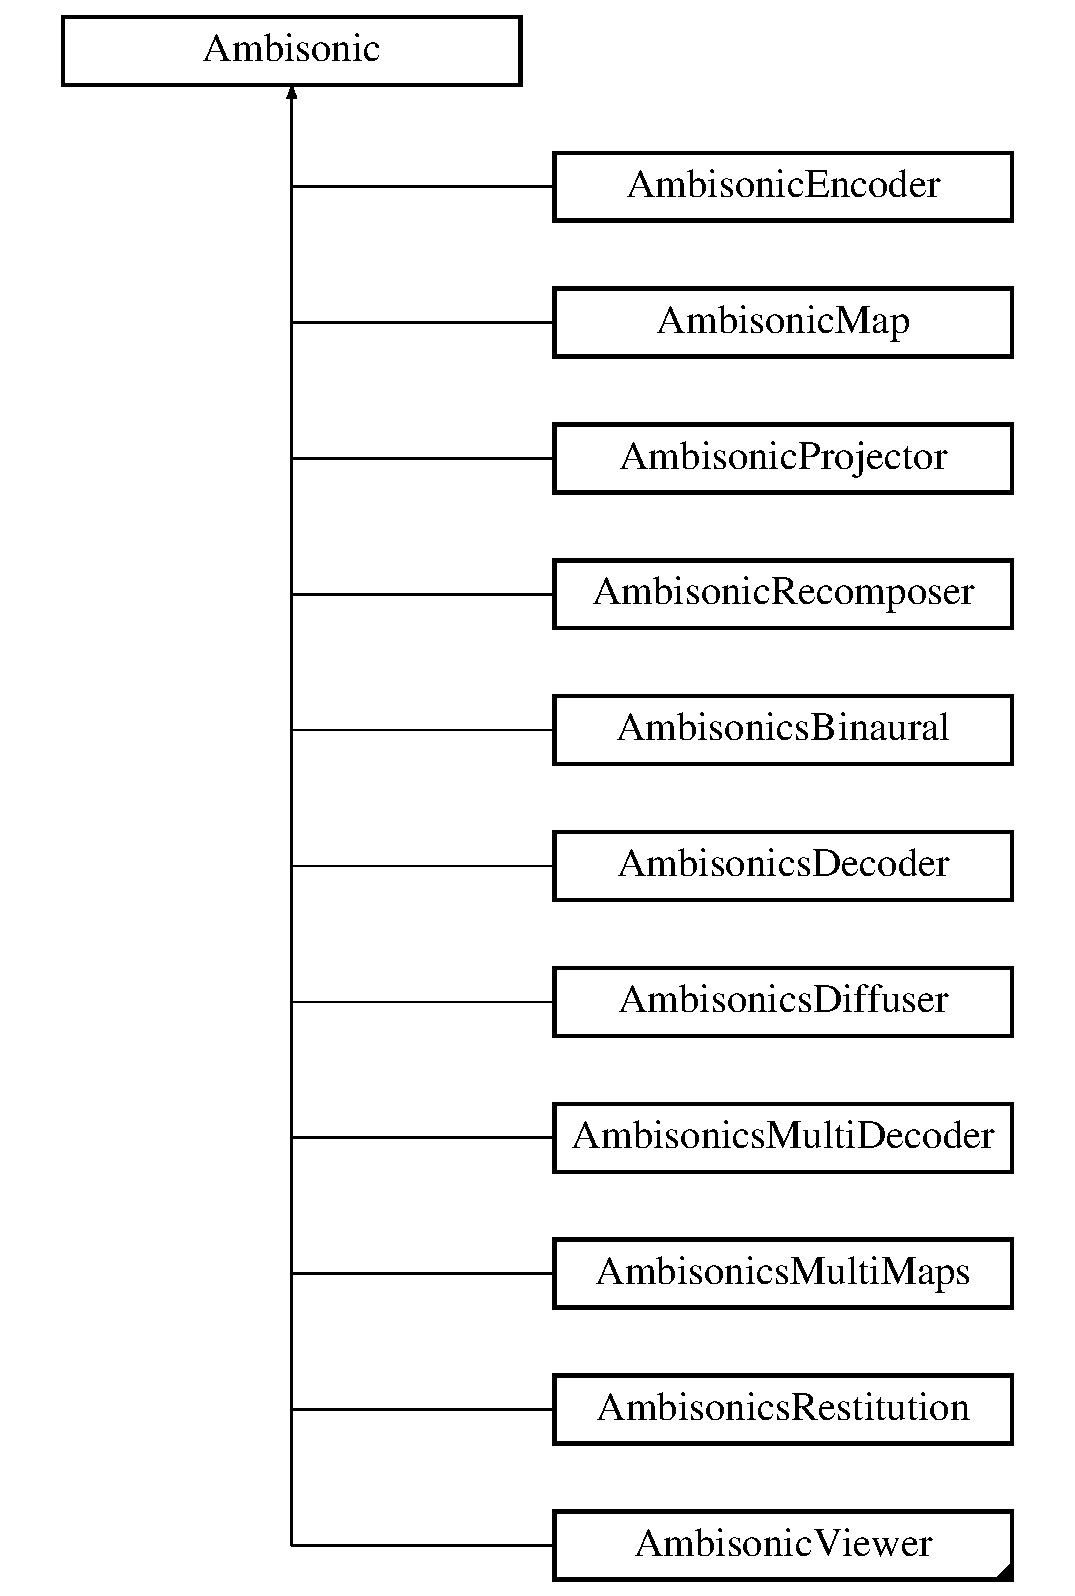
\includegraphics[height=12.000000cm]{class_ambisonic}
\end{center}
\end{figure}
\subsection*{Public Member Functions}
\begin{DoxyCompactItemize}
\item 
\hyperlink{class_ambisonic_ae704cc4472fd1efa22e39f7d501ca7e2}{Ambisonic} (long an\-Order=1, long a\-Vector\-Size=2, long a\-Sampling\-Rate=44100.)
\end{DoxyCompactItemize}


\subsection{Detailed Description}
\hyperlink{interface_hoa_library}{Hoa\-Library} \-: A High Order Ambisonics Library Copyright (c) 2012-\/2013 Julien Colafrancesco, Pierre Guillot, Eliott Paris, C\-I\-C\-M, Universite Paris-\/8. All rights reserved.\-re Guillot, C\-I\-C\-M -\/ Université Paris 8 All rights reserved.

Website \-: \href{http://www.mshparisnord.fr/HoaLibrary/}{\tt http\-://www.\-mshparisnord.\-fr/\-Hoa\-Library/} Contacts \-: \href{mailto:cicm.mshparisnord@gmail.com}{\tt cicm.\-mshparisnord@gmail.\-com}

This file is part of H\-O\-A L\-I\-B\-R\-A\-R\-Y.

H\-O\-A L\-I\-B\-R\-A\-R\-Y is free software\-: you can redistribute it and/or modify it under the terms of the G\-N\-U General Public License as published by the Free Software Foundation, either version 3 of the License, or (at your option) any later version.

This program is distributed in the hope that it will be useful, but W\-I\-T\-H\-O\-U\-T A\-N\-Y W\-A\-R\-R\-A\-N\-T\-Y; without even the implied warranty of M\-E\-R\-C\-H\-A\-N\-T\-A\-B\-I\-L\-I\-T\-Y or F\-I\-T\-N\-E\-S\-S F\-O\-R A P\-A\-R\-T\-I\-C\-U\-L\-A\-R P\-U\-R\-P\-O\-S\-E. See the G\-N\-U General Public License for more details.

You should have received a copy of the G\-N\-U General Public License along with this program. If not, see \href{http://www.gnu.org/licenses/}{\tt http\-://www.\-gnu.\-org/licenses/}. 

Definition at line 32 of file Ambisonic.\-h.



\subsection{Constructor \& Destructor Documentation}
\hypertarget{class_ambisonic_ae704cc4472fd1efa22e39f7d501ca7e2}{\index{Ambisonic@{Ambisonic}!Ambisonic@{Ambisonic}}
\index{Ambisonic@{Ambisonic}!Ambisonic@{Ambisonic}}
\subsubsection[{Ambisonic}]{\setlength{\rightskip}{0pt plus 5cm}Ambisonic\-::\-Ambisonic (
\begin{DoxyParamCaption}
\item[{long}]{an\-Order = {\ttfamily 1}, }
\item[{long}]{a\-Vector\-Size = {\ttfamily 2}, }
\item[{long}]{a\-Sampling\-Rate = {\ttfamily 44100.}}
\end{DoxyParamCaption}
)}}\label{class_ambisonic_ae704cc4472fd1efa22e39f7d501ca7e2}
\hyperlink{interface_hoa_library}{Hoa\-Library} \-: A High Order Ambisonics Library Copyright (c) 2012-\/2013 Julien Colafrancesco, Pierre Guillot, Eliott Paris, C\-I\-C\-M, Universite Paris-\/8. All rights reserved.\-re Guillot, C\-I\-C\-M -\/ Université Paris 8 All rights reserved.

Website \-: \href{http://www.mshparisnord.fr/HoaLibrary/}{\tt http\-://www.\-mshparisnord.\-fr/\-Hoa\-Library/} Contacts \-: \href{mailto:cicm.mshparisnord@gmail.com}{\tt cicm.\-mshparisnord@gmail.\-com}

This file is part of H\-O\-A L\-I\-B\-R\-A\-R\-Y.

H\-O\-A L\-I\-B\-R\-A\-R\-Y is free software\-: you can redistribute it and/or modify it under the terms of the G\-N\-U General Public License as published by the Free Software Foundation, either version 3 of the License, or (at your option) any later version.

This program is distributed in the hope that it will be useful, but W\-I\-T\-H\-O\-U\-T A\-N\-Y W\-A\-R\-R\-A\-N\-T\-Y; without even the implied warranty of M\-E\-R\-C\-H\-A\-N\-T\-A\-B\-I\-L\-I\-T\-Y or F\-I\-T\-N\-E\-S\-S F\-O\-R A P\-A\-R\-T\-I\-C\-U\-L\-A\-R P\-U\-R\-P\-O\-S\-E. See the G\-N\-U General Public License for more details.

You should have received a copy of the G\-N\-U General Public License along with this program. If not, see \href{http://www.gnu.org/licenses/}{\tt http\-://www.\-gnu.\-org/licenses/}. 

Definition at line 29 of file Ambisonic.\-cpp.



The documentation for this class was generated from the following files\-:\begin{DoxyCompactItemize}
\item 
/\-Users/\-Pierre/\-Source\-Tree/\-Hoa\-Library/\-Sources/hoa\-Ambisonics/Ambisonic.\-h\item 
/\-Users/\-Pierre/\-Source\-Tree/\-Hoa\-Library/\-Sources/hoa\-Ambisonics/Ambisonic.\-cpp\end{DoxyCompactItemize}

\hypertarget{class_ambisonic3_d}{\section{Ambisonic3\-D Class Reference}
\label{class_ambisonic3_d}\index{Ambisonic3\-D@{Ambisonic3\-D}}
}


{\ttfamily \#include $<$Ambisonic3\-D.\-h$>$}

Inheritance diagram for Ambisonic3\-D\-:\begin{figure}[H]
\begin{center}
\leavevmode
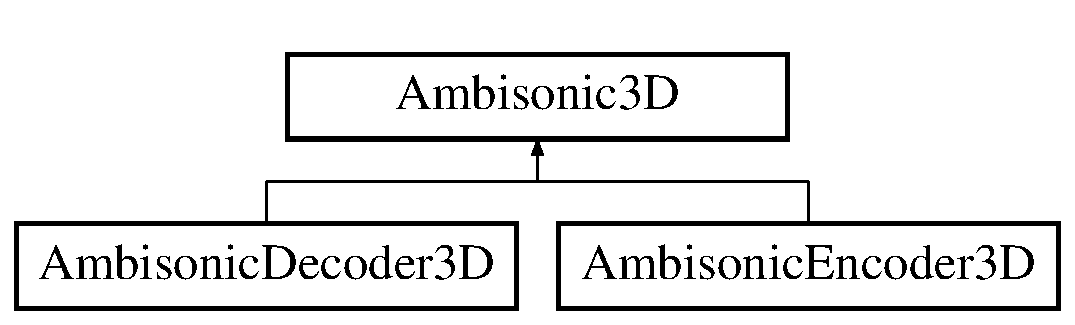
\includegraphics[height=2.000000cm]{class_ambisonic3_d}
\end{center}
\end{figure}
\subsection*{Public Member Functions}
\begin{DoxyCompactItemize}
\item 
\hyperlink{class_ambisonic3_d_aa0948430277ba494551bb712f7a548ea}{Ambisonic3\-D} (long an\-Order=1, long a\-Vector\-Size=2, long a\-Sampling\-Rate=44100.)
\item 
\hypertarget{class_ambisonic3_d_a122f538beab6cecd937494795d9fea68}{long {\bfseries get\-Order} ()}\label{class_ambisonic3_d_a122f538beab6cecd937494795d9fea68}

\item 
\hypertarget{class_ambisonic3_d_a0def8cb523b6f09d704bb78c7104ff6d}{long {\bfseries get\-Number\-Of\-Harmonics} ()}\label{class_ambisonic3_d_a0def8cb523b6f09d704bb78c7104ff6d}

\item 
\hypertarget{class_ambisonic3_d_ad6729e3265d85ebbca09c8dc7b88ae0a}{long {\bfseries get\-Number\-Of\-Inputs} ()}\label{class_ambisonic3_d_ad6729e3265d85ebbca09c8dc7b88ae0a}

\item 
\hypertarget{class_ambisonic3_d_a7c94c05cb033a8f84ae5a92b20896c25}{long {\bfseries get\-Number\-Of\-Outputs} ()}\label{class_ambisonic3_d_a7c94c05cb033a8f84ae5a92b20896c25}

\item 
\hypertarget{class_ambisonic3_d_aa3dfa779bd5934d617fc2cc087421928}{long {\bfseries get\-Vector\-Size} ()}\label{class_ambisonic3_d_aa3dfa779bd5934d617fc2cc087421928}

\item 
\hypertarget{class_ambisonic3_d_afd6071ee65babdcf2ba6f10b5b5fefe0}{long {\bfseries get\-Sampling\-Rate} ()}\label{class_ambisonic3_d_afd6071ee65babdcf2ba6f10b5b5fefe0}

\item 
\hypertarget{class_ambisonic3_d_acff0f5e46b5a7c6de7856956bda1e1a0}{long {\bfseries get\-Harmonic\-Index} (long an\-Index)}\label{class_ambisonic3_d_acff0f5e46b5a7c6de7856956bda1e1a0}

\item 
\hypertarget{class_ambisonic3_d_adcd251db6df904e4cab3e464e19c3a08}{long {\bfseries get\-Harmonic\-Order} (long an\-Index)}\label{class_ambisonic3_d_adcd251db6df904e4cab3e464e19c3a08}

\item 
\hypertarget{class_ambisonic3_d_a77d9738670b3a3224dd622f01eb65689}{std\-::string {\bfseries get\-Harmonics\-Name} (long an\-Index)}\label{class_ambisonic3_d_a77d9738670b3a3224dd622f01eb65689}

\item 
\hypertarget{class_ambisonic3_d_a0da0abc4a0036f369bd84a926ac3734c}{void {\bfseries set\-Vector\-Size} (long a\-Vector\-Size)}\label{class_ambisonic3_d_a0da0abc4a0036f369bd84a926ac3734c}

\item 
\hypertarget{class_ambisonic3_d_a5e7467dbba7233317954b4ed8607174c}{void {\bfseries set\-Sampling\-Rate} (long a\-Sampling\-Rate)}\label{class_ambisonic3_d_a5e7467dbba7233317954b4ed8607174c}

\item 
\hypertarget{class_ambisonic3_d_af5e2e2ed735b2746c5f4a27867bb2459}{void {\bfseries process} (float $\ast$inputs, float $\ast$outputs)}\label{class_ambisonic3_d_af5e2e2ed735b2746c5f4a27867bb2459}

\item 
\hypertarget{class_ambisonic3_d_ae7280e883920d813914e5acdd40139c3}{void {\bfseries process} (double $\ast$inputs, double $\ast$outputs)}\label{class_ambisonic3_d_ae7280e883920d813914e5acdd40139c3}

\item 
\hypertarget{class_ambisonic3_d_a1e0bf1a4a9c40c7b8f576976532a94d3}{void {\bfseries process} (float $\ast$$\ast$inputs, float $\ast$$\ast$outputs)}\label{class_ambisonic3_d_a1e0bf1a4a9c40c7b8f576976532a94d3}

\item 
\hypertarget{class_ambisonic3_d_af678e023c64b3865ef27fe29bcc4a0ca}{void {\bfseries process} (double $\ast$$\ast$inputs, double $\ast$$\ast$outputs)}\label{class_ambisonic3_d_af678e023c64b3865ef27fe29bcc4a0ca}

\end{DoxyCompactItemize}
\subsection*{Protected Attributes}
\begin{DoxyCompactItemize}
\item 
\hypertarget{class_ambisonic3_d_a3ea989a3583e2972139a363564711e2b}{long {\bfseries m\-\_\-order}}\label{class_ambisonic3_d_a3ea989a3583e2972139a363564711e2b}

\item 
\hypertarget{class_ambisonic3_d_aceadaee86c8d9ad770bbe00829e65804}{long {\bfseries m\-\_\-number\-\_\-of\-\_\-harmonics}}\label{class_ambisonic3_d_aceadaee86c8d9ad770bbe00829e65804}

\item 
\hypertarget{class_ambisonic3_d_ace03a703aad689dc3d48e95a9e4f4d06}{long {\bfseries m\-\_\-number\-\_\-of\-\_\-inputs}}\label{class_ambisonic3_d_ace03a703aad689dc3d48e95a9e4f4d06}

\item 
\hypertarget{class_ambisonic3_d_ad650b4479aa106e0914b5aa3634249a0}{long {\bfseries m\-\_\-number\-\_\-of\-\_\-outputs}}\label{class_ambisonic3_d_ad650b4479aa106e0914b5aa3634249a0}

\item 
\hypertarget{class_ambisonic3_d_a07817497c3dad9c59077fb41ec7e7078}{long {\bfseries m\-\_\-vector\-\_\-size}}\label{class_ambisonic3_d_a07817497c3dad9c59077fb41ec7e7078}

\item 
\hypertarget{class_ambisonic3_d_ac9aa7a4977de5f201ab2ee7e4cd9aec7}{long {\bfseries m\-\_\-sampling\-\_\-rate}}\label{class_ambisonic3_d_ac9aa7a4977de5f201ab2ee7e4cd9aec7}

\item 
\hypertarget{class_ambisonic3_d_a6956fcba4f28ef36e487ab84a003ab27}{long $\ast$ {\bfseries m\-\_\-harmonics\-\_\-indices}}\label{class_ambisonic3_d_a6956fcba4f28ef36e487ab84a003ab27}

\item 
\hypertarget{class_ambisonic3_d_a5da35d2fac8aee501c51fd57ec66b565}{long $\ast$ {\bfseries m\-\_\-harmonics\-\_\-orders}}\label{class_ambisonic3_d_a5da35d2fac8aee501c51fd57ec66b565}

\end{DoxyCompactItemize}


\subsection{Detailed Description}
Hoa\-Library \-: A High Order Ambisonics Library Copyright (c) 2012-\/2013 Julien Colafrancesco, Pierre Guillot, Eliott Paris, C\-I\-C\-M, Universite Paris-\/8. All rights reserved.\-re Guillot, C\-I\-C\-M -\/ Université Paris 8 All rights reserved.

Website \-: \href{http://www.mshparisnord.fr/HoaLibrary/}{\tt http\-://www.\-mshparisnord.\-fr/\-Hoa\-Library/} Contacts \-: \href{mailto:cicm.mshparisnord@gmail.com}{\tt cicm.\-mshparisnord@gmail.\-com}

This file is part of H\-O\-A L\-I\-B\-R\-A\-R\-Y.

H\-O\-A L\-I\-B\-R\-A\-R\-Y is free software\-: you can redistribute it and/or modify it under the terms of the G\-N\-U General Public License as published by the Free Software Foundation, either version 3 of the License, or (at your option) any later version.

This program is distributed in the hope that it will be useful, but W\-I\-T\-H\-O\-U\-T A\-N\-Y W\-A\-R\-R\-A\-N\-T\-Y; without even the implied warranty of M\-E\-R\-C\-H\-A\-N\-T\-A\-B\-I\-L\-I\-T\-Y or F\-I\-T\-N\-E\-S\-S F\-O\-R A P\-A\-R\-T\-I\-C\-U\-L\-A\-R P\-U\-R\-P\-O\-S\-E. See the G\-N\-U General Public License for more details.

You should have received a copy of the G\-N\-U General Public License along with this program. If not, see \href{http://www.gnu.org/licenses/}{\tt http\-://www.\-gnu.\-org/licenses/}. 

\subsection{Constructor \& Destructor Documentation}
\hypertarget{class_ambisonic3_d_aa0948430277ba494551bb712f7a548ea}{\index{Ambisonic3\-D@{Ambisonic3\-D}!Ambisonic3\-D@{Ambisonic3\-D}}
\index{Ambisonic3\-D@{Ambisonic3\-D}!Ambisonic3D@{Ambisonic3\-D}}
\subsubsection[{Ambisonic3\-D}]{\setlength{\rightskip}{0pt plus 5cm}Ambisonic3\-D\-::\-Ambisonic3\-D (
\begin{DoxyParamCaption}
\item[{long}]{an\-Order = {\ttfamily 1}, }
\item[{long}]{a\-Vector\-Size = {\ttfamily 2}, }
\item[{long}]{a\-Sampling\-Rate = {\ttfamily 44100.}}
\end{DoxyParamCaption}
)}}\label{class_ambisonic3_d_aa0948430277ba494551bb712f7a548ea}
Hoa\-Library \-: A High Order Ambisonics Library Copyright (c) 2012-\/2013 Julien Colafrancesco, Pierre Guillot, Eliott Paris, C\-I\-C\-M, Universite Paris-\/8. All rights reserved.\-re Guillot, C\-I\-C\-M -\/ Université Paris 8 All rights reserved.

Website \-: \href{http://www.mshparisnord.fr/HoaLibrary/}{\tt http\-://www.\-mshparisnord.\-fr/\-Hoa\-Library/} Contacts \-: \href{mailto:cicm.mshparisnord@gmail.com}{\tt cicm.\-mshparisnord@gmail.\-com}

This file is part of H\-O\-A L\-I\-B\-R\-A\-R\-Y.

H\-O\-A L\-I\-B\-R\-A\-R\-Y is free software\-: you can redistribute it and/or modify it under the terms of the G\-N\-U General Public License as published by the Free Software Foundation, either version 3 of the License, or (at your option) any later version.

This program is distributed in the hope that it will be useful, but W\-I\-T\-H\-O\-U\-T A\-N\-Y W\-A\-R\-R\-A\-N\-T\-Y; without even the implied warranty of M\-E\-R\-C\-H\-A\-N\-T\-A\-B\-I\-L\-I\-T\-Y or F\-I\-T\-N\-E\-S\-S F\-O\-R A P\-A\-R\-T\-I\-C\-U\-L\-A\-R P\-U\-R\-P\-O\-S\-E. See the G\-N\-U General Public License for more details.

You should have received a copy of the G\-N\-U General Public License along with this program. If not, see \href{http://www.gnu.org/licenses/}{\tt http\-://www.\-gnu.\-org/licenses/}. 

The documentation for this class was generated from the following files\-:\begin{DoxyCompactItemize}
\item 
/\-Users/\-Pierre/\-Source\-Tree/\-Hoa\-Library/\-Sources/hoa\-Ambisonics/Ambisonic3\-D.\-h\item 
/\-Users/\-Pierre/\-Source\-Tree/\-Hoa\-Library/\-Sources/hoa\-Ambisonics/Ambisonic3\-D.\-cpp\end{DoxyCompactItemize}

\hypertarget{class_ambisonic_convolver}{\section{Ambisonic\-Convolver Class Reference}
\label{class_ambisonic_convolver}\index{Ambisonic\-Convolver@{Ambisonic\-Convolver}}
}


{\ttfamily \#include $<$Ambisonic\-Convolver.\-h$>$}

Inheritance diagram for Ambisonic\-Convolver\-:\begin{figure}[H]
\begin{center}
\leavevmode
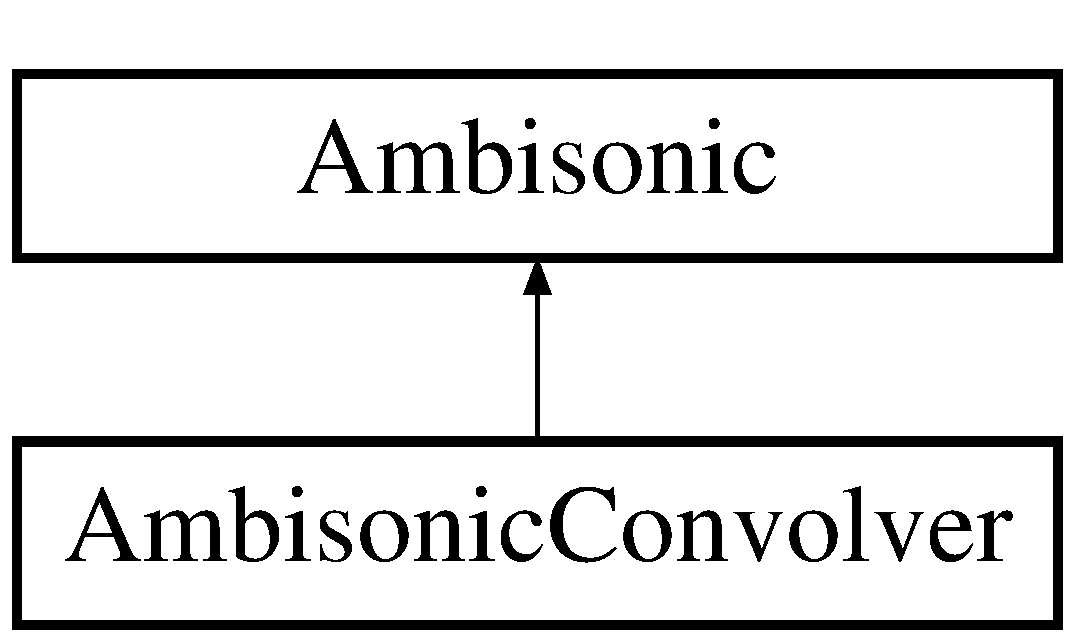
\includegraphics[height=2.000000cm]{class_ambisonic_convolver}
\end{center}
\end{figure}
\subsection*{Public Member Functions}
\begin{DoxyCompactItemize}
\item 
\hyperlink{class_ambisonic_convolver_a738ca279b391cf1adba9e2004ac74c52}{Ambisonic\-Convolver} (long an\-Order=4, long a\-Sampling\-Frequency=44100, long a\-Vector\-Size=0)
\end{DoxyCompactItemize}


\subsection{Detailed Description}
\hyperlink{interface_hoa_library}{Hoa\-Library} \-: A High Order Ambisonics Library Copyright (c) 2012-\/2013 Julien Colafrancesco, Pierre Guillot, Eliott Paris, C\-I\-C\-M, Universite Paris-\/8. All rights reserved.\-re Guillot, C\-I\-C\-M -\/ Université Paris 8 All rights reserved.

Website \-: \href{http://www.mshparisnord.fr/HoaLibrary/}{\tt http\-://www.\-mshparisnord.\-fr/\-Hoa\-Library/} Contacts \-: \href{mailto:cicm.mshparisnord@gmail.com}{\tt cicm.\-mshparisnord@gmail.\-com}

This file is part of H\-O\-A L\-I\-B\-R\-A\-R\-Y.

H\-O\-A L\-I\-B\-R\-A\-R\-Y is free software\-: you can redistribute it and/or modify it under the terms of the G\-N\-U General Public License as published by the Free Software Foundation, either version 3 of the License, or (at your option) any later version.

This program is distributed in the hope that it will be useful, but W\-I\-T\-H\-O\-U\-T A\-N\-Y W\-A\-R\-R\-A\-N\-T\-Y; without even the implied warranty of M\-E\-R\-C\-H\-A\-N\-T\-A\-B\-I\-L\-I\-T\-Y or F\-I\-T\-N\-E\-S\-S F\-O\-R A P\-A\-R\-T\-I\-C\-U\-L\-A\-R P\-U\-R\-P\-O\-S\-E. See the G\-N\-U General Public License for more details.

You should have received a copy of the G\-N\-U General Public License along with this program. If not, see \href{http://www.gnu.org/licenses/}{\tt http\-://www.\-gnu.\-org/licenses/}. 

\subsection{Constructor \& Destructor Documentation}
\hypertarget{class_ambisonic_convolver_a738ca279b391cf1adba9e2004ac74c52}{\index{Ambisonic\-Convolver@{Ambisonic\-Convolver}!Ambisonic\-Convolver@{Ambisonic\-Convolver}}
\index{Ambisonic\-Convolver@{Ambisonic\-Convolver}!AmbisonicConvolver@{Ambisonic\-Convolver}}
\subsubsection[{Ambisonic\-Convolver}]{\setlength{\rightskip}{0pt plus 5cm}Ambisonic\-Convolver\-::\-Ambisonic\-Convolver (
\begin{DoxyParamCaption}
\item[{long}]{an\-Order = {\ttfamily 4}, }
\item[{long}]{a\-Sampling\-Frequency = {\ttfamily 44100}, }
\item[{long}]{a\-Vector\-Size = {\ttfamily 0}}
\end{DoxyParamCaption}
)}}\label{class_ambisonic_convolver_a738ca279b391cf1adba9e2004ac74c52}
\hyperlink{interface_hoa_library}{Hoa\-Library} \-: A High Order Ambisonics Library Copyright (c) 2012-\/2013 Julien Colafrancesco, Pierre Guillot, Eliott Paris, C\-I\-C\-M, Universite Paris-\/8. All rights reserved.

Website \-: \href{http://www.mshparisnord.fr/hoalibrary/}{\tt http\-://www.\-mshparisnord.\-fr/hoalibrary/} Contacts \-: \href{mailto:cicm.mshparisnord@gmail.com}{\tt cicm.\-mshparisnord@gmail.\-com}

Redistribution and use in source and binary forms, with or without modification, are permitted provided that the following conditions are met\-:


\begin{DoxyItemize}
\item Redistributions may not be sold, nor may they be used in a commercial product or activity.
\item Redistributions of source code must retain the above copyright notice, this list of conditions and the following disclaimer.
\item Redistributions in binary form must reproduce the above copyright notice, this list of conditions and the following disclaimer in the documentation and/or other materials provided with the distribution.
\item Neither the name of the C\-I\-C\-M nor the names of its contributors may be used to endorse or promote products derived from this software without specific prior written permission.
\end{DoxyItemize}

T\-H\-I\-S S\-O\-F\-T\-W\-A\-R\-E I\-S P\-R\-O\-V\-I\-D\-E\-D B\-Y T\-H\-E C\-O\-P\-Y\-R\-I\-G\-H\-T H\-O\-L\-D\-E\-R\-S A\-N\-D C\-O\-N\-T\-R\-I\-B\-U\-T\-O\-R\-S \char`\"{}\-A\-S I\-S\char`\"{} A\-N\-D A\-N\-Y E\-X\-P\-R\-E\-S\-S O\-R I\-M\-P\-L\-I\-E\-D W\-A\-R\-R\-A\-N\-T\-I\-E\-S, I\-N\-C\-L\-U\-D\-I\-N\-G, B\-U\-T N\-O\-T L\-I\-M\-I\-T\-E\-D T\-O, T\-H\-E I\-M\-P\-L\-I\-E\-D W\-A\-R\-R\-A\-N\-T\-I\-E\-S O\-F M\-E\-R\-C\-H\-A\-N\-T\-A\-B\-I\-L\-I\-T\-Y A\-N\-D F\-I\-T\-N\-E\-S\-S F\-O\-R A P\-A\-R\-T\-I\-C\-U\-L\-A\-R P\-U\-R\-P\-O\-S\-E A\-R\-E D\-I\-S\-C\-L\-A\-I\-M\-E\-D. I\-N N\-O E\-V\-E\-N\-T S\-H\-A\-L\-L T\-H\-E C\-O\-P\-Y\-R\-I\-G\-H\-T H\-O\-L\-D\-E\-R O\-R C\-O\-N\-T\-R\-I\-B\-U\-T\-O\-R\-S B\-E L\-I\-A\-B\-L\-E F\-O\-R A\-N\-Y D\-I\-R\-E\-C\-T, I\-N\-D\-I\-R\-E\-C\-T, I\-N\-C\-I\-D\-E\-N\-T\-A\-L, S\-P\-E\-C\-I\-A\-L, E\-X\-E\-M\-P\-L\-A\-R\-Y, O\-R C\-O\-N\-S\-E\-Q\-U\-E\-N\-T\-I\-A\-L D\-A\-M\-A\-G\-E\-S (I\-N\-C\-L\-U\-D\-I\-N\-G, B\-U\-T N\-O\-T L\-I\-M\-I\-T\-E\-D T\-O, P\-R\-O\-C\-U\-R\-E\-M\-E\-N\-T O\-F S\-U\-B\-S\-T\-I\-T\-U\-T\-E G\-O\-O\-D\-S O\-R S\-E\-R\-V\-I\-C\-E\-S; L\-O\-S\-S O\-F U\-S\-E, D\-A\-T\-A, O\-R P\-R\-O\-F\-I\-T\-S; O\-R B\-U\-S\-I\-N\-E\-S\-S I\-N\-T\-E\-R\-R\-U\-P\-T\-I\-O\-N) H\-O\-W\-E\-V\-E\-R C\-A\-U\-S\-E\-D A\-N\-D O\-N A\-N\-Y T\-H\-E\-O\-R\-Y O\-F L\-I\-A\-B\-I\-L\-I\-T\-Y, W\-H\-E\-T\-H\-E\-R I\-N C\-O\-N\-T\-R\-A\-C\-T, S\-T\-R\-I\-C\-T L\-I\-A\-B\-I\-L\-I\-T\-Y, O\-R T\-O\-R\-T (I\-N\-C\-L\-U\-D\-I\-N\-G N\-E\-G\-L\-I\-G\-E\-N\-C\-E O\-R O\-T\-H\-E\-R\-W\-I\-S\-E) A\-R\-I\-S\-I\-N\-G I\-N A\-N\-Y W\-A\-Y O\-U\-T O\-F T\-H\-E U\-S\-E O\-F T\-H\-I\-S S\-O\-F\-T\-W\-A\-R\-E, E\-V\-E\-N I\-F A\-D\-V\-I\-S\-E\-D O\-F T\-H\-E P\-O\-S\-S\-I\-B\-I\-L\-I\-T\-Y O\-F S\-U\-C\-H D\-A\-M\-A\-G\-E. 

The documentation for this class was generated from the following files\-:\begin{DoxyCompactItemize}
\item 
/\-Users/\-Pierre/\-Source\-Tree/\-Hoa\-Library/\-Sources/hoa\-Convolve/Ambisonic\-Convolver.\-h\item 
/\-Users/\-Pierre/\-Source\-Tree/\-Hoa\-Library/\-Sources/hoa\-Convolve/Ambisonic\-Convolver.\-cpp\end{DoxyCompactItemize}

\hypertarget{class_ambisonic_decoder3_d}{\section{Ambisonic\-Decoder3\-D Class Reference}
\label{class_ambisonic_decoder3_d}\index{Ambisonic\-Decoder3\-D@{Ambisonic\-Decoder3\-D}}
}
Inheritance diagram for Ambisonic\-Decoder3\-D\-:\begin{figure}[H]
\begin{center}
\leavevmode
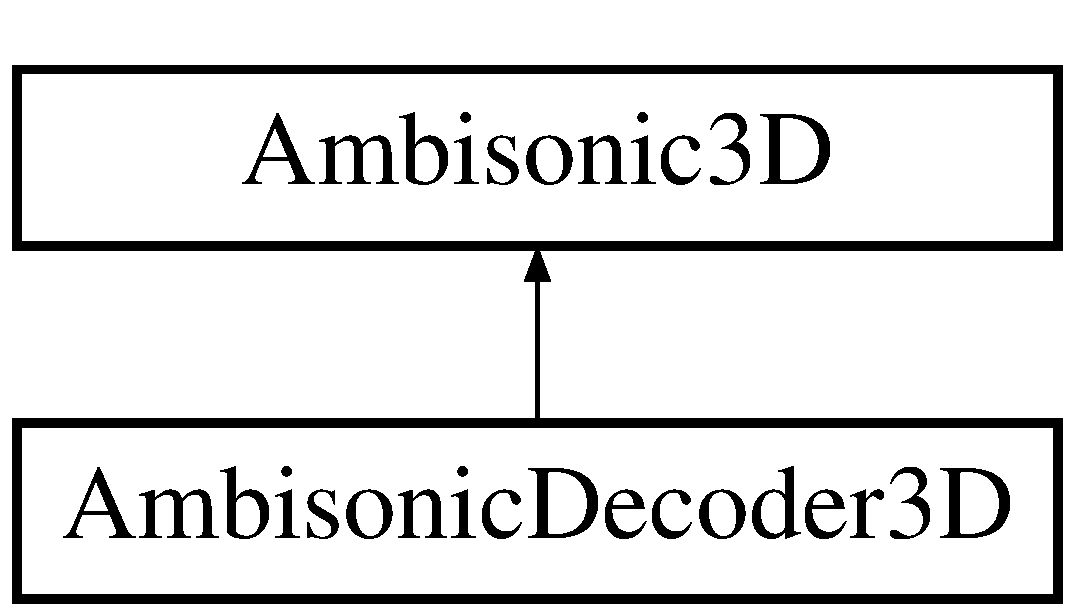
\includegraphics[height=2.000000cm]{class_ambisonic_decoder3_d}
\end{center}
\end{figure}
\subsection*{Public Member Functions}
\begin{DoxyCompactItemize}
\item 
\hyperlink{class_ambisonic_decoder3_d_a500aa4620487dc857bd1c2c89acfe874}{Ambisonic\-Decoder3\-D} (long an\-Order=1, long a\-Number\-Of\-Loudspeakers=8, bool a\-Shape=Hoa\-\_\-\-Full\-\_\-\-Sphere, long a\-Vector\-Size=2, long a\-Samling\-Rate=44100)
\item 
\hypertarget{class_ambisonic_decoder3_d_a910db37deb4ad6fd574a43d692888842}{void {\bfseries set\-Number\-Of\-Loudspeakers} (long a\-Number\-Of\-Loudspeakers, bool a\-Shape=Hoa\-\_\-\-Full\-\_\-\-Sphere)}\label{class_ambisonic_decoder3_d_a910db37deb4ad6fd574a43d692888842}

\item 
\hypertarget{class_ambisonic_decoder3_d_a646c9ad31367db67b001964be4692145}{void {\bfseries set\-Loudspeaker\-Position} (long an\-Index, double an\-Azimuth, double an\-Elevation)}\label{class_ambisonic_decoder3_d_a646c9ad31367db67b001964be4692145}

\item 
\hypertarget{class_ambisonic_decoder3_d_a5942ef0cad58db519d4bc28d7422b3fc}{double {\bfseries get\-Loudspeaker\-Azimuth} (long an\-Index)}\label{class_ambisonic_decoder3_d_a5942ef0cad58db519d4bc28d7422b3fc}

\item 
\hypertarget{class_ambisonic_decoder3_d_a90aff96227bfdbde571bb26998af9750}{double {\bfseries get\-Loudspeaker\-Elevation} (long an\-Index)}\label{class_ambisonic_decoder3_d_a90aff96227bfdbde571bb26998af9750}

\item 
\hypertarget{class_ambisonic_decoder3_d_adb378983f0ac5c5dbb27f69f02fd2993}{void {\bfseries process} (const float $\ast$an\-Input, float $\ast$an\-Output)}\label{class_ambisonic_decoder3_d_adb378983f0ac5c5dbb27f69f02fd2993}

\item 
\hypertarget{class_ambisonic_decoder3_d_aacbe0f5139bc59edd8b12693d84388b6}{void {\bfseries process} (const double $\ast$an\-Input, double $\ast$an\-Output)}\label{class_ambisonic_decoder3_d_aacbe0f5139bc59edd8b12693d84388b6}

\end{DoxyCompactItemize}
\subsection*{Additional Inherited Members}


\subsection{Constructor \& Destructor Documentation}
\hypertarget{class_ambisonic_decoder3_d_a500aa4620487dc857bd1c2c89acfe874}{\index{Ambisonic\-Decoder3\-D@{Ambisonic\-Decoder3\-D}!Ambisonic\-Decoder3\-D@{Ambisonic\-Decoder3\-D}}
\index{Ambisonic\-Decoder3\-D@{Ambisonic\-Decoder3\-D}!AmbisonicDecoder3D@{Ambisonic\-Decoder3\-D}}
\subsubsection[{Ambisonic\-Decoder3\-D}]{\setlength{\rightskip}{0pt plus 5cm}Ambisonic\-Decoder3\-D\-::\-Ambisonic\-Decoder3\-D (
\begin{DoxyParamCaption}
\item[{long}]{an\-Order = {\ttfamily 1}, }
\item[{long}]{a\-Number\-Of\-Loudspeakers = {\ttfamily 8}, }
\item[{bool}]{a\-Shape = {\ttfamily Hoa\-\_\-Full\-\_\-Sphere}, }
\item[{long}]{a\-Vector\-Size = {\ttfamily 2}, }
\item[{long}]{a\-Samling\-Rate = {\ttfamily 44100}}
\end{DoxyParamCaption}
)}}\label{class_ambisonic_decoder3_d_a500aa4620487dc857bd1c2c89acfe874}
\hyperlink{interface_hoa_library}{Hoa\-Library} \-: A High Order Ambisonics Library Copyright (c) 2012-\/2013 Julien Colafrancesco, Pierre Guillot, Eliott Paris, C\-I\-C\-M, Universite Paris-\/8. All rights reserved.

Website \-: \href{http://www.mshparisnord.fr/hoalibrary/}{\tt http\-://www.\-mshparisnord.\-fr/hoalibrary/} Contacts \-: \href{mailto:cicm.mshparisnord@gmail.com}{\tt cicm.\-mshparisnord@gmail.\-com}

Redistribution and use in source and binary forms, with or without modification, are permitted provided that the following conditions are met\-:


\begin{DoxyItemize}
\item Redistributions may not be sold, nor may they be used in a commercial product or activity.
\item Redistributions of source code must retain the above copyright notice, this list of conditions and the following disclaimer.
\item Redistributions in binary form must reproduce the above copyright notice, this list of conditions and the following disclaimer in the documentation and/or other materials provided with the distribution.
\item Neither the name of the C\-I\-C\-M nor the names of its contributors may be used to endorse or promote products derived from this software without specific prior written permission.
\end{DoxyItemize}

T\-H\-I\-S S\-O\-F\-T\-W\-A\-R\-E I\-S P\-R\-O\-V\-I\-D\-E\-D B\-Y T\-H\-E C\-O\-P\-Y\-R\-I\-G\-H\-T H\-O\-L\-D\-E\-R\-S A\-N\-D C\-O\-N\-T\-R\-I\-B\-U\-T\-O\-R\-S \char`\"{}\-A\-S I\-S\char`\"{} A\-N\-D A\-N\-Y E\-X\-P\-R\-E\-S\-S O\-R I\-M\-P\-L\-I\-E\-D W\-A\-R\-R\-A\-N\-T\-I\-E\-S, I\-N\-C\-L\-U\-D\-I\-N\-G, B\-U\-T N\-O\-T L\-I\-M\-I\-T\-E\-D T\-O, T\-H\-E I\-M\-P\-L\-I\-E\-D W\-A\-R\-R\-A\-N\-T\-I\-E\-S O\-F M\-E\-R\-C\-H\-A\-N\-T\-A\-B\-I\-L\-I\-T\-Y A\-N\-D F\-I\-T\-N\-E\-S\-S F\-O\-R A P\-A\-R\-T\-I\-C\-U\-L\-A\-R P\-U\-R\-P\-O\-S\-E A\-R\-E D\-I\-S\-C\-L\-A\-I\-M\-E\-D. I\-N N\-O E\-V\-E\-N\-T S\-H\-A\-L\-L T\-H\-E C\-O\-P\-Y\-R\-I\-G\-H\-T H\-O\-L\-D\-E\-R O\-R C\-O\-N\-T\-R\-I\-B\-U\-T\-O\-R\-S B\-E L\-I\-A\-B\-L\-E F\-O\-R A\-N\-Y D\-I\-R\-E\-C\-T, I\-N\-D\-I\-R\-E\-C\-T, I\-N\-C\-I\-D\-E\-N\-T\-A\-L, S\-P\-E\-C\-I\-A\-L, E\-X\-E\-M\-P\-L\-A\-R\-Y, O\-R C\-O\-N\-S\-E\-Q\-U\-E\-N\-T\-I\-A\-L D\-A\-M\-A\-G\-E\-S (I\-N\-C\-L\-U\-D\-I\-N\-G, B\-U\-T N\-O\-T L\-I\-M\-I\-T\-E\-D T\-O, P\-R\-O\-C\-U\-R\-E\-M\-E\-N\-T O\-F S\-U\-B\-S\-T\-I\-T\-U\-T\-E G\-O\-O\-D\-S O\-R S\-E\-R\-V\-I\-C\-E\-S; L\-O\-S\-S O\-F U\-S\-E, D\-A\-T\-A, O\-R P\-R\-O\-F\-I\-T\-S; O\-R B\-U\-S\-I\-N\-E\-S\-S I\-N\-T\-E\-R\-R\-U\-P\-T\-I\-O\-N) H\-O\-W\-E\-V\-E\-R C\-A\-U\-S\-E\-D A\-N\-D O\-N A\-N\-Y T\-H\-E\-O\-R\-Y O\-F L\-I\-A\-B\-I\-L\-I\-T\-Y, W\-H\-E\-T\-H\-E\-R I\-N C\-O\-N\-T\-R\-A\-C\-T, S\-T\-R\-I\-C\-T L\-I\-A\-B\-I\-L\-I\-T\-Y, O\-R T\-O\-R\-T (I\-N\-C\-L\-U\-D\-I\-N\-G N\-E\-G\-L\-I\-G\-E\-N\-C\-E O\-R O\-T\-H\-E\-R\-W\-I\-S\-E) A\-R\-I\-S\-I\-N\-G I\-N A\-N\-Y W\-A\-Y O\-U\-T O\-F T\-H\-E U\-S\-E O\-F T\-H\-I\-S S\-O\-F\-T\-W\-A\-R\-E, E\-V\-E\-N I\-F A\-D\-V\-I\-S\-E\-D O\-F T\-H\-E P\-O\-S\-S\-I\-B\-I\-L\-I\-T\-Y O\-F S\-U\-C\-H D\-A\-M\-A\-G\-E. 

The documentation for this class was generated from the following files\-:\begin{DoxyCompactItemize}
\item 
/\-Users/\-Pierre/\-Source\-Tree/\-Hoa\-Library/\-Sources/hoa\-Decoder/Ambisonic\-Decoder3\-D.\-h\item 
/\-Users/\-Pierre/\-Source\-Tree/\-Hoa\-Library/\-Sources/hoa\-Decoder/Ambisonic\-Decoder3\-D.\-cpp\end{DoxyCompactItemize}

\hypertarget{class_ambisonic_encoder}{\section{Ambisonic\-Encoder Class Reference}
\label{class_ambisonic_encoder}\index{Ambisonic\-Encoder@{Ambisonic\-Encoder}}
}


An ambisonic encoder.  




{\ttfamily \#include $<$Ambisonic\-Encoder.\-h$>$}

Inheritance diagram for Ambisonic\-Encoder\-:\begin{figure}[H]
\begin{center}
\leavevmode
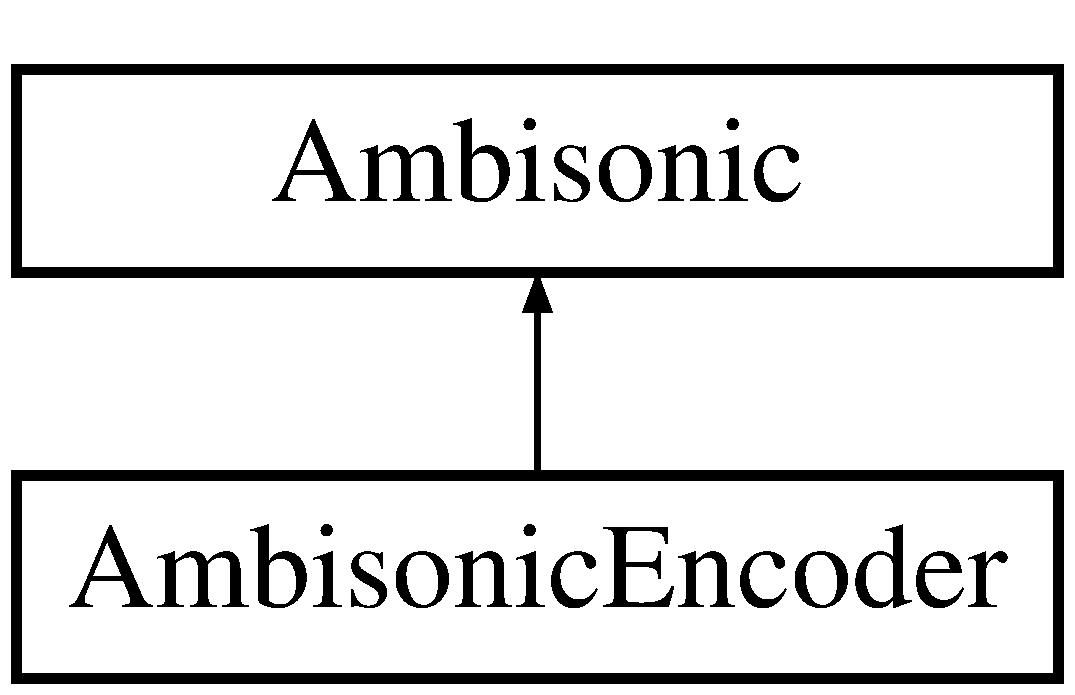
\includegraphics[height=2.000000cm]{class_ambisonic_encoder}
\end{center}
\end{figure}
\subsection*{Public Member Functions}
\begin{DoxyCompactItemize}
\item 
\hyperlink{class_ambisonic_encoder_acf62830cd4a81423886be0f298fc0705}{Ambisonic\-Encoder} (long an\-Order=1, long a\-Vector\-Size=0)
\begin{DoxyCompactList}\small\item\em The encoder constructor. \end{DoxyCompactList}\item 
\hypertarget{class_ambisonic_encoder_a99cb2fbfd9c75c9fac713aff3bc61f54}{\hyperlink{class_ambisonic_encoder_a99cb2fbfd9c75c9fac713aff3bc61f54}{$\sim$\-Ambisonic\-Encoder} ()}\label{class_ambisonic_encoder_a99cb2fbfd9c75c9fac713aff3bc61f54}

\begin{DoxyCompactList}\small\item\em The encoder destructor. \end{DoxyCompactList}\item 
void \hyperlink{class_ambisonic_encoder_a7219775383a3bead41ec7f1a609a76fe}{set\-Vector\-Size} (long a\-Vector\-Size)
\begin{DoxyCompactList}\small\item\em The vector size setter. \end{DoxyCompactList}\item 
void \hyperlink{class_ambisonic_encoder_a1939dfd1305bd3b9387c7bf91b230e35}{set\-Angle} (double an\-Angle)
\begin{DoxyCompactList}\small\item\em The angle setter. \end{DoxyCompactList}\item 
void \hyperlink{class_ambisonic_encoder_a62b6e35d4e281d2f405a03c20a64ca90}{process} (const double input, double $\ast$outputs)
\begin{DoxyCompactList}\small\item\em The sample by sample perform method -\/ double precision -\/ not in place. \end{DoxyCompactList}\item 
void \hyperlink{class_ambisonic_encoder_a06fcd9168c9576c6c73f9bf81019af54}{process} (const float input, float $\ast$outputs)
\begin{DoxyCompactList}\small\item\em The sample by sample perform method -\/ single precision -\/ not in place. \end{DoxyCompactList}\item 
void \hyperlink{class_ambisonic_encoder_a6c8dcafeb8647c15d18fafa71cf52ad7}{process} (const double input, double $\ast$outputs, const double angle)
\begin{DoxyCompactList}\small\item\em The sample by sample perform method with angle -\/ double precision -\/ not in place. \end{DoxyCompactList}\item 
void \hyperlink{class_ambisonic_encoder_a70e57ebbe763cbca011164bc83884dcd}{process} (const float input, float $\ast$outputs, const float angle)
\begin{DoxyCompactList}\small\item\em The sample by sample perform method with angle -\/ single precision -\/ not in place. \end{DoxyCompactList}\item 
void \hyperlink{class_ambisonic_encoder_a7e5cfedb354f5ad134aa19a76a1f61e6}{process} (double $\ast$io\-Vector)
\begin{DoxyCompactList}\small\item\em The sample by sample perform method -\/ double precision -\/ in place. \end{DoxyCompactList}\item 
void \hyperlink{class_ambisonic_encoder_ac8db5ffd1663fd64d8f8e9c701854088}{process} (float $\ast$io\-Vector)
\begin{DoxyCompactList}\small\item\em The sample by sample perform method -\/ single precision -\/ in place. \end{DoxyCompactList}\item 
void \hyperlink{class_ambisonic_encoder_ac68ce0e05589431e54efd91384787e79}{process} (double $\ast$io\-Vector, const double angle)
\begin{DoxyCompactList}\small\item\em The sample by sample perform method with angle -\/ double precision -\/ in place. \end{DoxyCompactList}\item 
void \hyperlink{class_ambisonic_encoder_ab77e6db3e31015c42a066f0f3a6e9a53}{process} (float $\ast$io\-Vector, const float angle)
\begin{DoxyCompactList}\small\item\em The sample by sample perform method with angle -\/ double precision -\/ in place. \end{DoxyCompactList}\end{DoxyCompactItemize}


\subsection{Detailed Description}
An ambisonic encoder. 

\hyperlink{interface_hoa_library}{Hoa\-Library} \-: A High Order Ambisonics Library Copyright (c) 2012-\/2013 Julien Colafrancesco, Pierre Guillot, Eliott Paris, C\-I\-C\-M, Universite Paris-\/8. All rights reserved.\-re Guillot, C\-I\-C\-M -\/ Université Paris 8 All rights reserved.

Website \-: \href{http://www.mshparisnord.fr/HoaLibrary/}{\tt http\-://www.\-mshparisnord.\-fr/\-Hoa\-Library/} Contacts \-: \href{mailto:cicm.mshparisnord@gmail.com}{\tt cicm.\-mshparisnord@gmail.\-com}

This file is part of H\-O\-A L\-I\-B\-R\-A\-R\-Y.

H\-O\-A L\-I\-B\-R\-A\-R\-Y is free software\-: you can redistribute it and/or modify it under the terms of the G\-N\-U General Public License as published by the Free Software Foundation, either version 3 of the License, or (at your option) any later version.

This program is distributed in the hope that it will be useful, but W\-I\-T\-H\-O\-U\-T A\-N\-Y W\-A\-R\-R\-A\-N\-T\-Y; without even the implied warranty of M\-E\-R\-C\-H\-A\-N\-T\-A\-B\-I\-L\-I\-T\-Y or F\-I\-T\-N\-E\-S\-S F\-O\-R A P\-A\-R\-T\-I\-C\-U\-L\-A\-R P\-U\-R\-P\-O\-S\-E. See the G\-N\-U General Public License for more details.

You should have received a copy of the G\-N\-U General Public License along with this program. If not, see \href{http://www.gnu.org/licenses/}{\tt http\-://www.\-gnu.\-org/licenses/}.

The class encodes a signal in the circular harmonics domain depending of an angle (azimuth) and a given order. 

Definition at line 36 of file Ambisonic\-Encoder.\-h.



\subsection{Constructor \& Destructor Documentation}
\hypertarget{class_ambisonic_encoder_acf62830cd4a81423886be0f298fc0705}{\index{Ambisonic\-Encoder@{Ambisonic\-Encoder}!Ambisonic\-Encoder@{Ambisonic\-Encoder}}
\index{Ambisonic\-Encoder@{Ambisonic\-Encoder}!AmbisonicEncoder@{Ambisonic\-Encoder}}
\subsubsection[{Ambisonic\-Encoder}]{\setlength{\rightskip}{0pt plus 5cm}Ambisonic\-Encoder\-::\-Ambisonic\-Encoder (
\begin{DoxyParamCaption}
\item[{long}]{an\-Order = {\ttfamily 1}, }
\item[{long}]{a\-Vector\-Size = {\ttfamily 0}}
\end{DoxyParamCaption}
)}}\label{class_ambisonic_encoder_acf62830cd4a81423886be0f298fc0705}


The encoder constructor. 


\begin{DoxyParams}{Parameters}
{\em an\-Order} & The ambisonic decomposition order. \\
\hline
{\em a\-Vector\-Size} & The size of the samples block.\\
\hline
\end{DoxyParams}
\hyperlink{interface_hoa_library}{Hoa\-Library} \-: A High Order Ambisonics Library Copyright (c) 2012-\/2013 Julien Colafrancesco, Pierre Guillot, Eliott Paris, C\-I\-C\-M, Universite Paris-\/8. All rights reserved.\-re Guillot, C\-I\-C\-M -\/ Université Paris 8 All rights reserved.

Website \-: \href{http://www.mshparisnord.fr/HoaLibrary/}{\tt http\-://www.\-mshparisnord.\-fr/\-Hoa\-Library/} Contacts \-: \href{mailto:cicm.mshparisnord@gmail.com}{\tt cicm.\-mshparisnord@gmail.\-com}

This file is part of H\-O\-A L\-I\-B\-R\-A\-R\-Y.

H\-O\-A L\-I\-B\-R\-A\-R\-Y is free software\-: you can redistribute it and/or modify it under the terms of the G\-N\-U General Public License as published by the Free Software Foundation, either version 3 of the License, or (at your option) any later version.

This program is distributed in the hope that it will be useful, but W\-I\-T\-H\-O\-U\-T A\-N\-Y W\-A\-R\-R\-A\-N\-T\-Y; without even the implied warranty of M\-E\-R\-C\-H\-A\-N\-T\-A\-B\-I\-L\-I\-T\-Y or F\-I\-T\-N\-E\-S\-S F\-O\-R A P\-A\-R\-T\-I\-C\-U\-L\-A\-R P\-U\-R\-P\-O\-S\-E. See the G\-N\-U General Public License for more details.

You should have received a copy of the G\-N\-U General Public License along with this program. If not, see \href{http://www.gnu.org/licenses/}{\tt http\-://www.\-gnu.\-org/licenses/}. 

Definition at line 29 of file Ambisonic\-Encoder.\-cpp.



\subsection{Member Function Documentation}
\hypertarget{class_ambisonic_encoder_a62b6e35d4e281d2f405a03c20a64ca90}{\index{Ambisonic\-Encoder@{Ambisonic\-Encoder}!process@{process}}
\index{process@{process}!AmbisonicEncoder@{Ambisonic\-Encoder}}
\subsubsection[{process}]{\setlength{\rightskip}{0pt plus 5cm}void Ambisonic\-Encoder\-::process (
\begin{DoxyParamCaption}
\item[{const double}]{input, }
\item[{double $\ast$}]{outputs}
\end{DoxyParamCaption}
)\hspace{0.3cm}{\ttfamily [inline]}}}\label{class_ambisonic_encoder_a62b6e35d4e281d2f405a03c20a64ca90}


The sample by sample perform method -\/ double precision -\/ not in place. 


\begin{DoxyParams}{Parameters}
{\em input} & The input sample. \\
\hline
{\em outputs} & The harmonics output array. \\
\hline
\end{DoxyParams}


Definition at line 81 of file Ambisonic\-Encoder.\-h.

\hypertarget{class_ambisonic_encoder_a06fcd9168c9576c6c73f9bf81019af54}{\index{Ambisonic\-Encoder@{Ambisonic\-Encoder}!process@{process}}
\index{process@{process}!AmbisonicEncoder@{Ambisonic\-Encoder}}
\subsubsection[{process}]{\setlength{\rightskip}{0pt plus 5cm}void Ambisonic\-Encoder\-::process (
\begin{DoxyParamCaption}
\item[{const float}]{input, }
\item[{float $\ast$}]{outputs}
\end{DoxyParamCaption}
)\hspace{0.3cm}{\ttfamily [inline]}}}\label{class_ambisonic_encoder_a06fcd9168c9576c6c73f9bf81019af54}


The sample by sample perform method -\/ single precision -\/ not in place. 


\begin{DoxyParams}{Parameters}
{\em input} & The input sample. \\
\hline
{\em outputs} & The harmonics output array. \\
\hline
\end{DoxyParams}


Definition at line 91 of file Ambisonic\-Encoder.\-h.

\hypertarget{class_ambisonic_encoder_a6c8dcafeb8647c15d18fafa71cf52ad7}{\index{Ambisonic\-Encoder@{Ambisonic\-Encoder}!process@{process}}
\index{process@{process}!AmbisonicEncoder@{Ambisonic\-Encoder}}
\subsubsection[{process}]{\setlength{\rightskip}{0pt plus 5cm}void Ambisonic\-Encoder\-::process (
\begin{DoxyParamCaption}
\item[{const double}]{input, }
\item[{double $\ast$}]{outputs, }
\item[{const double}]{angle}
\end{DoxyParamCaption}
)\hspace{0.3cm}{\ttfamily [inline]}}}\label{class_ambisonic_encoder_a6c8dcafeb8647c15d18fafa71cf52ad7}


The sample by sample perform method with angle -\/ double precision -\/ not in place. 


\begin{DoxyParams}{Parameters}
{\em input} & The input sample. \\
\hline
{\em outputs} & The harmonics output array. \\
\hline
{\em angle} & The angle of encoding in radian. \\
\hline
\end{DoxyParams}


Definition at line 102 of file Ambisonic\-Encoder.\-h.

\hypertarget{class_ambisonic_encoder_a70e57ebbe763cbca011164bc83884dcd}{\index{Ambisonic\-Encoder@{Ambisonic\-Encoder}!process@{process}}
\index{process@{process}!AmbisonicEncoder@{Ambisonic\-Encoder}}
\subsubsection[{process}]{\setlength{\rightskip}{0pt plus 5cm}void Ambisonic\-Encoder\-::process (
\begin{DoxyParamCaption}
\item[{const float}]{input, }
\item[{float $\ast$}]{outputs, }
\item[{const float}]{angle}
\end{DoxyParamCaption}
)\hspace{0.3cm}{\ttfamily [inline]}}}\label{class_ambisonic_encoder_a70e57ebbe763cbca011164bc83884dcd}


The sample by sample perform method with angle -\/ single precision -\/ not in place. 


\begin{DoxyParams}{Parameters}
{\em input} & The input sample. \\
\hline
{\em outputs} & The harmonics output array. \\
\hline
{\em angle} & The angle of encoding in radian. \\
\hline
\end{DoxyParams}


Definition at line 118 of file Ambisonic\-Encoder.\-h.

\hypertarget{class_ambisonic_encoder_a7e5cfedb354f5ad134aa19a76a1f61e6}{\index{Ambisonic\-Encoder@{Ambisonic\-Encoder}!process@{process}}
\index{process@{process}!AmbisonicEncoder@{Ambisonic\-Encoder}}
\subsubsection[{process}]{\setlength{\rightskip}{0pt plus 5cm}void Ambisonic\-Encoder\-::process (
\begin{DoxyParamCaption}
\item[{double $\ast$}]{io\-Vector}
\end{DoxyParamCaption}
)\hspace{0.3cm}{\ttfamily [inline]}}}\label{class_ambisonic_encoder_a7e5cfedb354f5ad134aa19a76a1f61e6}


The sample by sample perform method -\/ double precision -\/ in place. 


\begin{DoxyParams}{Parameters}
{\em io\-Vector} & The input sample and harmonics output array. \\
\hline
\end{DoxyParams}


Definition at line 133 of file Ambisonic\-Encoder.\-h.

\hypertarget{class_ambisonic_encoder_ac8db5ffd1663fd64d8f8e9c701854088}{\index{Ambisonic\-Encoder@{Ambisonic\-Encoder}!process@{process}}
\index{process@{process}!AmbisonicEncoder@{Ambisonic\-Encoder}}
\subsubsection[{process}]{\setlength{\rightskip}{0pt plus 5cm}void Ambisonic\-Encoder\-::process (
\begin{DoxyParamCaption}
\item[{float $\ast$}]{io\-Vector}
\end{DoxyParamCaption}
)\hspace{0.3cm}{\ttfamily [inline]}}}\label{class_ambisonic_encoder_ac8db5ffd1663fd64d8f8e9c701854088}


The sample by sample perform method -\/ single precision -\/ in place. 


\begin{DoxyParams}{Parameters}
{\em io\-Vector} & The input sample and harmonics output array. \\
\hline
\end{DoxyParams}


Definition at line 143 of file Ambisonic\-Encoder.\-h.

\hypertarget{class_ambisonic_encoder_ac68ce0e05589431e54efd91384787e79}{\index{Ambisonic\-Encoder@{Ambisonic\-Encoder}!process@{process}}
\index{process@{process}!AmbisonicEncoder@{Ambisonic\-Encoder}}
\subsubsection[{process}]{\setlength{\rightskip}{0pt plus 5cm}void Ambisonic\-Encoder\-::process (
\begin{DoxyParamCaption}
\item[{double $\ast$}]{io\-Vector, }
\item[{const double}]{angle}
\end{DoxyParamCaption}
)\hspace{0.3cm}{\ttfamily [inline]}}}\label{class_ambisonic_encoder_ac68ce0e05589431e54efd91384787e79}


The sample by sample perform method with angle -\/ double precision -\/ in place. 


\begin{DoxyParams}{Parameters}
{\em io\-Vector} & The input sample and harmonics output array. \\
\hline
{\em angle} & The angle of encoding in radian. \\
\hline
\end{DoxyParams}


Definition at line 154 of file Ambisonic\-Encoder.\-h.

\hypertarget{class_ambisonic_encoder_ab77e6db3e31015c42a066f0f3a6e9a53}{\index{Ambisonic\-Encoder@{Ambisonic\-Encoder}!process@{process}}
\index{process@{process}!AmbisonicEncoder@{Ambisonic\-Encoder}}
\subsubsection[{process}]{\setlength{\rightskip}{0pt plus 5cm}void Ambisonic\-Encoder\-::process (
\begin{DoxyParamCaption}
\item[{float $\ast$}]{io\-Vector, }
\item[{const float}]{angle}
\end{DoxyParamCaption}
)\hspace{0.3cm}{\ttfamily [inline]}}}\label{class_ambisonic_encoder_ab77e6db3e31015c42a066f0f3a6e9a53}


The sample by sample perform method with angle -\/ double precision -\/ in place. 


\begin{DoxyParams}{Parameters}
{\em io\-Vector} & The input sample and harmonics output array. \\
\hline
{\em angle} & The angle of encoding in radian. \\
\hline
\end{DoxyParams}


Definition at line 165 of file Ambisonic\-Encoder.\-h.

\hypertarget{class_ambisonic_encoder_a1939dfd1305bd3b9387c7bf91b230e35}{\index{Ambisonic\-Encoder@{Ambisonic\-Encoder}!set\-Angle@{set\-Angle}}
\index{set\-Angle@{set\-Angle}!AmbisonicEncoder@{Ambisonic\-Encoder}}
\subsubsection[{set\-Angle}]{\setlength{\rightskip}{0pt plus 5cm}void Ambisonic\-Encoder\-::set\-Angle (
\begin{DoxyParamCaption}
\item[{double}]{an\-Angle}
\end{DoxyParamCaption}
)}}\label{class_ambisonic_encoder_a1939dfd1305bd3b9387c7bf91b230e35}


The angle setter. 


\begin{DoxyParams}{Parameters}
{\em an\-Angle} & The angle of encoding in radian. \\
\hline
\end{DoxyParams}


Definition at line 61 of file Ambisonic\-Encoder.\-cpp.

\hypertarget{class_ambisonic_encoder_a7219775383a3bead41ec7f1a609a76fe}{\index{Ambisonic\-Encoder@{Ambisonic\-Encoder}!set\-Vector\-Size@{set\-Vector\-Size}}
\index{set\-Vector\-Size@{set\-Vector\-Size}!AmbisonicEncoder@{Ambisonic\-Encoder}}
\subsubsection[{set\-Vector\-Size}]{\setlength{\rightskip}{0pt plus 5cm}void Ambisonic\-Encoder\-::set\-Vector\-Size (
\begin{DoxyParamCaption}
\item[{long}]{a\-Vector\-Size}
\end{DoxyParamCaption}
)}}\label{class_ambisonic_encoder_a7219775383a3bead41ec7f1a609a76fe}


The vector size setter. 


\begin{DoxyParams}{Parameters}
{\em a\-Vector\-Size} & The size of the samples block. \\
\hline
\end{DoxyParams}


Definition at line 68 of file Ambisonic\-Encoder.\-cpp.



The documentation for this class was generated from the following files\-:\begin{DoxyCompactItemize}
\item 
/\-Users/\-Pierre/\-Source\-Tree/\-Hoa\-Library/\-Sources/hoa\-Encoder/Ambisonic\-Encoder.\-h\item 
/\-Users/\-Pierre/\-Source\-Tree/\-Hoa\-Library/\-Sources/hoa\-Encoder/Ambisonic\-Encoder.\-cpp\end{DoxyCompactItemize}

\hypertarget{class_ambisonic_encoder3_d}{\section{Ambisonic\-Encoder3\-D Class Reference}
\label{class_ambisonic_encoder3_d}\index{Ambisonic\-Encoder3\-D@{Ambisonic\-Encoder3\-D}}
}


{\ttfamily \#include $<$Ambisonic\-Encoder3\-D.\-h$>$}

Inheritance diagram for Ambisonic\-Encoder3\-D\-:\begin{figure}[H]
\begin{center}
\leavevmode
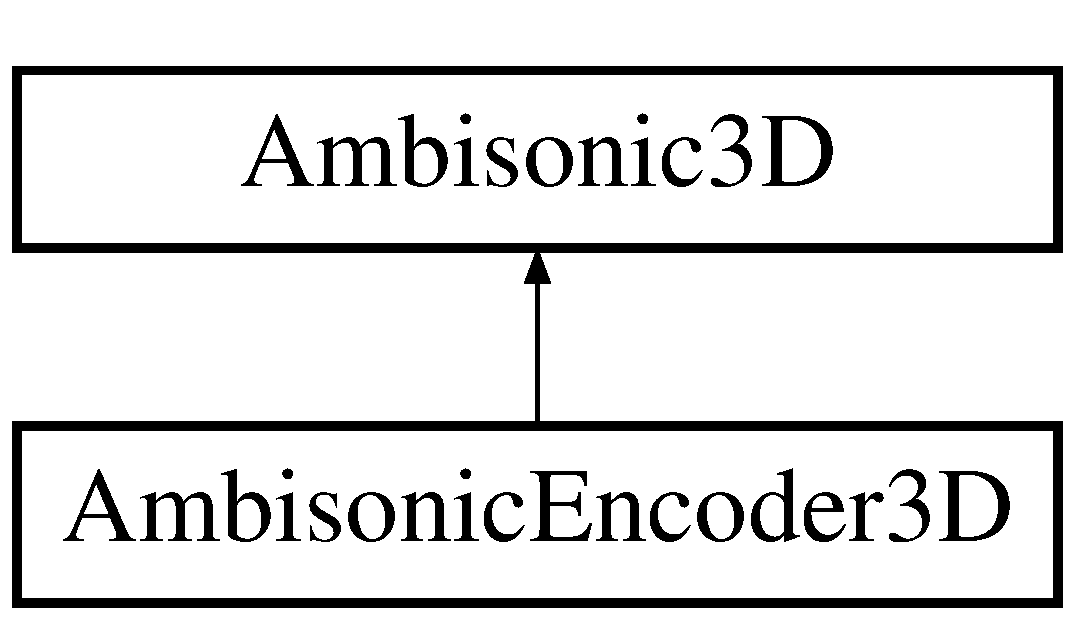
\includegraphics[height=2.000000cm]{class_ambisonic_encoder3_d}
\end{center}
\end{figure}
\subsection*{Public Member Functions}
\begin{DoxyCompactItemize}
\item 
\hyperlink{class_ambisonic_encoder3_d_a34d06da180ce0e7c557dcfb59f921460}{Ambisonic\-Encoder3\-D} (unsigned int order=1)
\item 
\hyperlink{class_ambisonic_encoder3_d_a79bf2dd4be497ed6f12b2509d519d35e}{$\sim$\-Ambisonic\-Encoder3\-D} ()
\item 
void \hyperlink{class_ambisonic_encoder3_d_a9283e59d438b5c50563f538f06c55a4f}{set\-Azimuth} (const float azimuth)
\item 
void \hyperlink{class_ambisonic_encoder3_d_a43e55c6883a55f0b1cee88a4229e8dc3}{set\-Elevation} (const float elevation)
\item 
void \hyperlink{class_ambisonic_encoder3_d_aaf4621c3b6361fc271b1726f09496010}{process} (const float input, float $\ast$outputs)
\end{DoxyCompactItemize}
\subsection*{Additional Inherited Members}


\subsection{Detailed Description}
The ambisonic 3\-D encoder.

The encoder should be used to encode a signal in the spherical harmonics domain depending of an order of decomposition. It allows to control the azimuth and the elevation of the encoding. 

\subsection{Constructor \& Destructor Documentation}
\hypertarget{class_ambisonic_encoder3_d_a34d06da180ce0e7c557dcfb59f921460}{\index{Ambisonic\-Encoder3\-D@{Ambisonic\-Encoder3\-D}!Ambisonic\-Encoder3\-D@{Ambisonic\-Encoder3\-D}}
\index{Ambisonic\-Encoder3\-D@{Ambisonic\-Encoder3\-D}!AmbisonicEncoder3D@{Ambisonic\-Encoder3\-D}}
\subsubsection[{Ambisonic\-Encoder3\-D}]{\setlength{\rightskip}{0pt plus 5cm}Ambisonic\-Encoder3\-D\-::\-Ambisonic\-Encoder3\-D (
\begin{DoxyParamCaption}
\item[{unsigned int}]{order = {\ttfamily 1}}
\end{DoxyParamCaption}
)}}\label{class_ambisonic_encoder3_d_a34d06da180ce0e7c557dcfb59f921460}
\begin{DoxyVerb}The decoder constructor.
\end{DoxyVerb}
 
\begin{DoxyParams}{Parameters}
{\em order} & The order, must be at least 1.\\
\hline
\end{DoxyParams}
\hyperlink{interface_hoa_library}{Hoa\-Library} \-: A High Order Ambisonics Library Copyright (c) 2012-\/2013 Julien Colafrancesco, Pierre Guillot, Eliott Paris, C\-I\-C\-M, Universite Paris-\/8. All rights reserved.

Website \-: \href{http://www.mshparisnord.fr/HoaLibrary/}{\tt http\-://www.\-mshparisnord.\-fr/\-Hoa\-Library/} Contacts \-: \href{mailto:cicm.mshparisnord@gmail.com}{\tt cicm.\-mshparisnord@gmail.\-com}

This file is part of H\-O\-A L\-I\-B\-R\-A\-R\-Y.

H\-O\-A L\-I\-B\-R\-A\-R\-Y is free software\-: you can redistribute it and/or modify it under the terms of the G\-N\-U General Public License as published by the Free Software Foundation, either version 3 of the License, or (at your option) any later version.

This program is distributed in the hope that it will be useful, but W\-I\-T\-H\-O\-U\-T A\-N\-Y W\-A\-R\-R\-A\-N\-T\-Y; without even the implied warranty of M\-E\-R\-C\-H\-A\-N\-T\-A\-B\-I\-L\-I\-T\-Y or F\-I\-T\-N\-E\-S\-S F\-O\-R A P\-A\-R\-T\-I\-C\-U\-L\-A\-R P\-U\-R\-P\-O\-S\-E. See the G\-N\-U General Public License for more details.

You should have received a copy of the G\-N\-U General Public License along with this program. If not, see \href{http://www.gnu.org/licenses/}{\tt http\-://www.\-gnu.\-org/licenses/}. \hypertarget{class_ambisonic_encoder3_d_a79bf2dd4be497ed6f12b2509d519d35e}{\index{Ambisonic\-Encoder3\-D@{Ambisonic\-Encoder3\-D}!$\sim$\-Ambisonic\-Encoder3\-D@{$\sim$\-Ambisonic\-Encoder3\-D}}
\index{$\sim$\-Ambisonic\-Encoder3\-D@{$\sim$\-Ambisonic\-Encoder3\-D}!AmbisonicEncoder3D@{Ambisonic\-Encoder3\-D}}
\subsubsection[{$\sim$\-Ambisonic\-Encoder3\-D}]{\setlength{\rightskip}{0pt plus 5cm}Ambisonic\-Encoder3\-D\-::$\sim$\-Ambisonic\-Encoder3\-D (
\begin{DoxyParamCaption}
{}
\end{DoxyParamCaption}
)}}\label{class_ambisonic_encoder3_d_a79bf2dd4be497ed6f12b2509d519d35e}
The decoder destructor. 

\subsection{Member Function Documentation}
\hypertarget{class_ambisonic_encoder3_d_aaf4621c3b6361fc271b1726f09496010}{\index{Ambisonic\-Encoder3\-D@{Ambisonic\-Encoder3\-D}!process@{process}}
\index{process@{process}!AmbisonicEncoder3D@{Ambisonic\-Encoder3\-D}}
\subsubsection[{process}]{\setlength{\rightskip}{0pt plus 5cm}void Ambisonic\-Encoder3\-D\-::process (
\begin{DoxyParamCaption}
\item[{const float}]{input, }
\item[{float $\ast$}]{outputs}
\end{DoxyParamCaption}
)}}\label{class_ambisonic_encoder3_d_aaf4621c3b6361fc271b1726f09496010}
\begin{DoxyVerb}This method compute the encoding.
\end{DoxyVerb}
 
\begin{DoxyParams}{Parameters}
{\em input} & The input sample. \\
\hline
{\em outputs} & The output array that contains the spherical harmonics samples. \\
\hline
\end{DoxyParams}
\hypertarget{class_ambisonic_encoder3_d_a9283e59d438b5c50563f538f06c55a4f}{\index{Ambisonic\-Encoder3\-D@{Ambisonic\-Encoder3\-D}!set\-Azimuth@{set\-Azimuth}}
\index{set\-Azimuth@{set\-Azimuth}!AmbisonicEncoder3D@{Ambisonic\-Encoder3\-D}}
\subsubsection[{set\-Azimuth}]{\setlength{\rightskip}{0pt plus 5cm}void Ambisonic\-Encoder3\-D\-::set\-Azimuth (
\begin{DoxyParamCaption}
\item[{const float}]{azimuth}
\end{DoxyParamCaption}
)}}\label{class_ambisonic_encoder3_d_a9283e59d438b5c50563f538f06c55a4f}
\begin{DoxyVerb}This method set the angle of azimuth.
\end{DoxyVerb}
 
\begin{DoxyParams}{Parameters}
{\em azimuth} & The azimuth in radian, you should prefer to use it between 0 and 2 Pi. \\
\hline
\end{DoxyParams}
\hypertarget{class_ambisonic_encoder3_d_a43e55c6883a55f0b1cee88a4229e8dc3}{\index{Ambisonic\-Encoder3\-D@{Ambisonic\-Encoder3\-D}!set\-Elevation@{set\-Elevation}}
\index{set\-Elevation@{set\-Elevation}!AmbisonicEncoder3D@{Ambisonic\-Encoder3\-D}}
\subsubsection[{set\-Elevation}]{\setlength{\rightskip}{0pt plus 5cm}void Ambisonic\-Encoder3\-D\-::set\-Elevation (
\begin{DoxyParamCaption}
\item[{const float}]{elevation}
\end{DoxyParamCaption}
)}}\label{class_ambisonic_encoder3_d_a43e55c6883a55f0b1cee88a4229e8dc3}
\begin{DoxyVerb}This method set the angle of elevation.
\end{DoxyVerb}
 
\begin{DoxyParams}{Parameters}
{\em azimuth} & The elevation in radian, you should prefer to use it between 0 and 2 Pi. \\
\hline
\end{DoxyParams}


The documentation for this class was generated from the following files\-:\begin{DoxyCompactItemize}
\item 
/\-Users/\-Pierre/\-Source\-Tree/\-Hoa\-Library/\-Sources/hoa\-Encoder/Ambisonic\-Encoder3\-D.\-h\item 
/\-Users/\-Pierre/\-Source\-Tree/\-Hoa\-Library/\-Sources/hoa\-Encoder/Ambisonic\-Encoder3\-D.\-cpp\end{DoxyCompactItemize}

\hypertarget{class_ambisonic_freeverb}{\section{Ambisonic\-Freeverb Class Reference}
\label{class_ambisonic_freeverb}\index{Ambisonic\-Freeverb@{Ambisonic\-Freeverb}}
}


{\ttfamily \#include $<$Ambisonic\-Freeverb.\-h$>$}

Inheritance diagram for Ambisonic\-Freeverb\-:\begin{figure}[H]
\begin{center}
\leavevmode
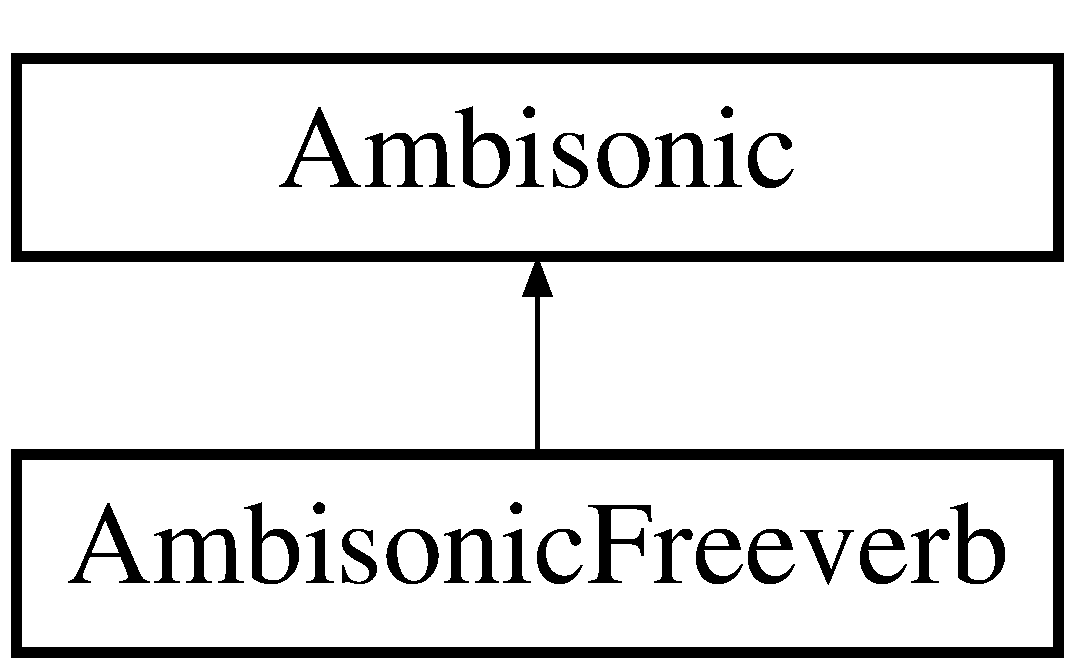
\includegraphics[height=2.000000cm]{class_ambisonic_freeverb}
\end{center}
\end{figure}
\subsection*{Public Member Functions}
\begin{DoxyCompactItemize}
\item 
\hyperlink{class_ambisonic_freeverb_a802c9cbbd9eb3a1d8dbf70205f26807f}{Ambisonic\-Freeverb} (long an\-Order=1, long a\-Vector\-Size=0, double a\-Sampling\-Rate=44100.)
\item 
\hypertarget{class_ambisonic_freeverb_aa242daed003879c71050d63cc4188195}{void {\bfseries set\-Vector\-Size} (long a\-Vector\-Size)}\label{class_ambisonic_freeverb_aa242daed003879c71050d63cc4188195}

\item 
\hypertarget{class_ambisonic_freeverb_a62301fda369160aa580f6273db539055}{void {\bfseries set\-Sampling\-Rate} (long a\-Sampling\-Rate)}\label{class_ambisonic_freeverb_a62301fda369160aa580f6273db539055}

\item 
\hypertarget{class_ambisonic_freeverb_a065b4ef4d872581db86785c4bcc3dcc2}{void {\bfseries set\-Dry\-Value} (double value)}\label{class_ambisonic_freeverb_a065b4ef4d872581db86785c4bcc3dcc2}

\item 
\hypertarget{class_ambisonic_freeverb_a9da2b23831a4481687a8dc75340ccd98}{double {\bfseries get\-Dry\-Value} ()}\label{class_ambisonic_freeverb_a9da2b23831a4481687a8dc75340ccd98}

\item 
\hypertarget{class_ambisonic_freeverb_aeeb92561e55803464be84d97fe689e89}{void {\bfseries set\-Wet\-Value} (double value)}\label{class_ambisonic_freeverb_aeeb92561e55803464be84d97fe689e89}

\item 
\hypertarget{class_ambisonic_freeverb_ada5d7c30656ec0dc98f29b904cf977f8}{double {\bfseries get\-Wet\-Value} ()}\label{class_ambisonic_freeverb_ada5d7c30656ec0dc98f29b904cf977f8}

\item 
\hypertarget{class_ambisonic_freeverb_a5b2485989bf1849e3bbad0d1cb9af6f8}{void {\bfseries setroomsize} (double value)}\label{class_ambisonic_freeverb_a5b2485989bf1849e3bbad0d1cb9af6f8}

\item 
\hypertarget{class_ambisonic_freeverb_aaadead293d132f753b7367fc84d7c8bc}{double {\bfseries getroomsize} ()}\label{class_ambisonic_freeverb_aaadead293d132f753b7367fc84d7c8bc}

\item 
\hypertarget{class_ambisonic_freeverb_aebddbbfa331b9de3025fc714a514b8f4}{void {\bfseries setdamp} (double value)}\label{class_ambisonic_freeverb_aebddbbfa331b9de3025fc714a514b8f4}

\item 
\hypertarget{class_ambisonic_freeverb_a8d52d94300b878036f47a9111c0db53d}{double {\bfseries getdamp} ()}\label{class_ambisonic_freeverb_a8d52d94300b878036f47a9111c0db53d}

\item 
\hypertarget{class_ambisonic_freeverb_a3b08b247c1f5f3207484e80a8a1f79e9}{void {\bfseries setmode} (double value)}\label{class_ambisonic_freeverb_a3b08b247c1f5f3207484e80a8a1f79e9}

\item 
\hypertarget{class_ambisonic_freeverb_a8c5d6630840a73c60880e2dbee5f22dc}{double {\bfseries getmode} ()}\label{class_ambisonic_freeverb_a8c5d6630840a73c60880e2dbee5f22dc}

\item 
\hypertarget{class_ambisonic_freeverb_a16c067aa3294b44ec9ff865dd01ce72c}{void {\bfseries set\-Spread} (double value)}\label{class_ambisonic_freeverb_a16c067aa3294b44ec9ff865dd01ce72c}

\item 
\hypertarget{class_ambisonic_freeverb_a42331b8bdc00b679c0a601a7411aebdf}{void {\bfseries set\-Diffuse\-Spread} (double value)}\label{class_ambisonic_freeverb_a42331b8bdc00b679c0a601a7411aebdf}

\item 
\hypertarget{class_ambisonic_freeverb_aac2ae43a5c6d31adc05c1ee08ce022c0}{void {\bfseries set\-Directional\-Spread} (double value)}\label{class_ambisonic_freeverb_aac2ae43a5c6d31adc05c1ee08ce022c0}

\item 
\hypertarget{class_ambisonic_freeverb_a5f11b83ed6a2f2cc907cecabf8df3b31}{double {\bfseries get\-Diffuse\-Spread} ()}\label{class_ambisonic_freeverb_a5f11b83ed6a2f2cc907cecabf8df3b31}

\item 
\hypertarget{class_ambisonic_freeverb_a249b3173e49fb8cb3ad1daf519e97357}{double {\bfseries get\-Directional\-Spread} ()}\label{class_ambisonic_freeverb_a249b3173e49fb8cb3ad1daf519e97357}

\item 
\hypertarget{class_ambisonic_freeverb_a15cfb9234ddc3661497a9806650f03f2}{void {\bfseries process} (const float $\ast$inputs, float $\ast$outputs)}\label{class_ambisonic_freeverb_a15cfb9234ddc3661497a9806650f03f2}

\item 
\hypertarget{class_ambisonic_freeverb_a3bf00717d5692d2ef26cfa0e83001b63}{void {\bfseries process} (const double $\ast$inputs, double $\ast$outputs)}\label{class_ambisonic_freeverb_a3bf00717d5692d2ef26cfa0e83001b63}

\item 
\hypertarget{class_ambisonic_freeverb_a2f9bf07f2091071471f2f6803fd31fcb}{void {\bfseries process} (float $\ast$io\-Vectors)}\label{class_ambisonic_freeverb_a2f9bf07f2091071471f2f6803fd31fcb}

\item 
\hypertarget{class_ambisonic_freeverb_a0b1c001c27810780b802a34fe9fd206c}{void {\bfseries process} (double $\ast$io\-Vectors)}\label{class_ambisonic_freeverb_a0b1c001c27810780b802a34fe9fd206c}

\item 
\hypertarget{class_ambisonic_freeverb_acc58d029bd3c3b55cf9a13e2c164fae8}{void {\bfseries process} (const float $\ast$const $\ast$inputs, float $\ast$$\ast$outputs)}\label{class_ambisonic_freeverb_acc58d029bd3c3b55cf9a13e2c164fae8}

\item 
\hypertarget{class_ambisonic_freeverb_ae31f0e933fe2c4c7ab5982a83481a2d3}{void {\bfseries process} (const double $\ast$const $\ast$inputs, double $\ast$$\ast$outputs)}\label{class_ambisonic_freeverb_ae31f0e933fe2c4c7ab5982a83481a2d3}

\item 
\hypertarget{class_ambisonic_freeverb_af73fe573fd3a25e279ab14feb95070c7}{void {\bfseries process} (float $\ast$$\ast$io\-Vectors)}\label{class_ambisonic_freeverb_af73fe573fd3a25e279ab14feb95070c7}

\item 
\hypertarget{class_ambisonic_freeverb_a9e90790840fb793f779a3f2d985fbdfa}{void {\bfseries process} (double $\ast$$\ast$io\-Vectors)}\label{class_ambisonic_freeverb_a9e90790840fb793f779a3f2d985fbdfa}

\end{DoxyCompactItemize}
\subsection*{Additional Inherited Members}


\subsection{Detailed Description}
Hoa\-Library \-: A High Order Ambisonics Library Copyright (c) 2012-\/2013 Julien Colafrancesco, Pierre Guillot, Eliott Paris, C\-I\-C\-M, Universite Paris-\/8. All rights reserved.

Website \-: \href{http://www.mshparisnord.fr/hoalibrary/}{\tt http\-://www.\-mshparisnord.\-fr/hoalibrary/} Contacts \-: \href{mailto:cicm.mshparisnord@gmail.com}{\tt cicm.\-mshparisnord@gmail.\-com}

Redistribution and use in source and binary forms, with or without modification, are permitted provided that the following conditions are met\-:


\begin{DoxyItemize}
\item Redistributions may not be sold, nor may they be used in a commercial product or activity.
\item Redistributions of source code must retain the above copyright notice, this list of conditions and the following disclaimer.
\item Redistributions in binary form must reproduce the above copyright notice, this list of conditions and the following disclaimer in the documentation and/or other materials provided with the distribution.
\item Neither the name of the C\-I\-C\-M nor the names of its contributors may be used to endorse or promote products derived from this software without specific prior written permission.
\end{DoxyItemize}

T\-H\-I\-S S\-O\-F\-T\-W\-A\-R\-E I\-S P\-R\-O\-V\-I\-D\-E\-D B\-Y T\-H\-E C\-O\-P\-Y\-R\-I\-G\-H\-T H\-O\-L\-D\-E\-R\-S A\-N\-D C\-O\-N\-T\-R\-I\-B\-U\-T\-O\-R\-S \char`\"{}\-A\-S I\-S\char`\"{} A\-N\-D A\-N\-Y E\-X\-P\-R\-E\-S\-S O\-R I\-M\-P\-L\-I\-E\-D W\-A\-R\-R\-A\-N\-T\-I\-E\-S, I\-N\-C\-L\-U\-D\-I\-N\-G, B\-U\-T N\-O\-T L\-I\-M\-I\-T\-E\-D T\-O, T\-H\-E I\-M\-P\-L\-I\-E\-D W\-A\-R\-R\-A\-N\-T\-I\-E\-S O\-F M\-E\-R\-C\-H\-A\-N\-T\-A\-B\-I\-L\-I\-T\-Y A\-N\-D F\-I\-T\-N\-E\-S\-S F\-O\-R A P\-A\-R\-T\-I\-C\-U\-L\-A\-R P\-U\-R\-P\-O\-S\-E A\-R\-E D\-I\-S\-C\-L\-A\-I\-M\-E\-D. I\-N N\-O E\-V\-E\-N\-T S\-H\-A\-L\-L T\-H\-E C\-O\-P\-Y\-R\-I\-G\-H\-T H\-O\-L\-D\-E\-R O\-R C\-O\-N\-T\-R\-I\-B\-U\-T\-O\-R\-S B\-E L\-I\-A\-B\-L\-E F\-O\-R A\-N\-Y D\-I\-R\-E\-C\-T, I\-N\-D\-I\-R\-E\-C\-T, I\-N\-C\-I\-D\-E\-N\-T\-A\-L, S\-P\-E\-C\-I\-A\-L, E\-X\-E\-M\-P\-L\-A\-R\-Y, O\-R C\-O\-N\-S\-E\-Q\-U\-E\-N\-T\-I\-A\-L D\-A\-M\-A\-G\-E\-S (I\-N\-C\-L\-U\-D\-I\-N\-G, B\-U\-T N\-O\-T L\-I\-M\-I\-T\-E\-D T\-O, P\-R\-O\-C\-U\-R\-E\-M\-E\-N\-T O\-F S\-U\-B\-S\-T\-I\-T\-U\-T\-E G\-O\-O\-D\-S O\-R S\-E\-R\-V\-I\-C\-E\-S; L\-O\-S\-S O\-F U\-S\-E, D\-A\-T\-A, O\-R P\-R\-O\-F\-I\-T\-S; O\-R B\-U\-S\-I\-N\-E\-S\-S I\-N\-T\-E\-R\-R\-U\-P\-T\-I\-O\-N) H\-O\-W\-E\-V\-E\-R C\-A\-U\-S\-E\-D A\-N\-D O\-N A\-N\-Y T\-H\-E\-O\-R\-Y O\-F L\-I\-A\-B\-I\-L\-I\-T\-Y, W\-H\-E\-T\-H\-E\-R I\-N C\-O\-N\-T\-R\-A\-C\-T, S\-T\-R\-I\-C\-T L\-I\-A\-B\-I\-L\-I\-T\-Y, O\-R T\-O\-R\-T (I\-N\-C\-L\-U\-D\-I\-N\-G N\-E\-G\-L\-I\-G\-E\-N\-C\-E O\-R O\-T\-H\-E\-R\-W\-I\-S\-E) A\-R\-I\-S\-I\-N\-G I\-N A\-N\-Y W\-A\-Y O\-U\-T O\-F T\-H\-E U\-S\-E O\-F T\-H\-I\-S S\-O\-F\-T\-W\-A\-R\-E, E\-V\-E\-N I\-F A\-D\-V\-I\-S\-E\-D O\-F T\-H\-E P\-O\-S\-S\-I\-B\-I\-L\-I\-T\-Y O\-F S\-U\-C\-H D\-A\-M\-A\-G\-E. 

\subsection{Constructor \& Destructor Documentation}
\hypertarget{class_ambisonic_freeverb_a802c9cbbd9eb3a1d8dbf70205f26807f}{\index{Ambisonic\-Freeverb@{Ambisonic\-Freeverb}!Ambisonic\-Freeverb@{Ambisonic\-Freeverb}}
\index{Ambisonic\-Freeverb@{Ambisonic\-Freeverb}!AmbisonicFreeverb@{Ambisonic\-Freeverb}}
\subsubsection[{Ambisonic\-Freeverb}]{\setlength{\rightskip}{0pt plus 5cm}Ambisonic\-Freeverb\-::\-Ambisonic\-Freeverb (
\begin{DoxyParamCaption}
\item[{long}]{an\-Order = {\ttfamily 1}, }
\item[{long}]{a\-Vector\-Size = {\ttfamily 0}, }
\item[{double}]{a\-Sampling\-Rate = {\ttfamily 44100.}}
\end{DoxyParamCaption}
)}}\label{class_ambisonic_freeverb_a802c9cbbd9eb3a1d8dbf70205f26807f}
Hoa\-Library \-: A High Order Ambisonics Library Copyright (c) 2012-\/2013 Julien Colafrancesco, Pierre Guillot, Eliott Paris, C\-I\-C\-M, Universite Paris-\/8. All rights reserved.

Website \-: \href{http://www.mshparisnord.fr/hoalibrary/}{\tt http\-://www.\-mshparisnord.\-fr/hoalibrary/} Contacts \-: \href{mailto:cicm.mshparisnord@gmail.com}{\tt cicm.\-mshparisnord@gmail.\-com}

Redistribution and use in source and binary forms, with or without modification, are permitted provided that the following conditions are met\-:


\begin{DoxyItemize}
\item Redistributions may not be sold, nor may they be used in a commercial product or activity.
\item Redistributions of source code must retain the above copyright notice, this list of conditions and the following disclaimer.
\item Redistributions in binary form must reproduce the above copyright notice, this list of conditions and the following disclaimer in the documentation and/or other materials provided with the distribution.
\item Neither the name of the C\-I\-C\-M nor the names of its contributors may be used to endorse or promote products derived from this software without specific prior written permission.
\end{DoxyItemize}

T\-H\-I\-S S\-O\-F\-T\-W\-A\-R\-E I\-S P\-R\-O\-V\-I\-D\-E\-D B\-Y T\-H\-E C\-O\-P\-Y\-R\-I\-G\-H\-T H\-O\-L\-D\-E\-R\-S A\-N\-D C\-O\-N\-T\-R\-I\-B\-U\-T\-O\-R\-S \char`\"{}\-A\-S I\-S\char`\"{} A\-N\-D A\-N\-Y E\-X\-P\-R\-E\-S\-S O\-R I\-M\-P\-L\-I\-E\-D W\-A\-R\-R\-A\-N\-T\-I\-E\-S, I\-N\-C\-L\-U\-D\-I\-N\-G, B\-U\-T N\-O\-T L\-I\-M\-I\-T\-E\-D T\-O, T\-H\-E I\-M\-P\-L\-I\-E\-D W\-A\-R\-R\-A\-N\-T\-I\-E\-S O\-F M\-E\-R\-C\-H\-A\-N\-T\-A\-B\-I\-L\-I\-T\-Y A\-N\-D F\-I\-T\-N\-E\-S\-S F\-O\-R A P\-A\-R\-T\-I\-C\-U\-L\-A\-R P\-U\-R\-P\-O\-S\-E A\-R\-E D\-I\-S\-C\-L\-A\-I\-M\-E\-D. I\-N N\-O E\-V\-E\-N\-T S\-H\-A\-L\-L T\-H\-E C\-O\-P\-Y\-R\-I\-G\-H\-T H\-O\-L\-D\-E\-R O\-R C\-O\-N\-T\-R\-I\-B\-U\-T\-O\-R\-S B\-E L\-I\-A\-B\-L\-E F\-O\-R A\-N\-Y D\-I\-R\-E\-C\-T, I\-N\-D\-I\-R\-E\-C\-T, I\-N\-C\-I\-D\-E\-N\-T\-A\-L, S\-P\-E\-C\-I\-A\-L, E\-X\-E\-M\-P\-L\-A\-R\-Y, O\-R C\-O\-N\-S\-E\-Q\-U\-E\-N\-T\-I\-A\-L D\-A\-M\-A\-G\-E\-S (I\-N\-C\-L\-U\-D\-I\-N\-G, B\-U\-T N\-O\-T L\-I\-M\-I\-T\-E\-D T\-O, P\-R\-O\-C\-U\-R\-E\-M\-E\-N\-T O\-F S\-U\-B\-S\-T\-I\-T\-U\-T\-E G\-O\-O\-D\-S O\-R S\-E\-R\-V\-I\-C\-E\-S; L\-O\-S\-S O\-F U\-S\-E, D\-A\-T\-A, O\-R P\-R\-O\-F\-I\-T\-S; O\-R B\-U\-S\-I\-N\-E\-S\-S I\-N\-T\-E\-R\-R\-U\-P\-T\-I\-O\-N) H\-O\-W\-E\-V\-E\-R C\-A\-U\-S\-E\-D A\-N\-D O\-N A\-N\-Y T\-H\-E\-O\-R\-Y O\-F L\-I\-A\-B\-I\-L\-I\-T\-Y, W\-H\-E\-T\-H\-E\-R I\-N C\-O\-N\-T\-R\-A\-C\-T, S\-T\-R\-I\-C\-T L\-I\-A\-B\-I\-L\-I\-T\-Y, O\-R T\-O\-R\-T (I\-N\-C\-L\-U\-D\-I\-N\-G N\-E\-G\-L\-I\-G\-E\-N\-C\-E O\-R O\-T\-H\-E\-R\-W\-I\-S\-E) A\-R\-I\-S\-I\-N\-G I\-N A\-N\-Y W\-A\-Y O\-U\-T O\-F T\-H\-E U\-S\-E O\-F T\-H\-I\-S S\-O\-F\-T\-W\-A\-R\-E, E\-V\-E\-N I\-F A\-D\-V\-I\-S\-E\-D O\-F T\-H\-E P\-O\-S\-S\-I\-B\-I\-L\-I\-T\-Y O\-F S\-U\-C\-H D\-A\-M\-A\-G\-E. 

The documentation for this class was generated from the following files\-:\begin{DoxyCompactItemize}
\item 
/\-Users/\-Pierre/\-Source\-Tree/\-Hoa\-Library/\-Sources/hoa\-Freeverb/Ambisonic\-Freeverb.\-h\item 
/\-Users/\-Pierre/\-Source\-Tree/\-Hoa\-Library/\-Sources/hoa\-Freeverb/Ambisonic\-Freeverb.\-cpp\end{DoxyCompactItemize}

\hypertarget{class_ambisonic_map}{\section{Ambisonic\-Map Class Reference}
\label{class_ambisonic_map}\index{Ambisonic\-Map@{Ambisonic\-Map}}
}


{\ttfamily \#include $<$Ambisonic\-Map.\-h$>$}

Inheritance diagram for Ambisonic\-Map\-:\begin{figure}[H]
\begin{center}
\leavevmode
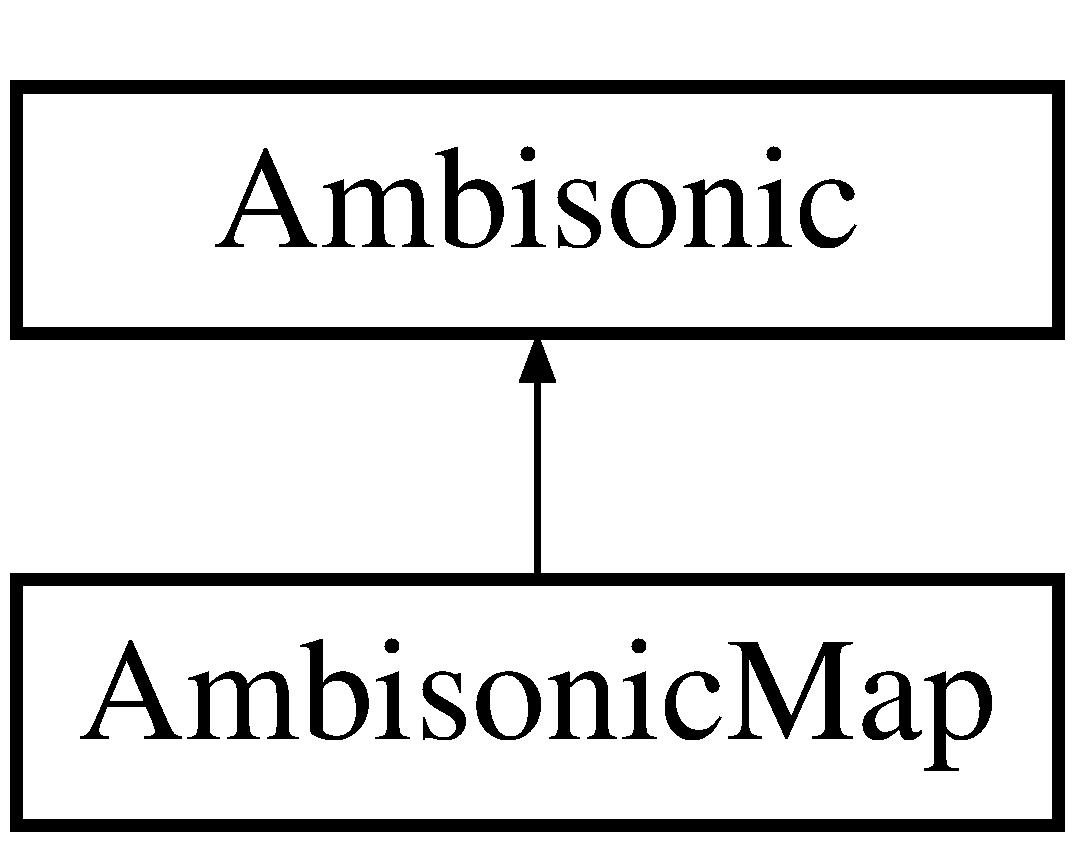
\includegraphics[height=2.000000cm]{class_ambisonic_map}
\end{center}
\end{figure}
\subsection*{Public Member Functions}
\begin{DoxyCompactItemize}
\item 
\hyperlink{class_ambisonic_map_a44db87a2d97aa5851b5fc81be2a33d08}{Ambisonic\-Map} (long an\-Order=1, long a\-Ramp\-Sample=4410, long a\-Vector\-Size=0, long a\-Sampling\-Rate=44100)
\end{DoxyCompactItemize}


\subsection{Detailed Description}
\hyperlink{interface_hoa_library}{Hoa\-Library} \-: A High Order Ambisonics Library Copyright (c) 2012-\/2013 Julien Colafrancesco, Pierre Guillot, Eliott Paris, C\-I\-C\-M, Universite Paris-\/8. All rights reserved.

Website \-: \href{http://www.mshparisnord.fr/hoalibrary/}{\tt http\-://www.\-mshparisnord.\-fr/hoalibrary/} Contacts \-: \href{mailto:cicm.mshparisnord@gmail.com}{\tt cicm.\-mshparisnord@gmail.\-com}

Redistribution and use in source and binary forms, with or without modification, are permitted provided that the following conditions are met\-:


\begin{DoxyItemize}
\item Redistributions may not be sold, nor may they be used in a commercial product or activity.
\item Redistributions of source code must retain the above copyright notice, this list of conditions and the following disclaimer.
\item Redistributions in binary form must reproduce the above copyright notice, this list of conditions and the following disclaimer in the documentation and/or other materials provided with the distribution.
\item Neither the name of the C\-I\-C\-M nor the names of its contributors may be used to endorse or promote products derived from this software without specific prior written permission.
\end{DoxyItemize}

T\-H\-I\-S S\-O\-F\-T\-W\-A\-R\-E I\-S P\-R\-O\-V\-I\-D\-E\-D B\-Y T\-H\-E C\-O\-P\-Y\-R\-I\-G\-H\-T H\-O\-L\-D\-E\-R\-S A\-N\-D C\-O\-N\-T\-R\-I\-B\-U\-T\-O\-R\-S \char`\"{}\-A\-S I\-S\char`\"{} A\-N\-D A\-N\-Y E\-X\-P\-R\-E\-S\-S O\-R I\-M\-P\-L\-I\-E\-D W\-A\-R\-R\-A\-N\-T\-I\-E\-S, I\-N\-C\-L\-U\-D\-I\-N\-G, B\-U\-T N\-O\-T L\-I\-M\-I\-T\-E\-D T\-O, T\-H\-E I\-M\-P\-L\-I\-E\-D W\-A\-R\-R\-A\-N\-T\-I\-E\-S O\-F M\-E\-R\-C\-H\-A\-N\-T\-A\-B\-I\-L\-I\-T\-Y A\-N\-D F\-I\-T\-N\-E\-S\-S F\-O\-R A P\-A\-R\-T\-I\-C\-U\-L\-A\-R P\-U\-R\-P\-O\-S\-E A\-R\-E D\-I\-S\-C\-L\-A\-I\-M\-E\-D. I\-N N\-O E\-V\-E\-N\-T S\-H\-A\-L\-L T\-H\-E C\-O\-P\-Y\-R\-I\-G\-H\-T H\-O\-L\-D\-E\-R O\-R C\-O\-N\-T\-R\-I\-B\-U\-T\-O\-R\-S B\-E L\-I\-A\-B\-L\-E F\-O\-R A\-N\-Y D\-I\-R\-E\-C\-T, I\-N\-D\-I\-R\-E\-C\-T, I\-N\-C\-I\-D\-E\-N\-T\-A\-L, S\-P\-E\-C\-I\-A\-L, E\-X\-E\-M\-P\-L\-A\-R\-Y, O\-R C\-O\-N\-S\-E\-Q\-U\-E\-N\-T\-I\-A\-L D\-A\-M\-A\-G\-E\-S (I\-N\-C\-L\-U\-D\-I\-N\-G, B\-U\-T N\-O\-T L\-I\-M\-I\-T\-E\-D T\-O, P\-R\-O\-C\-U\-R\-E\-M\-E\-N\-T O\-F S\-U\-B\-S\-T\-I\-T\-U\-T\-E G\-O\-O\-D\-S O\-R S\-E\-R\-V\-I\-C\-E\-S; L\-O\-S\-S O\-F U\-S\-E, D\-A\-T\-A, O\-R P\-R\-O\-F\-I\-T\-S; O\-R B\-U\-S\-I\-N\-E\-S\-S I\-N\-T\-E\-R\-R\-U\-P\-T\-I\-O\-N) H\-O\-W\-E\-V\-E\-R C\-A\-U\-S\-E\-D A\-N\-D O\-N A\-N\-Y T\-H\-E\-O\-R\-Y O\-F L\-I\-A\-B\-I\-L\-I\-T\-Y, W\-H\-E\-T\-H\-E\-R I\-N C\-O\-N\-T\-R\-A\-C\-T, S\-T\-R\-I\-C\-T L\-I\-A\-B\-I\-L\-I\-T\-Y, O\-R T\-O\-R\-T (I\-N\-C\-L\-U\-D\-I\-N\-G N\-E\-G\-L\-I\-G\-E\-N\-C\-E O\-R O\-T\-H\-E\-R\-W\-I\-S\-E) A\-R\-I\-S\-I\-N\-G I\-N A\-N\-Y W\-A\-Y O\-U\-T O\-F T\-H\-E U\-S\-E O\-F T\-H\-I\-S S\-O\-F\-T\-W\-A\-R\-E, E\-V\-E\-N I\-F A\-D\-V\-I\-S\-E\-D O\-F T\-H\-E P\-O\-S\-S\-I\-B\-I\-L\-I\-T\-Y O\-F S\-U\-C\-H D\-A\-M\-A\-G\-E. 

Definition at line 33 of file Ambisonic\-Map.\-h.



\subsection{Constructor \& Destructor Documentation}
\hypertarget{class_ambisonic_map_a44db87a2d97aa5851b5fc81be2a33d08}{\index{Ambisonic\-Map@{Ambisonic\-Map}!Ambisonic\-Map@{Ambisonic\-Map}}
\index{Ambisonic\-Map@{Ambisonic\-Map}!AmbisonicMap@{Ambisonic\-Map}}
\subsubsection[{Ambisonic\-Map}]{\setlength{\rightskip}{0pt plus 5cm}Ambisonic\-Map\-::\-Ambisonic\-Map (
\begin{DoxyParamCaption}
\item[{long}]{an\-Order = {\ttfamily 1}, }
\item[{long}]{a\-Ramp\-Sample = {\ttfamily 4410}, }
\item[{long}]{a\-Vector\-Size = {\ttfamily 0}, }
\item[{long}]{a\-Sampling\-Rate = {\ttfamily 44100}}
\end{DoxyParamCaption}
)}}\label{class_ambisonic_map_a44db87a2d97aa5851b5fc81be2a33d08}
\hyperlink{interface_hoa_library}{Hoa\-Library} \-: A High Order Ambisonics Library Copyright (c) 2012-\/2013 Julien Colafrancesco, Pierre Guillot, Eliott Paris, C\-I\-C\-M, Universite Paris-\/8. All rights reserved.

Website \-: \href{http://www.mshparisnord.fr/hoalibrary/}{\tt http\-://www.\-mshparisnord.\-fr/hoalibrary/} Contacts \-: \href{mailto:cicm.mshparisnord@gmail.com}{\tt cicm.\-mshparisnord@gmail.\-com}

Redistribution and use in source and binary forms, with or without modification, are permitted provided that the following conditions are met\-:


\begin{DoxyItemize}
\item Redistributions may not be sold, nor may they be used in a commercial product or activity.
\item Redistributions of source code must retain the above copyright notice, this list of conditions and the following disclaimer.
\item Redistributions in binary form must reproduce the above copyright notice, this list of conditions and the following disclaimer in the documentation and/or other materials provided with the distribution.
\item Neither the name of the C\-I\-C\-M nor the names of its contributors may be used to endorse or promote products derived from this software without specific prior written permission.
\end{DoxyItemize}

T\-H\-I\-S S\-O\-F\-T\-W\-A\-R\-E I\-S P\-R\-O\-V\-I\-D\-E\-D B\-Y T\-H\-E C\-O\-P\-Y\-R\-I\-G\-H\-T H\-O\-L\-D\-E\-R\-S A\-N\-D C\-O\-N\-T\-R\-I\-B\-U\-T\-O\-R\-S \char`\"{}\-A\-S I\-S\char`\"{} A\-N\-D A\-N\-Y E\-X\-P\-R\-E\-S\-S O\-R I\-M\-P\-L\-I\-E\-D W\-A\-R\-R\-A\-N\-T\-I\-E\-S, I\-N\-C\-L\-U\-D\-I\-N\-G, B\-U\-T N\-O\-T L\-I\-M\-I\-T\-E\-D T\-O, T\-H\-E I\-M\-P\-L\-I\-E\-D W\-A\-R\-R\-A\-N\-T\-I\-E\-S O\-F M\-E\-R\-C\-H\-A\-N\-T\-A\-B\-I\-L\-I\-T\-Y A\-N\-D F\-I\-T\-N\-E\-S\-S F\-O\-R A P\-A\-R\-T\-I\-C\-U\-L\-A\-R P\-U\-R\-P\-O\-S\-E A\-R\-E D\-I\-S\-C\-L\-A\-I\-M\-E\-D. I\-N N\-O E\-V\-E\-N\-T S\-H\-A\-L\-L T\-H\-E C\-O\-P\-Y\-R\-I\-G\-H\-T H\-O\-L\-D\-E\-R O\-R C\-O\-N\-T\-R\-I\-B\-U\-T\-O\-R\-S B\-E L\-I\-A\-B\-L\-E F\-O\-R A\-N\-Y D\-I\-R\-E\-C\-T, I\-N\-D\-I\-R\-E\-C\-T, I\-N\-C\-I\-D\-E\-N\-T\-A\-L, S\-P\-E\-C\-I\-A\-L, E\-X\-E\-M\-P\-L\-A\-R\-Y, O\-R C\-O\-N\-S\-E\-Q\-U\-E\-N\-T\-I\-A\-L D\-A\-M\-A\-G\-E\-S (I\-N\-C\-L\-U\-D\-I\-N\-G, B\-U\-T N\-O\-T L\-I\-M\-I\-T\-E\-D T\-O, P\-R\-O\-C\-U\-R\-E\-M\-E\-N\-T O\-F S\-U\-B\-S\-T\-I\-T\-U\-T\-E G\-O\-O\-D\-S O\-R S\-E\-R\-V\-I\-C\-E\-S; L\-O\-S\-S O\-F U\-S\-E, D\-A\-T\-A, O\-R P\-R\-O\-F\-I\-T\-S; O\-R B\-U\-S\-I\-N\-E\-S\-S I\-N\-T\-E\-R\-R\-U\-P\-T\-I\-O\-N) H\-O\-W\-E\-V\-E\-R C\-A\-U\-S\-E\-D A\-N\-D O\-N A\-N\-Y T\-H\-E\-O\-R\-Y O\-F L\-I\-A\-B\-I\-L\-I\-T\-Y, W\-H\-E\-T\-H\-E\-R I\-N C\-O\-N\-T\-R\-A\-C\-T, S\-T\-R\-I\-C\-T L\-I\-A\-B\-I\-L\-I\-T\-Y, O\-R T\-O\-R\-T (I\-N\-C\-L\-U\-D\-I\-N\-G N\-E\-G\-L\-I\-G\-E\-N\-C\-E O\-R O\-T\-H\-E\-R\-W\-I\-S\-E) A\-R\-I\-S\-I\-N\-G I\-N A\-N\-Y W\-A\-Y O\-U\-T O\-F T\-H\-E U\-S\-E O\-F T\-H\-I\-S S\-O\-F\-T\-W\-A\-R\-E, E\-V\-E\-N I\-F A\-D\-V\-I\-S\-E\-D O\-F T\-H\-E P\-O\-S\-S\-I\-B\-I\-L\-I\-T\-Y O\-F S\-U\-C\-H D\-A\-M\-A\-G\-E. 

Definition at line 28 of file Ambisonic\-Map.\-cpp.



The documentation for this class was generated from the following files\-:\begin{DoxyCompactItemize}
\item 
/\-Users/\-Pierre/\-Source\-Tree/\-Hoa\-Library/\-Sources/hoa\-Map/Ambisonic\-Map.\-h\item 
/\-Users/\-Pierre/\-Source\-Tree/\-Hoa\-Library/\-Sources/hoa\-Map/Ambisonic\-Map.\-cpp\end{DoxyCompactItemize}

\hypertarget{class_ambisonic_one_pole}{\section{Ambisonic\-One\-Pole Class Reference}
\label{class_ambisonic_one_pole}\index{Ambisonic\-One\-Pole@{Ambisonic\-One\-Pole}}
}


\subsection{Detailed Description}


Definition at line 33 of file Cicm\-One\-Pole.\-h.



The documentation for this class was generated from the following files\-:\begin{DoxyCompactItemize}
\item 
/\-Users/\-Pierre/\-Source\-Tree/\-Hoa\-Library/\-Sources/\-Cicm\-Library/\-Cicm\-Filters/Cicm\-One\-Pole.\-h\item 
/\-Users/\-Pierre/\-Source\-Tree/\-Hoa\-Library/\-Sources/\-Cicm\-Library/\-Cicm\-Filters/Cicm\-One\-Pole.\-cpp\end{DoxyCompactItemize}

\hypertarget{class_ambisonic_optim}{\section{Ambisonic\-Optim Class Reference}
\label{class_ambisonic_optim}\index{Ambisonic\-Optim@{Ambisonic\-Optim}}
}
Inheritance diagram for Ambisonic\-Optim\-:\begin{figure}[H]
\begin{center}
\leavevmode
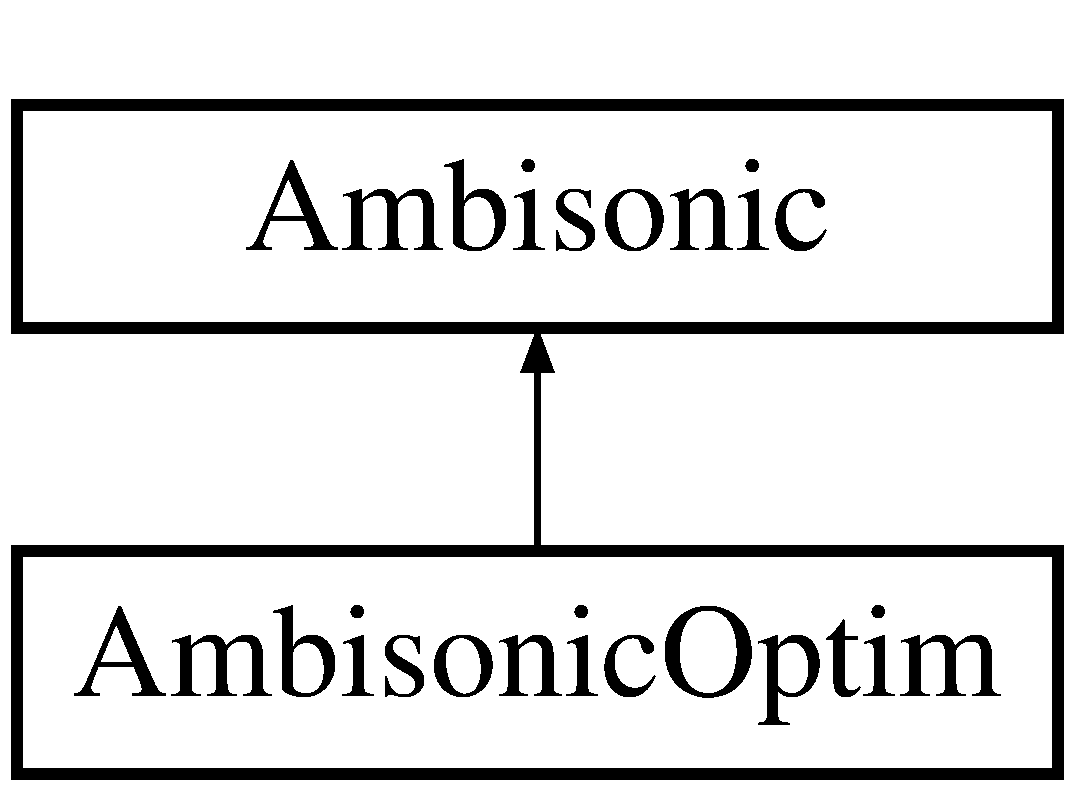
\includegraphics[height=2.000000cm]{class_ambisonic_optim}
\end{center}
\end{figure}
\subsection*{Public Member Functions}
\begin{DoxyCompactItemize}
\item 
\hyperlink{class_ambisonic_optim_adebe5049c799d83f1c936368cf18f5ed}{Ambisonic\-Optim} (long an\-Order=1, long an\-Optim\-Mode=Hoa\-\_\-\-In\-Phase\-\_\-\-Optim, long a\-Vector\-Size=0)
\end{DoxyCompactItemize}


\subsection{Detailed Description}


Definition at line 40 of file Ambisonic\-Optim.\-h.



\subsection{Constructor \& Destructor Documentation}
\hypertarget{class_ambisonic_optim_adebe5049c799d83f1c936368cf18f5ed}{\index{Ambisonic\-Optim@{Ambisonic\-Optim}!Ambisonic\-Optim@{Ambisonic\-Optim}}
\index{Ambisonic\-Optim@{Ambisonic\-Optim}!AmbisonicOptim@{Ambisonic\-Optim}}
\subsubsection[{Ambisonic\-Optim}]{\setlength{\rightskip}{0pt plus 5cm}Ambisonic\-Optim\-::\-Ambisonic\-Optim (
\begin{DoxyParamCaption}
\item[{long}]{an\-Order = {\ttfamily 1}, }
\item[{long}]{an\-Optim\-Mode = {\ttfamily Hoa\-\_\-InPhase\-\_\-Optim}, }
\item[{long}]{a\-Vector\-Size = {\ttfamily 0}}
\end{DoxyParamCaption}
)}}\label{class_ambisonic_optim_adebe5049c799d83f1c936368cf18f5ed}
\hyperlink{interface_hoa_library}{Hoa\-Library} \-: A High Order Ambisonics Library Copyright (c) 2012-\/2013 Julien Colafrancesco, Pierre Guillot, Eliott Paris, C\-I\-C\-M, Universite Paris-\/8. All rights reserved.\-re Guillot, C\-I\-C\-M -\/ Université Paris 8 All rights reserved.

Website \-: \href{http://www.mshparisnord.fr/HoaLibrary/}{\tt http\-://www.\-mshparisnord.\-fr/\-Hoa\-Library/} Contacts \-: \href{mailto:cicm.mshparisnord@gmail.com}{\tt cicm.\-mshparisnord@gmail.\-com}

This file is part of H\-O\-A L\-I\-B\-R\-A\-R\-Y.

H\-O\-A L\-I\-B\-R\-A\-R\-Y is free software\-: you can redistribute it and/or modify it under the terms of the G\-N\-U General Public License as published by the Free Software Foundation, either version 3 of the License, or (at your option) any later version.

This program is distributed in the hope that it will be useful, but W\-I\-T\-H\-O\-U\-T A\-N\-Y W\-A\-R\-R\-A\-N\-T\-Y; without even the implied warranty of M\-E\-R\-C\-H\-A\-N\-T\-A\-B\-I\-L\-I\-T\-Y or F\-I\-T\-N\-E\-S\-S F\-O\-R A P\-A\-R\-T\-I\-C\-U\-L\-A\-R P\-U\-R\-P\-O\-S\-E. See the G\-N\-U General Public License for more details.

You should have received a copy of the G\-N\-U General Public License along with this program. If not, see \href{http://www.gnu.org/licenses/}{\tt http\-://www.\-gnu.\-org/licenses/}. 

Definition at line 29 of file Ambisonic\-Optim.\-cpp.



The documentation for this class was generated from the following files\-:\begin{DoxyCompactItemize}
\item 
/\-Users/\-Pierre/\-Source\-Tree/\-Hoa\-Library/\-Sources/hoa\-Optim/Ambisonic\-Optim.\-h\item 
/\-Users/\-Pierre/\-Source\-Tree/\-Hoa\-Library/\-Sources/hoa\-Optim/Ambisonic\-Optim.\-cpp\end{DoxyCompactItemize}

\hypertarget{class_ambisonic_projector}{\section{Ambisonic\-Projector Class Reference}
\label{class_ambisonic_projector}\index{Ambisonic\-Projector@{Ambisonic\-Projector}}
}


{\ttfamily \#include $<$Ambisonic\-Projector.\-h$>$}

Inheritance diagram for Ambisonic\-Projector\-:\begin{figure}[H]
\begin{center}
\leavevmode
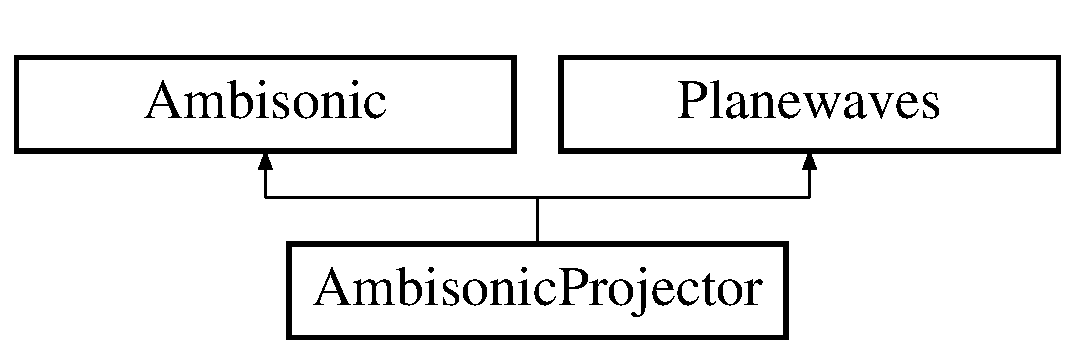
\includegraphics[height=2.000000cm]{class_ambisonic_projector}
\end{center}
\end{figure}
\subsection*{Public Member Functions}
\begin{DoxyCompactItemize}
\item 
\hyperlink{class_ambisonic_projector_a611af47413099ddc30e7075953c9a038}{Ambisonic\-Projector} (long an\-Order=1, long a\-Number\-Of\-Loudspeakers=3, long a\-Vector\-Size=0)
\end{DoxyCompactItemize}


\subsection{Detailed Description}
Hoa\-Library \-: A High Order Ambisonics Library Copyright (c) 2012-\/2013 Julien Colafrancesco, Pierre Guillot, Eliott Paris, C\-I\-C\-M, Universite Paris-\/8. All rights reserved.

Website \-: \href{http://www.mshparisnord.fr/hoalibrary/}{\tt http\-://www.\-mshparisnord.\-fr/hoalibrary/} Contacts \-: \href{mailto:cicm.mshparisnord@gmail.com}{\tt cicm.\-mshparisnord@gmail.\-com}

Redistribution and use in source and binary forms, with or without modification, are permitted provided that the following conditions are met\-:


\begin{DoxyItemize}
\item Redistributions may not be sold, nor may they be used in a commercial product or activity.
\item Redistributions of source code must retain the above copyright notice, this list of conditions and the following disclaimer.
\item Redistributions in binary form must reproduce the above copyright notice, this list of conditions and the following disclaimer in the documentation and/or other materials provided with the distribution.
\item Neither the name of the C\-I\-C\-M nor the names of its contributors may be used to endorse or promote products derived from this software without specific prior written permission.
\end{DoxyItemize}

T\-H\-I\-S S\-O\-F\-T\-W\-A\-R\-E I\-S P\-R\-O\-V\-I\-D\-E\-D B\-Y T\-H\-E C\-O\-P\-Y\-R\-I\-G\-H\-T H\-O\-L\-D\-E\-R\-S A\-N\-D C\-O\-N\-T\-R\-I\-B\-U\-T\-O\-R\-S \char`\"{}\-A\-S I\-S\char`\"{} A\-N\-D A\-N\-Y E\-X\-P\-R\-E\-S\-S O\-R I\-M\-P\-L\-I\-E\-D W\-A\-R\-R\-A\-N\-T\-I\-E\-S, I\-N\-C\-L\-U\-D\-I\-N\-G, B\-U\-T N\-O\-T L\-I\-M\-I\-T\-E\-D T\-O, T\-H\-E I\-M\-P\-L\-I\-E\-D W\-A\-R\-R\-A\-N\-T\-I\-E\-S O\-F M\-E\-R\-C\-H\-A\-N\-T\-A\-B\-I\-L\-I\-T\-Y A\-N\-D F\-I\-T\-N\-E\-S\-S F\-O\-R A P\-A\-R\-T\-I\-C\-U\-L\-A\-R P\-U\-R\-P\-O\-S\-E A\-R\-E D\-I\-S\-C\-L\-A\-I\-M\-E\-D. I\-N N\-O E\-V\-E\-N\-T S\-H\-A\-L\-L T\-H\-E C\-O\-P\-Y\-R\-I\-G\-H\-T H\-O\-L\-D\-E\-R O\-R C\-O\-N\-T\-R\-I\-B\-U\-T\-O\-R\-S B\-E L\-I\-A\-B\-L\-E F\-O\-R A\-N\-Y D\-I\-R\-E\-C\-T, I\-N\-D\-I\-R\-E\-C\-T, I\-N\-C\-I\-D\-E\-N\-T\-A\-L, S\-P\-E\-C\-I\-A\-L, E\-X\-E\-M\-P\-L\-A\-R\-Y, O\-R C\-O\-N\-S\-E\-Q\-U\-E\-N\-T\-I\-A\-L D\-A\-M\-A\-G\-E\-S (I\-N\-C\-L\-U\-D\-I\-N\-G, B\-U\-T N\-O\-T L\-I\-M\-I\-T\-E\-D T\-O, P\-R\-O\-C\-U\-R\-E\-M\-E\-N\-T O\-F S\-U\-B\-S\-T\-I\-T\-U\-T\-E G\-O\-O\-D\-S O\-R S\-E\-R\-V\-I\-C\-E\-S; L\-O\-S\-S O\-F U\-S\-E, D\-A\-T\-A, O\-R P\-R\-O\-F\-I\-T\-S; O\-R B\-U\-S\-I\-N\-E\-S\-S I\-N\-T\-E\-R\-R\-U\-P\-T\-I\-O\-N) H\-O\-W\-E\-V\-E\-R C\-A\-U\-S\-E\-D A\-N\-D O\-N A\-N\-Y T\-H\-E\-O\-R\-Y O\-F L\-I\-A\-B\-I\-L\-I\-T\-Y, W\-H\-E\-T\-H\-E\-R I\-N C\-O\-N\-T\-R\-A\-C\-T, S\-T\-R\-I\-C\-T L\-I\-A\-B\-I\-L\-I\-T\-Y, O\-R T\-O\-R\-T (I\-N\-C\-L\-U\-D\-I\-N\-G N\-E\-G\-L\-I\-G\-E\-N\-C\-E O\-R O\-T\-H\-E\-R\-W\-I\-S\-E) A\-R\-I\-S\-I\-N\-G I\-N A\-N\-Y W\-A\-Y O\-U\-T O\-F T\-H\-E U\-S\-E O\-F T\-H\-I\-S S\-O\-F\-T\-W\-A\-R\-E, E\-V\-E\-N I\-F A\-D\-V\-I\-S\-E\-D O\-F T\-H\-E P\-O\-S\-S\-I\-B\-I\-L\-I\-T\-Y O\-F S\-U\-C\-H D\-A\-M\-A\-G\-E. 

Definition at line 32 of file Ambisonic\-Projector.\-h.



\subsection{Constructor \& Destructor Documentation}
\hypertarget{class_ambisonic_projector_a611af47413099ddc30e7075953c9a038}{\index{Ambisonic\-Projector@{Ambisonic\-Projector}!Ambisonic\-Projector@{Ambisonic\-Projector}}
\index{Ambisonic\-Projector@{Ambisonic\-Projector}!AmbisonicProjector@{Ambisonic\-Projector}}
\subsubsection[{Ambisonic\-Projector}]{\setlength{\rightskip}{0pt plus 5cm}Ambisonic\-Projector\-::\-Ambisonic\-Projector (
\begin{DoxyParamCaption}
\item[{long}]{an\-Order = {\ttfamily 1}, }
\item[{long}]{a\-Number\-Of\-Loudspeakers = {\ttfamily 3}, }
\item[{long}]{a\-Vector\-Size = {\ttfamily 0}}
\end{DoxyParamCaption}
)}}\label{class_ambisonic_projector_a611af47413099ddc30e7075953c9a038}
Hoa\-Library \-: A High Order Ambisonics Library Copyright (c) 2012-\/2013 Julien Colafrancesco, Pierre Guillot, Eliott Paris, C\-I\-C\-M, Universite Paris-\/8. All rights reserved.

Website \-: \href{http://www.mshparisnord.fr/hoalibrary/}{\tt http\-://www.\-mshparisnord.\-fr/hoalibrary/} Contacts \-: \href{mailto:cicm.mshparisnord@gmail.com}{\tt cicm.\-mshparisnord@gmail.\-com}

Redistribution and use in source and binary forms, with or without modification, are permitted provided that the following conditions are met\-:


\begin{DoxyItemize}
\item Redistributions may not be sold, nor may they be used in a commercial product or activity.
\item Redistributions of source code must retain the above copyright notice, this list of conditions and the following disclaimer.
\item Redistributions in binary form must reproduce the above copyright notice, this list of conditions and the following disclaimer in the documentation and/or other materials provided with the distribution.
\item Neither the name of the C\-I\-C\-M nor the names of its contributors may be used to endorse or promote products derived from this software without specific prior written permission.
\end{DoxyItemize}

T\-H\-I\-S S\-O\-F\-T\-W\-A\-R\-E I\-S P\-R\-O\-V\-I\-D\-E\-D B\-Y T\-H\-E C\-O\-P\-Y\-R\-I\-G\-H\-T H\-O\-L\-D\-E\-R\-S A\-N\-D C\-O\-N\-T\-R\-I\-B\-U\-T\-O\-R\-S \char`\"{}\-A\-S I\-S\char`\"{} A\-N\-D A\-N\-Y E\-X\-P\-R\-E\-S\-S O\-R I\-M\-P\-L\-I\-E\-D W\-A\-R\-R\-A\-N\-T\-I\-E\-S, I\-N\-C\-L\-U\-D\-I\-N\-G, B\-U\-T N\-O\-T L\-I\-M\-I\-T\-E\-D T\-O, T\-H\-E I\-M\-P\-L\-I\-E\-D W\-A\-R\-R\-A\-N\-T\-I\-E\-S O\-F M\-E\-R\-C\-H\-A\-N\-T\-A\-B\-I\-L\-I\-T\-Y A\-N\-D F\-I\-T\-N\-E\-S\-S F\-O\-R A P\-A\-R\-T\-I\-C\-U\-L\-A\-R P\-U\-R\-P\-O\-S\-E A\-R\-E D\-I\-S\-C\-L\-A\-I\-M\-E\-D. I\-N N\-O E\-V\-E\-N\-T S\-H\-A\-L\-L T\-H\-E C\-O\-P\-Y\-R\-I\-G\-H\-T H\-O\-L\-D\-E\-R O\-R C\-O\-N\-T\-R\-I\-B\-U\-T\-O\-R\-S B\-E L\-I\-A\-B\-L\-E F\-O\-R A\-N\-Y D\-I\-R\-E\-C\-T, I\-N\-D\-I\-R\-E\-C\-T, I\-N\-C\-I\-D\-E\-N\-T\-A\-L, S\-P\-E\-C\-I\-A\-L, E\-X\-E\-M\-P\-L\-A\-R\-Y, O\-R C\-O\-N\-S\-E\-Q\-U\-E\-N\-T\-I\-A\-L D\-A\-M\-A\-G\-E\-S (I\-N\-C\-L\-U\-D\-I\-N\-G, B\-U\-T N\-O\-T L\-I\-M\-I\-T\-E\-D T\-O, P\-R\-O\-C\-U\-R\-E\-M\-E\-N\-T O\-F S\-U\-B\-S\-T\-I\-T\-U\-T\-E G\-O\-O\-D\-S O\-R S\-E\-R\-V\-I\-C\-E\-S; L\-O\-S\-S O\-F U\-S\-E, D\-A\-T\-A, O\-R P\-R\-O\-F\-I\-T\-S; O\-R B\-U\-S\-I\-N\-E\-S\-S I\-N\-T\-E\-R\-R\-U\-P\-T\-I\-O\-N) H\-O\-W\-E\-V\-E\-R C\-A\-U\-S\-E\-D A\-N\-D O\-N A\-N\-Y T\-H\-E\-O\-R\-Y O\-F L\-I\-A\-B\-I\-L\-I\-T\-Y, W\-H\-E\-T\-H\-E\-R I\-N C\-O\-N\-T\-R\-A\-C\-T, S\-T\-R\-I\-C\-T L\-I\-A\-B\-I\-L\-I\-T\-Y, O\-R T\-O\-R\-T (I\-N\-C\-L\-U\-D\-I\-N\-G N\-E\-G\-L\-I\-G\-E\-N\-C\-E O\-R O\-T\-H\-E\-R\-W\-I\-S\-E) A\-R\-I\-S\-I\-N\-G I\-N A\-N\-Y W\-A\-Y O\-U\-T O\-F T\-H\-E U\-S\-E O\-F T\-H\-I\-S S\-O\-F\-T\-W\-A\-R\-E, E\-V\-E\-N I\-F A\-D\-V\-I\-S\-E\-D O\-F T\-H\-E P\-O\-S\-S\-I\-B\-I\-L\-I\-T\-Y O\-F S\-U\-C\-H D\-A\-M\-A\-G\-E. 

Definition at line 28 of file Ambisonic\-Projector.\-cpp.



The documentation for this class was generated from the following files\-:\begin{DoxyCompactItemize}
\item 
/\-Users/elioton/\-Documents/programmation/\-C\-I\-C\-M/source\-Tree/\-Hoa\-Library/\-Sources/hoa\-Projector/Ambisonic\-Projector.\-h\item 
/\-Users/elioton/\-Documents/programmation/\-C\-I\-C\-M/source\-Tree/\-Hoa\-Library/\-Sources/hoa\-Projector/Ambisonic\-Projector.\-cpp\end{DoxyCompactItemize}

\hypertarget{class_ambisonic_recomposer}{\section{Ambisonic\-Recomposer Class Reference}
\label{class_ambisonic_recomposer}\index{Ambisonic\-Recomposer@{Ambisonic\-Recomposer}}
}
Inheritance diagram for Ambisonic\-Recomposer\-:\begin{figure}[H]
\begin{center}
\leavevmode
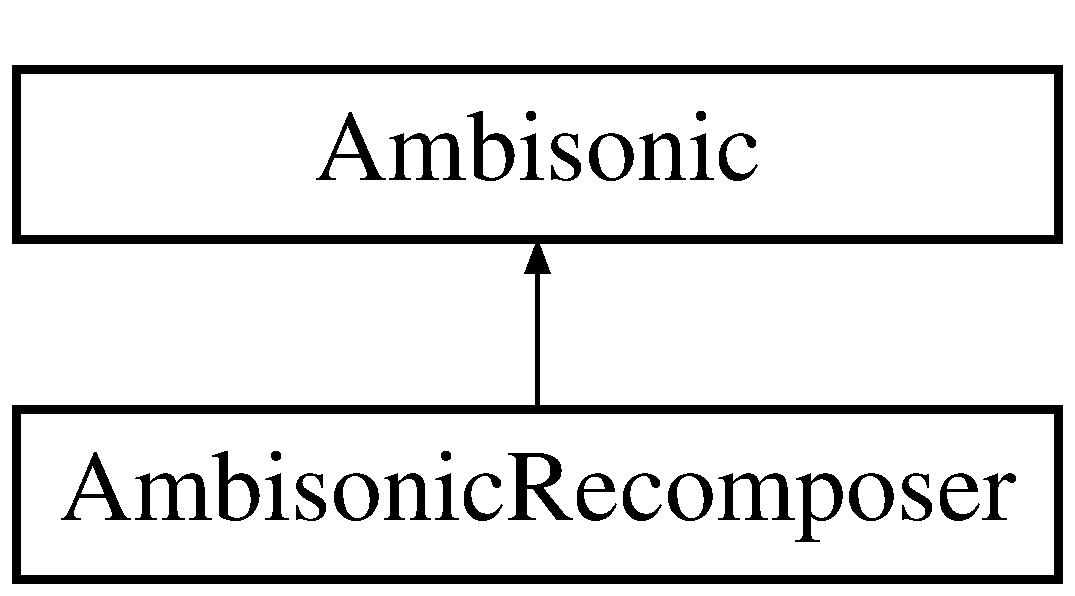
\includegraphics[height=2.000000cm]{class_ambisonic_recomposer}
\end{center}
\end{figure}
\subsection*{Additional Inherited Members}


\subsection{Detailed Description}


Definition at line 42 of file Ambisonic\-Recomposer.\-h.



The documentation for this class was generated from the following files\-:\begin{DoxyCompactItemize}
\item 
/\-Users/\-Pierre/\-Source\-Tree/\-Hoa\-Library/\-Sources/hoa\-Recomposer/Ambisonic\-Recomposer.\-h\item 
/\-Users/\-Pierre/\-Source\-Tree/\-Hoa\-Library/\-Sources/hoa\-Recomposer/Ambisonic\-Recomposer.\-cpp\end{DoxyCompactItemize}

\hypertarget{class_ambisonic_rotate}{\section{Ambisonic\-Rotate Class Reference}
\label{class_ambisonic_rotate}\index{Ambisonic\-Rotate@{Ambisonic\-Rotate}}
}


{\ttfamily \#include $<$Ambisonic\-Rotate.\-h$>$}

Inheritance diagram for Ambisonic\-Rotate\-:\begin{figure}[H]
\begin{center}
\leavevmode
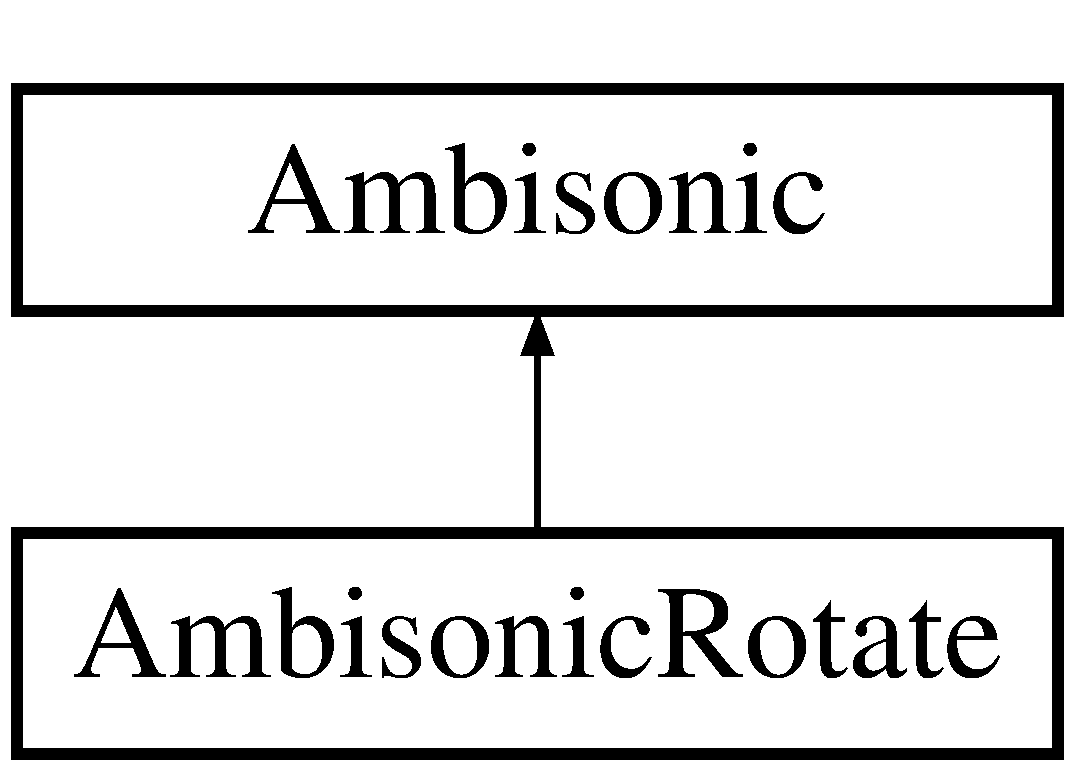
\includegraphics[height=2.000000cm]{class_ambisonic_rotate}
\end{center}
\end{figure}
\subsection*{Public Member Functions}
\begin{DoxyCompactItemize}
\item 
\hyperlink{class_ambisonic_rotate_a27eb54b220b09d45541fb573f295064d}{Ambisonic\-Rotate} (long an\-Order=1, long a\-Vector\-Size=0)
\end{DoxyCompactItemize}


\subsection{Detailed Description}
\hyperlink{interface_hoa_library}{Hoa\-Library} \-: A High Order Ambisonics Library Copyright (c) 2012-\/2013 Julien Colafrancesco, Pierre Guillot, Eliott Paris, C\-I\-C\-M, Universite Paris-\/8. All rights reserved.\-re Guillot, C\-I\-C\-M -\/ Université Paris 8 All rights reserved.

Website \-: \href{http://www.mshparisnord.fr/HoaLibrary/}{\tt http\-://www.\-mshparisnord.\-fr/\-Hoa\-Library/} Contacts \-: \href{mailto:cicm.mshparisnord@gmail.com}{\tt cicm.\-mshparisnord@gmail.\-com}

This file is part of H\-O\-A L\-I\-B\-R\-A\-R\-Y.

H\-O\-A L\-I\-B\-R\-A\-R\-Y is free software\-: you can redistribute it and/or modify it under the terms of the G\-N\-U General Public License as published by the Free Software Foundation, either version 3 of the License, or (at your option) any later version.

This program is distributed in the hope that it will be useful, but W\-I\-T\-H\-O\-U\-T A\-N\-Y W\-A\-R\-R\-A\-N\-T\-Y; without even the implied warranty of M\-E\-R\-C\-H\-A\-N\-T\-A\-B\-I\-L\-I\-T\-Y or F\-I\-T\-N\-E\-S\-S F\-O\-R A P\-A\-R\-T\-I\-C\-U\-L\-A\-R P\-U\-R\-P\-O\-S\-E. See the G\-N\-U General Public License for more details.

You should have received a copy of the G\-N\-U General Public License along with this program. If not, see \href{http://www.gnu.org/licenses/}{\tt http\-://www.\-gnu.\-org/licenses/}. 

\subsection{Constructor \& Destructor Documentation}
\hypertarget{class_ambisonic_rotate_a27eb54b220b09d45541fb573f295064d}{\index{Ambisonic\-Rotate@{Ambisonic\-Rotate}!Ambisonic\-Rotate@{Ambisonic\-Rotate}}
\index{Ambisonic\-Rotate@{Ambisonic\-Rotate}!AmbisonicRotate@{Ambisonic\-Rotate}}
\subsubsection[{Ambisonic\-Rotate}]{\setlength{\rightskip}{0pt plus 5cm}Ambisonic\-Rotate\-::\-Ambisonic\-Rotate (
\begin{DoxyParamCaption}
\item[{long}]{an\-Order = {\ttfamily 1}, }
\item[{long}]{a\-Vector\-Size = {\ttfamily 0}}
\end{DoxyParamCaption}
)}}\label{class_ambisonic_rotate_a27eb54b220b09d45541fb573f295064d}
\hyperlink{interface_hoa_library}{Hoa\-Library} \-: A High Order Ambisonics Library Copyright (c) 2012-\/2013 Julien Colafrancesco, Pierre Guillot, Eliott Paris, C\-I\-C\-M, Universite Paris-\/8. All rights reserved.\-re Guillot, C\-I\-C\-M -\/ Université Paris 8 All rights reserved.

Website \-: \href{http://www.mshparisnord.fr/HoaLibrary/}{\tt http\-://www.\-mshparisnord.\-fr/\-Hoa\-Library/} Contacts \-: \href{mailto:cicm.mshparisnord@gmail.com}{\tt cicm.\-mshparisnord@gmail.\-com}

This file is part of H\-O\-A L\-I\-B\-R\-A\-R\-Y.

H\-O\-A L\-I\-B\-R\-A\-R\-Y is free software\-: you can redistribute it and/or modify it under the terms of the G\-N\-U General Public License as published by the Free Software Foundation, either version 3 of the License, or (at your option) any later version.

This program is distributed in the hope that it will be useful, but W\-I\-T\-H\-O\-U\-T A\-N\-Y W\-A\-R\-R\-A\-N\-T\-Y; without even the implied warranty of M\-E\-R\-C\-H\-A\-N\-T\-A\-B\-I\-L\-I\-T\-Y or F\-I\-T\-N\-E\-S\-S F\-O\-R A P\-A\-R\-T\-I\-C\-U\-L\-A\-R P\-U\-R\-P\-O\-S\-E. See the G\-N\-U General Public License for more details.

You should have received a copy of the G\-N\-U General Public License along with this program. If not, see \href{http://www.gnu.org/licenses/}{\tt http\-://www.\-gnu.\-org/licenses/}. 

The documentation for this class was generated from the following files\-:\begin{DoxyCompactItemize}
\item 
/\-Users/\-Pierre/\-Source\-Tree/\-Hoa\-Library/\-Sources/hoa\-Rotate/Ambisonic\-Rotate.\-h\item 
/\-Users/\-Pierre/\-Source\-Tree/\-Hoa\-Library/\-Sources/hoa\-Rotate/Ambisonic\-Rotate.\-cpp\end{DoxyCompactItemize}

\hypertarget{class_ambisonics_binaural}{\section{Ambisonics\-Binaural Class Reference}
\label{class_ambisonics_binaural}\index{Ambisonics\-Binaural@{Ambisonics\-Binaural}}
}
Inheritance diagram for Ambisonics\-Binaural\-:\begin{figure}[H]
\begin{center}
\leavevmode
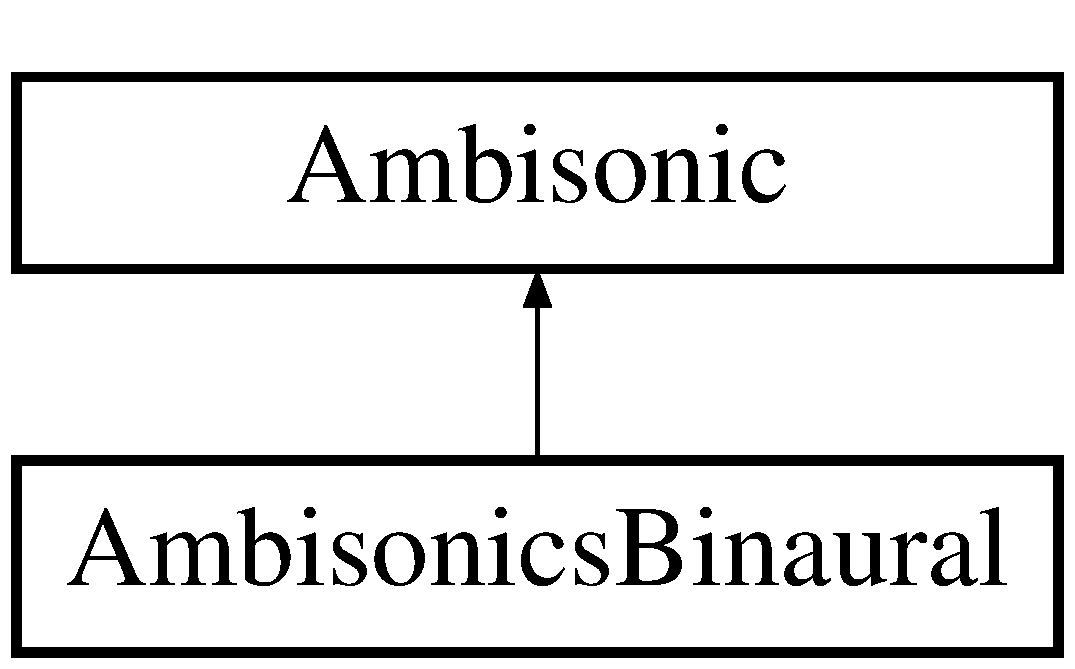
\includegraphics[height=2.000000cm]{class_ambisonics_binaural}
\end{center}
\end{figure}
\subsection*{Public Member Functions}
\begin{DoxyCompactItemize}
\item 
\hyperlink{class_ambisonics_binaural_aa3154f11cb7a385b09a743c5e46ee2e9}{Ambisonics\-Binaural} (long an\-Order=1, std\-::string a\-Root\-Path=\char`\"{}\char`\"{}, long a\-Pinnae\-Size=Hoa\-\_\-\-Small, double a\-Sampling\-Rate=44100, long a\-Vector\-Size=0)
\end{DoxyCompactItemize}


\subsection{Detailed Description}


Definition at line 37 of file Ambisonics\-Binaural.\-h.



\subsection{Constructor \& Destructor Documentation}
\hypertarget{class_ambisonics_binaural_aa3154f11cb7a385b09a743c5e46ee2e9}{\index{Ambisonics\-Binaural@{Ambisonics\-Binaural}!Ambisonics\-Binaural@{Ambisonics\-Binaural}}
\index{Ambisonics\-Binaural@{Ambisonics\-Binaural}!AmbisonicsBinaural@{Ambisonics\-Binaural}}
\subsubsection[{Ambisonics\-Binaural}]{\setlength{\rightskip}{0pt plus 5cm}Ambisonics\-Binaural\-::\-Ambisonics\-Binaural (
\begin{DoxyParamCaption}
\item[{long}]{an\-Order = {\ttfamily 1}, }
\item[{std\-::string}]{a\-Root\-Path = {\ttfamily \char`\"{}\char`\"{}}, }
\item[{long}]{a\-Pinnae\-Size = {\ttfamily Hoa\-\_\-Small}, }
\item[{double}]{a\-Sampling\-Rate = {\ttfamily 44100}, }
\item[{long}]{a\-Vector\-Size = {\ttfamily 0}}
\end{DoxyParamCaption}
)}}\label{class_ambisonics_binaural_aa3154f11cb7a385b09a743c5e46ee2e9}
Hoa\-Library \-: A High Order Ambisonics Library Copyright (c) 2012-\/2013 Julien Colafrancesco, Pierre Guillot, Eliott Paris, C\-I\-C\-M, Universite Paris-\/8. All rights reserved.

Website \-: \href{http://www.mshparisnord.fr/hoalibrary/}{\tt http\-://www.\-mshparisnord.\-fr/hoalibrary/} Contacts \-: \href{mailto:cicm.mshparisnord@gmail.com}{\tt cicm.\-mshparisnord@gmail.\-com}

Redistribution and use in source and binary forms, with or without modification, are permitted provided that the following conditions are met\-:


\begin{DoxyItemize}
\item Redistributions may not be sold, nor may they be used in a commercial product or activity.
\item Redistributions of source code must retain the above copyright notice, this list of conditions and the following disclaimer.
\item Redistributions in binary form must reproduce the above copyright notice, this list of conditions and the following disclaimer in the documentation and/or other materials provided with the distribution.
\item Neither the name of the C\-I\-C\-M nor the names of its contributors may be used to endorse or promote products derived from this software without specific prior written permission.
\end{DoxyItemize}

T\-H\-I\-S S\-O\-F\-T\-W\-A\-R\-E I\-S P\-R\-O\-V\-I\-D\-E\-D B\-Y T\-H\-E C\-O\-P\-Y\-R\-I\-G\-H\-T H\-O\-L\-D\-E\-R\-S A\-N\-D C\-O\-N\-T\-R\-I\-B\-U\-T\-O\-R\-S \char`\"{}\-A\-S I\-S\char`\"{} A\-N\-D A\-N\-Y E\-X\-P\-R\-E\-S\-S O\-R I\-M\-P\-L\-I\-E\-D W\-A\-R\-R\-A\-N\-T\-I\-E\-S, I\-N\-C\-L\-U\-D\-I\-N\-G, B\-U\-T N\-O\-T L\-I\-M\-I\-T\-E\-D T\-O, T\-H\-E I\-M\-P\-L\-I\-E\-D W\-A\-R\-R\-A\-N\-T\-I\-E\-S O\-F M\-E\-R\-C\-H\-A\-N\-T\-A\-B\-I\-L\-I\-T\-Y A\-N\-D F\-I\-T\-N\-E\-S\-S F\-O\-R A P\-A\-R\-T\-I\-C\-U\-L\-A\-R P\-U\-R\-P\-O\-S\-E A\-R\-E D\-I\-S\-C\-L\-A\-I\-M\-E\-D. I\-N N\-O E\-V\-E\-N\-T S\-H\-A\-L\-L T\-H\-E C\-O\-P\-Y\-R\-I\-G\-H\-T H\-O\-L\-D\-E\-R O\-R C\-O\-N\-T\-R\-I\-B\-U\-T\-O\-R\-S B\-E L\-I\-A\-B\-L\-E F\-O\-R A\-N\-Y D\-I\-R\-E\-C\-T, I\-N\-D\-I\-R\-E\-C\-T, I\-N\-C\-I\-D\-E\-N\-T\-A\-L, S\-P\-E\-C\-I\-A\-L, E\-X\-E\-M\-P\-L\-A\-R\-Y, O\-R C\-O\-N\-S\-E\-Q\-U\-E\-N\-T\-I\-A\-L D\-A\-M\-A\-G\-E\-S (I\-N\-C\-L\-U\-D\-I\-N\-G, B\-U\-T N\-O\-T L\-I\-M\-I\-T\-E\-D T\-O, P\-R\-O\-C\-U\-R\-E\-M\-E\-N\-T O\-F S\-U\-B\-S\-T\-I\-T\-U\-T\-E G\-O\-O\-D\-S O\-R S\-E\-R\-V\-I\-C\-E\-S; L\-O\-S\-S O\-F U\-S\-E, D\-A\-T\-A, O\-R P\-R\-O\-F\-I\-T\-S; O\-R B\-U\-S\-I\-N\-E\-S\-S I\-N\-T\-E\-R\-R\-U\-P\-T\-I\-O\-N) H\-O\-W\-E\-V\-E\-R C\-A\-U\-S\-E\-D A\-N\-D O\-N A\-N\-Y T\-H\-E\-O\-R\-Y O\-F L\-I\-A\-B\-I\-L\-I\-T\-Y, W\-H\-E\-T\-H\-E\-R I\-N C\-O\-N\-T\-R\-A\-C\-T, S\-T\-R\-I\-C\-T L\-I\-A\-B\-I\-L\-I\-T\-Y, O\-R T\-O\-R\-T (I\-N\-C\-L\-U\-D\-I\-N\-G N\-E\-G\-L\-I\-G\-E\-N\-C\-E O\-R O\-T\-H\-E\-R\-W\-I\-S\-E) A\-R\-I\-S\-I\-N\-G I\-N A\-N\-Y W\-A\-Y O\-U\-T O\-F T\-H\-E U\-S\-E O\-F T\-H\-I\-S S\-O\-F\-T\-W\-A\-R\-E, E\-V\-E\-N I\-F A\-D\-V\-I\-S\-E\-D O\-F T\-H\-E P\-O\-S\-S\-I\-B\-I\-L\-I\-T\-Y O\-F S\-U\-C\-H D\-A\-M\-A\-G\-E. 

Definition at line 29 of file Ambisonics\-Binaural.\-cpp.



The documentation for this class was generated from the following files\-:\begin{DoxyCompactItemize}
\item 
/\-Users/elioton/\-Documents/programmation/\-C\-I\-C\-M/source\-Tree/\-Hoa\-Library/\-Sources/hoa\-Binaural/Ambisonics\-Binaural.\-h\item 
/\-Users/elioton/\-Documents/programmation/\-C\-I\-C\-M/source\-Tree/\-Hoa\-Library/\-Sources/hoa\-Binaural/Ambisonics\-Binaural.\-cpp\end{DoxyCompactItemize}

\hypertarget{class_ambisonics_decoder}{\section{Ambisonics\-Decoder Class Reference}
\label{class_ambisonics_decoder}\index{Ambisonics\-Decoder@{Ambisonics\-Decoder}}
}


{\ttfamily \#include $<$Ambisonics\-Decoder.\-h$>$}

Inheritance diagram for Ambisonics\-Decoder\-:\begin{figure}[H]
\begin{center}
\leavevmode
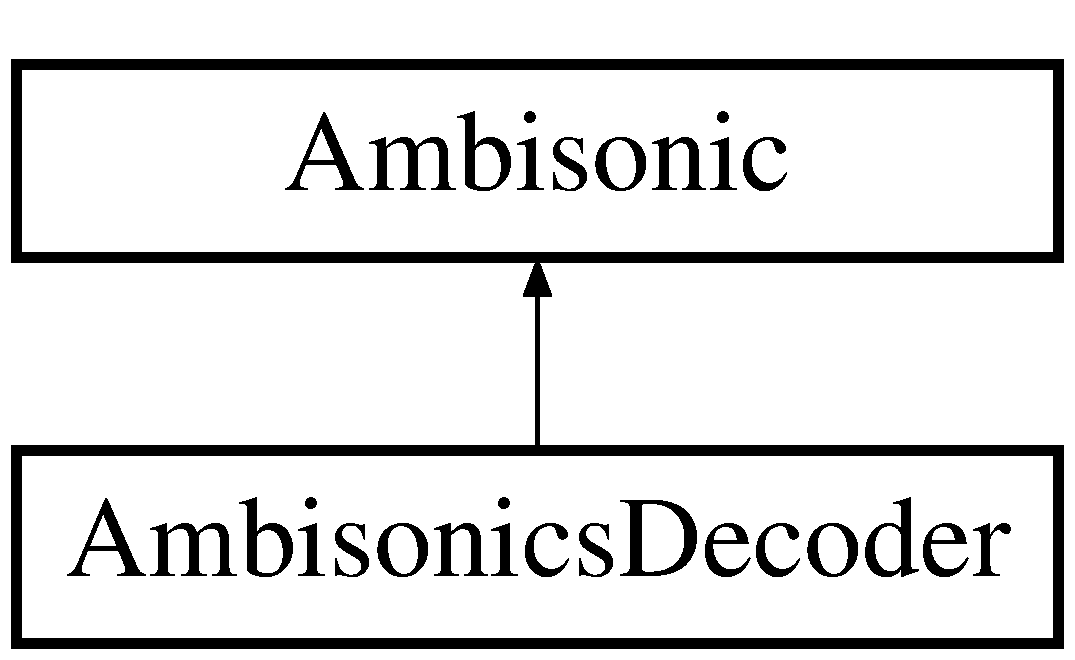
\includegraphics[height=2.000000cm]{class_ambisonics_decoder}
\end{center}
\end{figure}
\subsection*{Public Member Functions}
\begin{DoxyCompactItemize}
\item 
\hyperlink{class_ambisonics_decoder_a45533c94777497b3a01d278f4e04518e}{Ambisonics\-Decoder} (long an\-Order=1, long a\-Number\-Of\-Loudspeakers=0, long a\-Vector\-Size=0)
\end{DoxyCompactItemize}


\subsection{Detailed Description}
Hoa\-Library \-: A High Order Ambisonics Library Copyright (c) 2012-\/2013 Julien Colafrancesco, Pierre Guillot, Eliott Paris, C\-I\-C\-M, Universite Paris-\/8. All rights reserved.

Website \-: \href{http://www.mshparisnord.fr/hoalibrary/}{\tt http\-://www.\-mshparisnord.\-fr/hoalibrary/} Contacts \-: \href{mailto:cicm.mshparisnord@gmail.com}{\tt cicm.\-mshparisnord@gmail.\-com}

Redistribution and use in source and binary forms, with or without modification, are permitted provided that the following conditions are met\-:


\begin{DoxyItemize}
\item Redistributions may not be sold, nor may they be used in a commercial product or activity.
\item Redistributions of source code must retain the above copyright notice, this list of conditions and the following disclaimer.
\item Redistributions in binary form must reproduce the above copyright notice, this list of conditions and the following disclaimer in the documentation and/or other materials provided with the distribution.
\item Neither the name of the C\-I\-C\-M nor the names of its contributors may be used to endorse or promote products derived from this software without specific prior written permission.
\end{DoxyItemize}

T\-H\-I\-S S\-O\-F\-T\-W\-A\-R\-E I\-S P\-R\-O\-V\-I\-D\-E\-D B\-Y T\-H\-E C\-O\-P\-Y\-R\-I\-G\-H\-T H\-O\-L\-D\-E\-R\-S A\-N\-D C\-O\-N\-T\-R\-I\-B\-U\-T\-O\-R\-S \char`\"{}\-A\-S I\-S\char`\"{} A\-N\-D A\-N\-Y E\-X\-P\-R\-E\-S\-S O\-R I\-M\-P\-L\-I\-E\-D W\-A\-R\-R\-A\-N\-T\-I\-E\-S, I\-N\-C\-L\-U\-D\-I\-N\-G, B\-U\-T N\-O\-T L\-I\-M\-I\-T\-E\-D T\-O, T\-H\-E I\-M\-P\-L\-I\-E\-D W\-A\-R\-R\-A\-N\-T\-I\-E\-S O\-F M\-E\-R\-C\-H\-A\-N\-T\-A\-B\-I\-L\-I\-T\-Y A\-N\-D F\-I\-T\-N\-E\-S\-S F\-O\-R A P\-A\-R\-T\-I\-C\-U\-L\-A\-R P\-U\-R\-P\-O\-S\-E A\-R\-E D\-I\-S\-C\-L\-A\-I\-M\-E\-D. I\-N N\-O E\-V\-E\-N\-T S\-H\-A\-L\-L T\-H\-E C\-O\-P\-Y\-R\-I\-G\-H\-T H\-O\-L\-D\-E\-R O\-R C\-O\-N\-T\-R\-I\-B\-U\-T\-O\-R\-S B\-E L\-I\-A\-B\-L\-E F\-O\-R A\-N\-Y D\-I\-R\-E\-C\-T, I\-N\-D\-I\-R\-E\-C\-T, I\-N\-C\-I\-D\-E\-N\-T\-A\-L, S\-P\-E\-C\-I\-A\-L, E\-X\-E\-M\-P\-L\-A\-R\-Y, O\-R C\-O\-N\-S\-E\-Q\-U\-E\-N\-T\-I\-A\-L D\-A\-M\-A\-G\-E\-S (I\-N\-C\-L\-U\-D\-I\-N\-G, B\-U\-T N\-O\-T L\-I\-M\-I\-T\-E\-D T\-O, P\-R\-O\-C\-U\-R\-E\-M\-E\-N\-T O\-F S\-U\-B\-S\-T\-I\-T\-U\-T\-E G\-O\-O\-D\-S O\-R S\-E\-R\-V\-I\-C\-E\-S; L\-O\-S\-S O\-F U\-S\-E, D\-A\-T\-A, O\-R P\-R\-O\-F\-I\-T\-S; O\-R B\-U\-S\-I\-N\-E\-S\-S I\-N\-T\-E\-R\-R\-U\-P\-T\-I\-O\-N) H\-O\-W\-E\-V\-E\-R C\-A\-U\-S\-E\-D A\-N\-D O\-N A\-N\-Y T\-H\-E\-O\-R\-Y O\-F L\-I\-A\-B\-I\-L\-I\-T\-Y, W\-H\-E\-T\-H\-E\-R I\-N C\-O\-N\-T\-R\-A\-C\-T, S\-T\-R\-I\-C\-T L\-I\-A\-B\-I\-L\-I\-T\-Y, O\-R T\-O\-R\-T (I\-N\-C\-L\-U\-D\-I\-N\-G N\-E\-G\-L\-I\-G\-E\-N\-C\-E O\-R O\-T\-H\-E\-R\-W\-I\-S\-E) A\-R\-I\-S\-I\-N\-G I\-N A\-N\-Y W\-A\-Y O\-U\-T O\-F T\-H\-E U\-S\-E O\-F T\-H\-I\-S S\-O\-F\-T\-W\-A\-R\-E, E\-V\-E\-N I\-F A\-D\-V\-I\-S\-E\-D O\-F T\-H\-E P\-O\-S\-S\-I\-B\-I\-L\-I\-T\-Y O\-F S\-U\-C\-H D\-A\-M\-A\-G\-E. 

Definition at line 31 of file Ambisonics\-Decoder.\-h.



\subsection{Constructor \& Destructor Documentation}
\hypertarget{class_ambisonics_decoder_a45533c94777497b3a01d278f4e04518e}{\index{Ambisonics\-Decoder@{Ambisonics\-Decoder}!Ambisonics\-Decoder@{Ambisonics\-Decoder}}
\index{Ambisonics\-Decoder@{Ambisonics\-Decoder}!AmbisonicsDecoder@{Ambisonics\-Decoder}}
\subsubsection[{Ambisonics\-Decoder}]{\setlength{\rightskip}{0pt plus 5cm}Ambisonics\-Decoder\-::\-Ambisonics\-Decoder (
\begin{DoxyParamCaption}
\item[{long}]{an\-Order = {\ttfamily 1}, }
\item[{long}]{a\-Number\-Of\-Loudspeakers = {\ttfamily 0}, }
\item[{long}]{a\-Vector\-Size = {\ttfamily 0}}
\end{DoxyParamCaption}
)}}\label{class_ambisonics_decoder_a45533c94777497b3a01d278f4e04518e}
Hoa\-Library \-: A High Order Ambisonics Library Copyright (c) 2012-\/2013 Julien Colafrancesco, Pierre Guillot, Eliott Paris, C\-I\-C\-M, Universite Paris-\/8. All rights reserved.

Website \-: \href{http://www.mshparisnord.fr/hoalibrary/}{\tt http\-://www.\-mshparisnord.\-fr/hoalibrary/} Contacts \-: \href{mailto:cicm.mshparisnord@gmail.com}{\tt cicm.\-mshparisnord@gmail.\-com}

Redistribution and use in source and binary forms, with or without modification, are permitted provided that the following conditions are met\-:


\begin{DoxyItemize}
\item Redistributions may not be sold, nor may they be used in a commercial product or activity.
\item Redistributions of source code must retain the above copyright notice, this list of conditions and the following disclaimer.
\item Redistributions in binary form must reproduce the above copyright notice, this list of conditions and the following disclaimer in the documentation and/or other materials provided with the distribution.
\item Neither the name of the C\-I\-C\-M nor the names of its contributors may be used to endorse or promote products derived from this software without specific prior written permission.
\end{DoxyItemize}

T\-H\-I\-S S\-O\-F\-T\-W\-A\-R\-E I\-S P\-R\-O\-V\-I\-D\-E\-D B\-Y T\-H\-E C\-O\-P\-Y\-R\-I\-G\-H\-T H\-O\-L\-D\-E\-R\-S A\-N\-D C\-O\-N\-T\-R\-I\-B\-U\-T\-O\-R\-S \char`\"{}\-A\-S I\-S\char`\"{} A\-N\-D A\-N\-Y E\-X\-P\-R\-E\-S\-S O\-R I\-M\-P\-L\-I\-E\-D W\-A\-R\-R\-A\-N\-T\-I\-E\-S, I\-N\-C\-L\-U\-D\-I\-N\-G, B\-U\-T N\-O\-T L\-I\-M\-I\-T\-E\-D T\-O, T\-H\-E I\-M\-P\-L\-I\-E\-D W\-A\-R\-R\-A\-N\-T\-I\-E\-S O\-F M\-E\-R\-C\-H\-A\-N\-T\-A\-B\-I\-L\-I\-T\-Y A\-N\-D F\-I\-T\-N\-E\-S\-S F\-O\-R A P\-A\-R\-T\-I\-C\-U\-L\-A\-R P\-U\-R\-P\-O\-S\-E A\-R\-E D\-I\-S\-C\-L\-A\-I\-M\-E\-D. I\-N N\-O E\-V\-E\-N\-T S\-H\-A\-L\-L T\-H\-E C\-O\-P\-Y\-R\-I\-G\-H\-T H\-O\-L\-D\-E\-R O\-R C\-O\-N\-T\-R\-I\-B\-U\-T\-O\-R\-S B\-E L\-I\-A\-B\-L\-E F\-O\-R A\-N\-Y D\-I\-R\-E\-C\-T, I\-N\-D\-I\-R\-E\-C\-T, I\-N\-C\-I\-D\-E\-N\-T\-A\-L, S\-P\-E\-C\-I\-A\-L, E\-X\-E\-M\-P\-L\-A\-R\-Y, O\-R C\-O\-N\-S\-E\-Q\-U\-E\-N\-T\-I\-A\-L D\-A\-M\-A\-G\-E\-S (I\-N\-C\-L\-U\-D\-I\-N\-G, B\-U\-T N\-O\-T L\-I\-M\-I\-T\-E\-D T\-O, P\-R\-O\-C\-U\-R\-E\-M\-E\-N\-T O\-F S\-U\-B\-S\-T\-I\-T\-U\-T\-E G\-O\-O\-D\-S O\-R S\-E\-R\-V\-I\-C\-E\-S; L\-O\-S\-S O\-F U\-S\-E, D\-A\-T\-A, O\-R P\-R\-O\-F\-I\-T\-S; O\-R B\-U\-S\-I\-N\-E\-S\-S I\-N\-T\-E\-R\-R\-U\-P\-T\-I\-O\-N) H\-O\-W\-E\-V\-E\-R C\-A\-U\-S\-E\-D A\-N\-D O\-N A\-N\-Y T\-H\-E\-O\-R\-Y O\-F L\-I\-A\-B\-I\-L\-I\-T\-Y, W\-H\-E\-T\-H\-E\-R I\-N C\-O\-N\-T\-R\-A\-C\-T, S\-T\-R\-I\-C\-T L\-I\-A\-B\-I\-L\-I\-T\-Y, O\-R T\-O\-R\-T (I\-N\-C\-L\-U\-D\-I\-N\-G N\-E\-G\-L\-I\-G\-E\-N\-C\-E O\-R O\-T\-H\-E\-R\-W\-I\-S\-E) A\-R\-I\-S\-I\-N\-G I\-N A\-N\-Y W\-A\-Y O\-U\-T O\-F T\-H\-E U\-S\-E O\-F T\-H\-I\-S S\-O\-F\-T\-W\-A\-R\-E, E\-V\-E\-N I\-F A\-D\-V\-I\-S\-E\-D O\-F T\-H\-E P\-O\-S\-S\-I\-B\-I\-L\-I\-T\-Y O\-F S\-U\-C\-H D\-A\-M\-A\-G\-E. 

Definition at line 28 of file Ambisonics\-Decoder.\-cpp.



The documentation for this class was generated from the following files\-:\begin{DoxyCompactItemize}
\item 
/\-Users/\-Pierre/\-Source\-Tree/\-Hoa\-Library/\-Sources/hoa\-Decoder/Ambisonics\-Decoder.\-h\item 
/\-Users/\-Pierre/\-Source\-Tree/\-Hoa\-Library/\-Sources/hoa\-Decoder/Ambisonics\-Decoder.\-cpp\end{DoxyCompactItemize}

\hypertarget{class_ambisonics_delay}{\section{Ambisonics\-Delay Class Reference}
\label{class_ambisonics_delay}\index{Ambisonics\-Delay@{Ambisonics\-Delay}}
}


{\ttfamily \#include $<$Ambisonics\-Delay.\-h$>$}

Inheritance diagram for Ambisonics\-Delay\-:\begin{figure}[H]
\begin{center}
\leavevmode
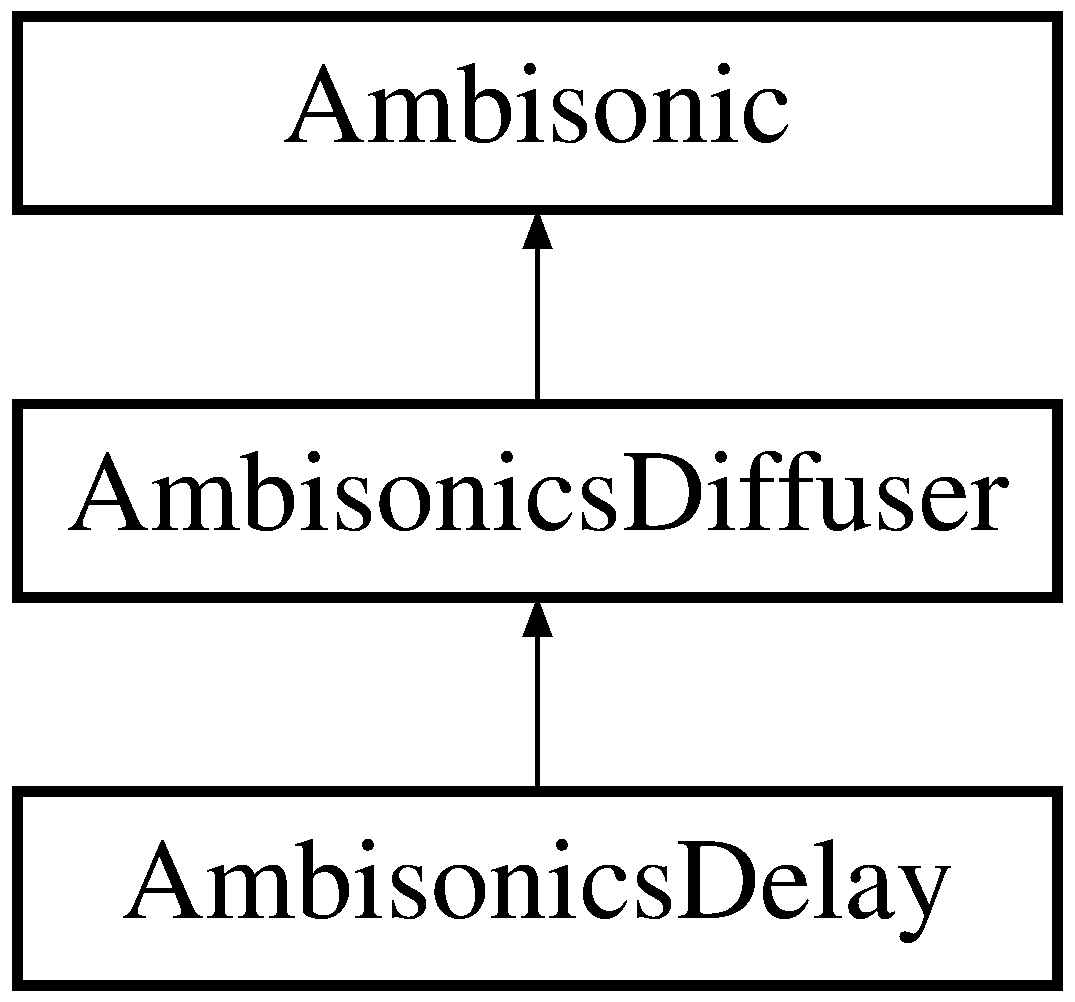
\includegraphics[height=3.000000cm]{class_ambisonics_delay}
\end{center}
\end{figure}
\subsection*{Public Member Functions}
\begin{DoxyCompactItemize}
\item 
\hyperlink{class_ambisonics_delay_ae51a035b03153c0747a6eefba102bdcf}{Ambisonics\-Delay} (long an\-Order=1, bool a\-Mode=Hoa\-\_\-\-Post\-\_\-\-Encoding, double a\-Maximum\-Delay\-In\-Ms=5000., long a\-Vector\-Size=0, long a\-Sampling\-Rate=44100)
\item 
\hypertarget{class_ambisonics_delay_a652ad6ff16b644f267cef3daa662c24f}{void {\bfseries set\-Vector\-Size} (long a\-Vector\-Size)}\label{class_ambisonics_delay_a652ad6ff16b644f267cef3daa662c24f}

\item 
\hypertarget{class_ambisonics_delay_a3e8bb9fe1ebe947f9022946bf9677423}{void {\bfseries set\-Sampling\-Rate} (long a\-Sampling\-Rate)}\label{class_ambisonics_delay_a3e8bb9fe1ebe947f9022946bf9677423}

\item 
\hypertarget{class_ambisonics_delay_a63710b55a6df91212dfbb709dadfc5b6}{void {\bfseries set\-Diffuse\-Factor} (double a\-Diffuse\-Value)}\label{class_ambisonics_delay_a63710b55a6df91212dfbb709dadfc5b6}

\item 
\hypertarget{class_ambisonics_delay_a023a1c68660216fa2359fccab8be8ffb}{void {\bfseries set\-Delay\-Time\-In\-Sample} (long a\-Delay\-In\-Sample)}\label{class_ambisonics_delay_a023a1c68660216fa2359fccab8be8ffb}

\item 
\hypertarget{class_ambisonics_delay_ad8abb0bc0d9b34c857375a5eb6fd5601}{void {\bfseries set\-Delay\-Time\-In\-Ms} (double a\-Delay\-In\-Ms)}\label{class_ambisonics_delay_ad8abb0bc0d9b34c857375a5eb6fd5601}

\item 
\hypertarget{class_ambisonics_delay_ad414fad7d0a4be43e29865b3a2fc9aad}{void {\bfseries set\-Ramp\-In\-Sample} (long a\-Ramp\-In\-Sample)}\label{class_ambisonics_delay_ad414fad7d0a4be43e29865b3a2fc9aad}

\item 
\hypertarget{class_ambisonics_delay_a6dd3696561b8d3b72ab0a016a7b85b81}{void {\bfseries set\-Ramp\-In\-Ms} (double a\-Ramp\-In\-Ms)}\label{class_ambisonics_delay_a6dd3696561b8d3b72ab0a016a7b85b81}

\item 
\hypertarget{class_ambisonics_delay_a5cb44c9bb1e3b93cac70e78d3b2d0c89}{long {\bfseries get\-Delay\-Time\-In\-Sample} ()}\label{class_ambisonics_delay_a5cb44c9bb1e3b93cac70e78d3b2d0c89}

\item 
\hypertarget{class_ambisonics_delay_ad0e480317457a85186ae785bb33832a4}{double {\bfseries get\-Delay\-Time\-In\-Ms} ()}\label{class_ambisonics_delay_ad0e480317457a85186ae785bb33832a4}

\item 
\hypertarget{class_ambisonics_delay_a4bd875e75bf16dfcc043bf95637ca1ed}{long {\bfseries get\-Ramp\-In\-Sample} ()}\label{class_ambisonics_delay_a4bd875e75bf16dfcc043bf95637ca1ed}

\item 
\hypertarget{class_ambisonics_delay_a1e652fc67e8033adfe2ca85e94777dd5}{double {\bfseries get\-Ramp\-In\-Ms} ()}\label{class_ambisonics_delay_a1e652fc67e8033adfe2ca85e94777dd5}

\item 
\hypertarget{class_ambisonics_delay_a689b30eb9bcc242a173326aaa0ef9902}{void {\bfseries process} (double a\-Inputs, double $\ast$a\-Outputs)}\label{class_ambisonics_delay_a689b30eb9bcc242a173326aaa0ef9902}

\item 
\hypertarget{class_ambisonics_delay_a1799746298285eab00432c5d7794bff0}{void {\bfseries process} (double $\ast$a\-Inputs, double $\ast$a\-Outputs)}\label{class_ambisonics_delay_a1799746298285eab00432c5d7794bff0}

\item 
\hypertarget{class_ambisonics_delay_ab1fbab149958d6713a77c8627c17d29a}{void {\bfseries process} (float a\-Inputs, float $\ast$a\-Outputs)}\label{class_ambisonics_delay_ab1fbab149958d6713a77c8627c17d29a}

\item 
\hypertarget{class_ambisonics_delay_ad6d98436f1652d522ef1acfecaea0c8c}{void {\bfseries process} (float $\ast$a\-Inputs, float $\ast$a\-Outputs)}\label{class_ambisonics_delay_ad6d98436f1652d522ef1acfecaea0c8c}

\item 
\hypertarget{class_ambisonics_delay_a3e443751cd4229db04e30375a76116f7}{void {\bfseries process} (double $\ast$a\-Inputs, double $\ast$$\ast$a\-Outputs)}\label{class_ambisonics_delay_a3e443751cd4229db04e30375a76116f7}

\item 
\hypertarget{class_ambisonics_delay_aeb97d99deaac12831fcb093112222594}{void {\bfseries process} (double $\ast$$\ast$a\-Inputs, double $\ast$$\ast$a\-Outputs)}\label{class_ambisonics_delay_aeb97d99deaac12831fcb093112222594}

\item 
\hypertarget{class_ambisonics_delay_a2d3baba33f0ff7e63b77cdded8d3e59b}{void {\bfseries process} (float $\ast$a\-Inputs, float $\ast$$\ast$a\-Outputs)}\label{class_ambisonics_delay_a2d3baba33f0ff7e63b77cdded8d3e59b}

\item 
\hypertarget{class_ambisonics_delay_a77e0021d85260c81457f0dd7216582e6}{void {\bfseries process} (float $\ast$$\ast$a\-Inputs, float $\ast$$\ast$a\-Outputs)}\label{class_ambisonics_delay_a77e0021d85260c81457f0dd7216582e6}

\end{DoxyCompactItemize}
\subsection*{Additional Inherited Members}


\subsection{Detailed Description}
Hoa\-Library \-: A High Order Ambisonics Library Copyright (c) 2012-\/2013 Julien Colafrancesco, Pierre Guillot, Eliott Paris, C\-I\-C\-M, Universite Paris-\/8. All rights reserved.

Website \-: \href{http://www.mshparisnord.fr/hoalibrary/}{\tt http\-://www.\-mshparisnord.\-fr/hoalibrary/} Contacts \-: \href{mailto:cicm.mshparisnord@gmail.com}{\tt cicm.\-mshparisnord@gmail.\-com}

Redistribution and use in source and binary forms, with or without modification, are permitted provided that the following conditions are met\-:


\begin{DoxyItemize}
\item Redistributions may not be sold, nor may they be used in a commercial product or activity.
\item Redistributions of source code must retain the above copyright notice, this list of conditions and the following disclaimer.
\item Redistributions in binary form must reproduce the above copyright notice, this list of conditions and the following disclaimer in the documentation and/or other materials provided with the distribution.
\item Neither the name of the C\-I\-C\-M nor the names of its contributors may be used to endorse or promote products derived from this software without specific prior written permission.
\end{DoxyItemize}

T\-H\-I\-S S\-O\-F\-T\-W\-A\-R\-E I\-S P\-R\-O\-V\-I\-D\-E\-D B\-Y T\-H\-E C\-O\-P\-Y\-R\-I\-G\-H\-T H\-O\-L\-D\-E\-R\-S A\-N\-D C\-O\-N\-T\-R\-I\-B\-U\-T\-O\-R\-S \char`\"{}\-A\-S I\-S\char`\"{} A\-N\-D A\-N\-Y E\-X\-P\-R\-E\-S\-S O\-R I\-M\-P\-L\-I\-E\-D W\-A\-R\-R\-A\-N\-T\-I\-E\-S, I\-N\-C\-L\-U\-D\-I\-N\-G, B\-U\-T N\-O\-T L\-I\-M\-I\-T\-E\-D T\-O, T\-H\-E I\-M\-P\-L\-I\-E\-D W\-A\-R\-R\-A\-N\-T\-I\-E\-S O\-F M\-E\-R\-C\-H\-A\-N\-T\-A\-B\-I\-L\-I\-T\-Y A\-N\-D F\-I\-T\-N\-E\-S\-S F\-O\-R A P\-A\-R\-T\-I\-C\-U\-L\-A\-R P\-U\-R\-P\-O\-S\-E A\-R\-E D\-I\-S\-C\-L\-A\-I\-M\-E\-D. I\-N N\-O E\-V\-E\-N\-T S\-H\-A\-L\-L T\-H\-E C\-O\-P\-Y\-R\-I\-G\-H\-T H\-O\-L\-D\-E\-R O\-R C\-O\-N\-T\-R\-I\-B\-U\-T\-O\-R\-S B\-E L\-I\-A\-B\-L\-E F\-O\-R A\-N\-Y D\-I\-R\-E\-C\-T, I\-N\-D\-I\-R\-E\-C\-T, I\-N\-C\-I\-D\-E\-N\-T\-A\-L, S\-P\-E\-C\-I\-A\-L, E\-X\-E\-M\-P\-L\-A\-R\-Y, O\-R C\-O\-N\-S\-E\-Q\-U\-E\-N\-T\-I\-A\-L D\-A\-M\-A\-G\-E\-S (I\-N\-C\-L\-U\-D\-I\-N\-G, B\-U\-T N\-O\-T L\-I\-M\-I\-T\-E\-D T\-O, P\-R\-O\-C\-U\-R\-E\-M\-E\-N\-T O\-F S\-U\-B\-S\-T\-I\-T\-U\-T\-E G\-O\-O\-D\-S O\-R S\-E\-R\-V\-I\-C\-E\-S; L\-O\-S\-S O\-F U\-S\-E, D\-A\-T\-A, O\-R P\-R\-O\-F\-I\-T\-S; O\-R B\-U\-S\-I\-N\-E\-S\-S I\-N\-T\-E\-R\-R\-U\-P\-T\-I\-O\-N) H\-O\-W\-E\-V\-E\-R C\-A\-U\-S\-E\-D A\-N\-D O\-N A\-N\-Y T\-H\-E\-O\-R\-Y O\-F L\-I\-A\-B\-I\-L\-I\-T\-Y, W\-H\-E\-T\-H\-E\-R I\-N C\-O\-N\-T\-R\-A\-C\-T, S\-T\-R\-I\-C\-T L\-I\-A\-B\-I\-L\-I\-T\-Y, O\-R T\-O\-R\-T (I\-N\-C\-L\-U\-D\-I\-N\-G N\-E\-G\-L\-I\-G\-E\-N\-C\-E O\-R O\-T\-H\-E\-R\-W\-I\-S\-E) A\-R\-I\-S\-I\-N\-G I\-N A\-N\-Y W\-A\-Y O\-U\-T O\-F T\-H\-E U\-S\-E O\-F T\-H\-I\-S S\-O\-F\-T\-W\-A\-R\-E, E\-V\-E\-N I\-F A\-D\-V\-I\-S\-E\-D O\-F T\-H\-E P\-O\-S\-S\-I\-B\-I\-L\-I\-T\-Y O\-F S\-U\-C\-H D\-A\-M\-A\-G\-E. 

\subsection{Constructor \& Destructor Documentation}
\hypertarget{class_ambisonics_delay_ae51a035b03153c0747a6eefba102bdcf}{\index{Ambisonics\-Delay@{Ambisonics\-Delay}!Ambisonics\-Delay@{Ambisonics\-Delay}}
\index{Ambisonics\-Delay@{Ambisonics\-Delay}!AmbisonicsDelay@{Ambisonics\-Delay}}
\subsubsection[{Ambisonics\-Delay}]{\setlength{\rightskip}{0pt plus 5cm}Ambisonics\-Delay\-::\-Ambisonics\-Delay (
\begin{DoxyParamCaption}
\item[{long}]{an\-Order = {\ttfamily 1}, }
\item[{bool}]{a\-Mode = {\ttfamily Hoa\-\_\-Post\-\_\-Encoding}, }
\item[{double}]{a\-Maximum\-Delay\-In\-Ms = {\ttfamily 5000.}, }
\item[{long}]{a\-Vector\-Size = {\ttfamily 0}, }
\item[{long}]{a\-Sampling\-Rate = {\ttfamily 44100}}
\end{DoxyParamCaption}
)}}\label{class_ambisonics_delay_ae51a035b03153c0747a6eefba102bdcf}
Hoa\-Library \-: A High Order Ambisonics Library Copyright (c) 2012-\/2013 Julien Colafrancesco, Pierre Guillot, Eliott Paris, C\-I\-C\-M, Universite Paris-\/8. All rights reserved.

Website \-: \href{http://www.mshparisnord.fr/hoalibrary/}{\tt http\-://www.\-mshparisnord.\-fr/hoalibrary/} Contacts \-: \href{mailto:cicm.mshparisnord@gmail.com}{\tt cicm.\-mshparisnord@gmail.\-com}

Redistribution and use in source and binary forms, with or without modification, are permitted provided that the following conditions are met\-:


\begin{DoxyItemize}
\item Redistributions may not be sold, nor may they be used in a commercial product or activity.
\item Redistributions of source code must retain the above copyright notice, this list of conditions and the following disclaimer.
\item Redistributions in binary form must reproduce the above copyright notice, this list of conditions and the following disclaimer in the documentation and/or other materials provided with the distribution.
\item Neither the name of the C\-I\-C\-M nor the names of its contributors may be used to endorse or promote products derived from this software without specific prior written permission.
\end{DoxyItemize}

T\-H\-I\-S S\-O\-F\-T\-W\-A\-R\-E I\-S P\-R\-O\-V\-I\-D\-E\-D B\-Y T\-H\-E C\-O\-P\-Y\-R\-I\-G\-H\-T H\-O\-L\-D\-E\-R\-S A\-N\-D C\-O\-N\-T\-R\-I\-B\-U\-T\-O\-R\-S \char`\"{}\-A\-S I\-S\char`\"{} A\-N\-D A\-N\-Y E\-X\-P\-R\-E\-S\-S O\-R I\-M\-P\-L\-I\-E\-D W\-A\-R\-R\-A\-N\-T\-I\-E\-S, I\-N\-C\-L\-U\-D\-I\-N\-G, B\-U\-T N\-O\-T L\-I\-M\-I\-T\-E\-D T\-O, T\-H\-E I\-M\-P\-L\-I\-E\-D W\-A\-R\-R\-A\-N\-T\-I\-E\-S O\-F M\-E\-R\-C\-H\-A\-N\-T\-A\-B\-I\-L\-I\-T\-Y A\-N\-D F\-I\-T\-N\-E\-S\-S F\-O\-R A P\-A\-R\-T\-I\-C\-U\-L\-A\-R P\-U\-R\-P\-O\-S\-E A\-R\-E D\-I\-S\-C\-L\-A\-I\-M\-E\-D. I\-N N\-O E\-V\-E\-N\-T S\-H\-A\-L\-L T\-H\-E C\-O\-P\-Y\-R\-I\-G\-H\-T H\-O\-L\-D\-E\-R O\-R C\-O\-N\-T\-R\-I\-B\-U\-T\-O\-R\-S B\-E L\-I\-A\-B\-L\-E F\-O\-R A\-N\-Y D\-I\-R\-E\-C\-T, I\-N\-D\-I\-R\-E\-C\-T, I\-N\-C\-I\-D\-E\-N\-T\-A\-L, S\-P\-E\-C\-I\-A\-L, E\-X\-E\-M\-P\-L\-A\-R\-Y, O\-R C\-O\-N\-S\-E\-Q\-U\-E\-N\-T\-I\-A\-L D\-A\-M\-A\-G\-E\-S (I\-N\-C\-L\-U\-D\-I\-N\-G, B\-U\-T N\-O\-T L\-I\-M\-I\-T\-E\-D T\-O, P\-R\-O\-C\-U\-R\-E\-M\-E\-N\-T O\-F S\-U\-B\-S\-T\-I\-T\-U\-T\-E G\-O\-O\-D\-S O\-R S\-E\-R\-V\-I\-C\-E\-S; L\-O\-S\-S O\-F U\-S\-E, D\-A\-T\-A, O\-R P\-R\-O\-F\-I\-T\-S; O\-R B\-U\-S\-I\-N\-E\-S\-S I\-N\-T\-E\-R\-R\-U\-P\-T\-I\-O\-N) H\-O\-W\-E\-V\-E\-R C\-A\-U\-S\-E\-D A\-N\-D O\-N A\-N\-Y T\-H\-E\-O\-R\-Y O\-F L\-I\-A\-B\-I\-L\-I\-T\-Y, W\-H\-E\-T\-H\-E\-R I\-N C\-O\-N\-T\-R\-A\-C\-T, S\-T\-R\-I\-C\-T L\-I\-A\-B\-I\-L\-I\-T\-Y, O\-R T\-O\-R\-T (I\-N\-C\-L\-U\-D\-I\-N\-G N\-E\-G\-L\-I\-G\-E\-N\-C\-E O\-R O\-T\-H\-E\-R\-W\-I\-S\-E) A\-R\-I\-S\-I\-N\-G I\-N A\-N\-Y W\-A\-Y O\-U\-T O\-F T\-H\-E U\-S\-E O\-F T\-H\-I\-S S\-O\-F\-T\-W\-A\-R\-E, E\-V\-E\-N I\-F A\-D\-V\-I\-S\-E\-D O\-F T\-H\-E P\-O\-S\-S\-I\-B\-I\-L\-I\-T\-Y O\-F S\-U\-C\-H D\-A\-M\-A\-G\-E. 

The documentation for this class was generated from the following files\-:\begin{DoxyCompactItemize}
\item 
/\-Users/\-Pierre/\-Source\-Tree/\-Hoa\-Library/\-Sources/hoa\-Delay/Ambisonics\-Delay.\-h\item 
/\-Users/\-Pierre/\-Source\-Tree/\-Hoa\-Library/\-Sources/hoa\-Delay/Ambisonics\-Delay.\-cpp\end{DoxyCompactItemize}

\hypertarget{class_ambisonics_diffuser}{\section{Ambisonics\-Diffuser Class Reference}
\label{class_ambisonics_diffuser}\index{Ambisonics\-Diffuser@{Ambisonics\-Diffuser}}
}
Inheritance diagram for Ambisonics\-Diffuser\-:\begin{figure}[H]
\begin{center}
\leavevmode
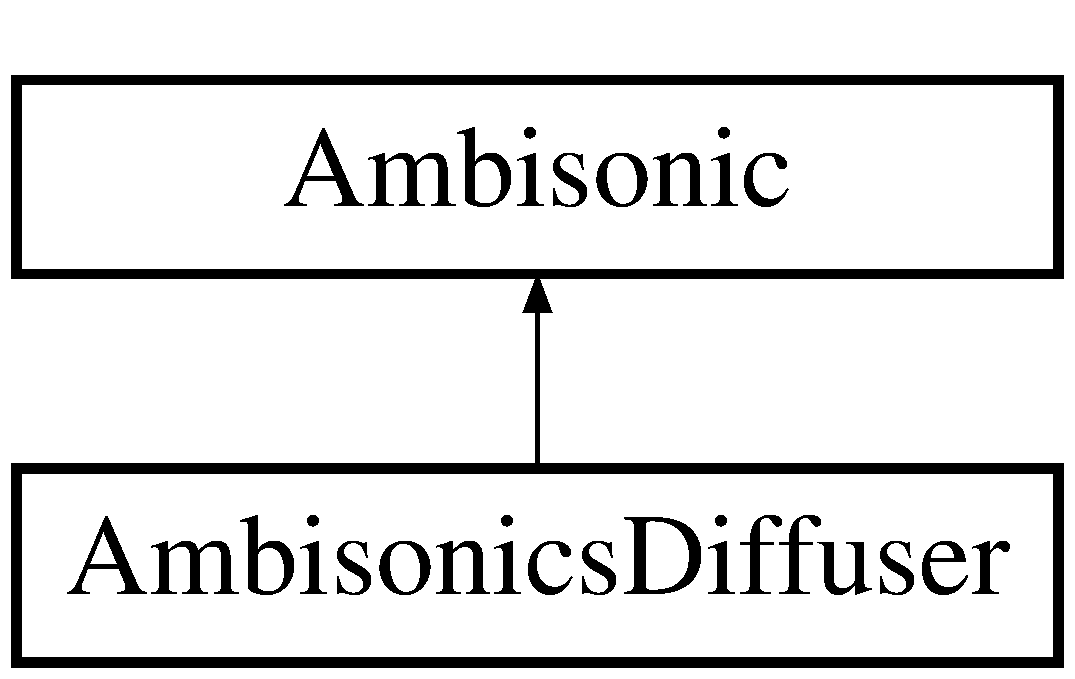
\includegraphics[height=3.000000cm]{class_ambisonics_diffuser}
\end{center}
\end{figure}
\subsection*{Public Member Functions}
\begin{DoxyCompactItemize}
\item 
\hyperlink{class_ambisonics_diffuser_a3cb3d33fc7fc15d85b337860c2a0fc34}{Ambisonics\-Diffuser} (long an\-Order=1, bool a\-Mode=Hoa\-\_\-\-Post\-\_\-\-Encoding, long a\-Vector\-Size=0, long a\-Sampling\-Rate=44100.)
\end{DoxyCompactItemize}


\subsection{Detailed Description}


Definition at line 38 of file Ambisonics\-Diffuser.\-h.



\subsection{Constructor \& Destructor Documentation}
\hypertarget{class_ambisonics_diffuser_a3cb3d33fc7fc15d85b337860c2a0fc34}{\index{Ambisonics\-Diffuser@{Ambisonics\-Diffuser}!Ambisonics\-Diffuser@{Ambisonics\-Diffuser}}
\index{Ambisonics\-Diffuser@{Ambisonics\-Diffuser}!AmbisonicsDiffuser@{Ambisonics\-Diffuser}}
\subsubsection[{Ambisonics\-Diffuser}]{\setlength{\rightskip}{0pt plus 5cm}Ambisonics\-Diffuser\-::\-Ambisonics\-Diffuser (
\begin{DoxyParamCaption}
\item[{long}]{an\-Order = {\ttfamily 1}, }
\item[{bool}]{a\-Mode = {\ttfamily Hoa\-\_\-Post\-\_\-Encoding}, }
\item[{long}]{a\-Vector\-Size = {\ttfamily 0}, }
\item[{long}]{a\-Sampling\-Rate = {\ttfamily 44100.}}
\end{DoxyParamCaption}
)}}\label{class_ambisonics_diffuser_a3cb3d33fc7fc15d85b337860c2a0fc34}
Hoa\-Library \-: A High Order Ambisonics Library Copyright (c) 2012-\/2013 Julien Colafrancesco, Pierre Guillot, Eliott Paris, C\-I\-C\-M, Universite Paris-\/8. All rights reserved.\-re Guillot, C\-I\-C\-M -\/ Université Paris 8 All rights reserved.

Website \-: \href{http://www.mshparisnord.fr/HoaLibrary/}{\tt http\-://www.\-mshparisnord.\-fr/\-Hoa\-Library/} Contacts \-: \href{mailto:cicm.mshparisnord@gmail.com}{\tt cicm.\-mshparisnord@gmail.\-com}

This file is part of H\-O\-A L\-I\-B\-R\-A\-R\-Y.

H\-O\-A L\-I\-B\-R\-A\-R\-Y is free software\-: you can redistribute it and/or modify it under the terms of the G\-N\-U General Public License as published by the Free Software Foundation, either version 3 of the License, or (at your option) any later version.

This program is distributed in the hope that it will be useful, but W\-I\-T\-H\-O\-U\-T A\-N\-Y W\-A\-R\-R\-A\-N\-T\-Y; without even the implied warranty of M\-E\-R\-C\-H\-A\-N\-T\-A\-B\-I\-L\-I\-T\-Y or F\-I\-T\-N\-E\-S\-S F\-O\-R A P\-A\-R\-T\-I\-C\-U\-L\-A\-R P\-U\-R\-P\-O\-S\-E. See the G\-N\-U General Public License for more details.

You should have received a copy of the G\-N\-U General Public License along with this program. If not, see \href{http://www.gnu.org/licenses/}{\tt http\-://www.\-gnu.\-org/licenses/}. 

Definition at line 29 of file Ambisonics\-Diffuser.\-cpp.



The documentation for this class was generated from the following files\-:\begin{DoxyCompactItemize}
\item 
/\-Users/elioton/\-Documents/programmation/\-C\-I\-C\-M/source\-Tree/\-Hoa\-Library/\-Sources/hoa\-Ambisonics/Ambisonics\-Diffuser.\-h\item 
/\-Users/elioton/\-Documents/programmation/\-C\-I\-C\-M/source\-Tree/\-Hoa\-Library/\-Sources/hoa\-Ambisonics/Ambisonics\-Diffuser.\-cpp\end{DoxyCompactItemize}

\hypertarget{class_ambisonics_filter}{\section{Ambisonics\-Filter Class Reference}
\label{class_ambisonics_filter}\index{Ambisonics\-Filter@{Ambisonics\-Filter}}
}


{\ttfamily \#include $<$Ambisonics\-Filter.\-h$>$}

Inheritance diagram for Ambisonics\-Filter\-:\begin{figure}[H]
\begin{center}
\leavevmode
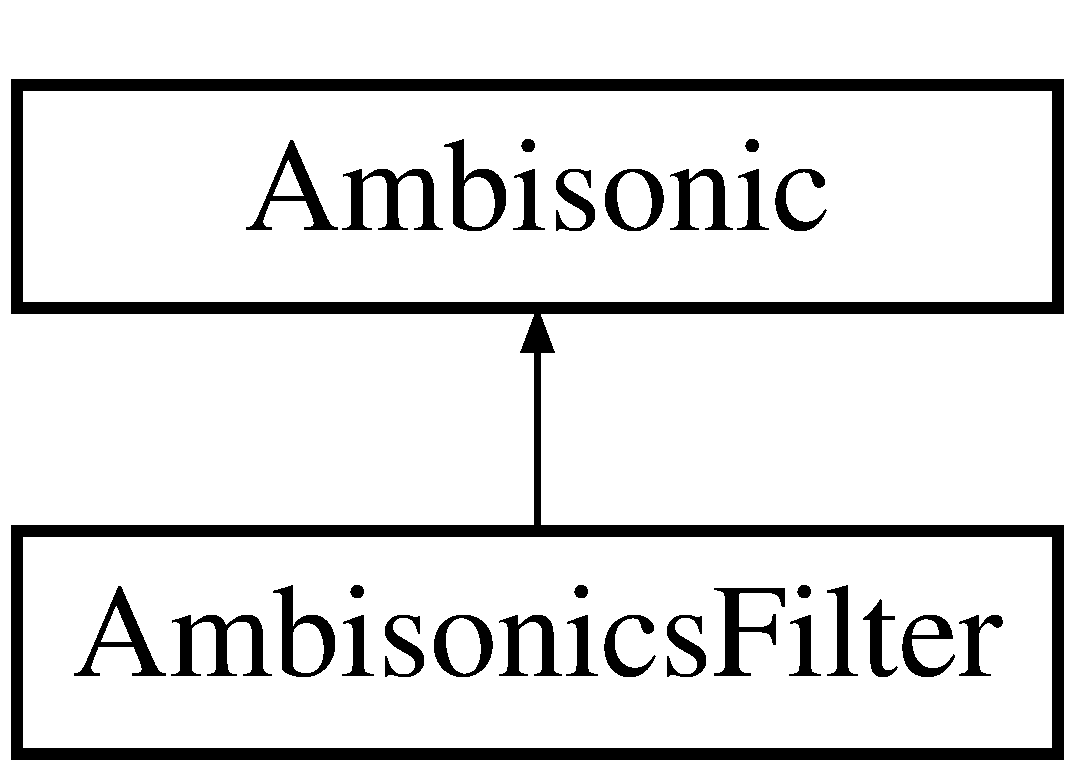
\includegraphics[height=2.000000cm]{class_ambisonics_filter}
\end{center}
\end{figure}
\subsection*{Public Member Functions}
\begin{DoxyCompactItemize}
\item 
\hyperlink{class_ambisonics_filter_aeeafcaad4a5d3081d777c3e8bb03ed0c}{Ambisonics\-Filter} (long an\-Order=1, long a\-Vector\-Size=0, long a\-Sampling\-Rate=44100)
\item 
\hypertarget{class_ambisonics_filter_acdbc7e48c9e6d989c1dc103f386e5a3f}{void {\bfseries set\-Diffusion} (double a\-Diffuse\-Factor)}\label{class_ambisonics_filter_acdbc7e48c9e6d989c1dc103f386e5a3f}

\item 
\hypertarget{class_ambisonics_filter_acfb84d5862c9c9fe837d2786c10d21dd}{double {\bfseries get\-Diffusion} ()}\label{class_ambisonics_filter_acfb84d5862c9c9fe837d2786c10d21dd}

\item 
\hypertarget{class_ambisonics_filter_a223e952d03990b8c54131754a74e018c}{void {\bfseries set\-Frequency\-Band} (long an\-Index, double a\-Frequency)}\label{class_ambisonics_filter_a223e952d03990b8c54131754a74e018c}

\item 
\hypertarget{class_ambisonics_filter_a5e1196b6f8470a264edbe9dcb5072afe}{double {\bfseries get\-Frequency\-Band} (long an\-Index)}\label{class_ambisonics_filter_a5e1196b6f8470a264edbe9dcb5072afe}

\item 
\hypertarget{class_ambisonics_filter_a13b6286ca6514a6601245050f684f66f}{void {\bfseries set\-Vector\-Size} (long a\-Vector\-Size)}\label{class_ambisonics_filter_a13b6286ca6514a6601245050f684f66f}

\item 
\hypertarget{class_ambisonics_filter_ae671de830a2c29e0624de0c433622f5f}{void {\bfseries set\-Sampling\-Rate} (long a\-Sampling\-Rate)}\label{class_ambisonics_filter_ae671de830a2c29e0624de0c433622f5f}

\item 
\hypertarget{class_ambisonics_filter_abef4dd5c6a7a1e35a87191f31e0094c6}{void {\bfseries process} (float $\ast$inputs, float $\ast$outputs)}\label{class_ambisonics_filter_abef4dd5c6a7a1e35a87191f31e0094c6}

\item 
\hypertarget{class_ambisonics_filter_a2357b427c1838b0eb287be4afdab955c}{void {\bfseries process} (double $\ast$inputs, double $\ast$outputs)}\label{class_ambisonics_filter_a2357b427c1838b0eb287be4afdab955c}

\item 
\hypertarget{class_ambisonics_filter_a9b73f86d05ba949a47faeddf89800e9c}{void {\bfseries process} (float $\ast$$\ast$inputs, float $\ast$$\ast$outputs)}\label{class_ambisonics_filter_a9b73f86d05ba949a47faeddf89800e9c}

\item 
\hypertarget{class_ambisonics_filter_a1a9abff888e189929ba9ea345adf66ba}{void {\bfseries process} (double $\ast$$\ast$inputs, double $\ast$$\ast$outputs)}\label{class_ambisonics_filter_a1a9abff888e189929ba9ea345adf66ba}

\end{DoxyCompactItemize}
\subsection*{Additional Inherited Members}


\subsection{Detailed Description}
\hyperlink{interface_hoa_library}{Hoa\-Library} \-: A High Order Ambisonics Library Copyright (c) 2012-\/2013 Julien Colafrancesco, Pierre Guillot, Eliott Paris, C\-I\-C\-M, Universite Paris-\/8. All rights reserved.\-re Guillot, C\-I\-C\-M -\/ Université Paris 8 All rights reserved.

Website \-: \href{http://www.mshparisnord.fr/HoaLibrary/}{\tt http\-://www.\-mshparisnord.\-fr/\-Hoa\-Library/} Contacts \-: \href{mailto:cicm.mshparisnord@gmail.com}{\tt cicm.\-mshparisnord@gmail.\-com}

This file is part of H\-O\-A L\-I\-B\-R\-A\-R\-Y.

H\-O\-A L\-I\-B\-R\-A\-R\-Y is free software\-: you can redistribute it and/or modify it under the terms of the G\-N\-U General Public License as published by the Free Software Foundation, either version 3 of the License, or (at your option) any later version.

This program is distributed in the hope that it will be useful, but W\-I\-T\-H\-O\-U\-T A\-N\-Y W\-A\-R\-R\-A\-N\-T\-Y; without even the implied warranty of M\-E\-R\-C\-H\-A\-N\-T\-A\-B\-I\-L\-I\-T\-Y or F\-I\-T\-N\-E\-S\-S F\-O\-R A P\-A\-R\-T\-I\-C\-U\-L\-A\-R P\-U\-R\-P\-O\-S\-E. See the G\-N\-U General Public License for more details.

You should have received a copy of the G\-N\-U General Public License along with this program. If not, see \href{http://www.gnu.org/licenses/}{\tt http\-://www.\-gnu.\-org/licenses/}. 

\subsection{Constructor \& Destructor Documentation}
\hypertarget{class_ambisonics_filter_aeeafcaad4a5d3081d777c3e8bb03ed0c}{\index{Ambisonics\-Filter@{Ambisonics\-Filter}!Ambisonics\-Filter@{Ambisonics\-Filter}}
\index{Ambisonics\-Filter@{Ambisonics\-Filter}!AmbisonicsFilter@{Ambisonics\-Filter}}
\subsubsection[{Ambisonics\-Filter}]{\setlength{\rightskip}{0pt plus 5cm}Ambisonics\-Filter\-::\-Ambisonics\-Filter (
\begin{DoxyParamCaption}
\item[{long}]{an\-Order = {\ttfamily 1}, }
\item[{long}]{a\-Vector\-Size = {\ttfamily 0}, }
\item[{long}]{a\-Sampling\-Rate = {\ttfamily 44100}}
\end{DoxyParamCaption}
)}}\label{class_ambisonics_filter_aeeafcaad4a5d3081d777c3e8bb03ed0c}
\hyperlink{interface_hoa_library}{Hoa\-Library} \-: A High Order Ambisonics Library Copyright (c) 2012-\/2013 Julien Colafrancesco, Pierre Guillot, Eliott Paris, C\-I\-C\-M, Universite Paris-\/8. All rights reserved.\-re Guillot, C\-I\-C\-M -\/ Université Paris 8 All rights reserved.

Website \-: \href{http://www.mshparisnord.fr/HoaLibrary/}{\tt http\-://www.\-mshparisnord.\-fr/\-Hoa\-Library/} Contacts \-: \href{mailto:cicm.mshparisnord@gmail.com}{\tt cicm.\-mshparisnord@gmail.\-com}

This file is part of H\-O\-A L\-I\-B\-R\-A\-R\-Y.

H\-O\-A L\-I\-B\-R\-A\-R\-Y is free software\-: you can redistribute it and/or modify it under the terms of the G\-N\-U General Public License as published by the Free Software Foundation, either version 3 of the License, or (at your option) any later version.

This program is distributed in the hope that it will be useful, but W\-I\-T\-H\-O\-U\-T A\-N\-Y W\-A\-R\-R\-A\-N\-T\-Y; without even the implied warranty of M\-E\-R\-C\-H\-A\-N\-T\-A\-B\-I\-L\-I\-T\-Y or F\-I\-T\-N\-E\-S\-S F\-O\-R A P\-A\-R\-T\-I\-C\-U\-L\-A\-R P\-U\-R\-P\-O\-S\-E. See the G\-N\-U General Public License for more details.

You should have received a copy of the G\-N\-U General Public License along with this program. If not, see \href{http://www.gnu.org/licenses/}{\tt http\-://www.\-gnu.\-org/licenses/}. 

The documentation for this class was generated from the following files\-:\begin{DoxyCompactItemize}
\item 
/\-Users/\-Pierre/\-Source\-Tree/\-Hoa\-Library/\-Sources/hoa\-Filter/Ambisonics\-Filter.\-h\item 
/\-Users/\-Pierre/\-Source\-Tree/\-Hoa\-Library/\-Sources/hoa\-Filter/Ambisonics\-Filter.\-cpp\end{DoxyCompactItemize}

\hypertarget{class_ambisonics_freeverb}{\section{Ambisonics\-Freeverb Class Reference}
\label{class_ambisonics_freeverb}\index{Ambisonics\-Freeverb@{Ambisonics\-Freeverb}}
}


{\ttfamily \#include $<$Ambisonics\-Freeverb.\-h$>$}

Inheritance diagram for Ambisonics\-Freeverb\-:\begin{figure}[H]
\begin{center}
\leavevmode
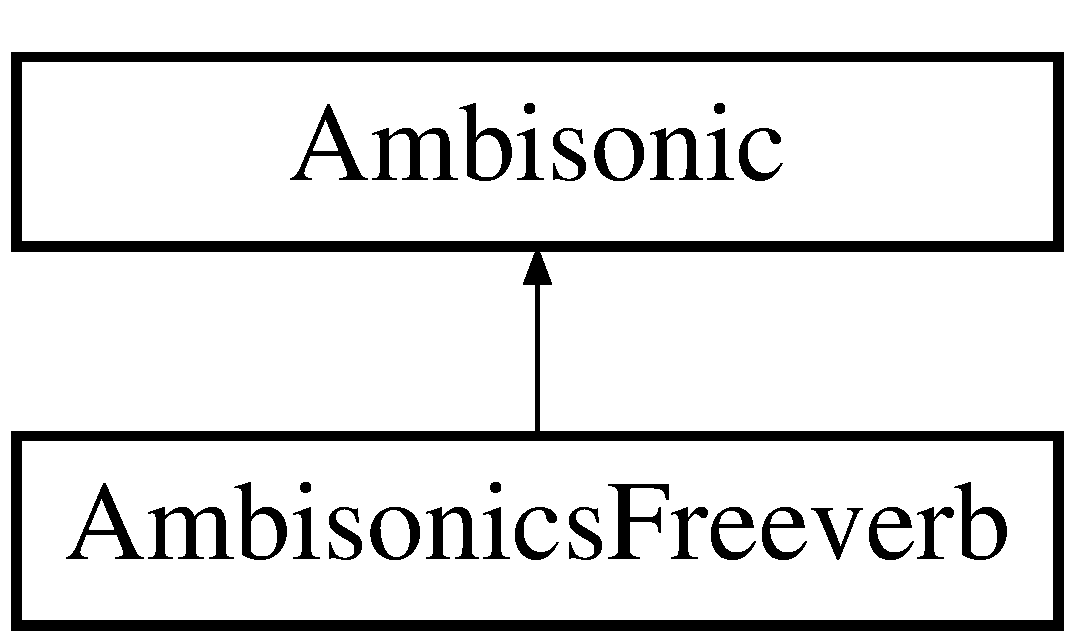
\includegraphics[height=2.000000cm]{class_ambisonics_freeverb}
\end{center}
\end{figure}
\subsection*{Public Member Functions}
\begin{DoxyCompactItemize}
\item 
\hyperlink{class_ambisonics_freeverb_a837e51d85f2a237e7957b6534f3bde1c}{Ambisonics\-Freeverb} (long an\-Order=1, long a\-Vector\-Size=0, double a\-Sampling\-Rate=44100.)
\end{DoxyCompactItemize}


\subsection{Detailed Description}
\hyperlink{interface_hoa_library}{Hoa\-Library} \-: A High Order Ambisonics Library Copyright (c) 2012-\/2013 Julien Colafrancesco, Pierre Guillot, Eliott Paris, C\-I\-C\-M, Universite Paris-\/8. All rights reserved.

Website \-: \href{http://www.mshparisnord.fr/hoalibrary/}{\tt http\-://www.\-mshparisnord.\-fr/hoalibrary/} Contacts \-: \href{mailto:cicm.mshparisnord@gmail.com}{\tt cicm.\-mshparisnord@gmail.\-com}

Redistribution and use in source and binary forms, with or without modification, are permitted provided that the following conditions are met\-:


\begin{DoxyItemize}
\item Redistributions may not be sold, nor may they be used in a commercial product or activity.
\item Redistributions of source code must retain the above copyright notice, this list of conditions and the following disclaimer.
\item Redistributions in binary form must reproduce the above copyright notice, this list of conditions and the following disclaimer in the documentation and/or other materials provided with the distribution.
\item Neither the name of the C\-I\-C\-M nor the names of its contributors may be used to endorse or promote products derived from this software without specific prior written permission.
\end{DoxyItemize}

T\-H\-I\-S S\-O\-F\-T\-W\-A\-R\-E I\-S P\-R\-O\-V\-I\-D\-E\-D B\-Y T\-H\-E C\-O\-P\-Y\-R\-I\-G\-H\-T H\-O\-L\-D\-E\-R\-S A\-N\-D C\-O\-N\-T\-R\-I\-B\-U\-T\-O\-R\-S \char`\"{}\-A\-S I\-S\char`\"{} A\-N\-D A\-N\-Y E\-X\-P\-R\-E\-S\-S O\-R I\-M\-P\-L\-I\-E\-D W\-A\-R\-R\-A\-N\-T\-I\-E\-S, I\-N\-C\-L\-U\-D\-I\-N\-G, B\-U\-T N\-O\-T L\-I\-M\-I\-T\-E\-D T\-O, T\-H\-E I\-M\-P\-L\-I\-E\-D W\-A\-R\-R\-A\-N\-T\-I\-E\-S O\-F M\-E\-R\-C\-H\-A\-N\-T\-A\-B\-I\-L\-I\-T\-Y A\-N\-D F\-I\-T\-N\-E\-S\-S F\-O\-R A P\-A\-R\-T\-I\-C\-U\-L\-A\-R P\-U\-R\-P\-O\-S\-E A\-R\-E D\-I\-S\-C\-L\-A\-I\-M\-E\-D. I\-N N\-O E\-V\-E\-N\-T S\-H\-A\-L\-L T\-H\-E C\-O\-P\-Y\-R\-I\-G\-H\-T H\-O\-L\-D\-E\-R O\-R C\-O\-N\-T\-R\-I\-B\-U\-T\-O\-R\-S B\-E L\-I\-A\-B\-L\-E F\-O\-R A\-N\-Y D\-I\-R\-E\-C\-T, I\-N\-D\-I\-R\-E\-C\-T, I\-N\-C\-I\-D\-E\-N\-T\-A\-L, S\-P\-E\-C\-I\-A\-L, E\-X\-E\-M\-P\-L\-A\-R\-Y, O\-R C\-O\-N\-S\-E\-Q\-U\-E\-N\-T\-I\-A\-L D\-A\-M\-A\-G\-E\-S (I\-N\-C\-L\-U\-D\-I\-N\-G, B\-U\-T N\-O\-T L\-I\-M\-I\-T\-E\-D T\-O, P\-R\-O\-C\-U\-R\-E\-M\-E\-N\-T O\-F S\-U\-B\-S\-T\-I\-T\-U\-T\-E G\-O\-O\-D\-S O\-R S\-E\-R\-V\-I\-C\-E\-S; L\-O\-S\-S O\-F U\-S\-E, D\-A\-T\-A, O\-R P\-R\-O\-F\-I\-T\-S; O\-R B\-U\-S\-I\-N\-E\-S\-S I\-N\-T\-E\-R\-R\-U\-P\-T\-I\-O\-N) H\-O\-W\-E\-V\-E\-R C\-A\-U\-S\-E\-D A\-N\-D O\-N A\-N\-Y T\-H\-E\-O\-R\-Y O\-F L\-I\-A\-B\-I\-L\-I\-T\-Y, W\-H\-E\-T\-H\-E\-R I\-N C\-O\-N\-T\-R\-A\-C\-T, S\-T\-R\-I\-C\-T L\-I\-A\-B\-I\-L\-I\-T\-Y, O\-R T\-O\-R\-T (I\-N\-C\-L\-U\-D\-I\-N\-G N\-E\-G\-L\-I\-G\-E\-N\-C\-E O\-R O\-T\-H\-E\-R\-W\-I\-S\-E) A\-R\-I\-S\-I\-N\-G I\-N A\-N\-Y W\-A\-Y O\-U\-T O\-F T\-H\-E U\-S\-E O\-F T\-H\-I\-S S\-O\-F\-T\-W\-A\-R\-E, E\-V\-E\-N I\-F A\-D\-V\-I\-S\-E\-D O\-F T\-H\-E P\-O\-S\-S\-I\-B\-I\-L\-I\-T\-Y O\-F S\-U\-C\-H D\-A\-M\-A\-G\-E. 

Definition at line 31 of file Ambisonics\-Freeverb.\-h.



\subsection{Constructor \& Destructor Documentation}
\hypertarget{class_ambisonics_freeverb_a837e51d85f2a237e7957b6534f3bde1c}{\index{Ambisonics\-Freeverb@{Ambisonics\-Freeverb}!Ambisonics\-Freeverb@{Ambisonics\-Freeverb}}
\index{Ambisonics\-Freeverb@{Ambisonics\-Freeverb}!AmbisonicsFreeverb@{Ambisonics\-Freeverb}}
\subsubsection[{Ambisonics\-Freeverb}]{\setlength{\rightskip}{0pt plus 5cm}Ambisonics\-Freeverb\-::\-Ambisonics\-Freeverb (
\begin{DoxyParamCaption}
\item[{long}]{an\-Order = {\ttfamily 1}, }
\item[{long}]{a\-Vector\-Size = {\ttfamily 0}, }
\item[{double}]{a\-Sampling\-Rate = {\ttfamily 44100.}}
\end{DoxyParamCaption}
)}}\label{class_ambisonics_freeverb_a837e51d85f2a237e7957b6534f3bde1c}
\hyperlink{interface_hoa_library}{Hoa\-Library} \-: A High Order Ambisonics Library Copyright (c) 2012-\/2013 Julien Colafrancesco, Pierre Guillot, Eliott Paris, C\-I\-C\-M, Universite Paris-\/8. All rights reserved.

Website \-: \href{http://www.mshparisnord.fr/hoalibrary/}{\tt http\-://www.\-mshparisnord.\-fr/hoalibrary/} Contacts \-: \href{mailto:cicm.mshparisnord@gmail.com}{\tt cicm.\-mshparisnord@gmail.\-com}

Redistribution and use in source and binary forms, with or without modification, are permitted provided that the following conditions are met\-:


\begin{DoxyItemize}
\item Redistributions may not be sold, nor may they be used in a commercial product or activity.
\item Redistributions of source code must retain the above copyright notice, this list of conditions and the following disclaimer.
\item Redistributions in binary form must reproduce the above copyright notice, this list of conditions and the following disclaimer in the documentation and/or other materials provided with the distribution.
\item Neither the name of the C\-I\-C\-M nor the names of its contributors may be used to endorse or promote products derived from this software without specific prior written permission.
\end{DoxyItemize}

T\-H\-I\-S S\-O\-F\-T\-W\-A\-R\-E I\-S P\-R\-O\-V\-I\-D\-E\-D B\-Y T\-H\-E C\-O\-P\-Y\-R\-I\-G\-H\-T H\-O\-L\-D\-E\-R\-S A\-N\-D C\-O\-N\-T\-R\-I\-B\-U\-T\-O\-R\-S \char`\"{}\-A\-S I\-S\char`\"{} A\-N\-D A\-N\-Y E\-X\-P\-R\-E\-S\-S O\-R I\-M\-P\-L\-I\-E\-D W\-A\-R\-R\-A\-N\-T\-I\-E\-S, I\-N\-C\-L\-U\-D\-I\-N\-G, B\-U\-T N\-O\-T L\-I\-M\-I\-T\-E\-D T\-O, T\-H\-E I\-M\-P\-L\-I\-E\-D W\-A\-R\-R\-A\-N\-T\-I\-E\-S O\-F M\-E\-R\-C\-H\-A\-N\-T\-A\-B\-I\-L\-I\-T\-Y A\-N\-D F\-I\-T\-N\-E\-S\-S F\-O\-R A P\-A\-R\-T\-I\-C\-U\-L\-A\-R P\-U\-R\-P\-O\-S\-E A\-R\-E D\-I\-S\-C\-L\-A\-I\-M\-E\-D. I\-N N\-O E\-V\-E\-N\-T S\-H\-A\-L\-L T\-H\-E C\-O\-P\-Y\-R\-I\-G\-H\-T H\-O\-L\-D\-E\-R O\-R C\-O\-N\-T\-R\-I\-B\-U\-T\-O\-R\-S B\-E L\-I\-A\-B\-L\-E F\-O\-R A\-N\-Y D\-I\-R\-E\-C\-T, I\-N\-D\-I\-R\-E\-C\-T, I\-N\-C\-I\-D\-E\-N\-T\-A\-L, S\-P\-E\-C\-I\-A\-L, E\-X\-E\-M\-P\-L\-A\-R\-Y, O\-R C\-O\-N\-S\-E\-Q\-U\-E\-N\-T\-I\-A\-L D\-A\-M\-A\-G\-E\-S (I\-N\-C\-L\-U\-D\-I\-N\-G, B\-U\-T N\-O\-T L\-I\-M\-I\-T\-E\-D T\-O, P\-R\-O\-C\-U\-R\-E\-M\-E\-N\-T O\-F S\-U\-B\-S\-T\-I\-T\-U\-T\-E G\-O\-O\-D\-S O\-R S\-E\-R\-V\-I\-C\-E\-S; L\-O\-S\-S O\-F U\-S\-E, D\-A\-T\-A, O\-R P\-R\-O\-F\-I\-T\-S; O\-R B\-U\-S\-I\-N\-E\-S\-S I\-N\-T\-E\-R\-R\-U\-P\-T\-I\-O\-N) H\-O\-W\-E\-V\-E\-R C\-A\-U\-S\-E\-D A\-N\-D O\-N A\-N\-Y T\-H\-E\-O\-R\-Y O\-F L\-I\-A\-B\-I\-L\-I\-T\-Y, W\-H\-E\-T\-H\-E\-R I\-N C\-O\-N\-T\-R\-A\-C\-T, S\-T\-R\-I\-C\-T L\-I\-A\-B\-I\-L\-I\-T\-Y, O\-R T\-O\-R\-T (I\-N\-C\-L\-U\-D\-I\-N\-G N\-E\-G\-L\-I\-G\-E\-N\-C\-E O\-R O\-T\-H\-E\-R\-W\-I\-S\-E) A\-R\-I\-S\-I\-N\-G I\-N A\-N\-Y W\-A\-Y O\-U\-T O\-F T\-H\-E U\-S\-E O\-F T\-H\-I\-S S\-O\-F\-T\-W\-A\-R\-E, E\-V\-E\-N I\-F A\-D\-V\-I\-S\-E\-D O\-F T\-H\-E P\-O\-S\-S\-I\-B\-I\-L\-I\-T\-Y O\-F S\-U\-C\-H D\-A\-M\-A\-G\-E. 

Definition at line 28 of file Ambisonics\-Freeverb.\-cpp.



The documentation for this class was generated from the following files\-:\begin{DoxyCompactItemize}
\item 
/\-Users/elioton/\-Documents/programmation/\-C\-I\-C\-M/source\-Tree/\-Hoa\-Library/\-Sources/hoa\-Freeverb/Ambisonics\-Freeverb.\-h\item 
/\-Users/elioton/\-Documents/programmation/\-C\-I\-C\-M/source\-Tree/\-Hoa\-Library/\-Sources/hoa\-Freeverb/Ambisonics\-Freeverb.\-cpp\end{DoxyCompactItemize}

\hypertarget{class_ambisonics_grain}{\section{Ambisonics\-Grain Class Reference}
\label{class_ambisonics_grain}\index{Ambisonics\-Grain@{Ambisonics\-Grain}}
}


{\ttfamily \#include $<$Ambisonics\-Grain.\-h$>$}

Inheritance diagram for Ambisonics\-Grain\-:\begin{figure}[H]
\begin{center}
\leavevmode
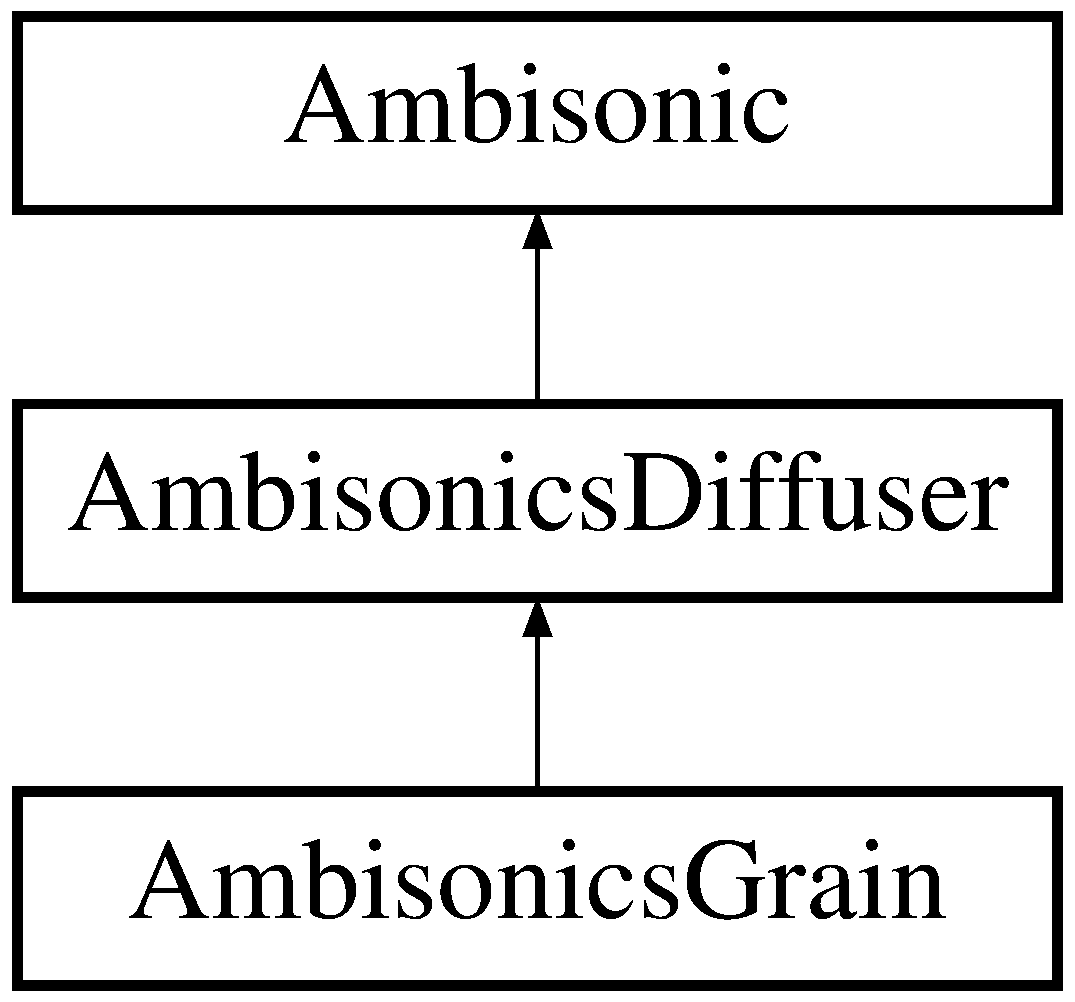
\includegraphics[height=3.000000cm]{class_ambisonics_grain}
\end{center}
\end{figure}
\subsection*{Public Member Functions}
\begin{DoxyCompactItemize}
\item 
\hyperlink{class_ambisonics_grain_a5e83b470e8597a5dd7b11860ef6fd456}{Ambisonics\-Grain} (long an\-Order=1, bool a\-Mode=Hoa\-\_\-\-Post\-\_\-\-Encoding, double a\-Maximum\-Delay\-In\-Ms=5000., long a\-Vector\-Size=0, long a\-Sampling\-Rate=44100)
\end{DoxyCompactItemize}


\subsection{Detailed Description}
Hoa\-Library \-: A High Order Ambisonics Library Copyright (c) 2012-\/2013 Julien Colafrancesco, Pierre Guillot, Eliott Paris, C\-I\-C\-M, Universite Paris-\/8. All rights reserved.

Website \-: \href{http://www.mshparisnord.fr/hoalibrary/}{\tt http\-://www.\-mshparisnord.\-fr/hoalibrary/} Contacts \-: \href{mailto:cicm.mshparisnord@gmail.com}{\tt cicm.\-mshparisnord@gmail.\-com}

Redistribution and use in source and binary forms, with or without modification, are permitted provided that the following conditions are met\-:


\begin{DoxyItemize}
\item Redistributions may not be sold, nor may they be used in a commercial product or activity.
\item Redistributions of source code must retain the above copyright notice, this list of conditions and the following disclaimer.
\item Redistributions in binary form must reproduce the above copyright notice, this list of conditions and the following disclaimer in the documentation and/or other materials provided with the distribution.
\item Neither the name of the C\-I\-C\-M nor the names of its contributors may be used to endorse or promote products derived from this software without specific prior written permission.
\end{DoxyItemize}

T\-H\-I\-S S\-O\-F\-T\-W\-A\-R\-E I\-S P\-R\-O\-V\-I\-D\-E\-D B\-Y T\-H\-E C\-O\-P\-Y\-R\-I\-G\-H\-T H\-O\-L\-D\-E\-R\-S A\-N\-D C\-O\-N\-T\-R\-I\-B\-U\-T\-O\-R\-S \char`\"{}\-A\-S I\-S\char`\"{} A\-N\-D A\-N\-Y E\-X\-P\-R\-E\-S\-S O\-R I\-M\-P\-L\-I\-E\-D W\-A\-R\-R\-A\-N\-T\-I\-E\-S, I\-N\-C\-L\-U\-D\-I\-N\-G, B\-U\-T N\-O\-T L\-I\-M\-I\-T\-E\-D T\-O, T\-H\-E I\-M\-P\-L\-I\-E\-D W\-A\-R\-R\-A\-N\-T\-I\-E\-S O\-F M\-E\-R\-C\-H\-A\-N\-T\-A\-B\-I\-L\-I\-T\-Y A\-N\-D F\-I\-T\-N\-E\-S\-S F\-O\-R A P\-A\-R\-T\-I\-C\-U\-L\-A\-R P\-U\-R\-P\-O\-S\-E A\-R\-E D\-I\-S\-C\-L\-A\-I\-M\-E\-D. I\-N N\-O E\-V\-E\-N\-T S\-H\-A\-L\-L T\-H\-E C\-O\-P\-Y\-R\-I\-G\-H\-T H\-O\-L\-D\-E\-R O\-R C\-O\-N\-T\-R\-I\-B\-U\-T\-O\-R\-S B\-E L\-I\-A\-B\-L\-E F\-O\-R A\-N\-Y D\-I\-R\-E\-C\-T, I\-N\-D\-I\-R\-E\-C\-T, I\-N\-C\-I\-D\-E\-N\-T\-A\-L, S\-P\-E\-C\-I\-A\-L, E\-X\-E\-M\-P\-L\-A\-R\-Y, O\-R C\-O\-N\-S\-E\-Q\-U\-E\-N\-T\-I\-A\-L D\-A\-M\-A\-G\-E\-S (I\-N\-C\-L\-U\-D\-I\-N\-G, B\-U\-T N\-O\-T L\-I\-M\-I\-T\-E\-D T\-O, P\-R\-O\-C\-U\-R\-E\-M\-E\-N\-T O\-F S\-U\-B\-S\-T\-I\-T\-U\-T\-E G\-O\-O\-D\-S O\-R S\-E\-R\-V\-I\-C\-E\-S; L\-O\-S\-S O\-F U\-S\-E, D\-A\-T\-A, O\-R P\-R\-O\-F\-I\-T\-S; O\-R B\-U\-S\-I\-N\-E\-S\-S I\-N\-T\-E\-R\-R\-U\-P\-T\-I\-O\-N) H\-O\-W\-E\-V\-E\-R C\-A\-U\-S\-E\-D A\-N\-D O\-N A\-N\-Y T\-H\-E\-O\-R\-Y O\-F L\-I\-A\-B\-I\-L\-I\-T\-Y, W\-H\-E\-T\-H\-E\-R I\-N C\-O\-N\-T\-R\-A\-C\-T, S\-T\-R\-I\-C\-T L\-I\-A\-B\-I\-L\-I\-T\-Y, O\-R T\-O\-R\-T (I\-N\-C\-L\-U\-D\-I\-N\-G N\-E\-G\-L\-I\-G\-E\-N\-C\-E O\-R O\-T\-H\-E\-R\-W\-I\-S\-E) A\-R\-I\-S\-I\-N\-G I\-N A\-N\-Y W\-A\-Y O\-U\-T O\-F T\-H\-E U\-S\-E O\-F T\-H\-I\-S S\-O\-F\-T\-W\-A\-R\-E, E\-V\-E\-N I\-F A\-D\-V\-I\-S\-E\-D O\-F T\-H\-E P\-O\-S\-S\-I\-B\-I\-L\-I\-T\-Y O\-F S\-U\-C\-H D\-A\-M\-A\-G\-E. 

Definition at line 31 of file Ambisonics\-Grain.\-h.



\subsection{Constructor \& Destructor Documentation}
\hypertarget{class_ambisonics_grain_a5e83b470e8597a5dd7b11860ef6fd456}{\index{Ambisonics\-Grain@{Ambisonics\-Grain}!Ambisonics\-Grain@{Ambisonics\-Grain}}
\index{Ambisonics\-Grain@{Ambisonics\-Grain}!AmbisonicsGrain@{Ambisonics\-Grain}}
\subsubsection[{Ambisonics\-Grain}]{\setlength{\rightskip}{0pt plus 5cm}Ambisonics\-Grain\-::\-Ambisonics\-Grain (
\begin{DoxyParamCaption}
\item[{long}]{an\-Order = {\ttfamily 1}, }
\item[{bool}]{a\-Mode = {\ttfamily Hoa\-\_\-Post\-\_\-Encoding}, }
\item[{double}]{a\-Maximum\-Delay\-In\-Ms = {\ttfamily 5000.}, }
\item[{long}]{a\-Vector\-Size = {\ttfamily 0}, }
\item[{long}]{a\-Sampling\-Rate = {\ttfamily 44100}}
\end{DoxyParamCaption}
)}}\label{class_ambisonics_grain_a5e83b470e8597a5dd7b11860ef6fd456}
Hoa\-Library \-: A High Order Ambisonics Library Copyright (c) 2012-\/2013 Julien Colafrancesco, Pierre Guillot, Eliott Paris, C\-I\-C\-M, Universite Paris-\/8. All rights reserved.

Website \-: \href{http://www.mshparisnord.fr/hoalibrary/}{\tt http\-://www.\-mshparisnord.\-fr/hoalibrary/} Contacts \-: \href{mailto:cicm.mshparisnord@gmail.com}{\tt cicm.\-mshparisnord@gmail.\-com}

Redistribution and use in source and binary forms, with or without modification, are permitted provided that the following conditions are met\-:


\begin{DoxyItemize}
\item Redistributions may not be sold, nor may they be used in a commercial product or activity.
\item Redistributions of source code must retain the above copyright notice, this list of conditions and the following disclaimer.
\item Redistributions in binary form must reproduce the above copyright notice, this list of conditions and the following disclaimer in the documentation and/or other materials provided with the distribution.
\item Neither the name of the C\-I\-C\-M nor the names of its contributors may be used to endorse or promote products derived from this software without specific prior written permission.
\end{DoxyItemize}

T\-H\-I\-S S\-O\-F\-T\-W\-A\-R\-E I\-S P\-R\-O\-V\-I\-D\-E\-D B\-Y T\-H\-E C\-O\-P\-Y\-R\-I\-G\-H\-T H\-O\-L\-D\-E\-R\-S A\-N\-D C\-O\-N\-T\-R\-I\-B\-U\-T\-O\-R\-S \char`\"{}\-A\-S I\-S\char`\"{} A\-N\-D A\-N\-Y E\-X\-P\-R\-E\-S\-S O\-R I\-M\-P\-L\-I\-E\-D W\-A\-R\-R\-A\-N\-T\-I\-E\-S, I\-N\-C\-L\-U\-D\-I\-N\-G, B\-U\-T N\-O\-T L\-I\-M\-I\-T\-E\-D T\-O, T\-H\-E I\-M\-P\-L\-I\-E\-D W\-A\-R\-R\-A\-N\-T\-I\-E\-S O\-F M\-E\-R\-C\-H\-A\-N\-T\-A\-B\-I\-L\-I\-T\-Y A\-N\-D F\-I\-T\-N\-E\-S\-S F\-O\-R A P\-A\-R\-T\-I\-C\-U\-L\-A\-R P\-U\-R\-P\-O\-S\-E A\-R\-E D\-I\-S\-C\-L\-A\-I\-M\-E\-D. I\-N N\-O E\-V\-E\-N\-T S\-H\-A\-L\-L T\-H\-E C\-O\-P\-Y\-R\-I\-G\-H\-T H\-O\-L\-D\-E\-R O\-R C\-O\-N\-T\-R\-I\-B\-U\-T\-O\-R\-S B\-E L\-I\-A\-B\-L\-E F\-O\-R A\-N\-Y D\-I\-R\-E\-C\-T, I\-N\-D\-I\-R\-E\-C\-T, I\-N\-C\-I\-D\-E\-N\-T\-A\-L, S\-P\-E\-C\-I\-A\-L, E\-X\-E\-M\-P\-L\-A\-R\-Y, O\-R C\-O\-N\-S\-E\-Q\-U\-E\-N\-T\-I\-A\-L D\-A\-M\-A\-G\-E\-S (I\-N\-C\-L\-U\-D\-I\-N\-G, B\-U\-T N\-O\-T L\-I\-M\-I\-T\-E\-D T\-O, P\-R\-O\-C\-U\-R\-E\-M\-E\-N\-T O\-F S\-U\-B\-S\-T\-I\-T\-U\-T\-E G\-O\-O\-D\-S O\-R S\-E\-R\-V\-I\-C\-E\-S; L\-O\-S\-S O\-F U\-S\-E, D\-A\-T\-A, O\-R P\-R\-O\-F\-I\-T\-S; O\-R B\-U\-S\-I\-N\-E\-S\-S I\-N\-T\-E\-R\-R\-U\-P\-T\-I\-O\-N) H\-O\-W\-E\-V\-E\-R C\-A\-U\-S\-E\-D A\-N\-D O\-N A\-N\-Y T\-H\-E\-O\-R\-Y O\-F L\-I\-A\-B\-I\-L\-I\-T\-Y, W\-H\-E\-T\-H\-E\-R I\-N C\-O\-N\-T\-R\-A\-C\-T, S\-T\-R\-I\-C\-T L\-I\-A\-B\-I\-L\-I\-T\-Y, O\-R T\-O\-R\-T (I\-N\-C\-L\-U\-D\-I\-N\-G N\-E\-G\-L\-I\-G\-E\-N\-C\-E O\-R O\-T\-H\-E\-R\-W\-I\-S\-E) A\-R\-I\-S\-I\-N\-G I\-N A\-N\-Y W\-A\-Y O\-U\-T O\-F T\-H\-E U\-S\-E O\-F T\-H\-I\-S S\-O\-F\-T\-W\-A\-R\-E, E\-V\-E\-N I\-F A\-D\-V\-I\-S\-E\-D O\-F T\-H\-E P\-O\-S\-S\-I\-B\-I\-L\-I\-T\-Y O\-F S\-U\-C\-H D\-A\-M\-A\-G\-E. 

Definition at line 28 of file Ambisonics\-Grain.\-cpp.



The documentation for this class was generated from the following files\-:\begin{DoxyCompactItemize}
\item 
/\-Users/\-Pierre/\-Source\-Tree/\-Hoa\-Library/\-Sources/hoa\-Grain/Ambisonics\-Grain.\-h\item 
/\-Users/\-Pierre/\-Source\-Tree/\-Hoa\-Library/\-Sources/hoa\-Grain/Ambisonics\-Grain.\-cpp\end{DoxyCompactItemize}

\hypertarget{class_ambisonics_meter}{\section{Ambisonics\-Meter Class Reference}
\label{class_ambisonics_meter}\index{Ambisonics\-Meter@{Ambisonics\-Meter}}
}


{\ttfamily \#include $<$Ambisonics\-Meter.\-h$>$}

Inheritance diagram for Ambisonics\-Meter\-:\begin{figure}[H]
\begin{center}
\leavevmode
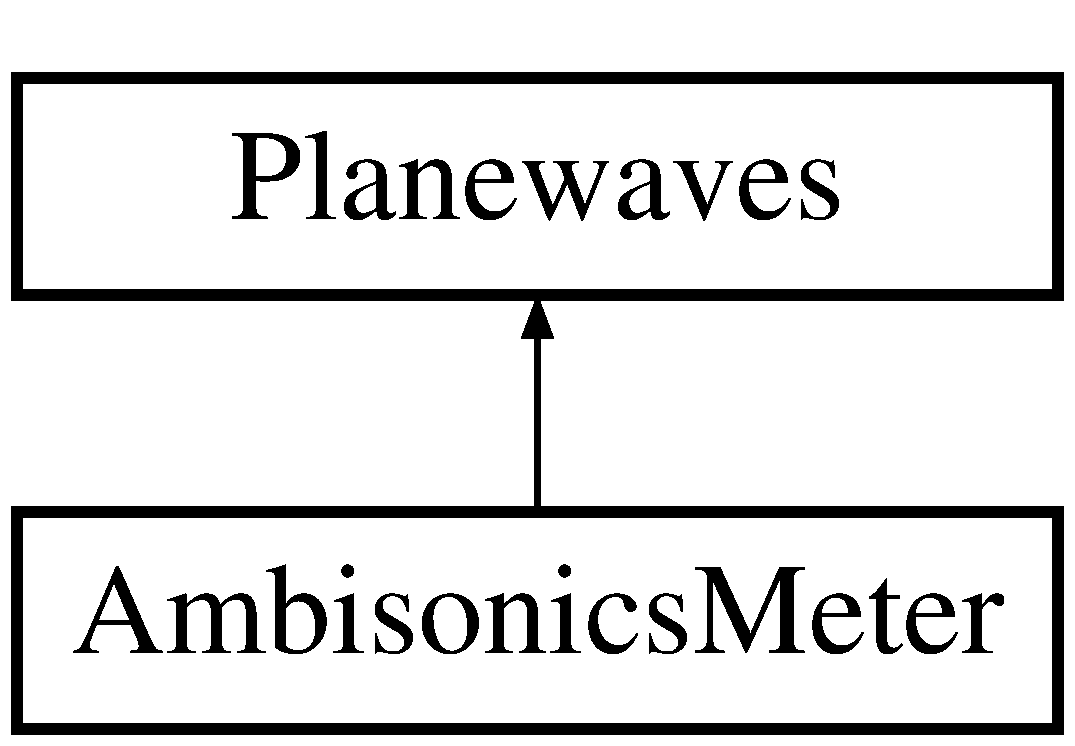
\includegraphics[height=2.000000cm]{class_ambisonics_meter}
\end{center}
\end{figure}
\subsection*{Public Member Functions}
\begin{DoxyCompactItemize}
\item 
\hyperlink{class_ambisonics_meter_ab6652775a732fc5d190101e5673c6758}{Ambisonics\-Meter} (long a\-Number\-Of\-Channel=1, long a\-Vector\-Size=0, double a\-Sampling\-Rate=44100.)
\item 
\hypertarget{class_ambisonics_meter_a67dcdc08682898d4460cf8e04f53a201}{void {\bfseries set\-Number\-Of\-Loudspeakers} (long a\-Number\-Of\-Channels)}\label{class_ambisonics_meter_a67dcdc08682898d4460cf8e04f53a201}

\item 
\hypertarget{class_ambisonics_meter_a14720821cf28453bc1609a234121c040}{void {\bfseries set\-Vector\-Size} (long a\-Vector\-Size)}\label{class_ambisonics_meter_a14720821cf28453bc1609a234121c040}

\item 
\hypertarget{class_ambisonics_meter_a991f4c9b08bf47e0eb10fda9e907f511}{void {\bfseries set\-Loudspeaker\-Angle\-Degrees} (long an\-Index, double an\-Angle)}\label{class_ambisonics_meter_a991f4c9b08bf47e0eb10fda9e907f511}

\item 
\hypertarget{class_ambisonics_meter_a58425860d8afb4eb62328833e68baf12}{void {\bfseries set\-Loudspeaker\-Angles\-Degrees} (long a\-Size, double $\ast$angles)}\label{class_ambisonics_meter_a58425860d8afb4eb62328833e68baf12}

\item 
\hypertarget{class_ambisonics_meter_a15bbfeebc227c01a4041316905e051c7}{double {\bfseries get\-Loudspeaker\-Peaks} (long an\-Index)}\label{class_ambisonics_meter_a15bbfeebc227c01a4041316905e051c7}

\item 
\hypertarget{class_ambisonics_meter_a2a1f8138c0b030eeb3f83a536c72e6e4}{double {\bfseries get\-Loudspeaker\-Energy} (long an\-Index)}\label{class_ambisonics_meter_a2a1f8138c0b030eeb3f83a536c72e6e4}

\item 
\hypertarget{class_ambisonics_meter_a73f0f5db0e7e5e15080d907cddc48e98}{double {\bfseries get\-Energy\-Vector\-Abscissa} ()}\label{class_ambisonics_meter_a73f0f5db0e7e5e15080d907cddc48e98}

\item 
\hypertarget{class_ambisonics_meter_a737f7cf7c2392a3caa50fc79daad1500}{double {\bfseries get\-Energy\-Vector\-Ordinate} ()}\label{class_ambisonics_meter_a737f7cf7c2392a3caa50fc79daad1500}

\item 
\hypertarget{class_ambisonics_meter_a597186413fff3df7e5ee2f82fd0c497a}{double {\bfseries get\-Energy\-Vector\-Angle} ()}\label{class_ambisonics_meter_a597186413fff3df7e5ee2f82fd0c497a}

\item 
\hypertarget{class_ambisonics_meter_a0ed4c04a207ef485252c9075f691be35}{double {\bfseries get\-Energy\-Vector\-Radius} ()}\label{class_ambisonics_meter_a0ed4c04a207ef485252c9075f691be35}

\item 
\hypertarget{class_ambisonics_meter_a1f4ec2a7672144bbeebfedc398e77439}{double {\bfseries get\-Velocity\-Vector\-Abscissa} ()}\label{class_ambisonics_meter_a1f4ec2a7672144bbeebfedc398e77439}

\item 
\hypertarget{class_ambisonics_meter_ab34bc7eff55c357550f05b2852eb6840}{double {\bfseries get\-Velocity\-Vector\-Ordinate} ()}\label{class_ambisonics_meter_ab34bc7eff55c357550f05b2852eb6840}

\item 
\hypertarget{class_ambisonics_meter_a937efec3de37d9702acf18b2b1b00109}{double {\bfseries get\-Velocity\-Vector\-Angle} ()}\label{class_ambisonics_meter_a937efec3de37d9702acf18b2b1b00109}

\item 
\hypertarget{class_ambisonics_meter_a48578aa4790dc7063e9ecb2d37dc66ba}{double {\bfseries get\-Velocity\-Vector\-Radius} ()}\label{class_ambisonics_meter_a48578aa4790dc7063e9ecb2d37dc66ba}

\item 
\hypertarget{class_ambisonics_meter_ad1b0981516635b7773383b498f2a9b39}{double {\bfseries get\-Loudspeaker\-Angle\-Mapped} (long an\-Index)}\label{class_ambisonics_meter_ad1b0981516635b7773383b498f2a9b39}

\item 
\hypertarget{class_ambisonics_meter_a5d01a9986aa9ac1cea65d97c84da49c1}{double {\bfseries get\-Loudspeaker\-Width} (long an\-Index)}\label{class_ambisonics_meter_a5d01a9986aa9ac1cea65d97c84da49c1}

\item 
\hypertarget{class_ambisonics_meter_a72032e205495ad09add249ad65363957}{double {\bfseries get\-Loudspeaker\-Angle\-Radian} (long an\-Index)}\label{class_ambisonics_meter_a72032e205495ad09add249ad65363957}

\item 
\hypertarget{class_ambisonics_meter_ac10c0e4c4c2b3188d084253116edc1b0}{double {\bfseries get\-Loudspeaker\-Angle\-Mapped\-Radian} (long an\-Index)}\label{class_ambisonics_meter_ac10c0e4c4c2b3188d084253116edc1b0}

\item 
\hypertarget{class_ambisonics_meter_a1147487c544561c5865e93603c72f2a3}{double {\bfseries get\-Loudspeaker\-Width\-Radian} (long an\-Index)}\label{class_ambisonics_meter_a1147487c544561c5865e93603c72f2a3}

\item 
\hypertarget{class_ambisonics_meter_aaf6d66a0e5ab0043c7780ee298f7d927}{std\-::string {\bfseries get\-Channel\-Name} (long an\-Index)}\label{class_ambisonics_meter_aaf6d66a0e5ab0043c7780ee298f7d927}

\item 
\hypertarget{class_ambisonics_meter_aec2469b7c4257c8cf14b7fca0638b49b}{void {\bfseries process} (float $\ast$$\ast$inputs)}\label{class_ambisonics_meter_aec2469b7c4257c8cf14b7fca0638b49b}

\item 
\hypertarget{class_ambisonics_meter_a6b25ca0c6429a4ba0462852433b9fd62}{void {\bfseries process} (double $\ast$$\ast$inputs)}\label{class_ambisonics_meter_a6b25ca0c6429a4ba0462852433b9fd62}

\item 
\hypertarget{class_ambisonics_meter_a95b73d96270c11538421b02d9143a567}{void {\bfseries process\-Energy} ()}\label{class_ambisonics_meter_a95b73d96270c11538421b02d9143a567}

\item 
\hypertarget{class_ambisonics_meter_a837f99343b8d0dbf2c01000d419d48ee}{void {\bfseries process\-Vectors} ()}\label{class_ambisonics_meter_a837f99343b8d0dbf2c01000d419d48ee}

\end{DoxyCompactItemize}
\subsection*{Protected Attributes}
\begin{DoxyCompactItemize}
\item 
\hypertarget{class_ambisonics_meter_a851eee4cd189d850b028f75f44aa0fa5}{\hyperlink{class_ambisonic_vector}{Ambisonic\-Vector} $\ast$ {\bfseries m\-\_\-vectors}}\label{class_ambisonics_meter_a851eee4cd189d850b028f75f44aa0fa5}

\item 
\hypertarget{class_ambisonics_meter_aea287908ab29c57db2dd04c4b7e307d5}{cicm\-\_\-vector\-\_\-double {\bfseries m\-\_\-loudspeakers\-\_\-amplitudes}}\label{class_ambisonics_meter_aea287908ab29c57db2dd04c4b7e307d5}

\item 
\hypertarget{class_ambisonics_meter_a27343caf2b62d5e87fa99c4c1a40cd02}{cicm\-\_\-vector\-\_\-double {\bfseries m\-\_\-loudspeakers\-\_\-peaks}}\label{class_ambisonics_meter_a27343caf2b62d5e87fa99c4c1a40cd02}

\item 
\hypertarget{class_ambisonics_meter_a30e5c805ec6f9329b316d32a03969c67}{cicm\-\_\-vector\-\_\-double {\bfseries m\-\_\-loudspeakers\-\_\-energies}}\label{class_ambisonics_meter_a30e5c805ec6f9329b316d32a03969c67}

\item 
\hypertarget{class_ambisonics_meter_a703b0c4ca60b8ca98a45c15750c5229f}{double {\bfseries m\-\_\-vector\-\_\-coordinates\-\_\-double} \mbox{[}4\mbox{]}}\label{class_ambisonics_meter_a703b0c4ca60b8ca98a45c15750c5229f}

\item 
\hypertarget{class_ambisonics_meter_ac01da8c9577b0fd777a1821946f8b776}{float {\bfseries m\-\_\-vector\-\_\-coordinates\-\_\-float} \mbox{[}4\mbox{]}}\label{class_ambisonics_meter_ac01da8c9577b0fd777a1821946f8b776}

\item 
\hypertarget{class_ambisonics_meter_a82aaf6d19c3a8d7c7f1a52f65b175351}{cicm\-\_\-vector\-\_\-double {\bfseries m\-\_\-loudspeakers\-\_\-angles\-\_\-mapped}}\label{class_ambisonics_meter_a82aaf6d19c3a8d7c7f1a52f65b175351}

\item 
\hypertarget{class_ambisonics_meter_a9fa69f3a2d8bccfb6001bcf6c060b6c1}{cicm\-\_\-vector\-\_\-double {\bfseries m\-\_\-loudspeakers\-\_\-angles\-\_\-width}}\label{class_ambisonics_meter_a9fa69f3a2d8bccfb6001bcf6c060b6c1}

\end{DoxyCompactItemize}
\subsection*{Additional Inherited Members}


\subsection{Detailed Description}
\hyperlink{interface_hoa_library}{Hoa\-Library} \-: A High Order Ambisonics Library Copyright (c) 2012-\/2013 Julien Colafrancesco, Pierre Guillot, Eliott Paris, C\-I\-C\-M, Universite Paris-\/8. All rights reserved.\-re Guillot, C\-I\-C\-M -\/ Université Paris 8 All rights reserved.

Website \-: \href{http://www.mshparisnord.fr/HoaLibrary/}{\tt http\-://www.\-mshparisnord.\-fr/\-Hoa\-Library/} Contacts \-: \href{mailto:cicm.mshparisnord@gmail.com}{\tt cicm.\-mshparisnord@gmail.\-com}

This file is part of H\-O\-A L\-I\-B\-R\-A\-R\-Y.

H\-O\-A L\-I\-B\-R\-A\-R\-Y is free software\-: you can redistribute it and/or modify it under the terms of the G\-N\-U General Public License as published by the Free Software Foundation, either version 3 of the License, or (at your option) any later version.

This program is distributed in the hope that it will be useful, but W\-I\-T\-H\-O\-U\-T A\-N\-Y W\-A\-R\-R\-A\-N\-T\-Y; without even the implied warranty of M\-E\-R\-C\-H\-A\-N\-T\-A\-B\-I\-L\-I\-T\-Y or F\-I\-T\-N\-E\-S\-S F\-O\-R A P\-A\-R\-T\-I\-C\-U\-L\-A\-R P\-U\-R\-P\-O\-S\-E. See the G\-N\-U General Public License for more details.

You should have received a copy of the G\-N\-U General Public License along with this program. If not, see \href{http://www.gnu.org/licenses/}{\tt http\-://www.\-gnu.\-org/licenses/}. 

\subsection{Constructor \& Destructor Documentation}
\hypertarget{class_ambisonics_meter_ab6652775a732fc5d190101e5673c6758}{\index{Ambisonics\-Meter@{Ambisonics\-Meter}!Ambisonics\-Meter@{Ambisonics\-Meter}}
\index{Ambisonics\-Meter@{Ambisonics\-Meter}!AmbisonicsMeter@{Ambisonics\-Meter}}
\subsubsection[{Ambisonics\-Meter}]{\setlength{\rightskip}{0pt plus 5cm}Ambisonics\-Meter\-::\-Ambisonics\-Meter (
\begin{DoxyParamCaption}
\item[{long}]{a\-Number\-Of\-Channels = {\ttfamily 1}, }
\item[{long}]{a\-Vector\-Size = {\ttfamily 0}, }
\item[{double}]{a\-Sampling\-Rate = {\ttfamily 44100.}}
\end{DoxyParamCaption}
)}}\label{class_ambisonics_meter_ab6652775a732fc5d190101e5673c6758}
\hyperlink{interface_hoa_library}{Hoa\-Library} \-: A High Order Ambisonics Library Copyright (c) 2012-\/2013 Julien Colafrancesco, Pierre Guillot, Eliott Paris, C\-I\-C\-M, Universite Paris-\/8. All rights reserved.\-re Guillot, C\-I\-C\-M -\/ Université Paris 8 All rights reserved.

Website \-: \href{http://www.mshparisnord.fr/HoaLibrary/}{\tt http\-://www.\-mshparisnord.\-fr/\-Hoa\-Library/} Contacts \-: \href{mailto:cicm.mshparisnord@gmail.com}{\tt cicm.\-mshparisnord@gmail.\-com}

This file is part of H\-O\-A L\-I\-B\-R\-A\-R\-Y.

H\-O\-A L\-I\-B\-R\-A\-R\-Y is free software\-: you can redistribute it and/or modify it under the terms of the G\-N\-U General Public License as published by the Free Software Foundation, either version 3 of the License, or (at your option) any later version.

This program is distributed in the hope that it will be useful, but W\-I\-T\-H\-O\-U\-T A\-N\-Y W\-A\-R\-R\-A\-N\-T\-Y; without even the implied warranty of M\-E\-R\-C\-H\-A\-N\-T\-A\-B\-I\-L\-I\-T\-Y or F\-I\-T\-N\-E\-S\-S F\-O\-R A P\-A\-R\-T\-I\-C\-U\-L\-A\-R P\-U\-R\-P\-O\-S\-E. See the G\-N\-U General Public License for more details.

You should have received a copy of the G\-N\-U General Public License along with this program. If not, see \href{http://www.gnu.org/licenses/}{\tt http\-://www.\-gnu.\-org/licenses/}. 

The documentation for this class was generated from the following files\-:\begin{DoxyCompactItemize}
\item 
/\-Users/\-Pierre/\-Source\-Tree/\-Hoa\-Library/\-Sources/hoa\-Meter/Ambisonics\-Meter.\-h\item 
/\-Users/\-Pierre/\-Source\-Tree/\-Hoa\-Library/\-Sources/hoa\-Meter/Ambisonics\-Meter.\-cpp\end{DoxyCompactItemize}

\hypertarget{class_ambisonics_multi_decoder}{\section{Ambisonics\-Multi\-Decoder Class Reference}
\label{class_ambisonics_multi_decoder}\index{Ambisonics\-Multi\-Decoder@{Ambisonics\-Multi\-Decoder}}
}
Inheritance diagram for Ambisonics\-Multi\-Decoder\-:\begin{figure}[H]
\begin{center}
\leavevmode
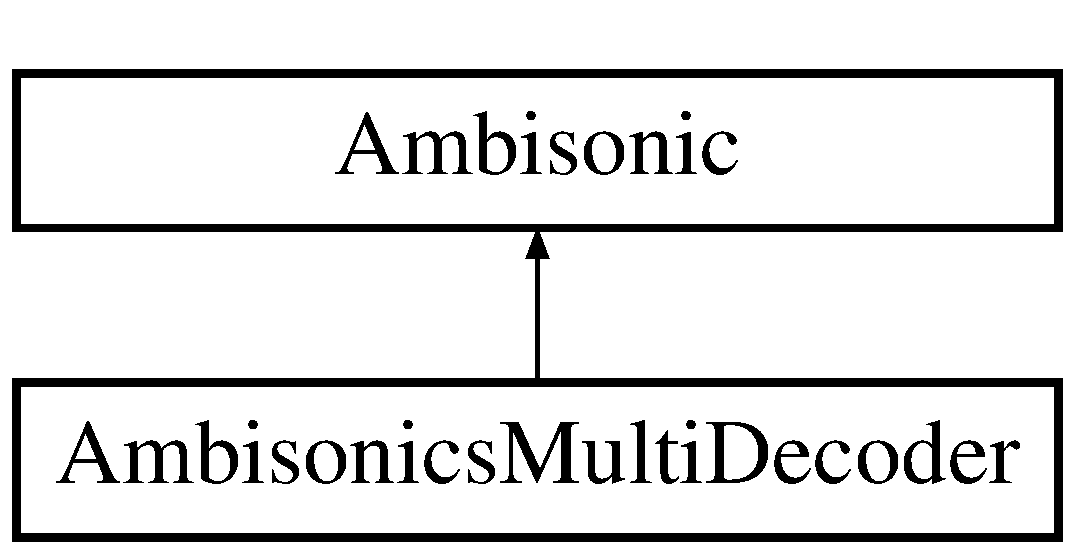
\includegraphics[height=2.000000cm]{class_ambisonics_multi_decoder}
\end{center}
\end{figure}
\subsection*{Public Member Functions}
\begin{DoxyCompactItemize}
\item 
\hyperlink{class_ambisonics_multi_decoder_aa1f1f419fc8b8d032e562009ccb2e6bc}{Ambisonics\-Multi\-Decoder} (long an\-Order=1, long a\-Number\-Of\-Loudspeakers=4, long a\-Mode=Hoa\-\_\-\-Dec\-\_\-\-Ambisonic, long a\-Pinna\-Size=Hoa\-\_\-\-Small, std\-::string a\-Root\-Path=\char`\"{}\char`\"{}, long a\-Vector\-Size=0, long a\-Sampling\-Rate=44100)
\end{DoxyCompactItemize}


\subsection{Detailed Description}


Definition at line 39 of file Ambisonics\-Multi\-Decoder.\-h.



\subsection{Constructor \& Destructor Documentation}
\hypertarget{class_ambisonics_multi_decoder_aa1f1f419fc8b8d032e562009ccb2e6bc}{\index{Ambisonics\-Multi\-Decoder@{Ambisonics\-Multi\-Decoder}!Ambisonics\-Multi\-Decoder@{Ambisonics\-Multi\-Decoder}}
\index{Ambisonics\-Multi\-Decoder@{Ambisonics\-Multi\-Decoder}!AmbisonicsMultiDecoder@{Ambisonics\-Multi\-Decoder}}
\subsubsection[{Ambisonics\-Multi\-Decoder}]{\setlength{\rightskip}{0pt plus 5cm}Ambisonics\-Multi\-Decoder\-::\-Ambisonics\-Multi\-Decoder (
\begin{DoxyParamCaption}
\item[{long}]{an\-Order = {\ttfamily 1}, }
\item[{long}]{a\-Number\-Of\-Loudspeakers = {\ttfamily 4}, }
\item[{long}]{a\-Mode = {\ttfamily Hoa\-\_\-Dec\-\_\-Ambisonic}, }
\item[{long}]{a\-Pinnae\-Size = {\ttfamily Hoa\-\_\-Small}, }
\item[{std\-::string}]{a\-Root\-Path = {\ttfamily \char`\"{}\char`\"{}}, }
\item[{long}]{a\-Vector\-Size = {\ttfamily 0}, }
\item[{long}]{a\-Sampling\-Rate = {\ttfamily 44100}}
\end{DoxyParamCaption}
)}}\label{class_ambisonics_multi_decoder_aa1f1f419fc8b8d032e562009ccb2e6bc}
Hoa\-Library \-: A High Order Ambisonics Library Copyright (c) 2012-\/2013 Julien Colafrancesco, Pierre Guillot, Eliott Paris, C\-I\-C\-M, Universite Paris-\/8. All rights reserved.

Website \-: \href{http://www.mshparisnord.fr/hoalibrary/}{\tt http\-://www.\-mshparisnord.\-fr/hoalibrary/} Contacts \-: \href{mailto:cicm.mshparisnord@gmail.com}{\tt cicm.\-mshparisnord@gmail.\-com}

Redistribution and use in source and binary forms, with or without modification, are permitted provided that the following conditions are met\-:


\begin{DoxyItemize}
\item Redistributions may not be sold, nor may they be used in a commercial product or activity.
\item Redistributions of source code must retain the above copyright notice, this list of conditions and the following disclaimer.
\item Redistributions in binary form must reproduce the above copyright notice, this list of conditions and the following disclaimer in the documentation and/or other materials provided with the distribution.
\item Neither the name of the C\-I\-C\-M nor the names of its contributors may be used to endorse or promote products derived from this software without specific prior written permission.
\end{DoxyItemize}

T\-H\-I\-S S\-O\-F\-T\-W\-A\-R\-E I\-S P\-R\-O\-V\-I\-D\-E\-D B\-Y T\-H\-E C\-O\-P\-Y\-R\-I\-G\-H\-T H\-O\-L\-D\-E\-R\-S A\-N\-D C\-O\-N\-T\-R\-I\-B\-U\-T\-O\-R\-S \char`\"{}\-A\-S I\-S\char`\"{} A\-N\-D A\-N\-Y E\-X\-P\-R\-E\-S\-S O\-R I\-M\-P\-L\-I\-E\-D W\-A\-R\-R\-A\-N\-T\-I\-E\-S, I\-N\-C\-L\-U\-D\-I\-N\-G, B\-U\-T N\-O\-T L\-I\-M\-I\-T\-E\-D T\-O, T\-H\-E I\-M\-P\-L\-I\-E\-D W\-A\-R\-R\-A\-N\-T\-I\-E\-S O\-F M\-E\-R\-C\-H\-A\-N\-T\-A\-B\-I\-L\-I\-T\-Y A\-N\-D F\-I\-T\-N\-E\-S\-S F\-O\-R A P\-A\-R\-T\-I\-C\-U\-L\-A\-R P\-U\-R\-P\-O\-S\-E A\-R\-E D\-I\-S\-C\-L\-A\-I\-M\-E\-D. I\-N N\-O E\-V\-E\-N\-T S\-H\-A\-L\-L T\-H\-E C\-O\-P\-Y\-R\-I\-G\-H\-T H\-O\-L\-D\-E\-R O\-R C\-O\-N\-T\-R\-I\-B\-U\-T\-O\-R\-S B\-E L\-I\-A\-B\-L\-E F\-O\-R A\-N\-Y D\-I\-R\-E\-C\-T, I\-N\-D\-I\-R\-E\-C\-T, I\-N\-C\-I\-D\-E\-N\-T\-A\-L, S\-P\-E\-C\-I\-A\-L, E\-X\-E\-M\-P\-L\-A\-R\-Y, O\-R C\-O\-N\-S\-E\-Q\-U\-E\-N\-T\-I\-A\-L D\-A\-M\-A\-G\-E\-S (I\-N\-C\-L\-U\-D\-I\-N\-G, B\-U\-T N\-O\-T L\-I\-M\-I\-T\-E\-D T\-O, P\-R\-O\-C\-U\-R\-E\-M\-E\-N\-T O\-F S\-U\-B\-S\-T\-I\-T\-U\-T\-E G\-O\-O\-D\-S O\-R S\-E\-R\-V\-I\-C\-E\-S; L\-O\-S\-S O\-F U\-S\-E, D\-A\-T\-A, O\-R P\-R\-O\-F\-I\-T\-S; O\-R B\-U\-S\-I\-N\-E\-S\-S I\-N\-T\-E\-R\-R\-U\-P\-T\-I\-O\-N) H\-O\-W\-E\-V\-E\-R C\-A\-U\-S\-E\-D A\-N\-D O\-N A\-N\-Y T\-H\-E\-O\-R\-Y O\-F L\-I\-A\-B\-I\-L\-I\-T\-Y, W\-H\-E\-T\-H\-E\-R I\-N C\-O\-N\-T\-R\-A\-C\-T, S\-T\-R\-I\-C\-T L\-I\-A\-B\-I\-L\-I\-T\-Y, O\-R T\-O\-R\-T (I\-N\-C\-L\-U\-D\-I\-N\-G N\-E\-G\-L\-I\-G\-E\-N\-C\-E O\-R O\-T\-H\-E\-R\-W\-I\-S\-E) A\-R\-I\-S\-I\-N\-G I\-N A\-N\-Y W\-A\-Y O\-U\-T O\-F T\-H\-E U\-S\-E O\-F T\-H\-I\-S S\-O\-F\-T\-W\-A\-R\-E, E\-V\-E\-N I\-F A\-D\-V\-I\-S\-E\-D O\-F T\-H\-E P\-O\-S\-S\-I\-B\-I\-L\-I\-T\-Y O\-F S\-U\-C\-H D\-A\-M\-A\-G\-E. 

Definition at line 28 of file Ambisonics\-Multi\-Decoder.\-cpp.



The documentation for this class was generated from the following files\-:\begin{DoxyCompactItemize}
\item 
/\-Users/\-Pierre/\-Source\-Tree/\-Hoa\-Library/\-Sources/hoa\-Multi\-Decoder/Ambisonics\-Multi\-Decoder.\-h\item 
/\-Users/\-Pierre/\-Source\-Tree/\-Hoa\-Library/\-Sources/hoa\-Multi\-Decoder/Ambisonics\-Multi\-Decoder.\-cpp\end{DoxyCompactItemize}

\hypertarget{class_ambisonics_multi_maps}{\section{Ambisonics\-Multi\-Maps Class Reference}
\label{class_ambisonics_multi_maps}\index{Ambisonics\-Multi\-Maps@{Ambisonics\-Multi\-Maps}}
}


{\ttfamily \#include $<$Ambisonic\-Multi\-Maps.\-h$>$}

Inheritance diagram for Ambisonics\-Multi\-Maps\-:\begin{figure}[H]
\begin{center}
\leavevmode
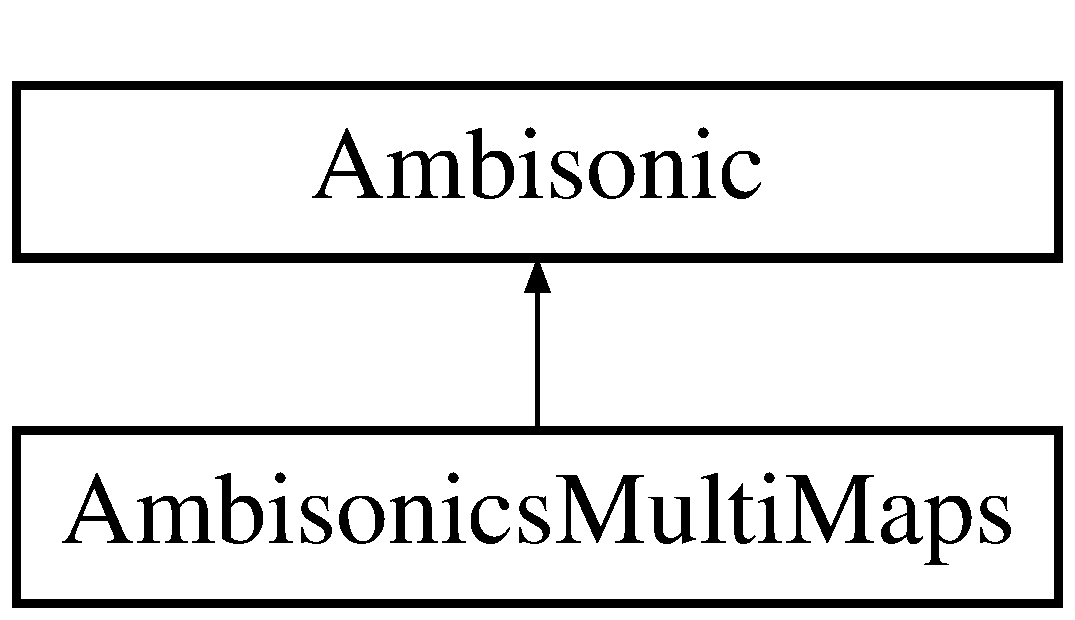
\includegraphics[height=2.000000cm]{class_ambisonics_multi_maps}
\end{center}
\end{figure}
\subsection*{Public Member Functions}
\begin{DoxyCompactItemize}
\item 
\hyperlink{class_ambisonics_multi_maps_a44cd07ce71531668e9f950ef35fc4f74}{Ambisonics\-Multi\-Maps} (long an\-Order=1, long a\-Number\-Of\-Sources=1, long a\-Ramp\-Sample=4410, long a\-Vector\-Size=0, long a\-Sampling\-Rate=0)
\item 
\hypertarget{class_ambisonics_multi_maps_abc7b6728ceae6a4c8e3322a51b1fc6de}{long {\bfseries get\-Number\-Of\-Sources} ()}\label{class_ambisonics_multi_maps_abc7b6728ceae6a4c8e3322a51b1fc6de}

\item 
\hypertarget{class_ambisonics_multi_maps_ad6182a18f461c46f5484ebf06f3cacd5}{long {\bfseries get\-Muted} (long a\-Source\-Index)}\label{class_ambisonics_multi_maps_ad6182a18f461c46f5484ebf06f3cacd5}

\item 
\hypertarget{class_ambisonics_multi_maps_ad763b353e4189018ea90e4056b6b70d5}{double {\bfseries get\-Radius} (long a\-Source\-Index)}\label{class_ambisonics_multi_maps_ad763b353e4189018ea90e4056b6b70d5}

\item 
\hypertarget{class_ambisonics_multi_maps_a7d4f49822ebac5640901d7874458b6dd}{double {\bfseries get\-Azimuth} (long a\-Source\-Index)}\label{class_ambisonics_multi_maps_a7d4f49822ebac5640901d7874458b6dd}

\item 
\hypertarget{class_ambisonics_multi_maps_ad5628dffa6f0db84c0ef586c64ef5528}{long {\bfseries get\-Ramp} ()}\label{class_ambisonics_multi_maps_ad5628dffa6f0db84c0ef586c64ef5528}

\item 
\hypertarget{class_ambisonics_multi_maps_a19e9a91b0249fac400694e9abee5873c}{std\-::string {\bfseries get\-Source\-Name} (long an\-Index)}\label{class_ambisonics_multi_maps_a19e9a91b0249fac400694e9abee5873c}

\item 
\hypertarget{class_ambisonics_multi_maps_aaeab01b8498a639b57cb505afde11550}{void {\bfseries set\-Vector\-Size} (long a\-Vector\-Size)}\label{class_ambisonics_multi_maps_aaeab01b8498a639b57cb505afde11550}

\item 
\hypertarget{class_ambisonics_multi_maps_a544202615489298825be4a5154b9d71b}{void {\bfseries set\-Number\-Of\-Sources} (long a\-Number\-Of\-Sources)}\label{class_ambisonics_multi_maps_a544202615489298825be4a5154b9d71b}

\item 
\hypertarget{class_ambisonics_multi_maps_a0896d78a07c0153b12670b4bd692a29d}{void {\bfseries set\-Coordinates\-Polar} (long a\-Source\-Index, double a\-Radius, double an\-Azimuth)}\label{class_ambisonics_multi_maps_a0896d78a07c0153b12670b4bd692a29d}

\item 
\hypertarget{class_ambisonics_multi_maps_a07adae9006fffcf2e86e2a866117a6f0}{void {\bfseries set\-Coordinates\-Radius} (long a\-Source\-Index, double a\-Radius)}\label{class_ambisonics_multi_maps_a07adae9006fffcf2e86e2a866117a6f0}

\item 
\hypertarget{class_ambisonics_multi_maps_ad8bb7e3bc844e8a5dccca8f5f08c9a36}{void {\bfseries set\-Coordinates\-Azimuth} (long a\-Source\-Index, double an\-Azimuth)}\label{class_ambisonics_multi_maps_ad8bb7e3bc844e8a5dccca8f5f08c9a36}

\item 
\hypertarget{class_ambisonics_multi_maps_a1821484046b0282aec56ce53cf4dcc37}{void {\bfseries set\-Coordinates\-Cartesian} (long a\-Source\-Index, double an\-Abscissa, double an\-Ordinate)}\label{class_ambisonics_multi_maps_a1821484046b0282aec56ce53cf4dcc37}

\item 
\hypertarget{class_ambisonics_multi_maps_af6559d6c5430147c3e3b632a9d16984c}{void {\bfseries set\-Coordinates\-Abscissa} (long a\-Source\-Index, double an\-Abscissa)}\label{class_ambisonics_multi_maps_af6559d6c5430147c3e3b632a9d16984c}

\item 
\hypertarget{class_ambisonics_multi_maps_a8c3a2b27fc3f4b2bcbd82c77d6cd80b7}{void {\bfseries set\-Coordinates\-Ordinate} (long a\-Source\-Index, double an\-Ordinate)}\label{class_ambisonics_multi_maps_a8c3a2b27fc3f4b2bcbd82c77d6cd80b7}

\item 
\hypertarget{class_ambisonics_multi_maps_ab022a734821cfcc08af825eb761c6179}{void {\bfseries set\-Muted} (long a\-Source\-Index, long a\-Value)}\label{class_ambisonics_multi_maps_ab022a734821cfcc08af825eb761c6179}

\item 
\hypertarget{class_ambisonics_multi_maps_ac343b301c27a796e5d081e6e92477cbd}{void {\bfseries set\-Ramp} (long a\-Number\-Of\-Sample)}\label{class_ambisonics_multi_maps_ac343b301c27a796e5d081e6e92477cbd}

\item 
\hypertarget{class_ambisonics_multi_maps_a9661cac4012f4d1df56f378a73075b1f}{void {\bfseries process} (const float $\ast$inputs, float $\ast$outputs)}\label{class_ambisonics_multi_maps_a9661cac4012f4d1df56f378a73075b1f}

\item 
\hypertarget{class_ambisonics_multi_maps_aa955c654fdadaf3f553795a3f6b1211a}{void {\bfseries process} (const double $\ast$inputs, double $\ast$outputs)}\label{class_ambisonics_multi_maps_aa955c654fdadaf3f553795a3f6b1211a}

\item 
\hypertarget{class_ambisonics_multi_maps_aba7d09a43c9991c2205d32af737d6a17}{void {\bfseries process} (const float $\ast$const $\ast$inputs, float $\ast$$\ast$outputs)}\label{class_ambisonics_multi_maps_aba7d09a43c9991c2205d32af737d6a17}

\item 
\hypertarget{class_ambisonics_multi_maps_af1ae8119f22884ed342a627e411990e1}{void {\bfseries process} (const double $\ast$const $\ast$inputs, double $\ast$$\ast$outputs)}\label{class_ambisonics_multi_maps_af1ae8119f22884ed342a627e411990e1}

\item 
\hypertarget{class_ambisonics_multi_maps_a0e80a467c8959d98b6a752e1a89eebb2}{void {\bfseries process\-Cartesian} (float a\-Inputs, float $\ast$a\-Outputs, float an\-Abscissa, float an\-Ordinate)}\label{class_ambisonics_multi_maps_a0e80a467c8959d98b6a752e1a89eebb2}

\item 
\hypertarget{class_ambisonics_multi_maps_a2ac5281bdf765396560ae918e5183916}{void {\bfseries process\-Polar} (float a\-Inputs, float $\ast$a\-Outputs, float a\-Radius, float an\-Azimuth)}\label{class_ambisonics_multi_maps_a2ac5281bdf765396560ae918e5183916}

\item 
\hypertarget{class_ambisonics_multi_maps_a7ee6524be2308c6a0cac03f464d03546}{void {\bfseries process\-Cartesian} (double a\-Inputs, double $\ast$a\-Outputs, double an\-Abscissa, double an\-Ordinate)}\label{class_ambisonics_multi_maps_a7ee6524be2308c6a0cac03f464d03546}

\item 
\hypertarget{class_ambisonics_multi_maps_a4ec92455f3ef2aaa102701ba5bf9b49a}{void {\bfseries process\-Polar} (double a\-Inputs, double $\ast$a\-Outputs, double a\-Radius, double an\-Azimuth)}\label{class_ambisonics_multi_maps_a4ec92455f3ef2aaa102701ba5bf9b49a}

\item 
\hypertarget{class_ambisonics_multi_maps_a7a1506aac60606d11aa75e6c66230d00}{void {\bfseries process\-Radius} (float a\-Inputs, float $\ast$a\-Outputs, float a\-Radius)}\label{class_ambisonics_multi_maps_a7a1506aac60606d11aa75e6c66230d00}

\item 
\hypertarget{class_ambisonics_multi_maps_ad0f68d09fd49dd5b8571dcc6736a301c}{void {\bfseries process\-Azimuth} (float a\-Inputs, float $\ast$a\-Outputs, float an\-Azimuth)}\label{class_ambisonics_multi_maps_ad0f68d09fd49dd5b8571dcc6736a301c}

\item 
\hypertarget{class_ambisonics_multi_maps_a9c47dbd0d4a562785843cd65f6e00988}{void {\bfseries process\-Radius} (double a\-Inputs, double $\ast$a\-Outputs, double a\-Radius)}\label{class_ambisonics_multi_maps_a9c47dbd0d4a562785843cd65f6e00988}

\item 
\hypertarget{class_ambisonics_multi_maps_aca539584e7f3c43043456e08d83987c1}{void {\bfseries process\-Azimuth} (double a\-Inputs, double $\ast$a\-Outputs, double an\-Azimuth)}\label{class_ambisonics_multi_maps_aca539584e7f3c43043456e08d83987c1}

\item 
\hypertarget{class_ambisonics_multi_maps_a785f59b9207bbcfcf02b06489930c345}{void {\bfseries process\-Abscissa} (float a\-Inputs, float $\ast$a\-Outputs, float an\-Abscissa)}\label{class_ambisonics_multi_maps_a785f59b9207bbcfcf02b06489930c345}

\item 
\hypertarget{class_ambisonics_multi_maps_aa46ce576639f7edb38447f61341b8fbb}{void {\bfseries process\-Ordinate} (float a\-Inputs, float $\ast$a\-Outputs, float an\-Ordinate)}\label{class_ambisonics_multi_maps_aa46ce576639f7edb38447f61341b8fbb}

\item 
\hypertarget{class_ambisonics_multi_maps_a759863c671babc71a1006e86341503dc}{void {\bfseries process\-Abscissa} (double a\-Inputs, double $\ast$a\-Outputs, double an\-Abscissa)}\label{class_ambisonics_multi_maps_a759863c671babc71a1006e86341503dc}

\item 
\hypertarget{class_ambisonics_multi_maps_a7b9443f181a3743efd6f5d20c7c36c20}{void {\bfseries process\-Ordinate} (double a\-Inputs, double $\ast$a\-Outputs, double an\-Ordinate)}\label{class_ambisonics_multi_maps_a7b9443f181a3743efd6f5d20c7c36c20}

\item 
\hypertarget{class_ambisonics_multi_maps_a43e20f87b6548d959b68039ae434f18d}{void {\bfseries process\-Cartesian} (float $\ast$a\-Inputs, float $\ast$$\ast$a\-Outputs, float $\ast$an\-Abscissa, float $\ast$an\-Ordinate)}\label{class_ambisonics_multi_maps_a43e20f87b6548d959b68039ae434f18d}

\item 
\hypertarget{class_ambisonics_multi_maps_a986adc7a6d8995d9ac395c7f52ef3d9c}{void {\bfseries process\-Polar} (float $\ast$a\-Inputs, float $\ast$$\ast$a\-Outputs, float $\ast$a\-Radius, float $\ast$an\-Azimuth)}\label{class_ambisonics_multi_maps_a986adc7a6d8995d9ac395c7f52ef3d9c}

\item 
\hypertarget{class_ambisonics_multi_maps_acfa354e1fd81fd6c650e292e5f839611}{void {\bfseries process\-Cartesian} (double $\ast$a\-Inputs, double $\ast$$\ast$a\-Outputs, double $\ast$an\-Abscissa, double $\ast$an\-Ordinate)}\label{class_ambisonics_multi_maps_acfa354e1fd81fd6c650e292e5f839611}

\item 
\hypertarget{class_ambisonics_multi_maps_ab689ee70c21056307ef196ac12d90476}{void {\bfseries process\-Polar} (double $\ast$a\-Inputs, double $\ast$$\ast$a\-Outputs, double $\ast$a\-Radius, double $\ast$an\-Azimuth)}\label{class_ambisonics_multi_maps_ab689ee70c21056307ef196ac12d90476}

\item 
\hypertarget{class_ambisonics_multi_maps_a26f8c22035a34dff197100daae26c5e5}{void {\bfseries process\-Radius} (float $\ast$a\-Inputs, float $\ast$$\ast$a\-Outputs, float $\ast$a\-Radius)}\label{class_ambisonics_multi_maps_a26f8c22035a34dff197100daae26c5e5}

\item 
\hypertarget{class_ambisonics_multi_maps_a0ab8bc9f6938c9632416042ed63fa871}{void {\bfseries process\-Azimuth} (float $\ast$a\-Inputs, float $\ast$$\ast$a\-Outputs, float $\ast$an\-Azimuth)}\label{class_ambisonics_multi_maps_a0ab8bc9f6938c9632416042ed63fa871}

\item 
\hypertarget{class_ambisonics_multi_maps_a61a1cbcd47f04fddcb0124d9e81bef55}{void {\bfseries process\-Radius} (double $\ast$a\-Inputs, double $\ast$$\ast$a\-Outputs, double $\ast$a\-Radius)}\label{class_ambisonics_multi_maps_a61a1cbcd47f04fddcb0124d9e81bef55}

\item 
\hypertarget{class_ambisonics_multi_maps_af4272974aa583e88c9aba336235fb2ec}{void {\bfseries process\-Azimuth} (double $\ast$a\-Inputs, double $\ast$$\ast$a\-Outputs, double $\ast$an\-Azimuth)}\label{class_ambisonics_multi_maps_af4272974aa583e88c9aba336235fb2ec}

\item 
\hypertarget{class_ambisonics_multi_maps_a51869549f420dd06dcf75c7072b4b2d7}{void {\bfseries process\-Abscissa} (float $\ast$a\-Inputs, float $\ast$$\ast$a\-Outputs, float $\ast$an\-Abscissa)}\label{class_ambisonics_multi_maps_a51869549f420dd06dcf75c7072b4b2d7}

\item 
\hypertarget{class_ambisonics_multi_maps_a99e786c532d9bfeabf0a9a0d5998ea72}{void {\bfseries process\-Ordinate} (float $\ast$a\-Inputs, float $\ast$$\ast$a\-Outputs, float $\ast$an\-Ordinate)}\label{class_ambisonics_multi_maps_a99e786c532d9bfeabf0a9a0d5998ea72}

\item 
\hypertarget{class_ambisonics_multi_maps_a02dc73d518ccf8da9f584a3d89705193}{void {\bfseries process\-Abscissa} (double $\ast$a\-Inputs, double $\ast$$\ast$a\-Outputs, double $\ast$an\-Abscissa)}\label{class_ambisonics_multi_maps_a02dc73d518ccf8da9f584a3d89705193}

\item 
\hypertarget{class_ambisonics_multi_maps_a0e73b65563ac00923c44f12c16d55592}{void {\bfseries process\-Ordinate} (double $\ast$a\-Inputs, double $\ast$$\ast$a\-Outputs, double $\ast$an\-Ordinate)}\label{class_ambisonics_multi_maps_a0e73b65563ac00923c44f12c16d55592}

\end{DoxyCompactItemize}
\subsection*{Additional Inherited Members}


\subsection{Detailed Description}
Hoa\-Library \-: A High Order Ambisonics Library Copyright (c) 2012-\/2013 Julien Colafrancesco, Pierre Guillot, Eliott Paris, C\-I\-C\-M, Universite Paris-\/8. All rights reserved.

Website \-: \href{http://www.mshparisnord.fr/hoalibrary/}{\tt http\-://www.\-mshparisnord.\-fr/hoalibrary/} Contacts \-: \href{mailto:cicm.mshparisnord@gmail.com}{\tt cicm.\-mshparisnord@gmail.\-com}

Redistribution and use in source and binary forms, with or without modification, are permitted provided that the following conditions are met\-:


\begin{DoxyItemize}
\item Redistributions may not be sold, nor may they be used in a commercial product or activity.
\item Redistributions of source code must retain the above copyright notice, this list of conditions and the following disclaimer.
\item Redistributions in binary form must reproduce the above copyright notice, this list of conditions and the following disclaimer in the documentation and/or other materials provided with the distribution.
\item Neither the name of the C\-I\-C\-M nor the names of its contributors may be used to endorse or promote products derived from this software without specific prior written permission.
\end{DoxyItemize}

T\-H\-I\-S S\-O\-F\-T\-W\-A\-R\-E I\-S P\-R\-O\-V\-I\-D\-E\-D B\-Y T\-H\-E C\-O\-P\-Y\-R\-I\-G\-H\-T H\-O\-L\-D\-E\-R\-S A\-N\-D C\-O\-N\-T\-R\-I\-B\-U\-T\-O\-R\-S \char`\"{}\-A\-S I\-S\char`\"{} A\-N\-D A\-N\-Y E\-X\-P\-R\-E\-S\-S O\-R I\-M\-P\-L\-I\-E\-D W\-A\-R\-R\-A\-N\-T\-I\-E\-S, I\-N\-C\-L\-U\-D\-I\-N\-G, B\-U\-T N\-O\-T L\-I\-M\-I\-T\-E\-D T\-O, T\-H\-E I\-M\-P\-L\-I\-E\-D W\-A\-R\-R\-A\-N\-T\-I\-E\-S O\-F M\-E\-R\-C\-H\-A\-N\-T\-A\-B\-I\-L\-I\-T\-Y A\-N\-D F\-I\-T\-N\-E\-S\-S F\-O\-R A P\-A\-R\-T\-I\-C\-U\-L\-A\-R P\-U\-R\-P\-O\-S\-E A\-R\-E D\-I\-S\-C\-L\-A\-I\-M\-E\-D. I\-N N\-O E\-V\-E\-N\-T S\-H\-A\-L\-L T\-H\-E C\-O\-P\-Y\-R\-I\-G\-H\-T H\-O\-L\-D\-E\-R O\-R C\-O\-N\-T\-R\-I\-B\-U\-T\-O\-R\-S B\-E L\-I\-A\-B\-L\-E F\-O\-R A\-N\-Y D\-I\-R\-E\-C\-T, I\-N\-D\-I\-R\-E\-C\-T, I\-N\-C\-I\-D\-E\-N\-T\-A\-L, S\-P\-E\-C\-I\-A\-L, E\-X\-E\-M\-P\-L\-A\-R\-Y, O\-R C\-O\-N\-S\-E\-Q\-U\-E\-N\-T\-I\-A\-L D\-A\-M\-A\-G\-E\-S (I\-N\-C\-L\-U\-D\-I\-N\-G, B\-U\-T N\-O\-T L\-I\-M\-I\-T\-E\-D T\-O, P\-R\-O\-C\-U\-R\-E\-M\-E\-N\-T O\-F S\-U\-B\-S\-T\-I\-T\-U\-T\-E G\-O\-O\-D\-S O\-R S\-E\-R\-V\-I\-C\-E\-S; L\-O\-S\-S O\-F U\-S\-E, D\-A\-T\-A, O\-R P\-R\-O\-F\-I\-T\-S; O\-R B\-U\-S\-I\-N\-E\-S\-S I\-N\-T\-E\-R\-R\-U\-P\-T\-I\-O\-N) H\-O\-W\-E\-V\-E\-R C\-A\-U\-S\-E\-D A\-N\-D O\-N A\-N\-Y T\-H\-E\-O\-R\-Y O\-F L\-I\-A\-B\-I\-L\-I\-T\-Y, W\-H\-E\-T\-H\-E\-R I\-N C\-O\-N\-T\-R\-A\-C\-T, S\-T\-R\-I\-C\-T L\-I\-A\-B\-I\-L\-I\-T\-Y, O\-R T\-O\-R\-T (I\-N\-C\-L\-U\-D\-I\-N\-G N\-E\-G\-L\-I\-G\-E\-N\-C\-E O\-R O\-T\-H\-E\-R\-W\-I\-S\-E) A\-R\-I\-S\-I\-N\-G I\-N A\-N\-Y W\-A\-Y O\-U\-T O\-F T\-H\-E U\-S\-E O\-F T\-H\-I\-S S\-O\-F\-T\-W\-A\-R\-E, E\-V\-E\-N I\-F A\-D\-V\-I\-S\-E\-D O\-F T\-H\-E P\-O\-S\-S\-I\-B\-I\-L\-I\-T\-Y O\-F S\-U\-C\-H D\-A\-M\-A\-G\-E. 

\subsection{Constructor \& Destructor Documentation}
\hypertarget{class_ambisonics_multi_maps_a44cd07ce71531668e9f950ef35fc4f74}{\index{Ambisonics\-Multi\-Maps@{Ambisonics\-Multi\-Maps}!Ambisonics\-Multi\-Maps@{Ambisonics\-Multi\-Maps}}
\index{Ambisonics\-Multi\-Maps@{Ambisonics\-Multi\-Maps}!AmbisonicsMultiMaps@{Ambisonics\-Multi\-Maps}}
\subsubsection[{Ambisonics\-Multi\-Maps}]{\setlength{\rightskip}{0pt plus 5cm}Ambisonics\-Multi\-Maps\-::\-Ambisonics\-Multi\-Maps (
\begin{DoxyParamCaption}
\item[{long}]{an\-Order = {\ttfamily 1}, }
\item[{long}]{a\-Number\-Of\-Sources = {\ttfamily 1}, }
\item[{long}]{a\-Ramp\-Sample = {\ttfamily 4410}, }
\item[{long}]{a\-Vector\-Size = {\ttfamily 0}, }
\item[{long}]{a\-Sampling\-Rate = {\ttfamily 0}}
\end{DoxyParamCaption}
)}}\label{class_ambisonics_multi_maps_a44cd07ce71531668e9f950ef35fc4f74}
Hoa\-Library \-: A High Order Ambisonics Library Copyright (c) 2012-\/2013 Julien Colafrancesco, Pierre Guillot, Eliott Paris, C\-I\-C\-M, Universite Paris-\/8. All rights reserved.

Website \-: \href{http://www.mshparisnord.fr/hoalibrary/}{\tt http\-://www.\-mshparisnord.\-fr/hoalibrary/} Contacts \-: \href{mailto:cicm.mshparisnord@gmail.com}{\tt cicm.\-mshparisnord@gmail.\-com}

Redistribution and use in source and binary forms, with or without modification, are permitted provided that the following conditions are met\-:


\begin{DoxyItemize}
\item Redistributions may not be sold, nor may they be used in a commercial product or activity.
\item Redistributions of source code must retain the above copyright notice, this list of conditions and the following disclaimer.
\item Redistributions in binary form must reproduce the above copyright notice, this list of conditions and the following disclaimer in the documentation and/or other materials provided with the distribution.
\item Neither the name of the C\-I\-C\-M nor the names of its contributors may be used to endorse or promote products derived from this software without specific prior written permission.
\end{DoxyItemize}

T\-H\-I\-S S\-O\-F\-T\-W\-A\-R\-E I\-S P\-R\-O\-V\-I\-D\-E\-D B\-Y T\-H\-E C\-O\-P\-Y\-R\-I\-G\-H\-T H\-O\-L\-D\-E\-R\-S A\-N\-D C\-O\-N\-T\-R\-I\-B\-U\-T\-O\-R\-S \char`\"{}\-A\-S I\-S\char`\"{} A\-N\-D A\-N\-Y E\-X\-P\-R\-E\-S\-S O\-R I\-M\-P\-L\-I\-E\-D W\-A\-R\-R\-A\-N\-T\-I\-E\-S, I\-N\-C\-L\-U\-D\-I\-N\-G, B\-U\-T N\-O\-T L\-I\-M\-I\-T\-E\-D T\-O, T\-H\-E I\-M\-P\-L\-I\-E\-D W\-A\-R\-R\-A\-N\-T\-I\-E\-S O\-F M\-E\-R\-C\-H\-A\-N\-T\-A\-B\-I\-L\-I\-T\-Y A\-N\-D F\-I\-T\-N\-E\-S\-S F\-O\-R A P\-A\-R\-T\-I\-C\-U\-L\-A\-R P\-U\-R\-P\-O\-S\-E A\-R\-E D\-I\-S\-C\-L\-A\-I\-M\-E\-D. I\-N N\-O E\-V\-E\-N\-T S\-H\-A\-L\-L T\-H\-E C\-O\-P\-Y\-R\-I\-G\-H\-T H\-O\-L\-D\-E\-R O\-R C\-O\-N\-T\-R\-I\-B\-U\-T\-O\-R\-S B\-E L\-I\-A\-B\-L\-E F\-O\-R A\-N\-Y D\-I\-R\-E\-C\-T, I\-N\-D\-I\-R\-E\-C\-T, I\-N\-C\-I\-D\-E\-N\-T\-A\-L, S\-P\-E\-C\-I\-A\-L, E\-X\-E\-M\-P\-L\-A\-R\-Y, O\-R C\-O\-N\-S\-E\-Q\-U\-E\-N\-T\-I\-A\-L D\-A\-M\-A\-G\-E\-S (I\-N\-C\-L\-U\-D\-I\-N\-G, B\-U\-T N\-O\-T L\-I\-M\-I\-T\-E\-D T\-O, P\-R\-O\-C\-U\-R\-E\-M\-E\-N\-T O\-F S\-U\-B\-S\-T\-I\-T\-U\-T\-E G\-O\-O\-D\-S O\-R S\-E\-R\-V\-I\-C\-E\-S; L\-O\-S\-S O\-F U\-S\-E, D\-A\-T\-A, O\-R P\-R\-O\-F\-I\-T\-S; O\-R B\-U\-S\-I\-N\-E\-S\-S I\-N\-T\-E\-R\-R\-U\-P\-T\-I\-O\-N) H\-O\-W\-E\-V\-E\-R C\-A\-U\-S\-E\-D A\-N\-D O\-N A\-N\-Y T\-H\-E\-O\-R\-Y O\-F L\-I\-A\-B\-I\-L\-I\-T\-Y, W\-H\-E\-T\-H\-E\-R I\-N C\-O\-N\-T\-R\-A\-C\-T, S\-T\-R\-I\-C\-T L\-I\-A\-B\-I\-L\-I\-T\-Y, O\-R T\-O\-R\-T (I\-N\-C\-L\-U\-D\-I\-N\-G N\-E\-G\-L\-I\-G\-E\-N\-C\-E O\-R O\-T\-H\-E\-R\-W\-I\-S\-E) A\-R\-I\-S\-I\-N\-G I\-N A\-N\-Y W\-A\-Y O\-U\-T O\-F T\-H\-E U\-S\-E O\-F T\-H\-I\-S S\-O\-F\-T\-W\-A\-R\-E, E\-V\-E\-N I\-F A\-D\-V\-I\-S\-E\-D O\-F T\-H\-E P\-O\-S\-S\-I\-B\-I\-L\-I\-T\-Y O\-F S\-U\-C\-H D\-A\-M\-A\-G\-E. 

The documentation for this class was generated from the following files\-:\begin{DoxyCompactItemize}
\item 
/\-Users/\-Pierre/\-Source\-Tree/\-Hoa\-Library/\-Sources/hoa\-Map/Ambisonic\-Multi\-Maps.\-h\item 
/\-Users/\-Pierre/\-Source\-Tree/\-Hoa\-Library/\-Sources/hoa\-Map/Ambisonic\-Multi\-Maps.\-cpp\end{DoxyCompactItemize}

\hypertarget{class_ambisonic_space}{\section{Ambisonic\-Space Class Reference}
\label{class_ambisonic_space}\index{Ambisonic\-Space@{Ambisonic\-Space}}
}
Inheritance diagram for Ambisonic\-Space\-:\begin{figure}[H]
\begin{center}
\leavevmode
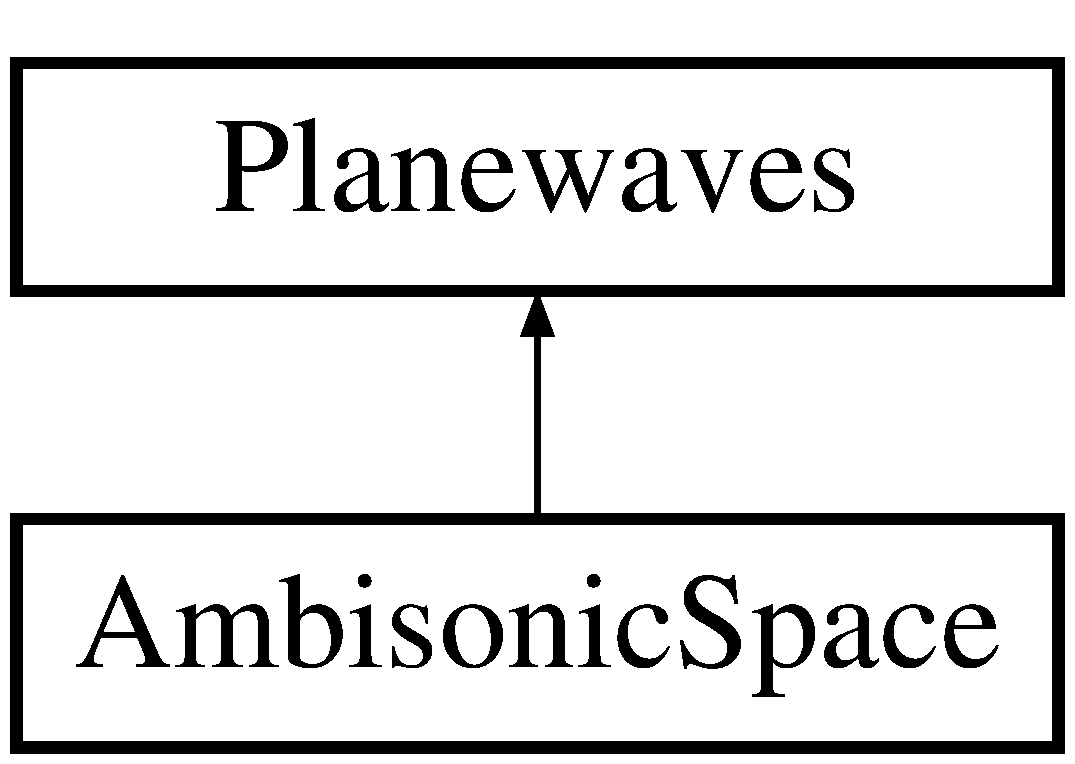
\includegraphics[height=2.000000cm]{class_ambisonic_space}
\end{center}
\end{figure}
\subsection*{Public Member Functions}
\begin{DoxyCompactItemize}
\item 
\hyperlink{class_ambisonic_space_ae68da0697f53d7571c60fc42cc2325ac}{Ambisonic\-Space} (long a\-Number\-Of\-Loudspeakers, long a\-Vector\-Size=0, long a\-Sampling\-Rate=44100)
\item 
\hypertarget{class_ambisonic_space_a8ead71c1496a8d6aedfc7d556c893eef}{double {\bfseries get\-Coefficient} (long an\-Index)}\label{class_ambisonic_space_a8ead71c1496a8d6aedfc7d556c893eef}

\item 
\hypertarget{class_ambisonic_space_a40647ad478fc03f52cee8f6c6e53d9e6}{long {\bfseries get\-Ramp\-In\-Sample} ()}\label{class_ambisonic_space_a40647ad478fc03f52cee8f6c6e53d9e6}

\item 
\hypertarget{class_ambisonic_space_af4f37bedbb6d475b43ccc1cb2fc521cc}{double {\bfseries get\-Ramp\-In\-Ms} ()}\label{class_ambisonic_space_af4f37bedbb6d475b43ccc1cb2fc521cc}

\item 
\hypertarget{class_ambisonic_space_a5263705cddcb592609a8d4bd065c51a7}{void {\bfseries set\-Coefficient} (long an\-Index, double a\-Coefficient)}\label{class_ambisonic_space_a5263705cddcb592609a8d4bd065c51a7}

\item 
\hypertarget{class_ambisonic_space_ad10e02e085175c9f4bf93be4a7dc44da}{void {\bfseries set\-Coefficient} (double $\ast$a\-Coefficient\-Vector)}\label{class_ambisonic_space_ad10e02e085175c9f4bf93be4a7dc44da}

\item 
\hypertarget{class_ambisonic_space_acedc50bcebd09b818fb993e7501b9c9c}{void {\bfseries set\-Coefficient} (float $\ast$a\-Coefficient\-Vector)}\label{class_ambisonic_space_acedc50bcebd09b818fb993e7501b9c9c}

\item 
\hypertarget{class_ambisonic_space_af61e5bffdde94728149fed34df27b014}{void {\bfseries set\-Ramp\-In\-Sample} (long a\-Time\-In\-Sample)}\label{class_ambisonic_space_af61e5bffdde94728149fed34df27b014}

\item 
\hypertarget{class_ambisonic_space_a1bb106fbd02420e8aaf94aad137d11ee}{void {\bfseries set\-Ramp\-In\-Ms} (double a\-Time\-In\-Ms)}\label{class_ambisonic_space_a1bb106fbd02420e8aaf94aad137d11ee}

\item 
\hypertarget{class_ambisonic_space_a7dd6c1c36388986611596163cd0ec733}{void {\bfseries set\-Vector\-Size} (long a\-Vector\-Size)}\label{class_ambisonic_space_a7dd6c1c36388986611596163cd0ec733}

\item 
\hypertarget{class_ambisonic_space_aaee75c804b66e825418ceb0c48e27381}{void {\bfseries set\-Sampling\-Rate} (long a\-Sampling\-Rate)}\label{class_ambisonic_space_aaee75c804b66e825418ceb0c48e27381}

\item 
\hypertarget{class_ambisonic_space_a4e2eb2a2c3ac8bb61495eac9eb3abfde}{void {\bfseries set\-Number\-Of\-Loudspeakers} (long a\-Number\-Of\-Loudspeakers, bool standard\-On\-Off=0)}\label{class_ambisonic_space_a4e2eb2a2c3ac8bb61495eac9eb3abfde}

\item 
\hypertarget{class_ambisonic_space_a88d51fd835645f4f8022e0aefe10bba3}{void {\bfseries process} (const double $\ast$inputs, double $\ast$outputs)}\label{class_ambisonic_space_a88d51fd835645f4f8022e0aefe10bba3}

\item 
\hypertarget{class_ambisonic_space_a248fa89187126c1e1418dc226a10bfb3}{void {\bfseries process} (const float $\ast$inputs, float $\ast$outputs)}\label{class_ambisonic_space_a248fa89187126c1e1418dc226a10bfb3}

\item 
\hypertarget{class_ambisonic_space_a24e370a2161059c11a89771379e38f36}{void {\bfseries process} (double $\ast$io\-Vector)}\label{class_ambisonic_space_a24e370a2161059c11a89771379e38f36}

\item 
\hypertarget{class_ambisonic_space_a94edbc488961063d9ee2927d308df2ea}{void {\bfseries process} (float $\ast$io\-Vector)}\label{class_ambisonic_space_a94edbc488961063d9ee2927d308df2ea}

\item 
\hypertarget{class_ambisonic_space_a28eab2ca744e0a172c17276c0b4b18a1}{void {\bfseries process} (const double $\ast$const $\ast$inputs, double $\ast$$\ast$outputs)}\label{class_ambisonic_space_a28eab2ca744e0a172c17276c0b4b18a1}

\item 
\hypertarget{class_ambisonic_space_ad29fd8d27c7412e20c708b0f00e0a37c}{void {\bfseries process} (const float $\ast$const $\ast$inputs, float $\ast$$\ast$outputs)}\label{class_ambisonic_space_ad29fd8d27c7412e20c708b0f00e0a37c}

\item 
\hypertarget{class_ambisonic_space_aefeb1c2988d73d16de4ee1403f4d566a}{void {\bfseries process} (double $\ast$$\ast$io\-Vectors)}\label{class_ambisonic_space_aefeb1c2988d73d16de4ee1403f4d566a}

\item 
\hypertarget{class_ambisonic_space_a1e5ce921410a6e086ff1a3ce98288f2c}{void {\bfseries process} (float $\ast$$\ast$io\-Vectors)}\label{class_ambisonic_space_a1e5ce921410a6e086ff1a3ce98288f2c}

\end{DoxyCompactItemize}
\subsection*{Additional Inherited Members}


\subsection{Constructor \& Destructor Documentation}
\hypertarget{class_ambisonic_space_ae68da0697f53d7571c60fc42cc2325ac}{\index{Ambisonic\-Space@{Ambisonic\-Space}!Ambisonic\-Space@{Ambisonic\-Space}}
\index{Ambisonic\-Space@{Ambisonic\-Space}!AmbisonicSpace@{Ambisonic\-Space}}
\subsubsection[{Ambisonic\-Space}]{\setlength{\rightskip}{0pt plus 5cm}Ambisonic\-Space\-::\-Ambisonic\-Space (
\begin{DoxyParamCaption}
\item[{long}]{a\-Number\-Of\-Loudspeakers, }
\item[{long}]{a\-Vector\-Size = {\ttfamily 0}, }
\item[{long}]{a\-Sampling\-Rate = {\ttfamily 44100}}
\end{DoxyParamCaption}
)}}\label{class_ambisonic_space_ae68da0697f53d7571c60fc42cc2325ac}
Hoa\-Library \-: A High Order Ambisonics Library Copyright (c) 2012-\/2013 Julien Colafrancesco, Pierre Guillot, Eliott Paris, C\-I\-C\-M, Universite Paris-\/8. All rights reserved.

Website \-: \href{http://www.mshparisnord.fr/hoalibrary/}{\tt http\-://www.\-mshparisnord.\-fr/hoalibrary/} Contacts \-: \href{mailto:cicm.mshparisnord@gmail.com}{\tt cicm.\-mshparisnord@gmail.\-com}

Redistribution and use in source and binary forms, with or without modification, are permitted provided that the following conditions are met\-:


\begin{DoxyItemize}
\item Redistributions may not be sold, nor may they be used in a commercial product or activity.
\item Redistributions of source code must retain the above copyright notice, this list of conditions and the following disclaimer.
\item Redistributions in binary form must reproduce the above copyright notice, this list of conditions and the following disclaimer in the documentation and/or other materials provided with the distribution.
\item Neither the name of the C\-I\-C\-M nor the names of its contributors may be used to endorse or promote products derived from this software without specific prior written permission.
\end{DoxyItemize}

T\-H\-I\-S S\-O\-F\-T\-W\-A\-R\-E I\-S P\-R\-O\-V\-I\-D\-E\-D B\-Y T\-H\-E C\-O\-P\-Y\-R\-I\-G\-H\-T H\-O\-L\-D\-E\-R\-S A\-N\-D C\-O\-N\-T\-R\-I\-B\-U\-T\-O\-R\-S \char`\"{}\-A\-S I\-S\char`\"{} A\-N\-D A\-N\-Y E\-X\-P\-R\-E\-S\-S O\-R I\-M\-P\-L\-I\-E\-D W\-A\-R\-R\-A\-N\-T\-I\-E\-S, I\-N\-C\-L\-U\-D\-I\-N\-G, B\-U\-T N\-O\-T L\-I\-M\-I\-T\-E\-D T\-O, T\-H\-E I\-M\-P\-L\-I\-E\-D W\-A\-R\-R\-A\-N\-T\-I\-E\-S O\-F M\-E\-R\-C\-H\-A\-N\-T\-A\-B\-I\-L\-I\-T\-Y A\-N\-D F\-I\-T\-N\-E\-S\-S F\-O\-R A P\-A\-R\-T\-I\-C\-U\-L\-A\-R P\-U\-R\-P\-O\-S\-E A\-R\-E D\-I\-S\-C\-L\-A\-I\-M\-E\-D. I\-N N\-O E\-V\-E\-N\-T S\-H\-A\-L\-L T\-H\-E C\-O\-P\-Y\-R\-I\-G\-H\-T H\-O\-L\-D\-E\-R O\-R C\-O\-N\-T\-R\-I\-B\-U\-T\-O\-R\-S B\-E L\-I\-A\-B\-L\-E F\-O\-R A\-N\-Y D\-I\-R\-E\-C\-T, I\-N\-D\-I\-R\-E\-C\-T, I\-N\-C\-I\-D\-E\-N\-T\-A\-L, S\-P\-E\-C\-I\-A\-L, E\-X\-E\-M\-P\-L\-A\-R\-Y, O\-R C\-O\-N\-S\-E\-Q\-U\-E\-N\-T\-I\-A\-L D\-A\-M\-A\-G\-E\-S (I\-N\-C\-L\-U\-D\-I\-N\-G, B\-U\-T N\-O\-T L\-I\-M\-I\-T\-E\-D T\-O, P\-R\-O\-C\-U\-R\-E\-M\-E\-N\-T O\-F S\-U\-B\-S\-T\-I\-T\-U\-T\-E G\-O\-O\-D\-S O\-R S\-E\-R\-V\-I\-C\-E\-S; L\-O\-S\-S O\-F U\-S\-E, D\-A\-T\-A, O\-R P\-R\-O\-F\-I\-T\-S; O\-R B\-U\-S\-I\-N\-E\-S\-S I\-N\-T\-E\-R\-R\-U\-P\-T\-I\-O\-N) H\-O\-W\-E\-V\-E\-R C\-A\-U\-S\-E\-D A\-N\-D O\-N A\-N\-Y T\-H\-E\-O\-R\-Y O\-F L\-I\-A\-B\-I\-L\-I\-T\-Y, W\-H\-E\-T\-H\-E\-R I\-N C\-O\-N\-T\-R\-A\-C\-T, S\-T\-R\-I\-C\-T L\-I\-A\-B\-I\-L\-I\-T\-Y, O\-R T\-O\-R\-T (I\-N\-C\-L\-U\-D\-I\-N\-G N\-E\-G\-L\-I\-G\-E\-N\-C\-E O\-R O\-T\-H\-E\-R\-W\-I\-S\-E) A\-R\-I\-S\-I\-N\-G I\-N A\-N\-Y W\-A\-Y O\-U\-T O\-F T\-H\-E U\-S\-E O\-F T\-H\-I\-S S\-O\-F\-T\-W\-A\-R\-E, E\-V\-E\-N I\-F A\-D\-V\-I\-S\-E\-D O\-F T\-H\-E P\-O\-S\-S\-I\-B\-I\-L\-I\-T\-Y O\-F S\-U\-C\-H D\-A\-M\-A\-G\-E. 

The documentation for this class was generated from the following files\-:\begin{DoxyCompactItemize}
\item 
/\-Users/\-Pierre/\-Source\-Tree/\-Hoa\-Library/\-Sources/hoa\-Space/Ambisonic\-Space.\-h\item 
/\-Users/\-Pierre/\-Source\-Tree/\-Hoa\-Library/\-Sources/hoa\-Space/Ambisonic\-Space.\-cpp\end{DoxyCompactItemize}

\hypertarget{class_ambisonic_spectrum}{\section{Ambisonic\-Spectrum Class Reference}
\label{class_ambisonic_spectrum}\index{Ambisonic\-Spectrum@{Ambisonic\-Spectrum}}
}


{\ttfamily \#include $<$Ambisonic\-Spectrum.\-h$>$}

Inheritance diagram for Ambisonic\-Spectrum\-:\begin{figure}[H]
\begin{center}
\leavevmode
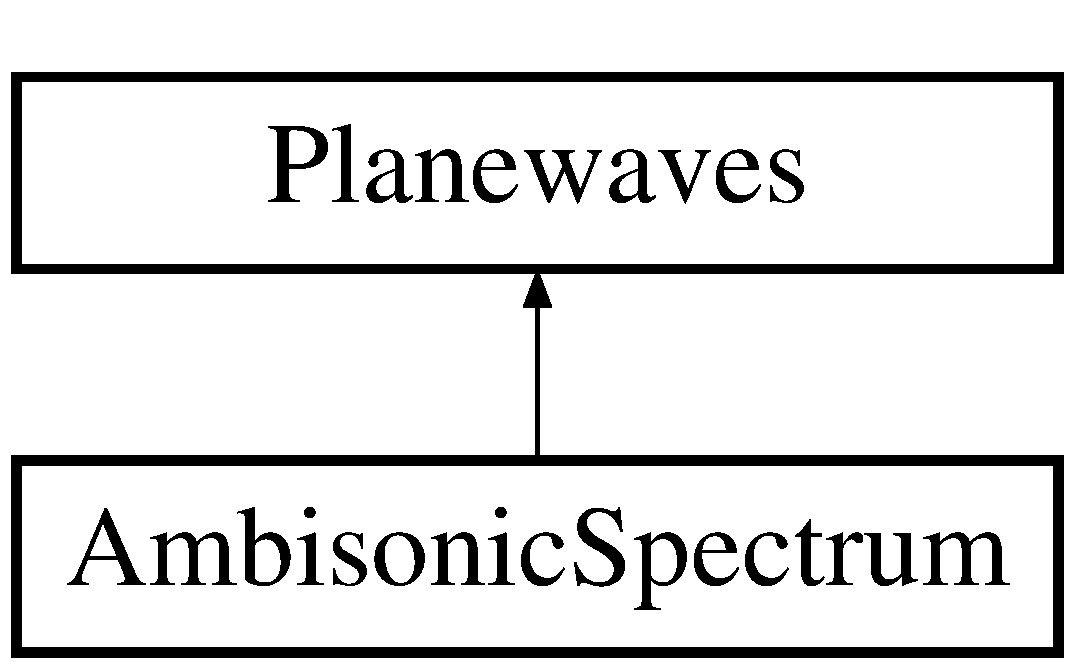
\includegraphics[height=2.000000cm]{class_ambisonic_spectrum}
\end{center}
\end{figure}
\subsection*{Public Member Functions}
\begin{DoxyCompactItemize}
\item 
\hyperlink{class_ambisonic_spectrum_a657f2c97aaab215e95c41f4d07dc8f45}{Ambisonic\-Spectrum} (long a\-Number\-Of\-Loudspeakers=1, long a\-Number\-Of\-Bands=3, long a\-Vector\-Size=0, long a\-Sampling\-Rate=44100)
\item 
\hypertarget{class_ambisonic_spectrum_a67322d6da539d8804711830108289890}{void {\bfseries set\-Number\-Of\-Loudspeakers} (long a\-Number\-Of\-Loudspeakers, bool standard\-On\-Off=0)}\label{class_ambisonic_spectrum_a67322d6da539d8804711830108289890}

\item 
\hypertarget{class_ambisonic_spectrum_a35509a66a23a341cb3fe8db5509cd60c}{void {\bfseries set\-Loudspeaker\-Angle} (long an\-Index, double an\-Angle)}\label{class_ambisonic_spectrum_a35509a66a23a341cb3fe8db5509cd60c}

\item 
\hypertarget{class_ambisonic_spectrum_ae50e8aebafb67fc1883b1b4343c69018}{void {\bfseries set\-Frequency\-Band} (long an\-Index, double a\-Frequency)}\label{class_ambisonic_spectrum_ae50e8aebafb67fc1883b1b4343c69018}

\item 
\hypertarget{class_ambisonic_spectrum_a21fb69a71c815e1ab5bf350668b5dc0c}{void {\bfseries set\-Number\-Of\-Bands} (long a\-Number\-Of\-Bands)}\label{class_ambisonic_spectrum_a21fb69a71c815e1ab5bf350668b5dc0c}

\item 
\hypertarget{class_ambisonic_spectrum_abde7474b423c03a64a4f810dac2805c6}{double {\bfseries get\-Amplitude} (long a\-Band\-Index)}\label{class_ambisonic_spectrum_abde7474b423c03a64a4f810dac2805c6}

\item 
\hypertarget{class_ambisonic_spectrum_a2c98b11e9e41def8f7d6e24ef34a144c}{double {\bfseries get\-Abscissa} (long a\-Band\-Index)}\label{class_ambisonic_spectrum_a2c98b11e9e41def8f7d6e24ef34a144c}

\item 
\hypertarget{class_ambisonic_spectrum_a7d91f3340282b610dca8f5d6133029f5}{double {\bfseries get\-Ordinate} (long a\-Band\-Index)}\label{class_ambisonic_spectrum_a7d91f3340282b610dca8f5d6133029f5}

\item 
\hypertarget{class_ambisonic_spectrum_a05b2917412c783f96af3300c6b93a615}{double {\bfseries get\-Radius} (long a\-Band\-Index)}\label{class_ambisonic_spectrum_a05b2917412c783f96af3300c6b93a615}

\item 
\hypertarget{class_ambisonic_spectrum_a5db3862c241c1803091a180f95151b4d}{double {\bfseries get\-Angle} (long a\-Band\-Index)}\label{class_ambisonic_spectrum_a5db3862c241c1803091a180f95151b4d}

\item 
\hypertarget{class_ambisonic_spectrum_a6c4d7db26791c55b063cb6e096c199c0}{double {\bfseries get\-Log\-Amplitude} (long a\-Band\-Index)}\label{class_ambisonic_spectrum_a6c4d7db26791c55b063cb6e096c199c0}

\item 
\hypertarget{class_ambisonic_spectrum_a5a0194caed12270647a345052c17ca14}{double {\bfseries get\-Log\-Abscissa} (long a\-Band\-Index)}\label{class_ambisonic_spectrum_a5a0194caed12270647a345052c17ca14}

\item 
\hypertarget{class_ambisonic_spectrum_a8e63b1e2663ee142ff51c31b57028ba2}{double {\bfseries get\-Log\-Ordinate} (long a\-Band\-Index)}\label{class_ambisonic_spectrum_a8e63b1e2663ee142ff51c31b57028ba2}

\item 
\hypertarget{class_ambisonic_spectrum_a24d7d8d26f1f5257fe684babc648f6c6}{double {\bfseries get\-Log\-Radius} (long a\-Band\-Index)}\label{class_ambisonic_spectrum_a24d7d8d26f1f5257fe684babc648f6c6}

\item 
\hypertarget{class_ambisonic_spectrum_a65e453f0de97f94d09dd5af107b711e2}{double {\bfseries get\-Log\-Angle} (long a\-Band\-Index)}\label{class_ambisonic_spectrum_a65e453f0de97f94d09dd5af107b711e2}

\item 
\hypertarget{class_ambisonic_spectrum_a85d13a81ce2d971465a0715e9889126f}{double {\bfseries get\-Frequency\-Band} (long an\-Index)}\label{class_ambisonic_spectrum_a85d13a81ce2d971465a0715e9889126f}

\item 
\hypertarget{class_ambisonic_spectrum_a0982fde433c0a1f2d0cbb22340e0c756}{long {\bfseries get\-Number\-Of\-Bands} ()}\label{class_ambisonic_spectrum_a0982fde433c0a1f2d0cbb22340e0c756}

\item 
\hypertarget{class_ambisonic_spectrum_a83e25eaf71ec3cd3c37b0f74af778dcd}{void {\bfseries set\-Vector\-Size} (long a\-Vector\-Size)}\label{class_ambisonic_spectrum_a83e25eaf71ec3cd3c37b0f74af778dcd}

\item 
\hypertarget{class_ambisonic_spectrum_a7bd00bbe40241407a84ea6dc8c5df1bd}{void {\bfseries set\-Sampling\-Rate} (long a\-Sampling\-Rate)}\label{class_ambisonic_spectrum_a7bd00bbe40241407a84ea6dc8c5df1bd}

\item 
\hypertarget{class_ambisonic_spectrum_aec69f768c208a83f5ce55268b942ca1a}{void {\bfseries process} (const double $\ast$const $\ast$inputs)}\label{class_ambisonic_spectrum_aec69f768c208a83f5ce55268b942ca1a}

\item 
\hypertarget{class_ambisonic_spectrum_ab3ab5df934defcaa6e86502f61589b21}{void {\bfseries tick} ()}\label{class_ambisonic_spectrum_ab3ab5df934defcaa6e86502f61589b21}

\end{DoxyCompactItemize}
\subsection*{Additional Inherited Members}


\subsection{Detailed Description}
Hoa\-Library \-: A High Order Ambisonics Library Copyright (c) 2012-\/2013 Julien Colafrancesco, Pierre Guillot, Eliott Paris, C\-I\-C\-M, Universite Paris-\/8. All rights reserved.\-re Guillot, C\-I\-C\-M -\/ Université Paris 8 All rights reserved.

Website \-: \href{http://www.mshparisnord.fr/HoaLibrary/}{\tt http\-://www.\-mshparisnord.\-fr/\-Hoa\-Library/} Contacts \-: \href{mailto:cicm.mshparisnord@gmail.com}{\tt cicm.\-mshparisnord@gmail.\-com}

This file is part of H\-O\-A L\-I\-B\-R\-A\-R\-Y.

H\-O\-A L\-I\-B\-R\-A\-R\-Y is free software\-: you can redistribute it and/or modify it under the terms of the G\-N\-U General Public License as published by the Free Software Foundation, either version 3 of the License, or (at your option) any later version.

This program is distributed in the hope that it will be useful, but W\-I\-T\-H\-O\-U\-T A\-N\-Y W\-A\-R\-R\-A\-N\-T\-Y; without even the implied warranty of M\-E\-R\-C\-H\-A\-N\-T\-A\-B\-I\-L\-I\-T\-Y or F\-I\-T\-N\-E\-S\-S F\-O\-R A P\-A\-R\-T\-I\-C\-U\-L\-A\-R P\-U\-R\-P\-O\-S\-E. See the G\-N\-U General Public License for more details.

You should have received a copy of the G\-N\-U General Public License along with this program. If not, see \href{http://www.gnu.org/licenses/}{\tt http\-://www.\-gnu.\-org/licenses/}. 

\subsection{Constructor \& Destructor Documentation}
\hypertarget{class_ambisonic_spectrum_a657f2c97aaab215e95c41f4d07dc8f45}{\index{Ambisonic\-Spectrum@{Ambisonic\-Spectrum}!Ambisonic\-Spectrum@{Ambisonic\-Spectrum}}
\index{Ambisonic\-Spectrum@{Ambisonic\-Spectrum}!AmbisonicSpectrum@{Ambisonic\-Spectrum}}
\subsubsection[{Ambisonic\-Spectrum}]{\setlength{\rightskip}{0pt plus 5cm}Ambisonic\-Spectrum\-::\-Ambisonic\-Spectrum (
\begin{DoxyParamCaption}
\item[{long}]{a\-Number\-Of\-Loudspeakers = {\ttfamily 1}, }
\item[{long}]{a\-Number\-Of\-Bands = {\ttfamily 3}, }
\item[{long}]{a\-Vector\-Size = {\ttfamily 0}, }
\item[{long}]{a\-Sampling\-Rate = {\ttfamily 44100}}
\end{DoxyParamCaption}
)}}\label{class_ambisonic_spectrum_a657f2c97aaab215e95c41f4d07dc8f45}
Hoa\-Library \-: A High Order Ambisonics Library Copyright (c) 2012-\/2013 Julien Colafrancesco, Pierre Guillot, Eliott Paris, C\-I\-C\-M, Universite Paris-\/8. All rights reserved.\-re Guillot, C\-I\-C\-M -\/ Université Paris 8 All rights reserved.

Website \-: \href{http://www.mshparisnord.fr/HoaLibrary/}{\tt http\-://www.\-mshparisnord.\-fr/\-Hoa\-Library/} Contacts \-: \href{mailto:cicm.mshparisnord@gmail.com}{\tt cicm.\-mshparisnord@gmail.\-com}

This file is part of H\-O\-A L\-I\-B\-R\-A\-R\-Y.

H\-O\-A L\-I\-B\-R\-A\-R\-Y is free software\-: you can redistribute it and/or modify it under the terms of the G\-N\-U General Public License as published by the Free Software Foundation, either version 3 of the License, or (at your option) any later version.

This program is distributed in the hope that it will be useful, but W\-I\-T\-H\-O\-U\-T A\-N\-Y W\-A\-R\-R\-A\-N\-T\-Y; without even the implied warranty of M\-E\-R\-C\-H\-A\-N\-T\-A\-B\-I\-L\-I\-T\-Y or F\-I\-T\-N\-E\-S\-S F\-O\-R A P\-A\-R\-T\-I\-C\-U\-L\-A\-R P\-U\-R\-P\-O\-S\-E. See the G\-N\-U General Public License for more details.

You should have received a copy of the G\-N\-U General Public License along with this program. If not, see \href{http://www.gnu.org/licenses/}{\tt http\-://www.\-gnu.\-org/licenses/}. 

The documentation for this class was generated from the following files\-:\begin{DoxyCompactItemize}
\item 
/\-Users/\-Pierre/\-Source\-Tree/\-Hoa\-Library/\-Sources/hoa\-Spectrum/Ambisonic\-Spectrum.\-h\item 
/\-Users/\-Pierre/\-Source\-Tree/\-Hoa\-Library/\-Sources/hoa\-Spectrum/Ambisonic\-Spectrum.\-cpp\end{DoxyCompactItemize}

\hypertarget{class_ambisonics_restitution}{\section{Ambisonics\-Restitution Class Reference}
\label{class_ambisonics_restitution}\index{Ambisonics\-Restitution@{Ambisonics\-Restitution}}
}
Inheritance diagram for Ambisonics\-Restitution\-:\begin{figure}[H]
\begin{center}
\leavevmode
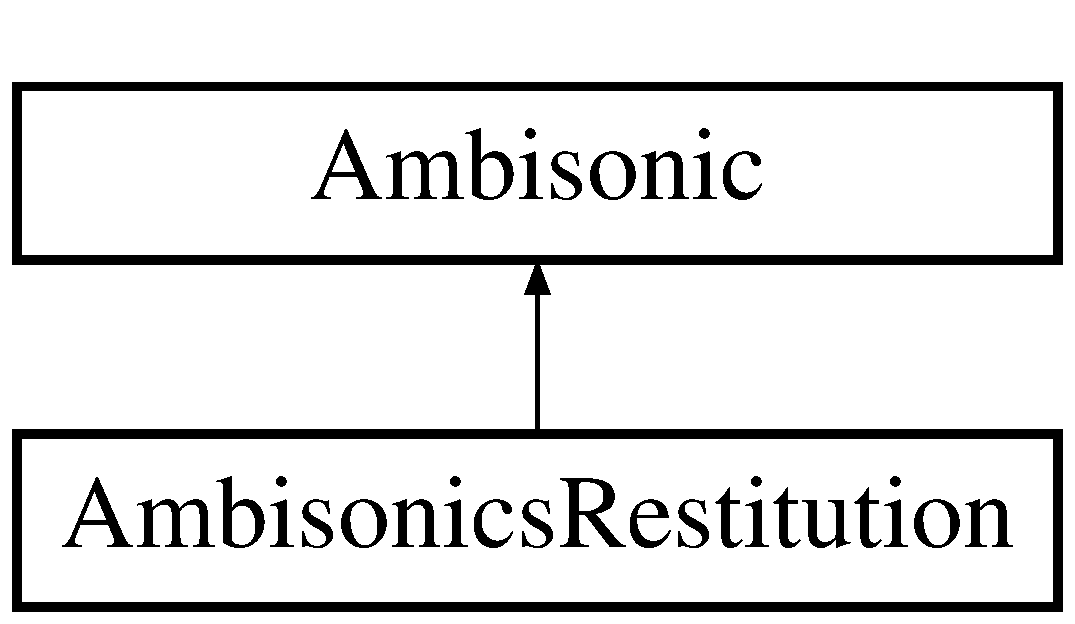
\includegraphics[height=2.000000cm]{class_ambisonics_restitution}
\end{center}
\end{figure}
\subsection*{Public Member Functions}
\begin{DoxyCompactItemize}
\item 
\hyperlink{class_ambisonics_restitution_a287ce5a5b5d247af6c11e7bd0e50a4ab}{Ambisonics\-Restitution} (long an\-Order=1, long a\-Number\-Of\-Loudspeakers=5, long a\-Resitution\-Mode=Hoa\-\_\-\-Amplitude\-\_\-\-Panning, long a\-Vector\-Size=0)
\end{DoxyCompactItemize}


\subsection{Detailed Description}


Definition at line 37 of file Ambisonics\-Restitution.\-h.



\subsection{Constructor \& Destructor Documentation}
\hypertarget{class_ambisonics_restitution_a287ce5a5b5d247af6c11e7bd0e50a4ab}{\index{Ambisonics\-Restitution@{Ambisonics\-Restitution}!Ambisonics\-Restitution@{Ambisonics\-Restitution}}
\index{Ambisonics\-Restitution@{Ambisonics\-Restitution}!AmbisonicsRestitution@{Ambisonics\-Restitution}}
\subsubsection[{Ambisonics\-Restitution}]{\setlength{\rightskip}{0pt plus 5cm}Ambisonics\-Restitution\-::\-Ambisonics\-Restitution (
\begin{DoxyParamCaption}
\item[{long}]{an\-Order = {\ttfamily 1}, }
\item[{long}]{a\-Number\-Of\-Loudspeakers = {\ttfamily 5}, }
\item[{long}]{a\-Resitution\-Mode = {\ttfamily Hoa\-\_\-Amplitude\-\_\-Panning}, }
\item[{long}]{a\-Vector\-Size = {\ttfamily 0}}
\end{DoxyParamCaption}
)}}\label{class_ambisonics_restitution_a287ce5a5b5d247af6c11e7bd0e50a4ab}
Hoa\-Library \-: A High Order Ambisonics Library Copyright (c) 2012-\/2013 Julien Colafrancesco, Pierre Guillot, Eliott Paris, C\-I\-C\-M, Universite Paris-\/8. All rights reserved.

Website \-: \href{http://www.mshparisnord.fr/hoalibrary/}{\tt http\-://www.\-mshparisnord.\-fr/hoalibrary/} Contacts \-: \href{mailto:cicm.mshparisnord@gmail.com}{\tt cicm.\-mshparisnord@gmail.\-com}

Redistribution and use in source and binary forms, with or without modification, are permitted provided that the following conditions are met\-:


\begin{DoxyItemize}
\item Redistributions may not be sold, nor may they be used in a commercial product or activity.
\item Redistributions of source code must retain the above copyright notice, this list of conditions and the following disclaimer.
\item Redistributions in binary form must reproduce the above copyright notice, this list of conditions and the following disclaimer in the documentation and/or other materials provided with the distribution.
\item Neither the name of the C\-I\-C\-M nor the names of its contributors may be used to endorse or promote products derived from this software without specific prior written permission.
\end{DoxyItemize}

T\-H\-I\-S S\-O\-F\-T\-W\-A\-R\-E I\-S P\-R\-O\-V\-I\-D\-E\-D B\-Y T\-H\-E C\-O\-P\-Y\-R\-I\-G\-H\-T H\-O\-L\-D\-E\-R\-S A\-N\-D C\-O\-N\-T\-R\-I\-B\-U\-T\-O\-R\-S \char`\"{}\-A\-S I\-S\char`\"{} A\-N\-D A\-N\-Y E\-X\-P\-R\-E\-S\-S O\-R I\-M\-P\-L\-I\-E\-D W\-A\-R\-R\-A\-N\-T\-I\-E\-S, I\-N\-C\-L\-U\-D\-I\-N\-G, B\-U\-T N\-O\-T L\-I\-M\-I\-T\-E\-D T\-O, T\-H\-E I\-M\-P\-L\-I\-E\-D W\-A\-R\-R\-A\-N\-T\-I\-E\-S O\-F M\-E\-R\-C\-H\-A\-N\-T\-A\-B\-I\-L\-I\-T\-Y A\-N\-D F\-I\-T\-N\-E\-S\-S F\-O\-R A P\-A\-R\-T\-I\-C\-U\-L\-A\-R P\-U\-R\-P\-O\-S\-E A\-R\-E D\-I\-S\-C\-L\-A\-I\-M\-E\-D. I\-N N\-O E\-V\-E\-N\-T S\-H\-A\-L\-L T\-H\-E C\-O\-P\-Y\-R\-I\-G\-H\-T H\-O\-L\-D\-E\-R O\-R C\-O\-N\-T\-R\-I\-B\-U\-T\-O\-R\-S B\-E L\-I\-A\-B\-L\-E F\-O\-R A\-N\-Y D\-I\-R\-E\-C\-T, I\-N\-D\-I\-R\-E\-C\-T, I\-N\-C\-I\-D\-E\-N\-T\-A\-L, S\-P\-E\-C\-I\-A\-L, E\-X\-E\-M\-P\-L\-A\-R\-Y, O\-R C\-O\-N\-S\-E\-Q\-U\-E\-N\-T\-I\-A\-L D\-A\-M\-A\-G\-E\-S (I\-N\-C\-L\-U\-D\-I\-N\-G, B\-U\-T N\-O\-T L\-I\-M\-I\-T\-E\-D T\-O, P\-R\-O\-C\-U\-R\-E\-M\-E\-N\-T O\-F S\-U\-B\-S\-T\-I\-T\-U\-T\-E G\-O\-O\-D\-S O\-R S\-E\-R\-V\-I\-C\-E\-S; L\-O\-S\-S O\-F U\-S\-E, D\-A\-T\-A, O\-R P\-R\-O\-F\-I\-T\-S; O\-R B\-U\-S\-I\-N\-E\-S\-S I\-N\-T\-E\-R\-R\-U\-P\-T\-I\-O\-N) H\-O\-W\-E\-V\-E\-R C\-A\-U\-S\-E\-D A\-N\-D O\-N A\-N\-Y T\-H\-E\-O\-R\-Y O\-F L\-I\-A\-B\-I\-L\-I\-T\-Y, W\-H\-E\-T\-H\-E\-R I\-N C\-O\-N\-T\-R\-A\-C\-T, S\-T\-R\-I\-C\-T L\-I\-A\-B\-I\-L\-I\-T\-Y, O\-R T\-O\-R\-T (I\-N\-C\-L\-U\-D\-I\-N\-G N\-E\-G\-L\-I\-G\-E\-N\-C\-E O\-R O\-T\-H\-E\-R\-W\-I\-S\-E) A\-R\-I\-S\-I\-N\-G I\-N A\-N\-Y W\-A\-Y O\-U\-T O\-F T\-H\-E U\-S\-E O\-F T\-H\-I\-S S\-O\-F\-T\-W\-A\-R\-E, E\-V\-E\-N I\-F A\-D\-V\-I\-S\-E\-D O\-F T\-H\-E P\-O\-S\-S\-I\-B\-I\-L\-I\-T\-Y O\-F S\-U\-C\-H D\-A\-M\-A\-G\-E. 

Definition at line 28 of file Ambisonics\-Restitution.\-cpp.



The documentation for this class was generated from the following files\-:\begin{DoxyCompactItemize}
\item 
/\-Users/elioton/\-Documents/programmation/\-C\-I\-C\-M/source\-Tree/\-Hoa\-Library/\-Sources/hoa\-Restitution/Ambisonics\-Restitution.\-h\item 
/\-Users/elioton/\-Documents/programmation/\-C\-I\-C\-M/source\-Tree/\-Hoa\-Library/\-Sources/hoa\-Restitution/Ambisonics\-Restitution.\-cpp\end{DoxyCompactItemize}

\hypertarget{class_ambisonics_ring_modulation}{\section{Ambisonics\-Ring\-Modulation Class Reference}
\label{class_ambisonics_ring_modulation}\index{Ambisonics\-Ring\-Modulation@{Ambisonics\-Ring\-Modulation}}
}


{\ttfamily \#include $<$Ambisonics\-Ring\-Modulation.\-h$>$}

Inheritance diagram for Ambisonics\-Ring\-Modulation\-:\begin{figure}[H]
\begin{center}
\leavevmode
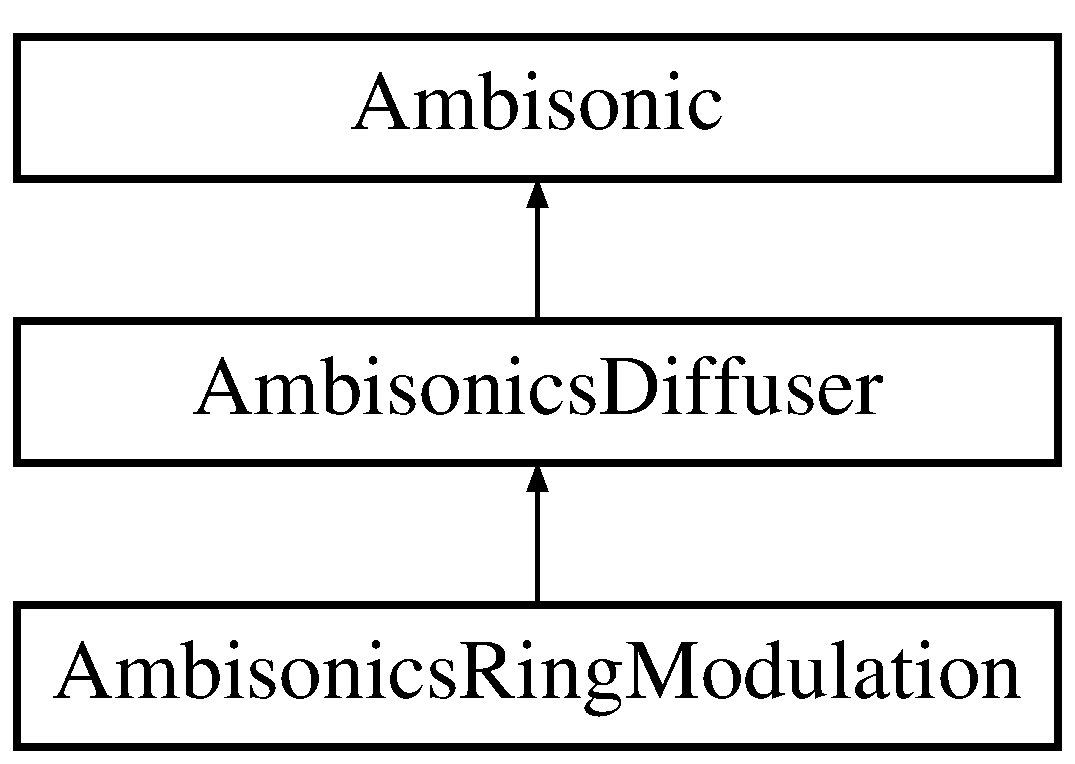
\includegraphics[height=3.000000cm]{class_ambisonics_ring_modulation}
\end{center}
\end{figure}
\subsection*{Public Member Functions}
\begin{DoxyCompactItemize}
\item 
\hyperlink{class_ambisonics_ring_modulation_aacc4d01d890203fb04536567f7299674}{Ambisonics\-Ring\-Modulation} (long an\-Order=1, bool a\-Mode=Hoa\-\_\-\-Post\-\_\-\-Encoding, long a\-Vector\-Size=0, long a\-Sampling\-Rate=44100)
\end{DoxyCompactItemize}


\subsection{Detailed Description}
Hoa\-Library \-: A High Order Ambisonics Library Copyright (c) 2012-\/2013 Julien Colafrancesco, Pierre Guillot, Eliott Paris, C\-I\-C\-M, Universite Paris-\/8. All rights reserved.

Website \-: \href{http://www.mshparisnord.fr/hoalibrary/}{\tt http\-://www.\-mshparisnord.\-fr/hoalibrary/} Contacts \-: \href{mailto:cicm.mshparisnord@gmail.com}{\tt cicm.\-mshparisnord@gmail.\-com}

Redistribution and use in source and binary forms, with or without modification, are permitted provided that the following conditions are met\-:


\begin{DoxyItemize}
\item Redistributions may not be sold, nor may they be used in a commercial product or activity.
\item Redistributions of source code must retain the above copyright notice, this list of conditions and the following disclaimer.
\item Redistributions in binary form must reproduce the above copyright notice, this list of conditions and the following disclaimer in the documentation and/or other materials provided with the distribution.
\item Neither the name of the C\-I\-C\-M nor the names of its contributors may be used to endorse or promote products derived from this software without specific prior written permission.
\end{DoxyItemize}

T\-H\-I\-S S\-O\-F\-T\-W\-A\-R\-E I\-S P\-R\-O\-V\-I\-D\-E\-D B\-Y T\-H\-E C\-O\-P\-Y\-R\-I\-G\-H\-T H\-O\-L\-D\-E\-R\-S A\-N\-D C\-O\-N\-T\-R\-I\-B\-U\-T\-O\-R\-S \char`\"{}\-A\-S I\-S\char`\"{} A\-N\-D A\-N\-Y E\-X\-P\-R\-E\-S\-S O\-R I\-M\-P\-L\-I\-E\-D W\-A\-R\-R\-A\-N\-T\-I\-E\-S, I\-N\-C\-L\-U\-D\-I\-N\-G, B\-U\-T N\-O\-T L\-I\-M\-I\-T\-E\-D T\-O, T\-H\-E I\-M\-P\-L\-I\-E\-D W\-A\-R\-R\-A\-N\-T\-I\-E\-S O\-F M\-E\-R\-C\-H\-A\-N\-T\-A\-B\-I\-L\-I\-T\-Y A\-N\-D F\-I\-T\-N\-E\-S\-S F\-O\-R A P\-A\-R\-T\-I\-C\-U\-L\-A\-R P\-U\-R\-P\-O\-S\-E A\-R\-E D\-I\-S\-C\-L\-A\-I\-M\-E\-D. I\-N N\-O E\-V\-E\-N\-T S\-H\-A\-L\-L T\-H\-E C\-O\-P\-Y\-R\-I\-G\-H\-T H\-O\-L\-D\-E\-R O\-R C\-O\-N\-T\-R\-I\-B\-U\-T\-O\-R\-S B\-E L\-I\-A\-B\-L\-E F\-O\-R A\-N\-Y D\-I\-R\-E\-C\-T, I\-N\-D\-I\-R\-E\-C\-T, I\-N\-C\-I\-D\-E\-N\-T\-A\-L, S\-P\-E\-C\-I\-A\-L, E\-X\-E\-M\-P\-L\-A\-R\-Y, O\-R C\-O\-N\-S\-E\-Q\-U\-E\-N\-T\-I\-A\-L D\-A\-M\-A\-G\-E\-S (I\-N\-C\-L\-U\-D\-I\-N\-G, B\-U\-T N\-O\-T L\-I\-M\-I\-T\-E\-D T\-O, P\-R\-O\-C\-U\-R\-E\-M\-E\-N\-T O\-F S\-U\-B\-S\-T\-I\-T\-U\-T\-E G\-O\-O\-D\-S O\-R S\-E\-R\-V\-I\-C\-E\-S; L\-O\-S\-S O\-F U\-S\-E, D\-A\-T\-A, O\-R P\-R\-O\-F\-I\-T\-S; O\-R B\-U\-S\-I\-N\-E\-S\-S I\-N\-T\-E\-R\-R\-U\-P\-T\-I\-O\-N) H\-O\-W\-E\-V\-E\-R C\-A\-U\-S\-E\-D A\-N\-D O\-N A\-N\-Y T\-H\-E\-O\-R\-Y O\-F L\-I\-A\-B\-I\-L\-I\-T\-Y, W\-H\-E\-T\-H\-E\-R I\-N C\-O\-N\-T\-R\-A\-C\-T, S\-T\-R\-I\-C\-T L\-I\-A\-B\-I\-L\-I\-T\-Y, O\-R T\-O\-R\-T (I\-N\-C\-L\-U\-D\-I\-N\-G N\-E\-G\-L\-I\-G\-E\-N\-C\-E O\-R O\-T\-H\-E\-R\-W\-I\-S\-E) A\-R\-I\-S\-I\-N\-G I\-N A\-N\-Y W\-A\-Y O\-U\-T O\-F T\-H\-E U\-S\-E O\-F T\-H\-I\-S S\-O\-F\-T\-W\-A\-R\-E, E\-V\-E\-N I\-F A\-D\-V\-I\-S\-E\-D O\-F T\-H\-E P\-O\-S\-S\-I\-B\-I\-L\-I\-T\-Y O\-F S\-U\-C\-H D\-A\-M\-A\-G\-E. 

Definition at line 31 of file Ambisonics\-Ring\-Modulation.\-h.



\subsection{Constructor \& Destructor Documentation}
\hypertarget{class_ambisonics_ring_modulation_aacc4d01d890203fb04536567f7299674}{\index{Ambisonics\-Ring\-Modulation@{Ambisonics\-Ring\-Modulation}!Ambisonics\-Ring\-Modulation@{Ambisonics\-Ring\-Modulation}}
\index{Ambisonics\-Ring\-Modulation@{Ambisonics\-Ring\-Modulation}!AmbisonicsRingModulation@{Ambisonics\-Ring\-Modulation}}
\subsubsection[{Ambisonics\-Ring\-Modulation}]{\setlength{\rightskip}{0pt plus 5cm}Ambisonics\-Ring\-Modulation\-::\-Ambisonics\-Ring\-Modulation (
\begin{DoxyParamCaption}
\item[{long}]{an\-Order = {\ttfamily 1}, }
\item[{bool}]{a\-Mode = {\ttfamily Hoa\-\_\-Post\-\_\-Encoding}, }
\item[{long}]{a\-Vector\-Size = {\ttfamily 0}, }
\item[{long}]{a\-Sampling\-Rate = {\ttfamily 44100}}
\end{DoxyParamCaption}
)}}\label{class_ambisonics_ring_modulation_aacc4d01d890203fb04536567f7299674}
Hoa\-Library \-: A High Order Ambisonics Library Copyright (c) 2012-\/2013 Julien Colafrancesco, Pierre Guillot, Eliott Paris, C\-I\-C\-M, Universite Paris-\/8. All rights reserved.

Website \-: \href{http://www.mshparisnord.fr/hoalibrary/}{\tt http\-://www.\-mshparisnord.\-fr/hoalibrary/} Contacts \-: \href{mailto:cicm.mshparisnord@gmail.com}{\tt cicm.\-mshparisnord@gmail.\-com}

Redistribution and use in source and binary forms, with or without modification, are permitted provided that the following conditions are met\-:


\begin{DoxyItemize}
\item Redistributions may not be sold, nor may they be used in a commercial product or activity.
\item Redistributions of source code must retain the above copyright notice, this list of conditions and the following disclaimer.
\item Redistributions in binary form must reproduce the above copyright notice, this list of conditions and the following disclaimer in the documentation and/or other materials provided with the distribution.
\item Neither the name of the C\-I\-C\-M nor the names of its contributors may be used to endorse or promote products derived from this software without specific prior written permission.
\end{DoxyItemize}

T\-H\-I\-S S\-O\-F\-T\-W\-A\-R\-E I\-S P\-R\-O\-V\-I\-D\-E\-D B\-Y T\-H\-E C\-O\-P\-Y\-R\-I\-G\-H\-T H\-O\-L\-D\-E\-R\-S A\-N\-D C\-O\-N\-T\-R\-I\-B\-U\-T\-O\-R\-S \char`\"{}\-A\-S I\-S\char`\"{} A\-N\-D A\-N\-Y E\-X\-P\-R\-E\-S\-S O\-R I\-M\-P\-L\-I\-E\-D W\-A\-R\-R\-A\-N\-T\-I\-E\-S, I\-N\-C\-L\-U\-D\-I\-N\-G, B\-U\-T N\-O\-T L\-I\-M\-I\-T\-E\-D T\-O, T\-H\-E I\-M\-P\-L\-I\-E\-D W\-A\-R\-R\-A\-N\-T\-I\-E\-S O\-F M\-E\-R\-C\-H\-A\-N\-T\-A\-B\-I\-L\-I\-T\-Y A\-N\-D F\-I\-T\-N\-E\-S\-S F\-O\-R A P\-A\-R\-T\-I\-C\-U\-L\-A\-R P\-U\-R\-P\-O\-S\-E A\-R\-E D\-I\-S\-C\-L\-A\-I\-M\-E\-D. I\-N N\-O E\-V\-E\-N\-T S\-H\-A\-L\-L T\-H\-E C\-O\-P\-Y\-R\-I\-G\-H\-T H\-O\-L\-D\-E\-R O\-R C\-O\-N\-T\-R\-I\-B\-U\-T\-O\-R\-S B\-E L\-I\-A\-B\-L\-E F\-O\-R A\-N\-Y D\-I\-R\-E\-C\-T, I\-N\-D\-I\-R\-E\-C\-T, I\-N\-C\-I\-D\-E\-N\-T\-A\-L, S\-P\-E\-C\-I\-A\-L, E\-X\-E\-M\-P\-L\-A\-R\-Y, O\-R C\-O\-N\-S\-E\-Q\-U\-E\-N\-T\-I\-A\-L D\-A\-M\-A\-G\-E\-S (I\-N\-C\-L\-U\-D\-I\-N\-G, B\-U\-T N\-O\-T L\-I\-M\-I\-T\-E\-D T\-O, P\-R\-O\-C\-U\-R\-E\-M\-E\-N\-T O\-F S\-U\-B\-S\-T\-I\-T\-U\-T\-E G\-O\-O\-D\-S O\-R S\-E\-R\-V\-I\-C\-E\-S; L\-O\-S\-S O\-F U\-S\-E, D\-A\-T\-A, O\-R P\-R\-O\-F\-I\-T\-S; O\-R B\-U\-S\-I\-N\-E\-S\-S I\-N\-T\-E\-R\-R\-U\-P\-T\-I\-O\-N) H\-O\-W\-E\-V\-E\-R C\-A\-U\-S\-E\-D A\-N\-D O\-N A\-N\-Y T\-H\-E\-O\-R\-Y O\-F L\-I\-A\-B\-I\-L\-I\-T\-Y, W\-H\-E\-T\-H\-E\-R I\-N C\-O\-N\-T\-R\-A\-C\-T, S\-T\-R\-I\-C\-T L\-I\-A\-B\-I\-L\-I\-T\-Y, O\-R T\-O\-R\-T (I\-N\-C\-L\-U\-D\-I\-N\-G N\-E\-G\-L\-I\-G\-E\-N\-C\-E O\-R O\-T\-H\-E\-R\-W\-I\-S\-E) A\-R\-I\-S\-I\-N\-G I\-N A\-N\-Y W\-A\-Y O\-U\-T O\-F T\-H\-E U\-S\-E O\-F T\-H\-I\-S S\-O\-F\-T\-W\-A\-R\-E, E\-V\-E\-N I\-F A\-D\-V\-I\-S\-E\-D O\-F T\-H\-E P\-O\-S\-S\-I\-B\-I\-L\-I\-T\-Y O\-F S\-U\-C\-H D\-A\-M\-A\-G\-E. 

Definition at line 28 of file Ambisonics\-Ring\-Modulation.\-cpp.



The documentation for this class was generated from the following files\-:\begin{DoxyCompactItemize}
\item 
/\-Users/\-Pierre/\-Source\-Tree/\-Hoa\-Library/\-Sources/hoa\-Ring\-Modulation/Ambisonics\-Ring\-Modulation.\-h\item 
/\-Users/\-Pierre/\-Source\-Tree/\-Hoa\-Library/\-Sources/hoa\-Ring\-Modulation/Ambisonics\-Ring\-Modulation.\-cpp\end{DoxyCompactItemize}

\hypertarget{class_ambisonics_scope}{\section{Ambisonics\-Scope Class Reference}
\label{class_ambisonics_scope}\index{Ambisonics\-Scope@{Ambisonics\-Scope}}
}


{\ttfamily \#include $<$Ambisonics\-Scope.\-h$>$}

Inheritance diagram for Ambisonics\-Scope\-:\begin{figure}[H]
\begin{center}
\leavevmode
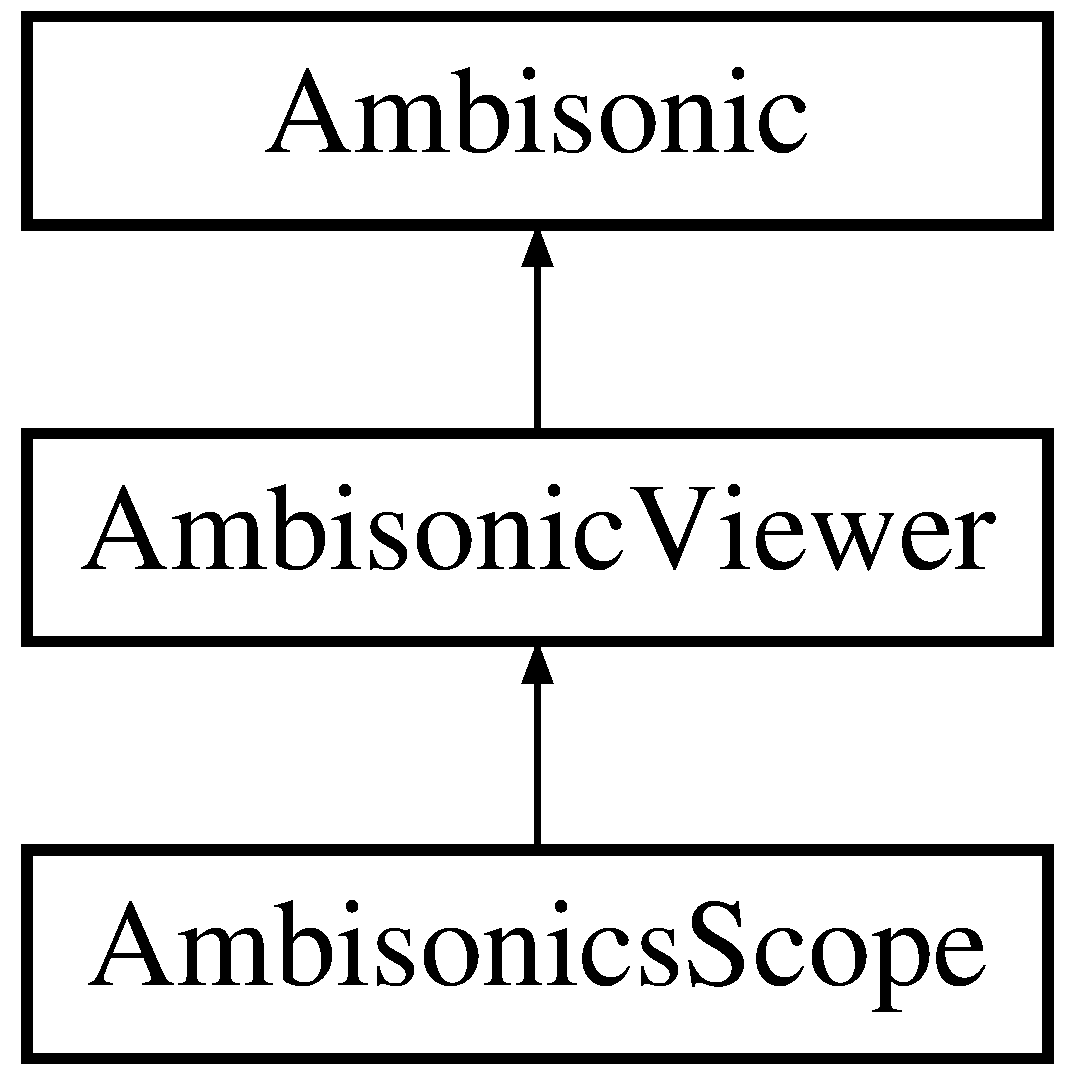
\includegraphics[height=2.000000cm]{class_ambisonics_scope}
\end{center}
\end{figure}
\subsection*{Public Member Functions}
\begin{DoxyCompactItemize}
\item 
\hyperlink{class_ambisonics_scope_a0b7854d037fb52d23898f390abc3a50c}{Ambisonics\-Scope} (long an\-Order=1, long a\-Vector\-Size=0, long a\-Sampling\-Rate=44100.)
\end{DoxyCompactItemize}


\subsection{Detailed Description}
Hoa\-Library \-: A High Order Ambisonics Library Copyright (c) 2012-\/2013 Julien Colafrancesco, Pierre Guillot, Eliott Paris, C\-I\-C\-M, Universite Paris-\/8. All rights reserved.

Website \-: \href{http://www.mshparisnord.fr/hoalibrary/}{\tt http\-://www.\-mshparisnord.\-fr/hoalibrary/} Contacts \-: \href{mailto:cicm.mshparisnord@gmail.com}{\tt cicm.\-mshparisnord@gmail.\-com}

Redistribution and use in source and binary forms, with or without modification, are permitted provided that the following conditions are met\-:


\begin{DoxyItemize}
\item Redistributions may not be sold, nor may they be used in a commercial product or activity.
\item Redistributions of source code must retain the above copyright notice, this list of conditions and the following disclaimer.
\item Redistributions in binary form must reproduce the above copyright notice, this list of conditions and the following disclaimer in the documentation and/or other materials provided with the distribution.
\item Neither the name of the C\-I\-C\-M nor the names of its contributors may be used to endorse or promote products derived from this software without specific prior written permission.
\end{DoxyItemize}

T\-H\-I\-S S\-O\-F\-T\-W\-A\-R\-E I\-S P\-R\-O\-V\-I\-D\-E\-D B\-Y T\-H\-E C\-O\-P\-Y\-R\-I\-G\-H\-T H\-O\-L\-D\-E\-R\-S A\-N\-D C\-O\-N\-T\-R\-I\-B\-U\-T\-O\-R\-S \char`\"{}\-A\-S I\-S\char`\"{} A\-N\-D A\-N\-Y E\-X\-P\-R\-E\-S\-S O\-R I\-M\-P\-L\-I\-E\-D W\-A\-R\-R\-A\-N\-T\-I\-E\-S, I\-N\-C\-L\-U\-D\-I\-N\-G, B\-U\-T N\-O\-T L\-I\-M\-I\-T\-E\-D T\-O, T\-H\-E I\-M\-P\-L\-I\-E\-D W\-A\-R\-R\-A\-N\-T\-I\-E\-S O\-F M\-E\-R\-C\-H\-A\-N\-T\-A\-B\-I\-L\-I\-T\-Y A\-N\-D F\-I\-T\-N\-E\-S\-S F\-O\-R A P\-A\-R\-T\-I\-C\-U\-L\-A\-R P\-U\-R\-P\-O\-S\-E A\-R\-E D\-I\-S\-C\-L\-A\-I\-M\-E\-D. I\-N N\-O E\-V\-E\-N\-T S\-H\-A\-L\-L T\-H\-E C\-O\-P\-Y\-R\-I\-G\-H\-T H\-O\-L\-D\-E\-R O\-R C\-O\-N\-T\-R\-I\-B\-U\-T\-O\-R\-S B\-E L\-I\-A\-B\-L\-E F\-O\-R A\-N\-Y D\-I\-R\-E\-C\-T, I\-N\-D\-I\-R\-E\-C\-T, I\-N\-C\-I\-D\-E\-N\-T\-A\-L, S\-P\-E\-C\-I\-A\-L, E\-X\-E\-M\-P\-L\-A\-R\-Y, O\-R C\-O\-N\-S\-E\-Q\-U\-E\-N\-T\-I\-A\-L D\-A\-M\-A\-G\-E\-S (I\-N\-C\-L\-U\-D\-I\-N\-G, B\-U\-T N\-O\-T L\-I\-M\-I\-T\-E\-D T\-O, P\-R\-O\-C\-U\-R\-E\-M\-E\-N\-T O\-F S\-U\-B\-S\-T\-I\-T\-U\-T\-E G\-O\-O\-D\-S O\-R S\-E\-R\-V\-I\-C\-E\-S; L\-O\-S\-S O\-F U\-S\-E, D\-A\-T\-A, O\-R P\-R\-O\-F\-I\-T\-S; O\-R B\-U\-S\-I\-N\-E\-S\-S I\-N\-T\-E\-R\-R\-U\-P\-T\-I\-O\-N) H\-O\-W\-E\-V\-E\-R C\-A\-U\-S\-E\-D A\-N\-D O\-N A\-N\-Y T\-H\-E\-O\-R\-Y O\-F L\-I\-A\-B\-I\-L\-I\-T\-Y, W\-H\-E\-T\-H\-E\-R I\-N C\-O\-N\-T\-R\-A\-C\-T, S\-T\-R\-I\-C\-T L\-I\-A\-B\-I\-L\-I\-T\-Y, O\-R T\-O\-R\-T (I\-N\-C\-L\-U\-D\-I\-N\-G N\-E\-G\-L\-I\-G\-E\-N\-C\-E O\-R O\-T\-H\-E\-R\-W\-I\-S\-E) A\-R\-I\-S\-I\-N\-G I\-N A\-N\-Y W\-A\-Y O\-U\-T O\-F T\-H\-E U\-S\-E O\-F T\-H\-I\-S S\-O\-F\-T\-W\-A\-R\-E, E\-V\-E\-N I\-F A\-D\-V\-I\-S\-E\-D O\-F T\-H\-E P\-O\-S\-S\-I\-B\-I\-L\-I\-T\-Y O\-F S\-U\-C\-H D\-A\-M\-A\-G\-E. 

Definition at line 31 of file Ambisonics\-Scope.\-h.



\subsection{Constructor \& Destructor Documentation}
\hypertarget{class_ambisonics_scope_a0b7854d037fb52d23898f390abc3a50c}{\index{Ambisonics\-Scope@{Ambisonics\-Scope}!Ambisonics\-Scope@{Ambisonics\-Scope}}
\index{Ambisonics\-Scope@{Ambisonics\-Scope}!AmbisonicsScope@{Ambisonics\-Scope}}
\subsubsection[{Ambisonics\-Scope}]{\setlength{\rightskip}{0pt plus 5cm}Ambisonics\-Scope\-::\-Ambisonics\-Scope (
\begin{DoxyParamCaption}
\item[{long}]{an\-Order = {\ttfamily 1}, }
\item[{long}]{a\-Vector\-Size = {\ttfamily 0}, }
\item[{long}]{a\-Sampling\-Rate = {\ttfamily 44100.}}
\end{DoxyParamCaption}
)}}\label{class_ambisonics_scope_a0b7854d037fb52d23898f390abc3a50c}
Hoa\-Library \-: A High Order Ambisonics Library Copyright (c) 2012-\/2013 Julien Colafrancesco, Pierre Guillot, Eliott Paris, C\-I\-C\-M, Universite Paris-\/8. All rights reserved.

Website \-: \href{http://www.mshparisnord.fr/hoalibrary/}{\tt http\-://www.\-mshparisnord.\-fr/hoalibrary/} Contacts \-: \href{mailto:cicm.mshparisnord@gmail.com}{\tt cicm.\-mshparisnord@gmail.\-com}

Redistribution and use in source and binary forms, with or without modification, are permitted provided that the following conditions are met\-:


\begin{DoxyItemize}
\item Redistributions may not be sold, nor may they be used in a commercial product or activity.
\item Redistributions of source code must retain the above copyright notice, this list of conditions and the following disclaimer.
\item Redistributions in binary form must reproduce the above copyright notice, this list of conditions and the following disclaimer in the documentation and/or other materials provided with the distribution.
\item Neither the name of the C\-I\-C\-M nor the names of its contributors may be used to endorse or promote products derived from this software without specific prior written permission.
\end{DoxyItemize}

T\-H\-I\-S S\-O\-F\-T\-W\-A\-R\-E I\-S P\-R\-O\-V\-I\-D\-E\-D B\-Y T\-H\-E C\-O\-P\-Y\-R\-I\-G\-H\-T H\-O\-L\-D\-E\-R\-S A\-N\-D C\-O\-N\-T\-R\-I\-B\-U\-T\-O\-R\-S \char`\"{}\-A\-S I\-S\char`\"{} A\-N\-D A\-N\-Y E\-X\-P\-R\-E\-S\-S O\-R I\-M\-P\-L\-I\-E\-D W\-A\-R\-R\-A\-N\-T\-I\-E\-S, I\-N\-C\-L\-U\-D\-I\-N\-G, B\-U\-T N\-O\-T L\-I\-M\-I\-T\-E\-D T\-O, T\-H\-E I\-M\-P\-L\-I\-E\-D W\-A\-R\-R\-A\-N\-T\-I\-E\-S O\-F M\-E\-R\-C\-H\-A\-N\-T\-A\-B\-I\-L\-I\-T\-Y A\-N\-D F\-I\-T\-N\-E\-S\-S F\-O\-R A P\-A\-R\-T\-I\-C\-U\-L\-A\-R P\-U\-R\-P\-O\-S\-E A\-R\-E D\-I\-S\-C\-L\-A\-I\-M\-E\-D. I\-N N\-O E\-V\-E\-N\-T S\-H\-A\-L\-L T\-H\-E C\-O\-P\-Y\-R\-I\-G\-H\-T H\-O\-L\-D\-E\-R O\-R C\-O\-N\-T\-R\-I\-B\-U\-T\-O\-R\-S B\-E L\-I\-A\-B\-L\-E F\-O\-R A\-N\-Y D\-I\-R\-E\-C\-T, I\-N\-D\-I\-R\-E\-C\-T, I\-N\-C\-I\-D\-E\-N\-T\-A\-L, S\-P\-E\-C\-I\-A\-L, E\-X\-E\-M\-P\-L\-A\-R\-Y, O\-R C\-O\-N\-S\-E\-Q\-U\-E\-N\-T\-I\-A\-L D\-A\-M\-A\-G\-E\-S (I\-N\-C\-L\-U\-D\-I\-N\-G, B\-U\-T N\-O\-T L\-I\-M\-I\-T\-E\-D T\-O, P\-R\-O\-C\-U\-R\-E\-M\-E\-N\-T O\-F S\-U\-B\-S\-T\-I\-T\-U\-T\-E G\-O\-O\-D\-S O\-R S\-E\-R\-V\-I\-C\-E\-S; L\-O\-S\-S O\-F U\-S\-E, D\-A\-T\-A, O\-R P\-R\-O\-F\-I\-T\-S; O\-R B\-U\-S\-I\-N\-E\-S\-S I\-N\-T\-E\-R\-R\-U\-P\-T\-I\-O\-N) H\-O\-W\-E\-V\-E\-R C\-A\-U\-S\-E\-D A\-N\-D O\-N A\-N\-Y T\-H\-E\-O\-R\-Y O\-F L\-I\-A\-B\-I\-L\-I\-T\-Y, W\-H\-E\-T\-H\-E\-R I\-N C\-O\-N\-T\-R\-A\-C\-T, S\-T\-R\-I\-C\-T L\-I\-A\-B\-I\-L\-I\-T\-Y, O\-R T\-O\-R\-T (I\-N\-C\-L\-U\-D\-I\-N\-G N\-E\-G\-L\-I\-G\-E\-N\-C\-E O\-R O\-T\-H\-E\-R\-W\-I\-S\-E) A\-R\-I\-S\-I\-N\-G I\-N A\-N\-Y W\-A\-Y O\-U\-T O\-F T\-H\-E U\-S\-E O\-F T\-H\-I\-S S\-O\-F\-T\-W\-A\-R\-E, E\-V\-E\-N I\-F A\-D\-V\-I\-S\-E\-D O\-F T\-H\-E P\-O\-S\-S\-I\-B\-I\-L\-I\-T\-Y O\-F S\-U\-C\-H D\-A\-M\-A\-G\-E. 

Definition at line 28 of file Ambisonics\-Scope.\-cpp.



The documentation for this class was generated from the following files\-:\begin{DoxyCompactItemize}
\item 
/\-Users/\-Pierre/\-Source\-Tree/\-Hoa\-Library/\-Sources/hoa\-Scope/Ambisonics\-Scope.\-h\item 
/\-Users/\-Pierre/\-Source\-Tree/\-Hoa\-Library/\-Sources/hoa\-Scope/Ambisonics\-Scope.\-cpp\end{DoxyCompactItemize}

\hypertarget{class_ambisonic_vector}{\section{Ambisonic\-Vector Class Reference}
\label{class_ambisonic_vector}\index{Ambisonic\-Vector@{Ambisonic\-Vector}}
}


{\ttfamily \#include $<$Ambisonic\-Vector.\-h$>$}

Inheritance diagram for Ambisonic\-Vector\-:\begin{figure}[H]
\begin{center}
\leavevmode
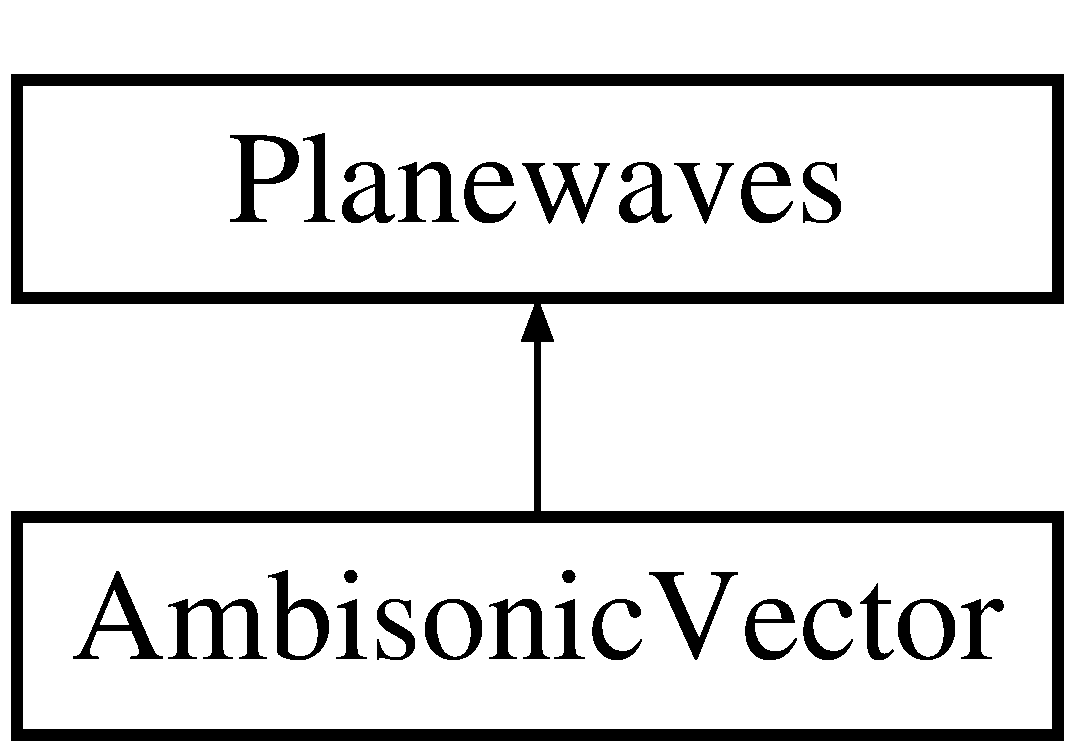
\includegraphics[height=2.000000cm]{class_ambisonic_vector}
\end{center}
\end{figure}
\subsection*{Public Member Functions}
\begin{DoxyCompactItemize}
\item 
\hyperlink{class_ambisonic_vector_ae4c02b111015ca551b50676e9989e5e1}{Ambisonic\-Vector} (long a\-Number\-Of\-Loudspeakers=1., long a\-Vector\-Size=0)
\end{DoxyCompactItemize}


\subsection{Detailed Description}
\hyperlink{interface_hoa_library}{Hoa\-Library} \-: A High Order Ambisonics Library Copyright (c) 2012-\/2013 Julien Colafrancesco, Pierre Guillot, Eliott Paris, C\-I\-C\-M, Universite Paris-\/8. All rights reserved.\-re Guillot, C\-I\-C\-M -\/ Université Paris 8 All rights reserved.

Website \-: \href{http://www.mshparisnord.fr/HoaLibrary/}{\tt http\-://www.\-mshparisnord.\-fr/\-Hoa\-Library/} Contacts \-: \href{mailto:cicm.mshparisnord@gmail.com}{\tt cicm.\-mshparisnord@gmail.\-com}

This file is part of H\-O\-A L\-I\-B\-R\-A\-R\-Y.

H\-O\-A L\-I\-B\-R\-A\-R\-Y is free software\-: you can redistribute it and/or modify it under the terms of the G\-N\-U General Public License as published by the Free Software Foundation, either version 3 of the License, or (at your option) any later version.

This program is distributed in the hope that it will be useful, but W\-I\-T\-H\-O\-U\-T A\-N\-Y W\-A\-R\-R\-A\-N\-T\-Y; without even the implied warranty of M\-E\-R\-C\-H\-A\-N\-T\-A\-B\-I\-L\-I\-T\-Y or F\-I\-T\-N\-E\-S\-S F\-O\-R A P\-A\-R\-T\-I\-C\-U\-L\-A\-R P\-U\-R\-P\-O\-S\-E. See the G\-N\-U General Public License for more details.

You should have received a copy of the G\-N\-U General Public License along with this program. If not, see \href{http://www.gnu.org/licenses/}{\tt http\-://www.\-gnu.\-org/licenses/}. 

Definition at line 32 of file Ambisonic\-Vector.\-h.



\subsection{Constructor \& Destructor Documentation}
\hypertarget{class_ambisonic_vector_ae4c02b111015ca551b50676e9989e5e1}{\index{Ambisonic\-Vector@{Ambisonic\-Vector}!Ambisonic\-Vector@{Ambisonic\-Vector}}
\index{Ambisonic\-Vector@{Ambisonic\-Vector}!AmbisonicVector@{Ambisonic\-Vector}}
\subsubsection[{Ambisonic\-Vector}]{\setlength{\rightskip}{0pt plus 5cm}Ambisonic\-Vector\-::\-Ambisonic\-Vector (
\begin{DoxyParamCaption}
\item[{long}]{a\-Number\-Of\-Loudspeakers = {\ttfamily 1.}, }
\item[{long}]{a\-Vector\-Size = {\ttfamily 0}}
\end{DoxyParamCaption}
)}}\label{class_ambisonic_vector_ae4c02b111015ca551b50676e9989e5e1}
\hyperlink{interface_hoa_library}{Hoa\-Library} \-: A High Order Ambisonics Library Copyright (c) 2012-\/2013 Julien Colafrancesco, Pierre Guillot, Eliott Paris, C\-I\-C\-M, Universite Paris-\/8. All rights reserved.\-re Guillot, C\-I\-C\-M -\/ Université Paris 8 All rights reserved.

Website \-: \href{http://www.mshparisnord.fr/HoaLibrary/}{\tt http\-://www.\-mshparisnord.\-fr/\-Hoa\-Library/} Contacts \-: \href{mailto:cicm.mshparisnord@gmail.com}{\tt cicm.\-mshparisnord@gmail.\-com}

This file is part of H\-O\-A L\-I\-B\-R\-A\-R\-Y.

H\-O\-A L\-I\-B\-R\-A\-R\-Y is free software\-: you can redistribute it and/or modify it under the terms of the G\-N\-U General Public License as published by the Free Software Foundation, either version 3 of the License, or (at your option) any later version.

This program is distributed in the hope that it will be useful, but W\-I\-T\-H\-O\-U\-T A\-N\-Y W\-A\-R\-R\-A\-N\-T\-Y; without even the implied warranty of M\-E\-R\-C\-H\-A\-N\-T\-A\-B\-I\-L\-I\-T\-Y or F\-I\-T\-N\-E\-S\-S F\-O\-R A P\-A\-R\-T\-I\-C\-U\-L\-A\-R P\-U\-R\-P\-O\-S\-E. See the G\-N\-U General Public License for more details.

You should have received a copy of the G\-N\-U General Public License along with this program. If not, see \href{http://www.gnu.org/licenses/}{\tt http\-://www.\-gnu.\-org/licenses/}. 

Definition at line 29 of file Ambisonic\-Vector.\-cpp.



The documentation for this class was generated from the following files\-:\begin{DoxyCompactItemize}
\item 
/\-Users/elioton/\-Documents/programmation/\-C\-I\-C\-M/source\-Tree/\-Hoa\-Library/\-Sources/hoa\-Vector/Ambisonic\-Vector.\-h\item 
/\-Users/elioton/\-Documents/programmation/\-C\-I\-C\-M/source\-Tree/\-Hoa\-Library/\-Sources/hoa\-Vector/Ambisonic\-Vector.\-cpp\end{DoxyCompactItemize}

\hypertarget{class_ambisonic_viewer}{\section{Ambisonic\-Viewer Class Reference}
\label{class_ambisonic_viewer}\index{Ambisonic\-Viewer@{Ambisonic\-Viewer}}
}


{\ttfamily \#include $<$Ambisonic\-Viewer.\-h$>$}

Inheritance diagram for Ambisonic\-Viewer\-:\begin{figure}[H]
\begin{center}
\leavevmode
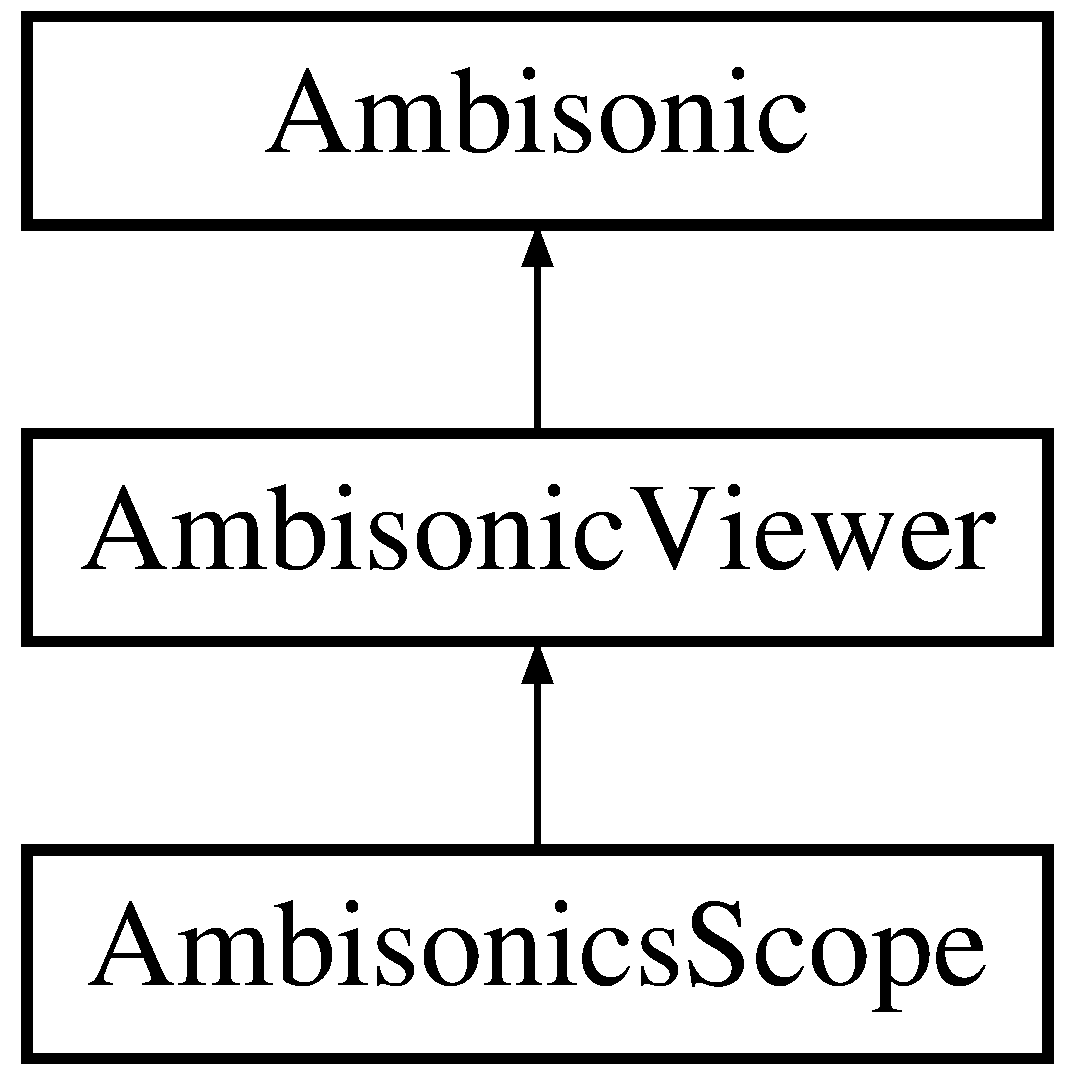
\includegraphics[height=3.000000cm]{class_ambisonic_viewer}
\end{center}
\end{figure}
\subsection*{Public Member Functions}
\begin{DoxyCompactItemize}
\item 
\hyperlink{class_ambisonic_viewer_aed38fd89c057c2b707a2bc5e91b17861}{Ambisonic\-Viewer} (long an\-Order, long a\-Vector\-Size=2, long a\-Sampling\-Rate=44100)
\end{DoxyCompactItemize}


\subsection{Detailed Description}
\hyperlink{interface_hoa_library}{Hoa\-Library} \-: A High Order Ambisonics Library Copyright (c) 2012-\/2013 Julien Colafrancesco, Pierre Guillot, Eliott Paris, C\-I\-C\-M, Universite Paris-\/8. All rights reserved.\-re Guillot, C\-I\-C\-M -\/ Université Paris 8 All rights reserved.

Website \-: \href{http://www.mshparisnord.fr/HoaLibrary/}{\tt http\-://www.\-mshparisnord.\-fr/\-Hoa\-Library/} Contacts \-: \href{mailto:cicm.mshparisnord@gmail.com}{\tt cicm.\-mshparisnord@gmail.\-com}

This file is part of H\-O\-A L\-I\-B\-R\-A\-R\-Y.

H\-O\-A L\-I\-B\-R\-A\-R\-Y is free software\-: you can redistribute it and/or modify it under the terms of the G\-N\-U General Public License as published by the Free Software Foundation, either version 3 of the License, or (at your option) any later version.

This program is distributed in the hope that it will be useful, but W\-I\-T\-H\-O\-U\-T A\-N\-Y W\-A\-R\-R\-A\-N\-T\-Y; without even the implied warranty of M\-E\-R\-C\-H\-A\-N\-T\-A\-B\-I\-L\-I\-T\-Y or F\-I\-T\-N\-E\-S\-S F\-O\-R A P\-A\-R\-T\-I\-C\-U\-L\-A\-R P\-U\-R\-P\-O\-S\-E. See the G\-N\-U General Public License for more details.

You should have received a copy of the G\-N\-U General Public License along with this program. If not, see \href{http://www.gnu.org/licenses/}{\tt http\-://www.\-gnu.\-org/licenses/}. 

Definition at line 32 of file Ambisonic\-Viewer.\-h.



\subsection{Constructor \& Destructor Documentation}
\hypertarget{class_ambisonic_viewer_aed38fd89c057c2b707a2bc5e91b17861}{\index{Ambisonic\-Viewer@{Ambisonic\-Viewer}!Ambisonic\-Viewer@{Ambisonic\-Viewer}}
\index{Ambisonic\-Viewer@{Ambisonic\-Viewer}!AmbisonicViewer@{Ambisonic\-Viewer}}
\subsubsection[{Ambisonic\-Viewer}]{\setlength{\rightskip}{0pt plus 5cm}Ambisonic\-Viewer\-::\-Ambisonic\-Viewer (
\begin{DoxyParamCaption}
\item[{long}]{an\-Order, }
\item[{long}]{a\-Vector\-Size = {\ttfamily 2}, }
\item[{long}]{a\-Sampling\-Rate = {\ttfamily 44100}}
\end{DoxyParamCaption}
)}}\label{class_ambisonic_viewer_aed38fd89c057c2b707a2bc5e91b17861}
\hyperlink{interface_hoa_library}{Hoa\-Library} \-: A High Order Ambisonics Library Copyright (c) 2012-\/2013 Julien Colafrancesco, Pierre Guillot, Eliott Paris, C\-I\-C\-M, Universite Paris-\/8. All rights reserved.\-re Guillot, C\-I\-C\-M -\/ Université Paris 8 All rights reserved.

Website \-: \href{http://www.mshparisnord.fr/HoaLibrary/}{\tt http\-://www.\-mshparisnord.\-fr/\-Hoa\-Library/} Contacts \-: \href{mailto:cicm.mshparisnord@gmail.com}{\tt cicm.\-mshparisnord@gmail.\-com}

This file is part of H\-O\-A L\-I\-B\-R\-A\-R\-Y.

H\-O\-A L\-I\-B\-R\-A\-R\-Y is free software\-: you can redistribute it and/or modify it under the terms of the G\-N\-U General Public License as published by the Free Software Foundation, either version 3 of the License, or (at your option) any later version.

This program is distributed in the hope that it will be useful, but W\-I\-T\-H\-O\-U\-T A\-N\-Y W\-A\-R\-R\-A\-N\-T\-Y; without even the implied warranty of M\-E\-R\-C\-H\-A\-N\-T\-A\-B\-I\-L\-I\-T\-Y or F\-I\-T\-N\-E\-S\-S F\-O\-R A P\-A\-R\-T\-I\-C\-U\-L\-A\-R P\-U\-R\-P\-O\-S\-E. See the G\-N\-U General Public License for more details.

You should have received a copy of the G\-N\-U General Public License along with this program. If not, see \href{http://www.gnu.org/licenses/}{\tt http\-://www.\-gnu.\-org/licenses/}. 

Definition at line 29 of file Ambisonic\-Viewer.\-cpp.



The documentation for this class was generated from the following files\-:\begin{DoxyCompactItemize}
\item 
/\-Users/elioton/\-Documents/programmation/\-C\-I\-C\-M/source\-Tree/\-Hoa\-Library/\-Sources/hoa\-Ambisonics/Ambisonic\-Viewer.\-h\item 
/\-Users/elioton/\-Documents/programmation/\-C\-I\-C\-M/source\-Tree/\-Hoa\-Library/\-Sources/hoa\-Ambisonics/Ambisonic\-Viewer.\-cpp\end{DoxyCompactItemize}

\hypertarget{class_ambisonic_virtual_mic_u_i}{\section{Ambisonic\-Virtual\-Mic\-U\-I Class Reference}
\label{class_ambisonic_virtual_mic_u_i}\index{Ambisonic\-Virtual\-Mic\-U\-I@{Ambisonic\-Virtual\-Mic\-U\-I}}
}


The documentation for this class was generated from the following files\-:\begin{DoxyCompactItemize}
\item 
/\-Users/\-Pierre/\-Source\-Tree/\-Hoa\-Library/\-Sources/hoa\-Recomposer/Ambisonic\-Virtual\-Mic\-U\-I.\-h\item 
/\-Users/\-Pierre/\-Source\-Tree/\-Hoa\-Library/\-Sources/hoa\-Recomposer/Ambisonic\-Virtual\-Mic\-U\-I.\-cpp\end{DoxyCompactItemize}

\hypertarget{class_ambisonic_virtual_mic_u_i_manager}{\section{Ambisonic\-Virtual\-Mic\-U\-I\-Manager Class Reference}
\label{class_ambisonic_virtual_mic_u_i_manager}\index{Ambisonic\-Virtual\-Mic\-U\-I\-Manager@{Ambisonic\-Virtual\-Mic\-U\-I\-Manager}}
}


\subsection{Detailed Description}


Definition at line 32 of file Ambisonic\-Virtual\-Mic\-U\-I\-Manager.\-h.



The documentation for this class was generated from the following files\-:\begin{DoxyCompactItemize}
\item 
/\-Users/\-Pierre/\-Source\-Tree/\-Hoa\-Library/\-Sources/hoa\-Recomposer/Ambisonic\-Virtual\-Mic\-U\-I\-Manager.\-h\item 
/\-Users/\-Pierre/\-Source\-Tree/\-Hoa\-Library/\-Sources/hoa\-Recomposer/Ambisonic\-Virtual\-Mic\-U\-I\-Manager.\-cpp\end{DoxyCompactItemize}

\hypertarget{class_ambisonic_wider}{\section{Ambisonic\-Wider Class Reference}
\label{class_ambisonic_wider}\index{Ambisonic\-Wider@{Ambisonic\-Wider}}
}


An ambisonic wider.  




{\ttfamily \#include $<$Ambisonic\-Wider.\-h$>$}

Inheritance diagram for Ambisonic\-Wider\-:\begin{figure}[H]
\begin{center}
\leavevmode
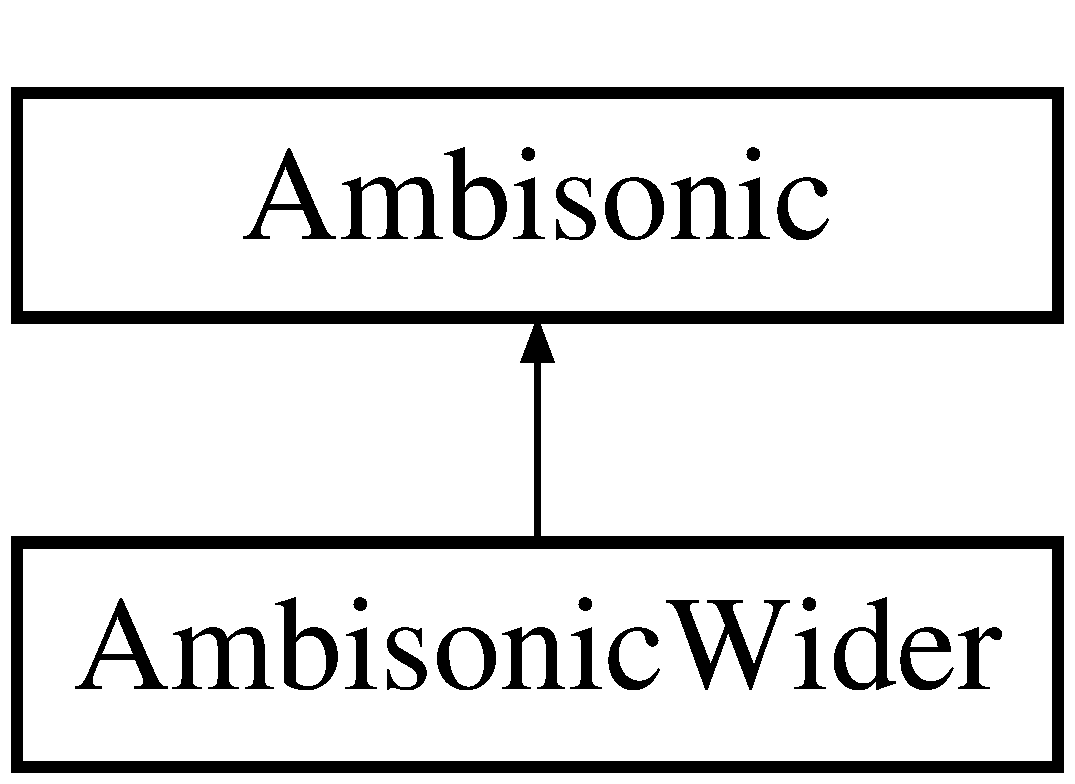
\includegraphics[height=2.000000cm]{class_ambisonic_wider}
\end{center}
\end{figure}
\subsection*{Public Member Functions}
\begin{DoxyCompactItemize}
\item 
\hyperlink{class_ambisonic_wider_a8e46f8e6bc4eda1c6c17f632d2e1a12f}{Ambisonic\-Wider} (long an\-Order=1, long a\-Vector\-Size=2)
\begin{DoxyCompactList}\small\item\em The wider constructor. \end{DoxyCompactList}\item 
void \hyperlink{class_ambisonic_wider_a26597b62bcb8d892591ad5362702edca}{set\-Widen\-Value} (double a\-Widening\-Value)
\begin{DoxyCompactList}\small\item\em Set the widening value. \end{DoxyCompactList}\item 
void \hyperlink{class_ambisonic_wider_af970c4c71f96afa96649d9c1a1387043}{set\-Vector\-Size} (long a\-Vector\-Size)
\begin{DoxyCompactList}\small\item\em Set the size of the samples block. \end{DoxyCompactList}\item 
std\-::string \hyperlink{class_ambisonic_wider_a405f99a0427aa56d945acbe7f1a09582}{get\-Input\-Name} (long an\-Index)
\begin{DoxyCompactList}\small\item\em Retreive the name of an input. \end{DoxyCompactList}\item 
std\-::string \hyperlink{class_ambisonic_wider_a5c5c88a09477812991122b290117faf9}{get\-Output\-Name} (long an\-Index)
\begin{DoxyCompactList}\small\item\em Retreive the name of an output. \end{DoxyCompactList}\item 
\hypertarget{class_ambisonic_wider_a98b370684ad2cc2d1bdf75add135f1c7}{\hyperlink{class_ambisonic_wider_a98b370684ad2cc2d1bdf75add135f1c7}{$\sim$\-Ambisonic\-Wider} ()}\label{class_ambisonic_wider_a98b370684ad2cc2d1bdf75add135f1c7}

\begin{DoxyCompactList}\small\item\em The wider destructor. \end{DoxyCompactList}\end{DoxyCompactItemize}
\subsection*{Additional Inherited Members}


\subsection{Detailed Description}
An ambisonic wider. 

The wider class can be used to wide the diffusion of a localised sound. The order depending signals are weighted and appear in a logarithmic way to have linear changes. The class processing functions \-:sample by sample -\/ in place. sample by sample -\/ in place -\/ widening value setter. sample by sample -\/ not in place. sample by sample -\/ not in place -\/ widening value setter. samples block -\/ in place. samples block -\/ in place -\/ widening value setter. samples block -\/ not in place. samples block -\/ not in place -\/ widening value setter. 

\subsection{Constructor \& Destructor Documentation}
\hypertarget{class_ambisonic_wider_a8e46f8e6bc4eda1c6c17f632d2e1a12f}{\index{Ambisonic\-Wider@{Ambisonic\-Wider}!Ambisonic\-Wider@{Ambisonic\-Wider}}
\index{Ambisonic\-Wider@{Ambisonic\-Wider}!AmbisonicWider@{Ambisonic\-Wider}}
\subsubsection[{Ambisonic\-Wider}]{\setlength{\rightskip}{0pt plus 5cm}Ambisonic\-Wider\-::\-Ambisonic\-Wider (
\begin{DoxyParamCaption}
\item[{long}]{an\-Order = {\ttfamily 1}, }
\item[{long}]{a\-Vector\-Size = {\ttfamily 2}}
\end{DoxyParamCaption}
)}}\label{class_ambisonic_wider_a8e46f8e6bc4eda1c6c17f632d2e1a12f}


The wider constructor. 


\begin{DoxyParams}{Parameters}
{\em an\-Order} & The ambisonic decomposition order. \\
\hline
{\em a\-Vector\-Size} & The size of the samples block.\\
\hline
\end{DoxyParams}
\hyperlink{interface_hoa_library}{Hoa\-Library} \-: A High Order Ambisonics Library Copyright (c) 2012-\/2013 Julien Colafrancesco, Pierre Guillot, Eliott Paris, C\-I\-C\-M, Universite Paris-\/8. All rights reserved.\-re Guillot, C\-I\-C\-M -\/ Université Paris 8 All rights reserved.

Website \-: \href{http://www.mshparisnord.fr/HoaLibrary/}{\tt http\-://www.\-mshparisnord.\-fr/\-Hoa\-Library/} Contacts \-: \href{mailto:cicm.mshparisnord@gmail.com}{\tt cicm.\-mshparisnord@gmail.\-com}

This file is part of H\-O\-A L\-I\-B\-R\-A\-R\-Y.

H\-O\-A L\-I\-B\-R\-A\-R\-Y is free software\-: you can redistribute it and/or modify it under the terms of the G\-N\-U General Public License as published by the Free Software Foundation, either version 3 of the License, or (at your option) any later version.

This program is distributed in the hope that it will be useful, but W\-I\-T\-H\-O\-U\-T A\-N\-Y W\-A\-R\-R\-A\-N\-T\-Y; without even the implied warranty of M\-E\-R\-C\-H\-A\-N\-T\-A\-B\-I\-L\-I\-T\-Y or F\-I\-T\-N\-E\-S\-S F\-O\-R A P\-A\-R\-T\-I\-C\-U\-L\-A\-R P\-U\-R\-P\-O\-S\-E. See the G\-N\-U General Public License for more details.

You should have received a copy of the G\-N\-U General Public License along with this program. If not, see \href{http://www.gnu.org/licenses/}{\tt http\-://www.\-gnu.\-org/licenses/}. 

\subsection{Member Function Documentation}
\hypertarget{class_ambisonic_wider_a405f99a0427aa56d945acbe7f1a09582}{\index{Ambisonic\-Wider@{Ambisonic\-Wider}!get\-Input\-Name@{get\-Input\-Name}}
\index{get\-Input\-Name@{get\-Input\-Name}!AmbisonicWider@{Ambisonic\-Wider}}
\subsubsection[{get\-Input\-Name}]{\setlength{\rightskip}{0pt plus 5cm}std\-::string Ambisonic\-Wider\-::get\-Input\-Name (
\begin{DoxyParamCaption}
\item[{long}]{an\-Index}
\end{DoxyParamCaption}
)}}\label{class_ambisonic_wider_a405f99a0427aa56d945acbe7f1a09582}


Retreive the name of an input. 


\begin{DoxyParams}{Parameters}
{\em an\-Index} & The input index. \\
\hline
\end{DoxyParams}
\hypertarget{class_ambisonic_wider_a5c5c88a09477812991122b290117faf9}{\index{Ambisonic\-Wider@{Ambisonic\-Wider}!get\-Output\-Name@{get\-Output\-Name}}
\index{get\-Output\-Name@{get\-Output\-Name}!AmbisonicWider@{Ambisonic\-Wider}}
\subsubsection[{get\-Output\-Name}]{\setlength{\rightskip}{0pt plus 5cm}std\-::string Ambisonic\-Wider\-::get\-Output\-Name (
\begin{DoxyParamCaption}
\item[{long}]{an\-Index}
\end{DoxyParamCaption}
)}}\label{class_ambisonic_wider_a5c5c88a09477812991122b290117faf9}


Retreive the name of an output. 


\begin{DoxyParams}{Parameters}
{\em an\-Index} & The outpout index. \\
\hline
\end{DoxyParams}
\hypertarget{class_ambisonic_wider_af970c4c71f96afa96649d9c1a1387043}{\index{Ambisonic\-Wider@{Ambisonic\-Wider}!set\-Vector\-Size@{set\-Vector\-Size}}
\index{set\-Vector\-Size@{set\-Vector\-Size}!AmbisonicWider@{Ambisonic\-Wider}}
\subsubsection[{set\-Vector\-Size}]{\setlength{\rightskip}{0pt plus 5cm}void Ambisonic\-Wider\-::set\-Vector\-Size (
\begin{DoxyParamCaption}
\item[{long}]{a\-Vector\-Size}
\end{DoxyParamCaption}
)}}\label{class_ambisonic_wider_af970c4c71f96afa96649d9c1a1387043}


Set the size of the samples block. 


\begin{DoxyParams}{Parameters}
{\em a\-Vector\-Size} & The size of the samples block (must be a power of 2). \\
\hline
\end{DoxyParams}
\hypertarget{class_ambisonic_wider_a26597b62bcb8d892591ad5362702edca}{\index{Ambisonic\-Wider@{Ambisonic\-Wider}!set\-Widen\-Value@{set\-Widen\-Value}}
\index{set\-Widen\-Value@{set\-Widen\-Value}!AmbisonicWider@{Ambisonic\-Wider}}
\subsubsection[{set\-Widen\-Value}]{\setlength{\rightskip}{0pt plus 5cm}void Ambisonic\-Wider\-::set\-Widen\-Value (
\begin{DoxyParamCaption}
\item[{double}]{a\-Widening\-Value}
\end{DoxyParamCaption}
)}}\label{class_ambisonic_wider_a26597b62bcb8d892591ad5362702edca}


Set the widening value. 


\begin{DoxyParams}{Parameters}
{\em a\-Widening\-Value} & The widening value (between 0 and 1). \\
\hline
\end{DoxyParams}


The documentation for this class was generated from the following files\-:\begin{DoxyCompactItemize}
\item 
/\-Users/\-Pierre/\-Source\-Tree/\-Hoa\-Library/\-Sources/hoa\-Wider/Ambisonic\-Wider.\-h\item 
/\-Users/\-Pierre/\-Source\-Tree/\-Hoa\-Library/\-Sources/hoa\-Wider/Ambisonic\-Wider.\-cpp\end{DoxyCompactItemize}

\hypertarget{class_boid}{\section{Boid Class Reference}
\label{class_boid}\index{Boid@{Boid}}
}


\subsection{Detailed Description}


Definition at line 74 of file Boids\-Manager.\-h.



The documentation for this class was generated from the following file\-:\begin{DoxyCompactItemize}
\item 
/\-Users/elioton/\-Documents/programmation/\-C\-I\-C\-M/source\-Tree/\-Hoa\-Library/\-Sources/hoa\-Boids/Boids\-Manager.\-h\end{DoxyCompactItemize}

\hypertarget{class_boids_manager}{\section{Boids\-Manager Class Reference}
\label{class_boids_manager}\index{Boids\-Manager@{Boids\-Manager}}
}
\subsection*{Public Member Functions}
\begin{DoxyCompactItemize}
\item 
\hyperlink{class_boids_manager_aa0e85ff06c7c9912b3f22673fb99d837}{Boids\-Manager} ()
\item 
\hypertarget{class_boids_manager_a17be98b043bf439bfb10a9f300308e35}{void {\bfseries init\-Flock} ()}\label{class_boids_manager_a17be98b043bf439bfb10a9f300308e35}

\item 
\hypertarget{class_boids_manager_a6f4b1b6a060c865b4188b643cc66d284}{void {\bfseries reset\-Boids} ()}\label{class_boids_manager_a6f4b1b6a060c865b4188b643cc66d284}

\item 
\hypertarget{class_boids_manager_a16183cc1c98ffc366649a3ce477d298f}{void {\bfseries update} ()}\label{class_boids_manager_a16183cc1c98ffc366649a3ce477d298f}

\item 
\hypertarget{class_boids_manager_a69f0d046aeeb6db1679a040e4e913008}{\hyperlink{struct_point2d}{Point2d} {\bfseries Find\-Flock\-Center} ()}\label{class_boids_manager_a69f0d046aeeb6db1679a040e4e913008}

\item 
\hypertarget{class_boids_manager_af272d7d0716735458776acf48b78222e}{float {\bfseries Match\-And\-Avoid\-Neighbors} (short the\-Boid, \hyperlink{struct_velocity}{Velocity} $\ast$match\-Neighbor\-Vel, \hyperlink{struct_velocity}{Velocity} $\ast$avoid\-Neighbor\-Vel)}\label{class_boids_manager_af272d7d0716735458776acf48b78222e}

\item 
\hypertarget{class_boids_manager_accb5827c74c27972be0a1b4560bb6a3f}{\hyperlink{struct_velocity}{Velocity} {\bfseries Seek\-Point} (short the\-Boid, \hyperlink{struct_point2d}{Point2d} seek\-Pt)}\label{class_boids_manager_accb5827c74c27972be0a1b4560bb6a3f}

\item 
\hypertarget{class_boids_manager_a91f17d1297bcf1322fe57b6928b866b0}{\hyperlink{struct_velocity}{Velocity} {\bfseries Avoid\-Walls} (short the\-Boid)}\label{class_boids_manager_a91f17d1297bcf1322fe57b6928b866b0}

\item 
\hypertarget{class_boids_manager_af66fa1589341596a77dbd6f7e13023a7}{double {\bfseries Dist\-Sqr\-To\-Pt} (\hyperlink{struct_point2d}{Point2d} first\-Point, \hyperlink{struct_point2d}{Point2d} second\-Point)}\label{class_boids_manager_af66fa1589341596a77dbd6f7e13023a7}

\item 
\hypertarget{class_boids_manager_a188dcc3a8e53700815838d0ff5a2cff4}{void {\bfseries Normalize\-Velocity} (\hyperlink{struct_velocity}{Velocity} $\ast$direction)}\label{class_boids_manager_a188dcc3a8e53700815838d0ff5a2cff4}

\item 
\hypertarget{class_boids_manager_a2b41e006b4edf55b10bc5854a7364b58}{bool {\bfseries In\-Front} (\hyperlink{class_boid}{Boid} $\ast$the\-Boid, \hyperlink{class_boid}{Boid} $\ast$neighbor)}\label{class_boids_manager_a2b41e006b4edf55b10bc5854a7364b58}

\item 
\hypertarget{class_boids_manager_a08722665999e7476f58ed5e300f4af32}{void {\bfseries boid\-\_\-set\-\_\-pos} (long index, double pos\-X, double pos\-Y)}\label{class_boids_manager_a08722665999e7476f58ed5e300f4af32}

\item 
\hypertarget{class_boids_manager_a5f3baec1959a0e0de26bddab21710312}{void {\bfseries boid\-\_\-set\-\_\-dir} (long index, double dir\-X, double dir\-Y)}\label{class_boids_manager_a5f3baec1959a0e0de26bddab21710312}

\item 
\hypertarget{class_boids_manager_a60b68a6d745989e2eedaf567c0605d0a}{void {\bfseries boid\-\_\-set\-\_\-speed} (long index, double speed)}\label{class_boids_manager_a60b68a6d745989e2eedaf567c0605d0a}

\item 
\hypertarget{class_boids_manager_ad30fc5fde2c8cc54e20396b7fe1458ce}{void {\bfseries boid\-\_\-set\-\_\-speedinv} (long index)}\label{class_boids_manager_ad30fc5fde2c8cc54e20396b7fe1458ce}

\item 
\hypertarget{class_boids_manager_a6850560000b33739e9861ed881c10886}{void {\bfseries set\-Number\-Of\-Boids} (long \-\_\-number\-Of\-Boids)}\label{class_boids_manager_a6850560000b33739e9861ed881c10886}

\item 
\hypertarget{class_boids_manager_a77d11b4a7a9fe6d3115861c4719a0a91}{void {\bfseries set\-Number\-Of\-Neighbors} (long \-\_\-number\-Of\-Neighbors)}\label{class_boids_manager_a77d11b4a7a9fe6d3115861c4719a0a91}

\item 
\hypertarget{class_boids_manager_aad30bca3303baa5d7767b980541b0f90}{void {\bfseries set\-Fly\-Rect} (double left, double right, double top, double bottom)}\label{class_boids_manager_aad30bca3303baa5d7767b980541b0f90}

\item 
\hypertarget{class_boids_manager_ad39fbc33bb34d9e27918fd80d6a8e7ee}{void {\bfseries set\-Min\-Speed} (double \-\_\-min\-Speed)}\label{class_boids_manager_ad39fbc33bb34d9e27918fd80d6a8e7ee}

\item 
\hypertarget{class_boids_manager_a1c7bf8506ef20b5e20f3864cb992b9ff}{void {\bfseries set\-Max\-Speed} (double \-\_\-max\-Speed)}\label{class_boids_manager_a1c7bf8506ef20b5e20f3864cb992b9ff}

\item 
\hypertarget{class_boids_manager_aaadaeec73f06870cc2f37dfb90a0075d}{void {\bfseries set\-Center\-Weight} (double \-\_\-center\-Weight)}\label{class_boids_manager_aaadaeec73f06870cc2f37dfb90a0075d}

\item 
\hypertarget{class_boids_manager_ada861cd0965c2161abe55c053446cd47}{void {\bfseries set\-Attract\-Weight} (double \-\_\-attract\-Weight)}\label{class_boids_manager_ada861cd0965c2161abe55c053446cd47}

\item 
\hypertarget{class_boids_manager_ae13ecac01d17e0000f6a19f9df8b5f19}{void {\bfseries set\-Match\-Weight} (double \-\_\-match\-Weight)}\label{class_boids_manager_ae13ecac01d17e0000f6a19f9df8b5f19}

\item 
\hypertarget{class_boids_manager_affc5b912ba797f21a02791c149eefc9f}{void {\bfseries set\-Avoid\-Weight} (double \-\_\-avoid\-Weight)}\label{class_boids_manager_affc5b912ba797f21a02791c149eefc9f}

\item 
\hypertarget{class_boids_manager_a84e8588c0955173f09beb56bef894bea}{void {\bfseries set\-Walls\-Weight} (double \-\_\-wall\-Weight)}\label{class_boids_manager_a84e8588c0955173f09beb56bef894bea}

\item 
\hypertarget{class_boids_manager_aa0f58b340ecbccf8c5b3becca9c59b5c}{void {\bfseries set\-Edge\-Distance} (double \-\_\-edge\-Distance)}\label{class_boids_manager_aa0f58b340ecbccf8c5b3becca9c59b5c}

\item 
\hypertarget{class_boids_manager_aba1e3cb3003741fc00c57273450b786e}{void {\bfseries set\-Speedup\-Factor} (double \-\_\-speedup\-Factor)}\label{class_boids_manager_aba1e3cb3003741fc00c57273450b786e}

\item 
\hypertarget{class_boids_manager_a25590bd280b7103bae70b1aefcce6da2}{void {\bfseries set\-Inertia\-Factor} (double \-\_\-inertia\-Factor)}\label{class_boids_manager_a25590bd280b7103bae70b1aefcce6da2}

\item 
\hypertarget{class_boids_manager_acd59f84076394ad9823aec0e4e646dbc}{void {\bfseries set\-Accel\-Factor} (double \-\_\-accel\-Factor)}\label{class_boids_manager_acd59f84076394ad9823aec0e4e646dbc}

\item 
\hypertarget{class_boids_manager_a4f030f4852f14f1729c10eaa9504f982}{void {\bfseries set\-Pref\-Distance} (double \-\_\-pref\-Distance)}\label{class_boids_manager_a4f030f4852f14f1729c10eaa9504f982}

\item 
\hypertarget{class_boids_manager_af1ca1c5fe3fff8f98be2436cc3c5c36d}{void {\bfseries set\-Pref\-Distance\-Sqr} (double \-\_\-pref\-Distance\-Sqr)}\label{class_boids_manager_af1ca1c5fe3fff8f98be2436cc3c5c36d}

\item 
\hypertarget{class_boids_manager_a30515cc8286393b9ec0279e2825dbffa}{void {\bfseries set\-Center\-Pt} (double \-\_\-center\-\_\-\-X, double \-\_\-center\-\_\-\-Y)}\label{class_boids_manager_a30515cc8286393b9ec0279e2825dbffa}

\item 
\hypertarget{class_boids_manager_a3e25cbf2865f2ffe4191328df668ccff}{void {\bfseries set\-Attract\-Pt} (double \-\_\-attract\-\_\-\-X, double \-\_\-attract\-\_\-\-Y)}\label{class_boids_manager_a3e25cbf2865f2ffe4191328df668ccff}

\item 
\hypertarget{class_boids_manager_ae6c04f90dffacd4c5b1128d4d42f0ca2}{long {\bfseries get\-Number\-Of\-Boids} ()}\label{class_boids_manager_ae6c04f90dffacd4c5b1128d4d42f0ca2}

\item 
\hypertarget{class_boids_manager_a9862e94e81da8efaeea71e52a4e3a528}{long {\bfseries get\-Number\-Of\-Neighbors} ()}\label{class_boids_manager_a9862e94e81da8efaeea71e52a4e3a528}

\item 
\hypertarget{class_boids_manager_a4027735d7ffdb4e9364df28337def09d}{double {\bfseries get\-Min\-Speed} ()}\label{class_boids_manager_a4027735d7ffdb4e9364df28337def09d}

\item 
\hypertarget{class_boids_manager_a0b06bcaf81f52248e9f638a9509c8bd5}{double {\bfseries get\-Max\-Speed} ()}\label{class_boids_manager_a0b06bcaf81f52248e9f638a9509c8bd5}

\item 
\hypertarget{class_boids_manager_a52bf45f668ca7c4b9406b0950150b313}{double {\bfseries get\-Center\-Weight} ()}\label{class_boids_manager_a52bf45f668ca7c4b9406b0950150b313}

\item 
\hypertarget{class_boids_manager_add7edc093ee6b896503618224fafcbf0}{double {\bfseries get\-Attract\-Weight} ()}\label{class_boids_manager_add7edc093ee6b896503618224fafcbf0}

\item 
\hypertarget{class_boids_manager_aebb9dc05aa406768e1b6a4d07286018b}{double {\bfseries get\-Match\-Weight} ()}\label{class_boids_manager_aebb9dc05aa406768e1b6a4d07286018b}

\item 
\hypertarget{class_boids_manager_a949fe77322daebb7afb94f2ce15f3638}{double {\bfseries get\-Avoid\-Weight} ()}\label{class_boids_manager_a949fe77322daebb7afb94f2ce15f3638}

\item 
\hypertarget{class_boids_manager_a0612db3727912becc12ec6ed632e3836}{double {\bfseries get\-Walls\-Weight} ()}\label{class_boids_manager_a0612db3727912becc12ec6ed632e3836}

\item 
\hypertarget{class_boids_manager_a00412619df5a814c8af3fa1be546aca2}{double {\bfseries get\-Edge\-Distance} ()}\label{class_boids_manager_a00412619df5a814c8af3fa1be546aca2}

\item 
\hypertarget{class_boids_manager_a5faf7cdfa2dc0db69ce2f25840bbc865}{double {\bfseries get\-Speedup\-Factor} ()}\label{class_boids_manager_a5faf7cdfa2dc0db69ce2f25840bbc865}

\item 
\hypertarget{class_boids_manager_adc59f3e27c6b6d14ef3ee6d5b82b0a63}{double {\bfseries get\-Inertia\-Factor} ()}\label{class_boids_manager_adc59f3e27c6b6d14ef3ee6d5b82b0a63}

\item 
\hypertarget{class_boids_manager_a772d903189150cc9f9fe5108cb53672e}{double {\bfseries get\-Accel\-Factor} ()}\label{class_boids_manager_a772d903189150cc9f9fe5108cb53672e}

\item 
\hypertarget{class_boids_manager_addf68a3ddf54c77c704ce58eeb4ad05d}{double {\bfseries get\-Pref\-Distance} ()}\label{class_boids_manager_addf68a3ddf54c77c704ce58eeb4ad05d}

\item 
\hypertarget{class_boids_manager_a1dab59186c13d06bdf3bd1e63e19f410}{double {\bfseries get\-Center\-Pt\-\_\-abscissa} ()}\label{class_boids_manager_a1dab59186c13d06bdf3bd1e63e19f410}

\item 
\hypertarget{class_boids_manager_a1c1796132d554ccfabdc1a9612698b5a}{double {\bfseries get\-Center\-Pt\-\_\-ordinate} ()}\label{class_boids_manager_a1c1796132d554ccfabdc1a9612698b5a}

\item 
\hypertarget{class_boids_manager_a0f44b74576ba7aab0d5d177abd0491e3}{double {\bfseries get\-Attract\-Pt\-\_\-abscissa} ()}\label{class_boids_manager_a0f44b74576ba7aab0d5d177abd0491e3}

\item 
\hypertarget{class_boids_manager_a3384b5c8edbb164669e351fdb565a30a}{double {\bfseries get\-Attract\-Pt\-\_\-ordinate} ()}\label{class_boids_manager_a3384b5c8edbb164669e351fdb565a30a}

\item 
\hypertarget{class_boids_manager_a31717ff3332cb4e02cde858070fd10c5}{double {\bfseries get\-Fly\-Rect\-\_\-top\-Left\-\_\-\-X} ()}\label{class_boids_manager_a31717ff3332cb4e02cde858070fd10c5}

\item 
\hypertarget{class_boids_manager_a937c9615bf34dd6163657ff205234e79}{double {\bfseries get\-Fly\-Rect\-\_\-top\-Left\-\_\-\-Y} ()}\label{class_boids_manager_a937c9615bf34dd6163657ff205234e79}

\item 
\hypertarget{class_boids_manager_a6bb1f4841d71638d36dabc14a0aaf784}{double {\bfseries get\-Fly\-Rect\-\_\-bottom\-Right\-\_\-\-X} ()}\label{class_boids_manager_a6bb1f4841d71638d36dabc14a0aaf784}

\item 
\hypertarget{class_boids_manager_aca2eb448fb6ce18884cc214ac6c0d69a}{double {\bfseries get\-Fly\-Rect\-\_\-bottom\-Right\-\_\-\-Y} ()}\label{class_boids_manager_aca2eb448fb6ce18884cc214ac6c0d69a}

\item 
\hypertarget{class_boids_manager_a89ff3776c07af6a185186795d0a65896}{int {\bfseries get\-Boid\-Pos\-Coord} (long \-\_\-index, double $\ast$\-\_\-\-Boid\-Array\-Coord)}\label{class_boids_manager_a89ff3776c07af6a185186795d0a65896}

\item 
\hypertarget{class_boids_manager_abd45250cc8f23e0048b932f14bde9e0a}{int {\bfseries get\-Boid\-Dir\-Coord} (long \-\_\-index, double $\ast$\-\_\-\-Boid\-Array\-Coord)}\label{class_boids_manager_abd45250cc8f23e0048b932f14bde9e0a}

\item 
\hypertarget{class_boids_manager_a557013b58237d6b3fb1e1f704487f80e}{int {\bfseries get\-Flock\-Center\-Coord} (long \-\_\-index, double $\ast$\-\_\-\-Boid\-Array\-Coord)}\label{class_boids_manager_a557013b58237d6b3fb1e1f704487f80e}

\end{DoxyCompactItemize}


\subsection{Constructor \& Destructor Documentation}
\hypertarget{class_boids_manager_aa0e85ff06c7c9912b3f22673fb99d837}{\index{Boids\-Manager@{Boids\-Manager}!Boids\-Manager@{Boids\-Manager}}
\index{Boids\-Manager@{Boids\-Manager}!BoidsManager@{Boids\-Manager}}
\subsubsection[{Boids\-Manager}]{\setlength{\rightskip}{0pt plus 5cm}Boids\-Manager\-::\-Boids\-Manager (
\begin{DoxyParamCaption}
{}
\end{DoxyParamCaption}
)}}\label{class_boids_manager_aa0e85ff06c7c9912b3f22673fb99d837}
Hoa\-Library \-: A High Order Ambisonics Library Copyright (c) 2012-\/2013 Julien Colafrancesco, Pierre Guillot, Eliott Paris, C\-I\-C\-M, Universite Paris-\/8. All rights reserved.\-re Guillot, C\-I\-C\-M -\/ Université Paris 8 All rights reserved.

Website \-: \href{http://www.mshparisnord.fr/HoaLibrary/}{\tt http\-://www.\-mshparisnord.\-fr/\-Hoa\-Library/} Contacts \-: \href{mailto:cicm.mshparisnord@gmail.com}{\tt cicm.\-mshparisnord@gmail.\-com}

This file is part of H\-O\-A L\-I\-B\-R\-A\-R\-Y.

H\-O\-A L\-I\-B\-R\-A\-R\-Y is free software\-: you can redistribute it and/or modify it under the terms of the G\-N\-U General Public License as published by the Free Software Foundation, either version 3 of the License, or (at your option) any later version.

This program is distributed in the hope that it will be useful, but W\-I\-T\-H\-O\-U\-T A\-N\-Y W\-A\-R\-R\-A\-N\-T\-Y; without even the implied warranty of M\-E\-R\-C\-H\-A\-N\-T\-A\-B\-I\-L\-I\-T\-Y or F\-I\-T\-N\-E\-S\-S F\-O\-R A P\-A\-R\-T\-I\-C\-U\-L\-A\-R P\-U\-R\-P\-O\-S\-E. See the G\-N\-U General Public License for more details.

You should have received a copy of the G\-N\-U General Public License along with this program. If not, see \href{http://www.gnu.org/licenses/}{\tt http\-://www.\-gnu.\-org/licenses/}. 

The documentation for this class was generated from the following files\-:\begin{DoxyCompactItemize}
\item 
/\-Users/\-Pierre/\-Source\-Tree/\-Hoa\-Library/\-Sources/hoa\-Boids/Boids\-Manager.\-h\item 
/\-Users/\-Pierre/\-Source\-Tree/\-Hoa\-Library/\-Sources/hoa\-Boids/Boids\-Manager.\-cpp\end{DoxyCompactItemize}

\hypertarget{struct_box2_d}{\section{Box2\-D Struct Reference}
\label{struct_box2_d}\index{Box2\-D@{Box2\-D}}
}


The documentation for this struct was generated from the following file\-:\begin{DoxyCompactItemize}
\item 
/\-Users/\-Pierre/\-Source\-Tree/\-Hoa\-Library/\-Sources/hoa\-Boids/Boids\-Manager.\-h\end{DoxyCompactItemize}

\hypertarget{class_cicm___fft}{\section{Cicm\-\_\-\-Fft Class Reference}
\label{class_cicm___fft}\index{Cicm\-\_\-\-Fft@{Cicm\-\_\-\-Fft}}
}


\subsection{Detailed Description}


Definition at line 31 of file Cicm\-Fft.\-h.



The documentation for this class was generated from the following files\-:\begin{DoxyCompactItemize}
\item 
/\-Users/\-Pierre/\-Source\-Tree/\-Hoa\-Library/\-Sources/\-Cicm\-Library/\-Cicm\-Fft/Cicm\-Fft.\-h\item 
/\-Users/\-Pierre/\-Source\-Tree/\-Hoa\-Library/\-Sources/\-Cicm\-Library/\-Cicm\-Fft/Cicm\-Fft.\-cpp\end{DoxyCompactItemize}

\hypertarget{class_cicm_decorrelation}{\section{Cicm\-Decorrelation Class Reference}
\label{class_cicm_decorrelation}\index{Cicm\-Decorrelation@{Cicm\-Decorrelation}}
}


The documentation for this class was generated from the following files\-:\begin{DoxyCompactItemize}
\item 
/\-Users/\-Pierre/\-Source\-Tree/\-Hoa\-Library/\-Sources/\-Cicm\-Library/\-Cicm\-Delay/Cicm\-Decorrelation.\-h\item 
/\-Users/\-Pierre/\-Source\-Tree/\-Hoa\-Library/\-Sources/\-Cicm\-Library/\-Cicm\-Delay/Cicm\-Decorrelation.\-cpp\end{DoxyCompactItemize}

\hypertarget{class_cicm_envelope}{\section{Cicm\-Envelope Class Reference}
\label{class_cicm_envelope}\index{Cicm\-Envelope@{Cicm\-Envelope}}
}


The documentation for this class was generated from the following files\-:\begin{DoxyCompactItemize}
\item 
/\-Users/\-Pierre/\-Source\-Tree/\-Hoa\-Library/\-Sources/\-Cicm\-Library/\-Cicm\-Envelope/Cicm\-Envelope.\-h\item 
/\-Users/\-Pierre/\-Source\-Tree/\-Hoa\-Library/\-Sources/\-Cicm\-Library/\-Cicm\-Envelope/Cicm\-Envelope.\-cpp\end{DoxyCompactItemize}

\hypertarget{class_cicm_filter_delay}{\section{Cicm\-Filter\-Delay Class Reference}
\label{class_cicm_filter_delay}\index{Cicm\-Filter\-Delay@{Cicm\-Filter\-Delay}}
}
Inheritance diagram for Cicm\-Filter\-Delay\-:\begin{figure}[H]
\begin{center}
\leavevmode
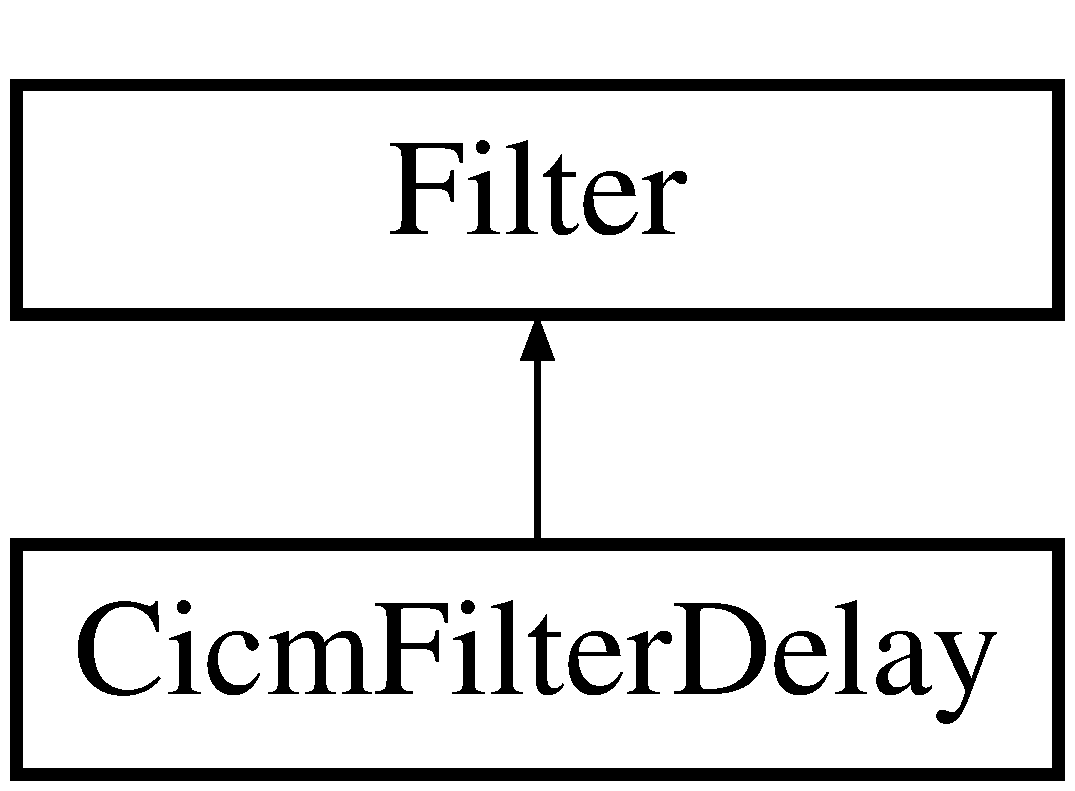
\includegraphics[height=2.000000cm]{class_cicm_filter_delay}
\end{center}
\end{figure}


The documentation for this class was generated from the following files\-:\begin{DoxyCompactItemize}
\item 
/\-Users/\-Pierre/\-Source\-Tree/\-Hoa\-Library/\-Sources/\-Cicm\-Library/\-Cicm\-Filters/Cicm\-Filter\-Delay.\-h\item 
/\-Users/\-Pierre/\-Source\-Tree/\-Hoa\-Library/\-Sources/\-Cicm\-Library/\-Cicm\-Filters/Cicm\-Filter\-Delay.\-cpp\end{DoxyCompactItemize}

\hypertarget{class_cicm_line}{\section{Cicm\-Line Class Reference}
\label{class_cicm_line}\index{Cicm\-Line@{Cicm\-Line}}
}


The documentation for this class was generated from the following files\-:\begin{DoxyCompactItemize}
\item 
/\-Users/\-Pierre/\-Source\-Tree/\-Hoa\-Library/\-Sources/\-Cicm\-Library/\-Cicm\-Lines/Cicm\-Line.\-h\item 
/\-Users/\-Pierre/\-Source\-Tree/\-Hoa\-Library/\-Sources/\-Cicm\-Library/\-Cicm\-Lines/Cicm\-Line.\-cpp\end{DoxyCompactItemize}

\hypertarget{class_cicm_qsgs}{\section{Cicm\-Qsgs Class Reference}
\label{class_cicm_qsgs}\index{Cicm\-Qsgs@{Cicm\-Qsgs}}
}


\subsection{Detailed Description}


Definition at line 37 of file Cicm\-Q\-S\-G\-S.\-h.



The documentation for this class was generated from the following files\-:\begin{DoxyCompactItemize}
\item 
/\-Users/\-Pierre/\-Source\-Tree/\-Hoa\-Library/\-Sources/\-Cicm\-Library/\-Cicm\-Granular/Cicm\-Q\-S\-G\-S.\-h\item 
/\-Users/\-Pierre/\-Source\-Tree/\-Hoa\-Library/\-Sources/\-Cicm\-Library/\-Cicm\-Granular/Cicm\-Q\-S\-G\-S.\-cpp\end{DoxyCompactItemize}

\hypertarget{class_cicm_ring_modulation}{\section{Cicm\-Ring\-Modulation Class Reference}
\label{class_cicm_ring_modulation}\index{Cicm\-Ring\-Modulation@{Cicm\-Ring\-Modulation}}
}
\subsection*{Public Member Functions}
\begin{DoxyCompactItemize}
\item 
\hypertarget{class_cicm_ring_modulation_a421451721b34a88a1df6e2e072556527}{{\bfseries Cicm\-Ring\-Modulation} (long a\-Vector\-Size=1, double a\-Sampling\-Rate=44100.)}\label{class_cicm_ring_modulation_a421451721b34a88a1df6e2e072556527}

\item 
\hypertarget{class_cicm_ring_modulation_a15390c47bc280fd0283e77d1cfc1b8cc}{void {\bfseries set\-Vector\-Size} (long a\-Vector\-Size)}\label{class_cicm_ring_modulation_a15390c47bc280fd0283e77d1cfc1b8cc}

\item 
\hypertarget{class_cicm_ring_modulation_ad4a4f349aebabf28e7b34679252c4dac}{void {\bfseries set\-Sampling\-Rate} (long a\-Sampling\-Rate)}\label{class_cicm_ring_modulation_ad4a4f349aebabf28e7b34679252c4dac}

\item 
\hypertarget{class_cicm_ring_modulation_ad90a8da25392efc63d7afd338acf41c9}{void {\bfseries set\-Frequency} (double a\-Frequency)}\label{class_cicm_ring_modulation_ad90a8da25392efc63d7afd338acf41c9}

\item 
\hypertarget{class_cicm_ring_modulation_a44bbcbf21be8c1988f1d75613f8a0467}{long {\bfseries get\-Vector\-Size} ()}\label{class_cicm_ring_modulation_a44bbcbf21be8c1988f1d75613f8a0467}

\item 
\hypertarget{class_cicm_ring_modulation_a2087da92c5111c19dd3f0959582e4b26}{long {\bfseries get\-Sampling\-Rate} ()}\label{class_cicm_ring_modulation_a2087da92c5111c19dd3f0959582e4b26}

\item 
\hypertarget{class_cicm_ring_modulation_a38eea5039c3402b3f140b71544cbdf60}{double {\bfseries get\-Frequency} ()}\label{class_cicm_ring_modulation_a38eea5039c3402b3f140b71544cbdf60}

\item 
\hypertarget{class_cicm_ring_modulation_aad65214bebc99186a72555eca8875a23}{float {\bfseries process} (float input)}\label{class_cicm_ring_modulation_aad65214bebc99186a72555eca8875a23}

\item 
\hypertarget{class_cicm_ring_modulation_af46c753c9e55989a42099f737d810340}{double {\bfseries process} (double input)}\label{class_cicm_ring_modulation_af46c753c9e55989a42099f737d810340}

\item 
\hypertarget{class_cicm_ring_modulation_aa7c8cbc4e28c9158689ef5c84846dcbb}{void {\bfseries process} (float $\ast$inputs, float $\ast$outputs)}\label{class_cicm_ring_modulation_aa7c8cbc4e28c9158689ef5c84846dcbb}

\item 
\hypertarget{class_cicm_ring_modulation_a7fe5d1310b4959648c788427c57e9d9a}{void {\bfseries process} (double $\ast$inputs, double $\ast$outputs)}\label{class_cicm_ring_modulation_a7fe5d1310b4959648c788427c57e9d9a}

\end{DoxyCompactItemize}
\subsection*{Protected Attributes}
\begin{DoxyCompactItemize}
\item 
\hypertarget{class_cicm_ring_modulation_a595019f0de136109a20b2f20b5995eff}{\hyperlink{class_cicm_line}{Cicm\-Line} $\ast$ {\bfseries m\-\_\-line}}\label{class_cicm_ring_modulation_a595019f0de136109a20b2f20b5995eff}

\item 
\hypertarget{class_cicm_ring_modulation_afb39ee82ab804e7f2b03aa3e796910a5}{\hyperlink{class_cicm_envelope}{Cicm\-Envelope} $\ast$ {\bfseries m\-\_\-envelope}}\label{class_cicm_ring_modulation_afb39ee82ab804e7f2b03aa3e796910a5}

\item 
\hypertarget{class_cicm_ring_modulation_a6434dc1562bd2f4bdcb76c946cca53a2}{long {\bfseries m\-\_\-vector\-\_\-size}}\label{class_cicm_ring_modulation_a6434dc1562bd2f4bdcb76c946cca53a2}

\item 
\hypertarget{class_cicm_ring_modulation_ac531f1e2606e838578610000834ecbab}{long {\bfseries m\-\_\-sampling\-\_\-rate}}\label{class_cicm_ring_modulation_ac531f1e2606e838578610000834ecbab}

\item 
\hypertarget{class_cicm_ring_modulation_ac430d37962411e406695f772f11985b8}{double {\bfseries m\-\_\-frequency}}\label{class_cicm_ring_modulation_ac430d37962411e406695f772f11985b8}

\end{DoxyCompactItemize}


The documentation for this class was generated from the following files\-:\begin{DoxyCompactItemize}
\item 
/\-Users/\-Pierre/\-Source\-Tree/\-Hoa\-Library/\-Sources/\-Cicm\-Library/\-Cicm\-Amplitude/Cicm\-Ring\-Modulation.\-h\item 
/\-Users/\-Pierre/\-Source\-Tree/\-Hoa\-Library/\-Sources/\-Cicm\-Library/\-Cicm\-Amplitude/Cicm\-Ring\-Modulation.\-cpp\end{DoxyCompactItemize}

\hypertarget{structcolor}{\section{color Struct Reference}
\label{structcolor}\index{color@{color}}
}


\subsection{Detailed Description}


Definition at line 86 of file Cicm\-Tools.\-h.



The documentation for this struct was generated from the following file\-:\begin{DoxyCompactItemize}
\item 
/\-Users/\-Pierre/\-Source\-Tree/\-Hoa\-Library/\-Sources/\-Cicm\-Library/Cicm\-Tools.\-h\end{DoxyCompactItemize}

\hypertarget{structcoordinates_cartesian}{\section{coordinates\-Cartesian Struct Reference}
\label{structcoordinates_cartesian}\index{coordinates\-Cartesian@{coordinates\-Cartesian}}
}


\subsection{Detailed Description}


Definition at line 80 of file Cicm\-Tools.\-h.



The documentation for this struct was generated from the following file\-:\begin{DoxyCompactItemize}
\item 
/\-Users/\-Pierre/\-Source\-Tree/\-Hoa\-Library/\-Sources/\-Cicm\-Library/Cicm\-Tools.\-h\end{DoxyCompactItemize}

\hypertarget{structcoordinates_polar}{\section{coordinates\-Polar Struct Reference}
\label{structcoordinates_polar}\index{coordinates\-Polar@{coordinates\-Polar}}
}


\subsection{Detailed Description}


Definition at line 74 of file Cicm\-Tools.\-h.



The documentation for this struct was generated from the following file\-:\begin{DoxyCompactItemize}
\item 
/\-Users/\-Pierre/\-Source\-Tree/\-Hoa\-Library/\-Sources/\-Cicm\-Library/Cicm\-Tools.\-h\end{DoxyCompactItemize}

\hypertarget{class_filter}{\section{Filter Class Reference}
\label{class_filter}\index{Filter@{Filter}}
}
Inheritance diagram for Filter\-:\begin{figure}[H]
\begin{center}
\leavevmode
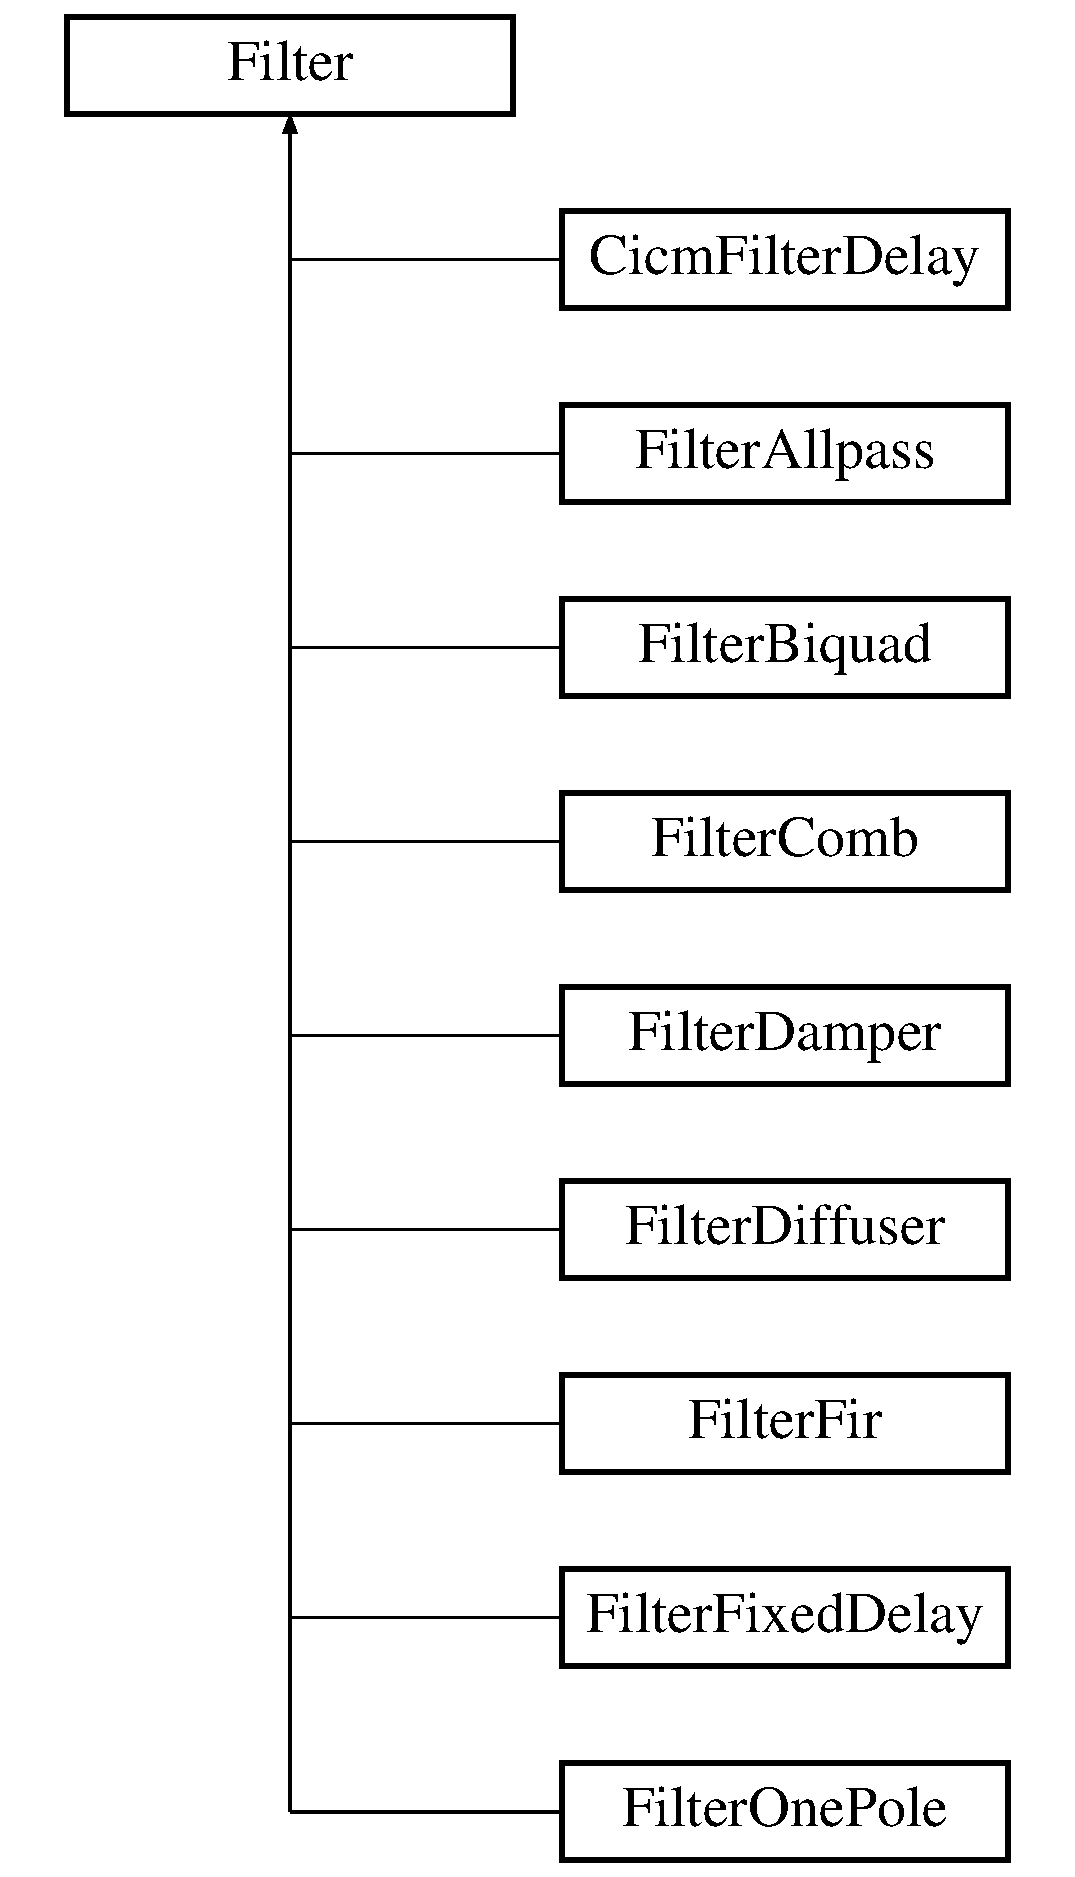
\includegraphics[height=10.000000cm]{class_filter}
\end{center}
\end{figure}
\subsection*{Public Member Functions}
\begin{DoxyCompactItemize}
\item 
\hypertarget{class_filter_a5c6deec2210aaa2664d512ec35a5dfc0}{{\bfseries Filter} (long a\-Vector\-Size=0, long a\-Sampling\-Rate=44100)}\label{class_filter_a5c6deec2210aaa2664d512ec35a5dfc0}

\item 
\hypertarget{class_filter_aa8f928748937e51095a22ce29c9c08c4}{long {\bfseries get\-Vector\-Size} ()}\label{class_filter_aa8f928748937e51095a22ce29c9c08c4}

\item 
\hypertarget{class_filter_aceb44fa5badb70e5f35fd7388288650b}{long {\bfseries get\-Sampling\-Rate} ()}\label{class_filter_aceb44fa5badb70e5f35fd7388288650b}

\item 
\hypertarget{class_filter_a8ee16a822086b1a96ac6b625c77d923d}{void {\bfseries set\-Vector\-Size} (long a\-Vector\-Size)}\label{class_filter_a8ee16a822086b1a96ac6b625c77d923d}

\item 
\hypertarget{class_filter_a02c21fa49f5a8837a1ece9db10722493}{void {\bfseries set\-Sampling\-Rate} (long a\-Sampling\-Rate)}\label{class_filter_a02c21fa49f5a8837a1ece9db10722493}

\item 
\hypertarget{class_filter_ac7f8d9d379dcc40e98d4204eac023f22}{float {\bfseries process} (float input)}\label{class_filter_ac7f8d9d379dcc40e98d4204eac023f22}

\item 
\hypertarget{class_filter_a2379f87a7f71d76069abfcc090aaa24c}{double {\bfseries process} (double input)}\label{class_filter_a2379f87a7f71d76069abfcc090aaa24c}

\item 
\hypertarget{class_filter_a250100634bd88b32db92b248cc49d2d7}{void {\bfseries process} (float $\ast$inputs, float $\ast$outputs)}\label{class_filter_a250100634bd88b32db92b248cc49d2d7}

\item 
\hypertarget{class_filter_ab5c77fb6f129588d6b1fedb51de1b12e}{void {\bfseries process} (double $\ast$inputs, double $\ast$outputs)}\label{class_filter_ab5c77fb6f129588d6b1fedb51de1b12e}

\end{DoxyCompactItemize}
\subsection*{Protected Attributes}
\begin{DoxyCompactItemize}
\item 
\hypertarget{class_filter_af9ca666c9fe182e676238dac04429954}{long {\bfseries m\-\_\-vector\-\_\-size}}\label{class_filter_af9ca666c9fe182e676238dac04429954}

\item 
\hypertarget{class_filter_a320edddf1bc2586ac19c9f5cd833bd82}{long {\bfseries m\-\_\-sampling\-\_\-rate}}\label{class_filter_a320edddf1bc2586ac19c9f5cd833bd82}

\end{DoxyCompactItemize}


The documentation for this class was generated from the following files\-:\begin{DoxyCompactItemize}
\item 
/\-Users/\-Pierre/\-Source\-Tree/\-Hoa\-Library/\-Sources/\-Cicm\-Library/\-Cicm\-Filters/Cicm\-Filter.\-h\item 
/\-Users/\-Pierre/\-Source\-Tree/\-Hoa\-Library/\-Sources/\-Cicm\-Library/\-Cicm\-Filters/Cicm\-Filter.\-cpp\end{DoxyCompactItemize}

\hypertarget{class_filter_allpass}{\section{Filter\-Allpass Class Reference}
\label{class_filter_allpass}\index{Filter\-Allpass@{Filter\-Allpass}}
}
Inheritance diagram for Filter\-Allpass\-:\begin{figure}[H]
\begin{center}
\leavevmode
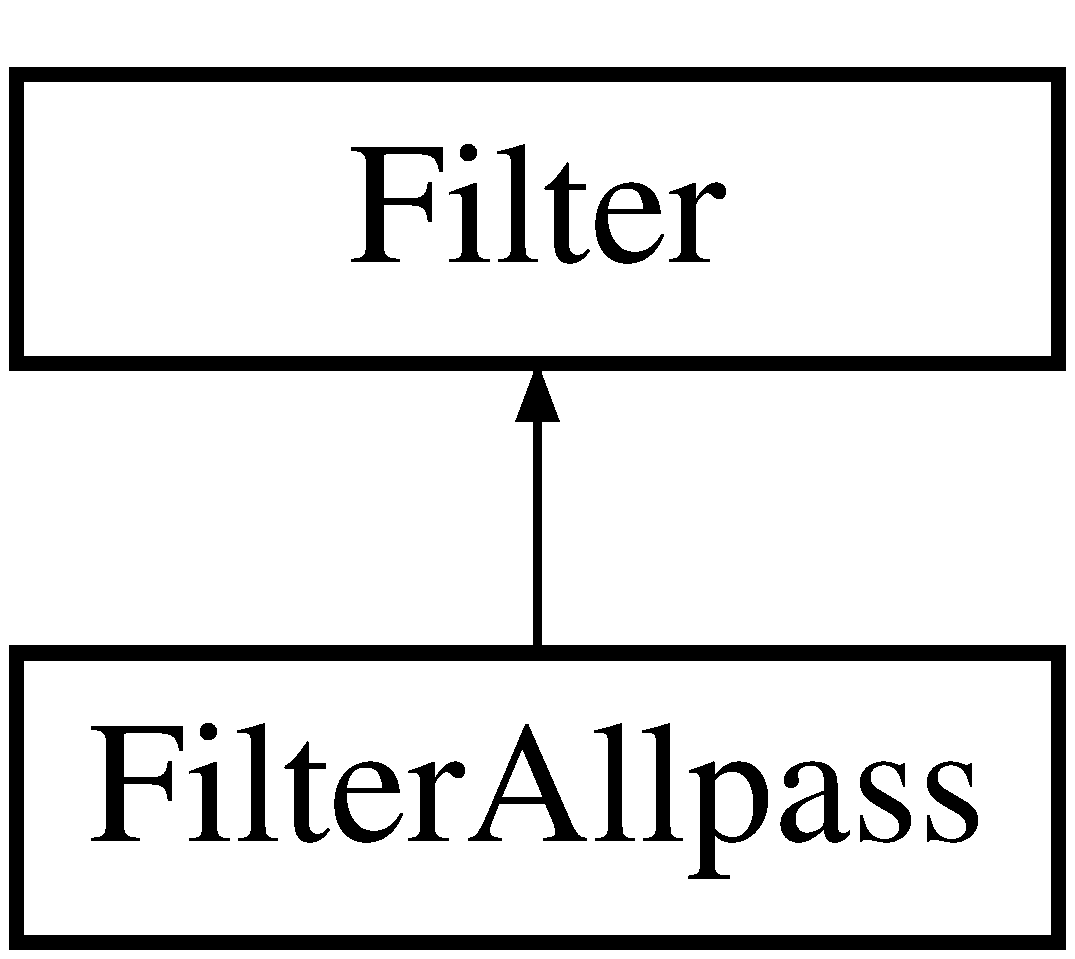
\includegraphics[height=2.000000cm]{class_filter_allpass}
\end{center}
\end{figure}
\subsection*{Public Member Functions}
\begin{DoxyCompactItemize}
\item 
\hypertarget{class_filter_allpass_a7bad6e9dd0bc3e2a8e67a6ba287243e9}{{\bfseries Filter\-Allpass} (long a\-Buffer\-Size)}\label{class_filter_allpass_a7bad6e9dd0bc3e2a8e67a6ba287243e9}

\item 
\hypertarget{class_filter_allpass_a8dff846eca0d606c07a91b348b265372}{void {\bfseries set\-Buffer\-Size\-Max} (long a\-Buffer\-Size)}\label{class_filter_allpass_a8dff846eca0d606c07a91b348b265372}

\item 
\hypertarget{class_filter_allpass_accafa192c6264a5e080b68835feabab9}{long {\bfseries get\-Buffer\-Size\-Max} ()}\label{class_filter_allpass_accafa192c6264a5e080b68835feabab9}

\item 
\hypertarget{class_filter_allpass_a8f5ad43d883643d482c65541e65548ba}{void {\bfseries set\-Buffer\-Size} (long a\-Buffer\-Size)}\label{class_filter_allpass_a8f5ad43d883643d482c65541e65548ba}

\item 
\hypertarget{class_filter_allpass_aff058f1fe7aea8c09ef31ca2f61915ce}{long {\bfseries get\-Buffer\-Size} ()}\label{class_filter_allpass_aff058f1fe7aea8c09ef31ca2f61915ce}

\item 
\hypertarget{class_filter_allpass_a4449cf1c74613e5dfddceb6f611b2793}{void {\bfseries set\-Feedback} (double val)}\label{class_filter_allpass_a4449cf1c74613e5dfddceb6f611b2793}

\item 
\hypertarget{class_filter_allpass_a8d25f65d21b66d617fe5239479311d17}{double {\bfseries get\-Feedback} ()}\label{class_filter_allpass_a8d25f65d21b66d617fe5239479311d17}

\item 
\hypertarget{class_filter_allpass_a205d78909b64f59f68246e1c1841ee21}{double {\bfseries process} (const double an\-Input)}\label{class_filter_allpass_a205d78909b64f59f68246e1c1841ee21}

\item 
\hypertarget{class_filter_allpass_aac8495bc5fc5c01ec3c5767447e281cf}{float {\bfseries process} (const float an\-Input)}\label{class_filter_allpass_aac8495bc5fc5c01ec3c5767447e281cf}

\end{DoxyCompactItemize}
\subsection*{Additional Inherited Members}


The documentation for this class was generated from the following files\-:\begin{DoxyCompactItemize}
\item 
/\-Users/\-Pierre/\-Source\-Tree/\-Hoa\-Library/\-Sources/\-Cicm\-Library/\-Cicm\-Filters/Cicm\-Filter\-Allpass.\-h\item 
/\-Users/\-Pierre/\-Source\-Tree/\-Hoa\-Library/\-Sources/\-Cicm\-Library/\-Cicm\-Filters/Cicm\-Filter\-Allpass.\-cpp\end{DoxyCompactItemize}

\hypertarget{class_filter_biquad}{\section{Filter\-Biquad Class Reference}
\label{class_filter_biquad}\index{Filter\-Biquad@{Filter\-Biquad}}
}
Inheritance diagram for Filter\-Biquad\-:\begin{figure}[H]
\begin{center}
\leavevmode
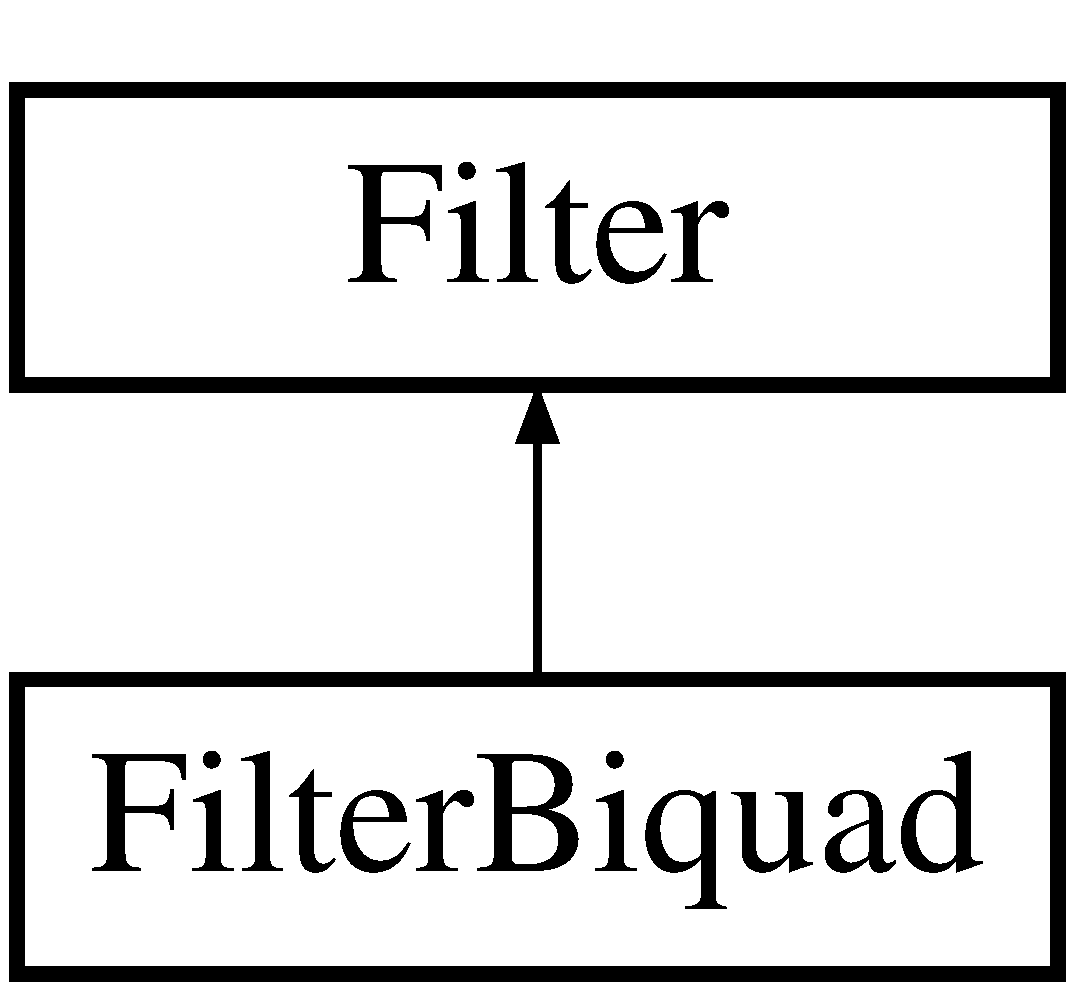
\includegraphics[height=2.000000cm]{class_filter_biquad}
\end{center}
\end{figure}


\subsection{Detailed Description}


Definition at line 42 of file Cicm\-Filter\-Biquad.\-h.



The documentation for this class was generated from the following files\-:\begin{DoxyCompactItemize}
\item 
/\-Users/\-Pierre/\-Source\-Tree/\-Hoa\-Library/\-Sources/\-Cicm\-Library/\-Cicm\-Filters/Cicm\-Filter\-Biquad.\-h\item 
/\-Users/\-Pierre/\-Source\-Tree/\-Hoa\-Library/\-Sources/\-Cicm\-Library/\-Cicm\-Filters/Cicm\-Filter\-Biquad.\-cpp\end{DoxyCompactItemize}

\hypertarget{class_filter_comb}{\section{Filter\-Comb Class Reference}
\label{class_filter_comb}\index{Filter\-Comb@{Filter\-Comb}}
}


{\ttfamily \#include $<$Cicm\-Filter\-Comb.\-h$>$}

Inheritance diagram for Filter\-Comb\-:\begin{figure}[H]
\begin{center}
\leavevmode
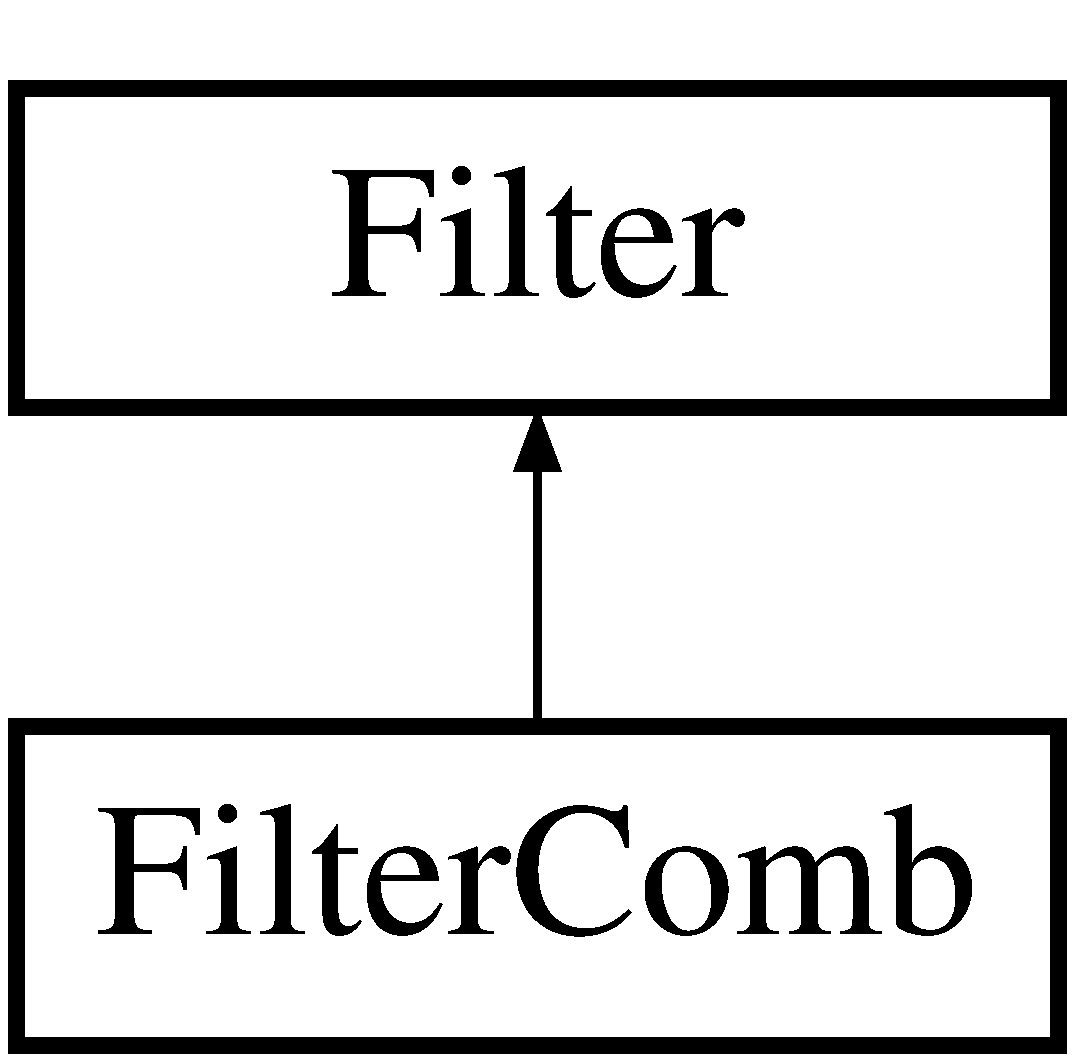
\includegraphics[height=2.000000cm]{class_filter_comb}
\end{center}
\end{figure}


\subsection{Detailed Description}
y(n) = a $\ast$ x(n) + b $\ast$ x(n-\/delay) + c $\ast$ y(n-\/delay) 

Definition at line 35 of file Cicm\-Filter\-Comb.\-h.



The documentation for this class was generated from the following files\-:\begin{DoxyCompactItemize}
\item 
/\-Users/\-Pierre/\-Source\-Tree/\-Hoa\-Library/\-Sources/\-Cicm\-Library/\-Cicm\-Filters/Cicm\-Filter\-Comb.\-h\item 
/\-Users/\-Pierre/\-Source\-Tree/\-Hoa\-Library/\-Sources/\-Cicm\-Library/\-Cicm\-Filters/Cicm\-Filter\-Comb.\-cpp\end{DoxyCompactItemize}

\hypertarget{class_filter_convolution}{\section{Filter\-Convolution Class Reference}
\label{class_filter_convolution}\index{Filter\-Convolution@{Filter\-Convolution}}
}


\subsection{Detailed Description}


Definition at line 33 of file Cicm\-Filter\-Convolution.\-h.



The documentation for this class was generated from the following files\-:\begin{DoxyCompactItemize}
\item 
/\-Users/elioton/\-Documents/programmation/\-C\-I\-C\-M/source\-Tree/\-Hoa\-Library/\-Sources/\-Cicm\-Library/\-Cicm\-Filters/Cicm\-Filter\-Convolution.\-h\item 
/\-Users/elioton/\-Documents/programmation/\-C\-I\-C\-M/source\-Tree/\-Hoa\-Library/\-Sources/\-Cicm\-Library/\-Cicm\-Filters/Cicm\-Filter\-Convolution.\-cpp\end{DoxyCompactItemize}

\hypertarget{class_filter_convolution_zero}{\section{Filter\-Convolution\-Zero Class Reference}
\label{class_filter_convolution_zero}\index{Filter\-Convolution\-Zero@{Filter\-Convolution\-Zero}}
}
\subsection*{Public Member Functions}
\begin{DoxyCompactItemize}
\item 
\hypertarget{class_filter_convolution_zero_ad8b99b17449c1f06f63679ff0f0f9daf}{{\bfseries Filter\-Convolution\-Zero} (long a\-Minimum\-Size=128, long a\-Maximum\-Size=32768)}\label{class_filter_convolution_zero_ad8b99b17449c1f06f63679ff0f0f9daf}

\item 
\hypertarget{class_filter_convolution_zero_a8beb3fe66957237230d49bf0c29c7a6a}{void {\bfseries set\-Impulse\-Response} (float $\ast$an\-Impul\-Response, long a\-Size)}\label{class_filter_convolution_zero_a8beb3fe66957237230d49bf0c29c7a6a}

\item 
\hypertarget{class_filter_convolution_zero_a99587aba1900a8321fc8dce7bc9f1c61}{void {\bfseries clear} ()}\label{class_filter_convolution_zero_a99587aba1900a8321fc8dce7bc9f1c61}

\item 
\hypertarget{class_filter_convolution_zero_a5ac3b6f34c2abf7d74547f5a49b349d8}{long {\bfseries get\-Number\-Of\-F\-F\-Ts} ()}\label{class_filter_convolution_zero_a5ac3b6f34c2abf7d74547f5a49b349d8}

\item 
\hypertarget{class_filter_convolution_zero_a17f92e18bd1f8bd10a5efc7bc6c1510c}{long {\bfseries get\-Number\-Of\-Instance} ()}\label{class_filter_convolution_zero_a17f92e18bd1f8bd10a5efc7bc6c1510c}

\item 
\hypertarget{class_filter_convolution_zero_a96938a69a33f3a9c85f3c2ce21e7e40f}{double {\bfseries process} (const double input)}\label{class_filter_convolution_zero_a96938a69a33f3a9c85f3c2ce21e7e40f}

\item 
\hypertarget{class_filter_convolution_zero_a8a6f23806e836d06ef8aaa4aebaded38}{float {\bfseries process} (const float input)}\label{class_filter_convolution_zero_a8a6f23806e836d06ef8aaa4aebaded38}

\end{DoxyCompactItemize}
\subsection*{Protected Attributes}
\begin{DoxyCompactItemize}
\item 
\hypertarget{class_filter_convolution_zero_a8db018405cb92c917d02f20d45b2dd65}{int {\bfseries m\-\_\-minimum\-\_\-size}}\label{class_filter_convolution_zero_a8db018405cb92c917d02f20d45b2dd65}

\item 
\hypertarget{class_filter_convolution_zero_add9e349da32a20fd6186edb0e28b92fc}{int {\bfseries m\-\_\-maximum\-\_\-size}}\label{class_filter_convolution_zero_add9e349da32a20fd6186edb0e28b92fc}

\item 
\hypertarget{class_filter_convolution_zero_a9069f23a84d1c2f46f2c640e5be61897}{int {\bfseries m\-\_\-number\-\_\-of\-\_\-ffts}}\label{class_filter_convolution_zero_a9069f23a84d1c2f46f2c640e5be61897}

\item 
\hypertarget{class_filter_convolution_zero_a4e6d5c985380124f57b86ab70bbe509c}{int {\bfseries m\-\_\-ffts\-\_\-useds}}\label{class_filter_convolution_zero_a4e6d5c985380124f57b86ab70bbe509c}

\item 
\hypertarget{class_filter_convolution_zero_a201baa7ff84ae7b09df236627de03448}{\hyperlink{class_filter_fir}{Filter\-Fir} $\ast$ {\bfseries m\-\_\-fir}}\label{class_filter_convolution_zero_a201baa7ff84ae7b09df236627de03448}

\item 
\hypertarget{class_filter_convolution_zero_a03a3c81b87a781da55a97dd40aacdd68}{vector$<$ \hyperlink{class_filter_convolution}{Filter\-Convolution} $\ast$ $>$ {\bfseries m\-\_\-fft}}\label{class_filter_convolution_zero_a03a3c81b87a781da55a97dd40aacdd68}

\end{DoxyCompactItemize}


The documentation for this class was generated from the following files\-:\begin{DoxyCompactItemize}
\item 
/\-Users/\-Pierre/\-Source\-Tree/\-Hoa\-Library/\-Sources/\-Cicm\-Library/\-Cicm\-Filters/Cicm\-Filter\-Convolution\-Zero.\-h\item 
/\-Users/\-Pierre/\-Source\-Tree/\-Hoa\-Library/\-Sources/\-Cicm\-Library/\-Cicm\-Filters/Cicm\-Filter\-Convolution\-Zero.\-cpp\end{DoxyCompactItemize}

\hypertarget{class_filter_damper}{\section{Filter\-Damper Class Reference}
\label{class_filter_damper}\index{Filter\-Damper@{Filter\-Damper}}
}
Inheritance diagram for Filter\-Damper\-:\begin{figure}[H]
\begin{center}
\leavevmode
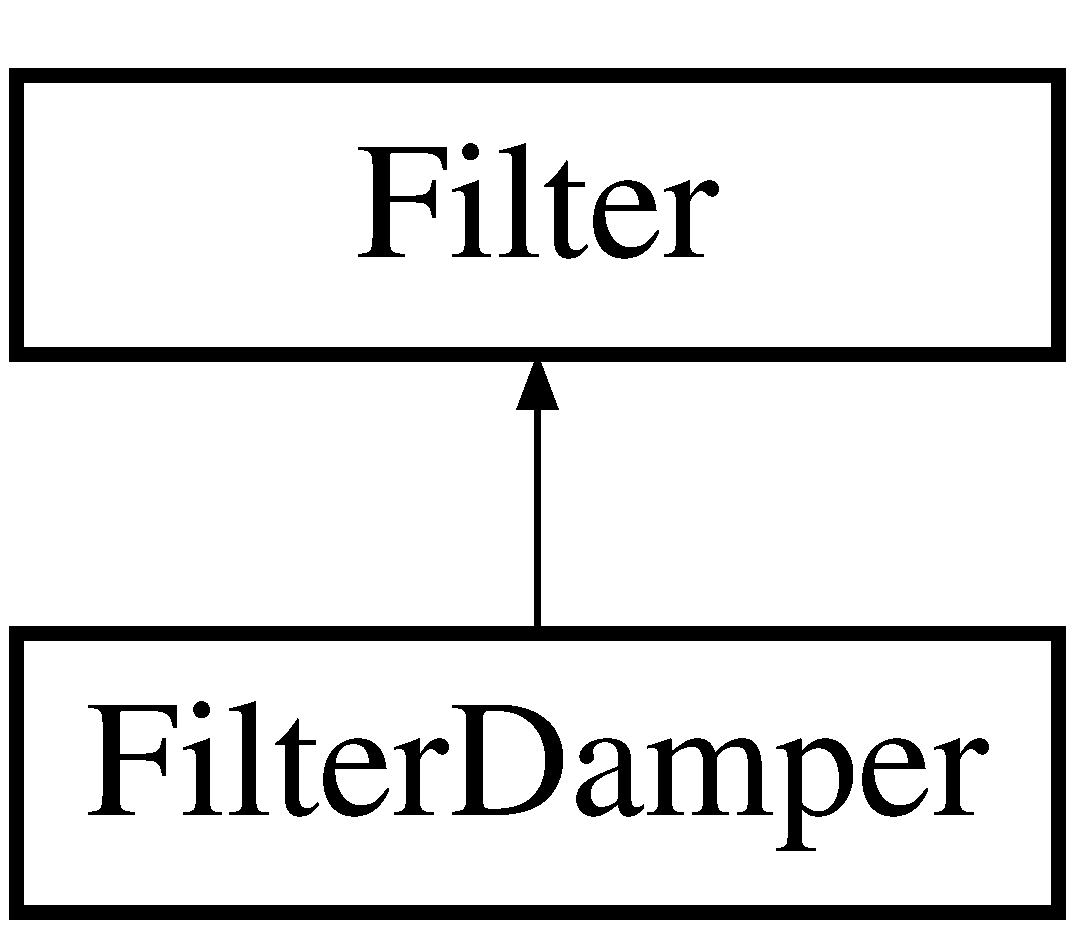
\includegraphics[height=2.000000cm]{class_filter_damper}
\end{center}
\end{figure}


The documentation for this class was generated from the following file\-:\begin{DoxyCompactItemize}
\item 
/\-Users/\-Pierre/\-Source\-Tree/\-Hoa\-Library/\-Sources/\-Cicm\-Library/\-Cicm\-Filters/Cicm\-Filter\-Damper.\-h\end{DoxyCompactItemize}

\hypertarget{class_filter_diffuser}{\section{Filter\-Diffuser Class Reference}
\label{class_filter_diffuser}\index{Filter\-Diffuser@{Filter\-Diffuser}}
}
Inheritance diagram for Filter\-Diffuser\-:\begin{figure}[H]
\begin{center}
\leavevmode
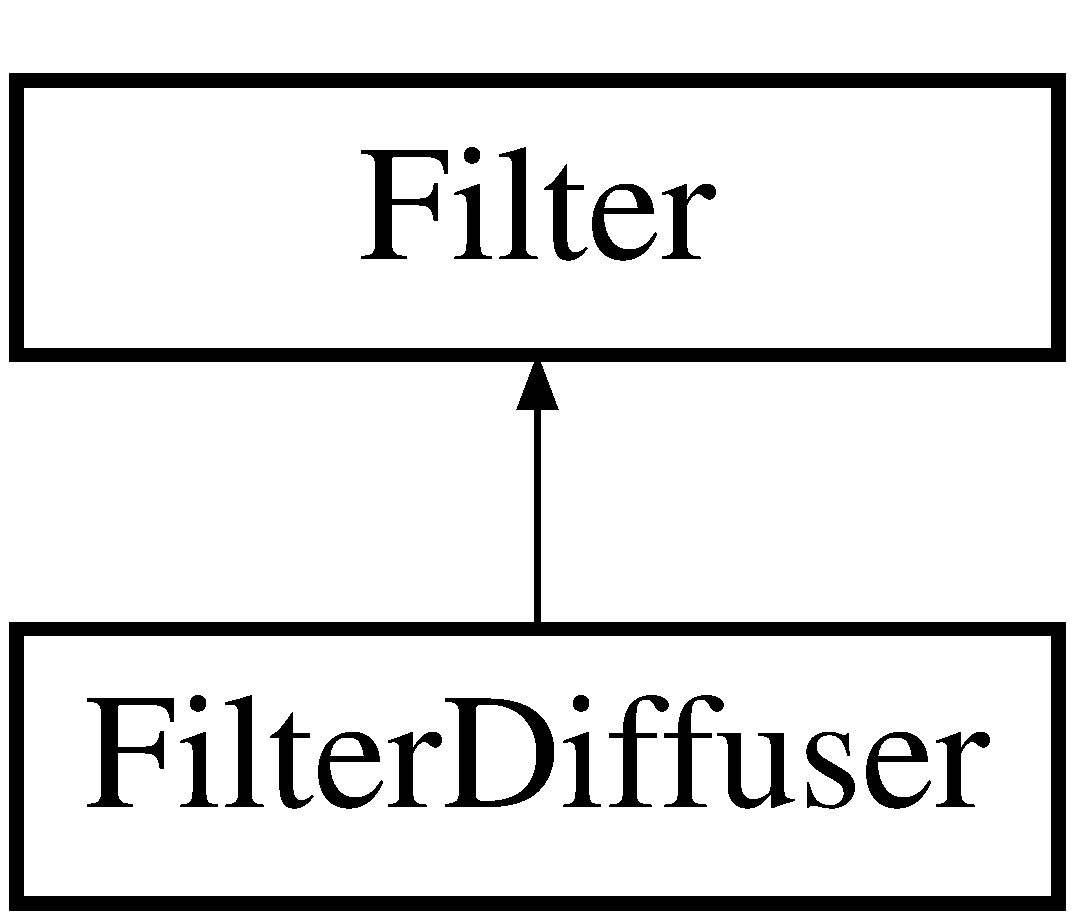
\includegraphics[height=2.000000cm]{class_filter_diffuser}
\end{center}
\end{figure}


\subsection{Detailed Description}


Definition at line 31 of file Cicm\-Filter\-Diffuser.\-h.



The documentation for this class was generated from the following files\-:\begin{DoxyCompactItemize}
\item 
/\-Users/elioton/\-Documents/programmation/\-C\-I\-C\-M/source\-Tree/\-Hoa\-Library/\-Sources/\-Cicm\-Library/\-Cicm\-Filters/Cicm\-Filter\-Diffuser.\-h\item 
/\-Users/elioton/\-Documents/programmation/\-C\-I\-C\-M/source\-Tree/\-Hoa\-Library/\-Sources/\-Cicm\-Library/\-Cicm\-Filters/Cicm\-Filter\-Diffuser.\-cpp\end{DoxyCompactItemize}

\hypertarget{class_filter_fir}{\section{Filter\-Fir Class Reference}
\label{class_filter_fir}\index{Filter\-Fir@{Filter\-Fir}}
}
Inheritance diagram for Filter\-Fir\-:\begin{figure}[H]
\begin{center}
\leavevmode
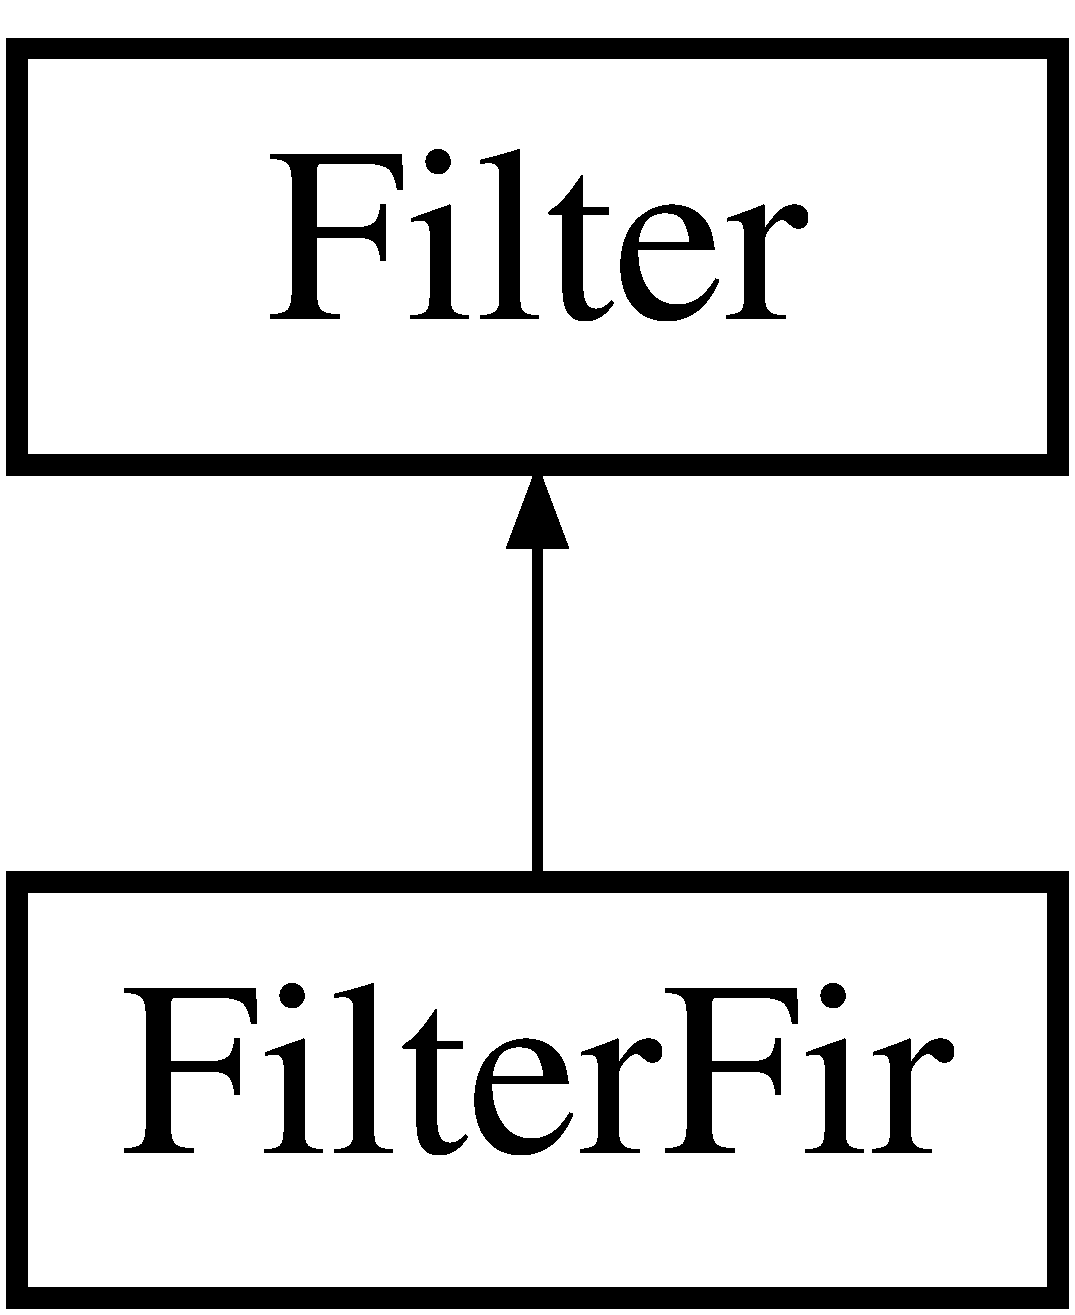
\includegraphics[height=2.000000cm]{class_filter_fir}
\end{center}
\end{figure}


The documentation for this class was generated from the following files\-:\begin{DoxyCompactItemize}
\item 
/\-Users/\-Pierre/\-Source\-Tree/\-Hoa\-Library/\-Sources/\-Cicm\-Library/\-Cicm\-Filters/Cicm\-Filter\-Fir.\-h\item 
/\-Users/\-Pierre/\-Source\-Tree/\-Hoa\-Library/\-Sources/\-Cicm\-Library/\-Cicm\-Filters/Cicm\-Filter\-Fir.\-cpp\end{DoxyCompactItemize}

\hypertarget{class_filter_fixed_delay}{\section{Filter\-Fixed\-Delay Class Reference}
\label{class_filter_fixed_delay}\index{Filter\-Fixed\-Delay@{Filter\-Fixed\-Delay}}
}
Inheritance diagram for Filter\-Fixed\-Delay\-:\begin{figure}[H]
\begin{center}
\leavevmode
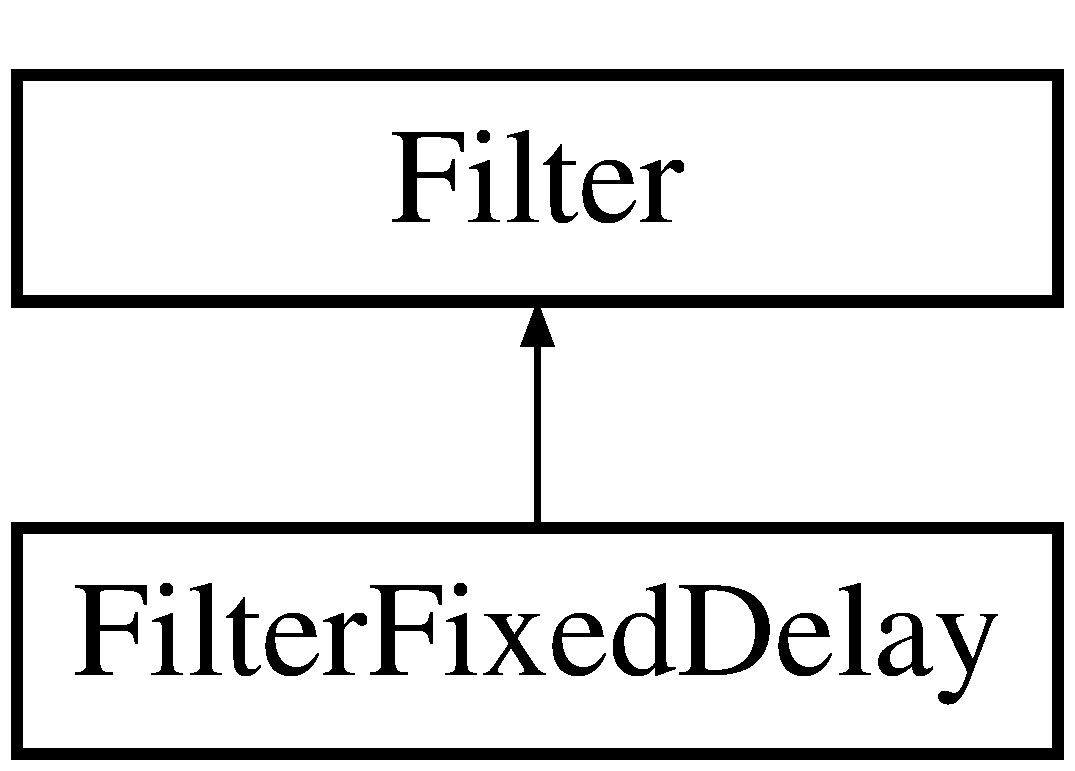
\includegraphics[height=2.000000cm]{class_filter_fixed_delay}
\end{center}
\end{figure}


The documentation for this class was generated from the following files\-:\begin{DoxyCompactItemize}
\item 
/\-Users/\-Pierre/\-Source\-Tree/\-Hoa\-Library/\-Sources/\-Cicm\-Library/\-Cicm\-Filters/Cicm\-Filter\-Fixed\-Delay.\-h\item 
/\-Users/\-Pierre/\-Source\-Tree/\-Hoa\-Library/\-Sources/\-Cicm\-Library/\-Cicm\-Filters/Cicm\-Filter\-Fixed\-Delay.\-cpp\end{DoxyCompactItemize}

\hypertarget{class_filter_one_pole}{\section{Filter\-One\-Pole Class Reference}
\label{class_filter_one_pole}\index{Filter\-One\-Pole@{Filter\-One\-Pole}}
}


{\ttfamily \#include $<$Cicm\-Filter\-One\-Pole.\-h$>$}

Inheritance diagram for Filter\-One\-Pole\-:\begin{figure}[H]
\begin{center}
\leavevmode
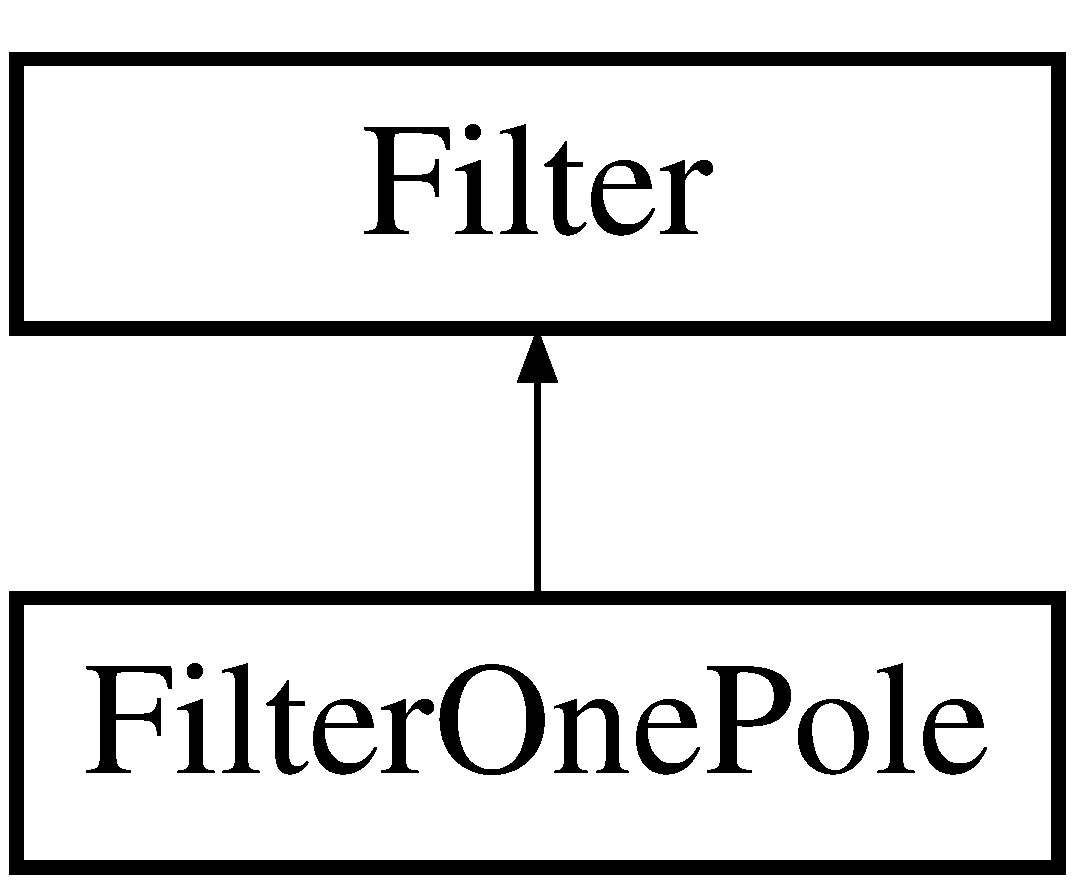
\includegraphics[height=2.000000cm]{class_filter_one_pole}
\end{center}
\end{figure}
\subsection*{Public Member Functions}
\begin{DoxyCompactItemize}
\item 
\hyperlink{class_filter_one_pole_aa420e43a875791fa5332aaa3d5654f5a}{Filter\-One\-Pole} (double a\-Sampling\-Rate=44100, long a\-Vector\-Size=0)
\item 
\hypertarget{class_filter_one_pole_a118ec1e24997eb8603f34f30f8fd06a5}{void {\bfseries set\-Sampling\-Rate} (double a\-Sampling\-Rate)}\label{class_filter_one_pole_a118ec1e24997eb8603f34f30f8fd06a5}

\item 
\hypertarget{class_filter_one_pole_ab44016c3073687e627d9196c07ddb494}{void {\bfseries set\-Coeff\-A} (double a\-Coefficient)}\label{class_filter_one_pole_ab44016c3073687e627d9196c07ddb494}

\item 
\hypertarget{class_filter_one_pole_a0ae3f86d4d9d2ce37fa020e6f15942f6}{void {\bfseries set\-Coeff\-B} (double a\-Coefficient)}\label{class_filter_one_pole_a0ae3f86d4d9d2ce37fa020e6f15942f6}

\item 
\hypertarget{class_filter_one_pole_a322259144e6df23695578991234a4561}{void {\bfseries set\-Cut\-Off\-Frequency} (double a\-Frequency)}\label{class_filter_one_pole_a322259144e6df23695578991234a4561}

\item 
\hypertarget{class_filter_one_pole_a5edb88ff5424eb6cadf16be1316770b1}{double {\bfseries get\-Coeff\-A} ()}\label{class_filter_one_pole_a5edb88ff5424eb6cadf16be1316770b1}

\item 
\hypertarget{class_filter_one_pole_ab746acf7c5a865d3145856aa0edb8ff1}{double {\bfseries get\-Coeff\-B} ()}\label{class_filter_one_pole_ab746acf7c5a865d3145856aa0edb8ff1}

\item 
\hypertarget{class_filter_one_pole_a8e3e803096cb900f7f822f9b8359b447}{double {\bfseries get\-Cut\-Off\-Frequency} ()}\label{class_filter_one_pole_a8e3e803096cb900f7f822f9b8359b447}

\item 
\hypertarget{class_filter_one_pole_a1f137013e13ccb09916c1a300af8c043}{double {\bfseries process} (double a\-Sample)}\label{class_filter_one_pole_a1f137013e13ccb09916c1a300af8c043}

\item 
\hypertarget{class_filter_one_pole_ad558f13f57747ecddcf0d652f25549f6}{float {\bfseries process} (float a\-Sample)}\label{class_filter_one_pole_ad558f13f57747ecddcf0d652f25549f6}

\item 
\hypertarget{class_filter_one_pole_ae776545e9f8dae0cf206db64a11e69a6}{void {\bfseries process} (double $\ast$an\-Input\-Vector, double $\ast$an\-Output\-Vector)}\label{class_filter_one_pole_ae776545e9f8dae0cf206db64a11e69a6}

\item 
\hypertarget{class_filter_one_pole_aac18838d9d423c8053323463106caa4e}{void {\bfseries process} (float $\ast$an\-Input\-Vector, float $\ast$an\-Output\-Vector)}\label{class_filter_one_pole_aac18838d9d423c8053323463106caa4e}

\end{DoxyCompactItemize}
\subsection*{Additional Inherited Members}


\subsection{Detailed Description}
Hoa\-Library \-: A High Order Ambisonics Library Copyright (c) 2012-\/2013 Julien Colafrancesco, Pierre Guillot, Eliott Paris, C\-I\-C\-M, Universite Paris-\/8. All rights reserved.\-re Guillot, C\-I\-C\-M -\/ Université Paris 8 All rights reserved.

Website \-: \href{http://www.mshparisnord.fr/HoaLibrary/}{\tt http\-://www.\-mshparisnord.\-fr/\-Hoa\-Library/} Contacts \-: \href{mailto:cicm.mshparisnord@gmail.com}{\tt cicm.\-mshparisnord@gmail.\-com}

This file is part of H\-O\-A L\-I\-B\-R\-A\-R\-Y.

H\-O\-A L\-I\-B\-R\-A\-R\-Y is free software\-: you can redistribute it and/or modify it under the terms of the G\-N\-U General Public License as published by the Free Software Foundation, either version 3 of the License, or (at your option) any later version.

This program is distributed in the hope that it will be useful, but W\-I\-T\-H\-O\-U\-T A\-N\-Y W\-A\-R\-R\-A\-N\-T\-Y; without even the implied warranty of M\-E\-R\-C\-H\-A\-N\-T\-A\-B\-I\-L\-I\-T\-Y or F\-I\-T\-N\-E\-S\-S F\-O\-R A P\-A\-R\-T\-I\-C\-U\-L\-A\-R P\-U\-R\-P\-O\-S\-E. See the G\-N\-U General Public License for more details.

You should have received a copy of the G\-N\-U General Public License along with this program. If not, see \href{http://www.gnu.org/licenses/}{\tt http\-://www.\-gnu.\-org/licenses/}. 

\subsection{Constructor \& Destructor Documentation}
\hypertarget{class_filter_one_pole_aa420e43a875791fa5332aaa3d5654f5a}{\index{Filter\-One\-Pole@{Filter\-One\-Pole}!Filter\-One\-Pole@{Filter\-One\-Pole}}
\index{Filter\-One\-Pole@{Filter\-One\-Pole}!FilterOnePole@{Filter\-One\-Pole}}
\subsubsection[{Filter\-One\-Pole}]{\setlength{\rightskip}{0pt plus 5cm}Filter\-One\-Pole\-::\-Filter\-One\-Pole (
\begin{DoxyParamCaption}
\item[{double}]{a\-Sampling\-Rate = {\ttfamily 44100}, }
\item[{long}]{a\-Vector\-Size = {\ttfamily 0}}
\end{DoxyParamCaption}
)}}\label{class_filter_one_pole_aa420e43a875791fa5332aaa3d5654f5a}
Hoa\-Library \-: A High Order Ambisonics Library Copyright (c) 2012-\/2013 Julien Colafrancesco, Pierre Guillot, Eliott Paris, C\-I\-C\-M, Universite Paris-\/8. All rights reserved.\-re Guillot, C\-I\-C\-M -\/ Université Paris 8 All rights reserved.

Website \-: \href{http://www.mshparisnord.fr/HoaLibrary/}{\tt http\-://www.\-mshparisnord.\-fr/\-Hoa\-Library/} Contacts \-: \href{mailto:cicm.mshparisnord@gmail.com}{\tt cicm.\-mshparisnord@gmail.\-com}

This file is part of H\-O\-A L\-I\-B\-R\-A\-R\-Y.

H\-O\-A L\-I\-B\-R\-A\-R\-Y is free software\-: you can redistribute it and/or modify it under the terms of the G\-N\-U General Public License as published by the Free Software Foundation, either version 3 of the License, or (at your option) any later version.

This program is distributed in the hope that it will be useful, but W\-I\-T\-H\-O\-U\-T A\-N\-Y W\-A\-R\-R\-A\-N\-T\-Y; without even the implied warranty of M\-E\-R\-C\-H\-A\-N\-T\-A\-B\-I\-L\-I\-T\-Y or F\-I\-T\-N\-E\-S\-S F\-O\-R A P\-A\-R\-T\-I\-C\-U\-L\-A\-R P\-U\-R\-P\-O\-S\-E. See the G\-N\-U General Public License for more details.

You should have received a copy of the G\-N\-U General Public License along with this program. If not, see \href{http://www.gnu.org/licenses/}{\tt http\-://www.\-gnu.\-org/licenses/}. 

The documentation for this class was generated from the following files\-:\begin{DoxyCompactItemize}
\item 
/\-Users/\-Pierre/\-Source\-Tree/\-Hoa\-Library/\-Sources/\-Cicm\-Library/\-Cicm\-Filters/Cicm\-Filter\-One\-Pole.\-h\item 
/\-Users/\-Pierre/\-Source\-Tree/\-Hoa\-Library/\-Sources/\-Cicm\-Library/\-Cicm\-Filters/Cicm\-Filter\-One\-Pole.\-cpp\end{DoxyCompactItemize}

\hypertarget{class_freeverb}{\section{Freeverb Class Reference}
\label{class_freeverb}\index{Freeverb@{Freeverb}}
}


{\ttfamily \#include $<$Cicm\-Freeverb.\-h$>$}

\subsection*{Public Member Functions}
\begin{DoxyCompactItemize}
\item 
\hyperlink{class_freeverb_a8b16ed47ed72ea70b91564e6a63ad69f}{Freeverb} ()
\item 
\hypertarget{class_freeverb_a1a0d4cda386bd5d777e61edb48d5c718}{void {\bfseries set\-Sampling\-Rate} (long a\-Sampling\-Rate)}\label{class_freeverb_a1a0d4cda386bd5d777e61edb48d5c718}

\item 
\hypertarget{class_freeverb_a411641c9bb8c74e6e98004641f425d33}{long {\bfseries get\-Sampling\-Rate} ()}\label{class_freeverb_a411641c9bb8c74e6e98004641f425d33}

\item 
\hypertarget{class_freeverb_ab72ad6680ff9d4e38e6ac8c3c763d473}{void {\bfseries set\-Vector\-Size} (long a\-Vector\-Size)}\label{class_freeverb_ab72ad6680ff9d4e38e6ac8c3c763d473}

\item 
\hypertarget{class_freeverb_a9ff96bfb953b78c07b1049abe59b5484}{long {\bfseries get\-Vector\-Size} ()}\label{class_freeverb_a9ff96bfb953b78c07b1049abe59b5484}

\item 
\hypertarget{class_freeverb_a588242a98eba22df2881f32ed0e795c9}{void {\bfseries set\-Dry\-Value} (double value)}\label{class_freeverb_a588242a98eba22df2881f32ed0e795c9}

\item 
\hypertarget{class_freeverb_ae70d43bc6d0a23f6f7af7988180a0530}{double {\bfseries get\-Dry\-Value} ()}\label{class_freeverb_ae70d43bc6d0a23f6f7af7988180a0530}

\item 
\hypertarget{class_freeverb_a5d28dee76d8ae59d20f9f6ccb9f9757f}{void {\bfseries set\-Wet\-Value} (double value)}\label{class_freeverb_a5d28dee76d8ae59d20f9f6ccb9f9757f}

\item 
\hypertarget{class_freeverb_a82d92ff1d183dc6f631f977ccbb77362}{double {\bfseries get\-Wet\-Value} ()}\label{class_freeverb_a82d92ff1d183dc6f631f977ccbb77362}

\item 
\hypertarget{class_freeverb_a901a83127cfa8c424cf21e5ca04e6452}{void {\bfseries setroomsize} (double value)}\label{class_freeverb_a901a83127cfa8c424cf21e5ca04e6452}

\item 
\hypertarget{class_freeverb_a4bc7df1e748137cc43cbdf24b2bfbad1}{double {\bfseries getroomsize} ()}\label{class_freeverb_a4bc7df1e748137cc43cbdf24b2bfbad1}

\item 
\hypertarget{class_freeverb_a9145740308baa361b65aec2b194d0946}{void {\bfseries setdamp} (double value)}\label{class_freeverb_a9145740308baa361b65aec2b194d0946}

\item 
\hypertarget{class_freeverb_a387e1a190b52eae5b826af43ed736921}{double {\bfseries getdamp} ()}\label{class_freeverb_a387e1a190b52eae5b826af43ed736921}

\item 
\hypertarget{class_freeverb_a12cdf4f59a4ef2ca1ba3b2ce1c79bf5c}{void {\bfseries setmode} (double value)}\label{class_freeverb_a12cdf4f59a4ef2ca1ba3b2ce1c79bf5c}

\item 
\hypertarget{class_freeverb_a65b4185a2c9fc29073346186f13cfb9e}{double {\bfseries getmode} ()}\label{class_freeverb_a65b4185a2c9fc29073346186f13cfb9e}

\item 
\hypertarget{class_freeverb_aae97fb7195924eb79d51b21ad156fdf8}{void {\bfseries set\-Allpass\-Feedback} (double value)}\label{class_freeverb_aae97fb7195924eb79d51b21ad156fdf8}

\item 
\hypertarget{class_freeverb_a846640ad90542d86246b6827c5b1bfee}{double {\bfseries get\-Allpass\-Feedback} ()}\label{class_freeverb_a846640ad90542d86246b6827c5b1bfee}

\item 
\hypertarget{class_freeverb_ae22eb2fac0fb0caa38a2337918ab3192}{void {\bfseries set\-Spread} (double value)}\label{class_freeverb_ae22eb2fac0fb0caa38a2337918ab3192}

\item 
\hypertarget{class_freeverb_a96b732e8b5f4cb318960f4e1c9c7cf61}{void {\bfseries set\-Diffuse\-Spread} (double value)}\label{class_freeverb_a96b732e8b5f4cb318960f4e1c9c7cf61}

\item 
\hypertarget{class_freeverb_ae40290ed1c46c4e0410a0da007629546}{void {\bfseries set\-Directional\-Spread} (double value)}\label{class_freeverb_ae40290ed1c46c4e0410a0da007629546}

\item 
\hypertarget{class_freeverb_a33c754bdd65872535c8a44f499797afb}{double {\bfseries get\-Diffuse\-Spread} ()}\label{class_freeverb_a33c754bdd65872535c8a44f499797afb}

\item 
\hypertarget{class_freeverb_ad27902328f01d5e65c5223e2a1ee213e}{double {\bfseries get\-Directional\-Spread} ()}\label{class_freeverb_ad27902328f01d5e65c5223e2a1ee213e}

\item 
\hypertarget{class_freeverb_a68099ba0e24b9fe23ac422f0386fd383}{float {\bfseries process} (const float input)}\label{class_freeverb_a68099ba0e24b9fe23ac422f0386fd383}

\item 
\hypertarget{class_freeverb_a783cdc98fbd009ee9c6202ab5bd33c22}{double {\bfseries process} (const double input)}\label{class_freeverb_a783cdc98fbd009ee9c6202ab5bd33c22}

\item 
\hypertarget{class_freeverb_a00e5b12b6fa9e1bcbc53c10299e20167}{void {\bfseries process} (const float $\ast$input, float $\ast$output)}\label{class_freeverb_a00e5b12b6fa9e1bcbc53c10299e20167}

\item 
\hypertarget{class_freeverb_aab4d0bcd47a931ac38ab298cc978a19d}{void {\bfseries process} (const double $\ast$input, double $\ast$output)}\label{class_freeverb_aab4d0bcd47a931ac38ab298cc978a19d}

\item 
\hypertarget{class_freeverb_aa60cc11f6269eba0a12ccdd70a785148}{void {\bfseries process} (float $\ast$io\-Vectors)}\label{class_freeverb_aa60cc11f6269eba0a12ccdd70a785148}

\item 
\hypertarget{class_freeverb_a4fc0e61874b9bcb437ffcbee83834e8e}{void {\bfseries process} (double $\ast$io\-Vectors)}\label{class_freeverb_a4fc0e61874b9bcb437ffcbee83834e8e}

\end{DoxyCompactItemize}


\subsection{Detailed Description}
Hoa\-Library \-: A High Order Ambisonics Library Copyright (c) 2012-\/2013 Julien Colafrancesco, Pierre Guillot, Eliott Paris, C\-I\-C\-M, Universite Paris-\/8. All rights reserved.\-re Guillot, C\-I\-C\-M -\/ Université Paris 8 All rights reserved.

Website \-: \href{http://www.mshparisnord.fr/HoaLibrary/}{\tt http\-://www.\-mshparisnord.\-fr/\-Hoa\-Library/} Contacts \-: \href{mailto:cicm.mshparisnord@gmail.com}{\tt cicm.\-mshparisnord@gmail.\-com}

This file is part of H\-O\-A L\-I\-B\-R\-A\-R\-Y.

H\-O\-A L\-I\-B\-R\-A\-R\-Y is free software\-: you can redistribute it and/or modify it under the terms of the G\-N\-U General Public License as published by the Free Software Foundation, either version 3 of the License, or (at your option) any later version.

This program is distributed in the hope that it will be useful, but W\-I\-T\-H\-O\-U\-T A\-N\-Y W\-A\-R\-R\-A\-N\-T\-Y; without even the implied warranty of M\-E\-R\-C\-H\-A\-N\-T\-A\-B\-I\-L\-I\-T\-Y or F\-I\-T\-N\-E\-S\-S F\-O\-R A P\-A\-R\-T\-I\-C\-U\-L\-A\-R P\-U\-R\-P\-O\-S\-E. See the G\-N\-U General Public License for more details.

You should have received a copy of the G\-N\-U General Public License along with this program. If not, see \href{http://www.gnu.org/licenses/}{\tt http\-://www.\-gnu.\-org/licenses/}. 

\subsection{Constructor \& Destructor Documentation}
\hypertarget{class_freeverb_a8b16ed47ed72ea70b91564e6a63ad69f}{\index{Freeverb@{Freeverb}!Freeverb@{Freeverb}}
\index{Freeverb@{Freeverb}!Freeverb@{Freeverb}}
\subsubsection[{Freeverb}]{\setlength{\rightskip}{0pt plus 5cm}Freeverb\-::\-Freeverb (
\begin{DoxyParamCaption}
{}
\end{DoxyParamCaption}
)}}\label{class_freeverb_a8b16ed47ed72ea70b91564e6a63ad69f}
Hoa\-Library \-: A High Order Ambisonics Library Copyright (c) 2012-\/2013 Julien Colafrancesco, Pierre Guillot, Eliott Paris, C\-I\-C\-M, Universite Paris-\/8. All rights reserved.\-re Guillot, C\-I\-C\-M -\/ Université Paris 8 All rights reserved.

Website \-: \href{http://www.mshparisnord.fr/HoaLibrary/}{\tt http\-://www.\-mshparisnord.\-fr/\-Hoa\-Library/} Contacts \-: \href{mailto:cicm.mshparisnord@gmail.com}{\tt cicm.\-mshparisnord@gmail.\-com}

This file is part of H\-O\-A L\-I\-B\-R\-A\-R\-Y.

H\-O\-A L\-I\-B\-R\-A\-R\-Y is free software\-: you can redistribute it and/or modify it under the terms of the G\-N\-U General Public License as published by the Free Software Foundation, either version 3 of the License, or (at your option) any later version.

This program is distributed in the hope that it will be useful, but W\-I\-T\-H\-O\-U\-T A\-N\-Y W\-A\-R\-R\-A\-N\-T\-Y; without even the implied warranty of M\-E\-R\-C\-H\-A\-N\-T\-A\-B\-I\-L\-I\-T\-Y or F\-I\-T\-N\-E\-S\-S F\-O\-R A P\-A\-R\-T\-I\-C\-U\-L\-A\-R P\-U\-R\-P\-O\-S\-E. See the G\-N\-U General Public License for more details.

You should have received a copy of the G\-N\-U General Public License along with this program. If not, see \href{http://www.gnu.org/licenses/}{\tt http\-://www.\-gnu.\-org/licenses/}. 

The documentation for this class was generated from the following files\-:\begin{DoxyCompactItemize}
\item 
/\-Users/\-Pierre/\-Source\-Tree/\-Hoa\-Library/\-Sources/\-Cicm\-Library/\-Cicm\-Reverb/Cicm\-Freeverb.\-h\item 
/\-Users/\-Pierre/\-Source\-Tree/\-Hoa\-Library/\-Sources/\-Cicm\-Library/\-Cicm\-Reverb/Cicm\-Freeverb.\-cpp\end{DoxyCompactItemize}

\hypertarget{class_galaxy}{\section{Galaxy Class Reference}
\label{class_galaxy}\index{Galaxy@{Galaxy}}
}


{\ttfamily \#include $<$Ambisonics\-Galaxy.\-h$>$}

\subsection*{Public Member Functions}
\begin{DoxyCompactItemize}
\item 
\hyperlink{class_galaxy_af8d9e83ac1f8d3885e5b31716336f099}{Galaxy} (double a\-Galaxy\-Limit=-\/1.)
\end{DoxyCompactItemize}


\subsection{Detailed Description}
\hyperlink{interface_hoa_library}{Hoa\-Library} \-: A High Order Ambisonics Library Copyright (c) 2012-\/2013 Julien Colafrancesco, Pierre Guillot, Eliott Paris, C\-I\-C\-M, Universite Paris-\/8. All rights reserved.\-re Guillot, C\-I\-C\-M -\/ Université Paris 8 All rights reserved.

Website \-: \href{http://www.mshparisnord.fr/HoaLibrary/}{\tt http\-://www.\-mshparisnord.\-fr/\-Hoa\-Library/} Contacts \-: \href{mailto:cicm.mshparisnord@gmail.com}{\tt cicm.\-mshparisnord@gmail.\-com}

This file is part of H\-O\-A L\-I\-B\-R\-A\-R\-Y.

H\-O\-A L\-I\-B\-R\-A\-R\-Y is free software\-: you can redistribute it and/or modify it under the terms of the G\-N\-U General Public License as published by the Free Software Foundation, either version 3 of the License, or (at your option) any later version.

This program is distributed in the hope that it will be useful, but W\-I\-T\-H\-O\-U\-T A\-N\-Y W\-A\-R\-R\-A\-N\-T\-Y; without even the implied warranty of M\-E\-R\-C\-H\-A\-N\-T\-A\-B\-I\-L\-I\-T\-Y or F\-I\-T\-N\-E\-S\-S F\-O\-R A P\-A\-R\-T\-I\-C\-U\-L\-A\-R P\-U\-R\-P\-O\-S\-E. See the G\-N\-U General Public License for more details.

You should have received a copy of the G\-N\-U General Public License along with this program. If not, see \href{http://www.gnu.org/licenses/}{\tt http\-://www.\-gnu.\-org/licenses/}. 

Definition at line 33 of file Ambisonics\-Galaxy.\-h.



\subsection{Constructor \& Destructor Documentation}
\hypertarget{class_galaxy_af8d9e83ac1f8d3885e5b31716336f099}{\index{Galaxy@{Galaxy}!Galaxy@{Galaxy}}
\index{Galaxy@{Galaxy}!Galaxy@{Galaxy}}
\subsubsection[{Galaxy}]{\setlength{\rightskip}{0pt plus 5cm}Galaxy\-::\-Galaxy (
\begin{DoxyParamCaption}
\item[{double}]{a\-Galaxy\-Limit = {\ttfamily -\/1.}}
\end{DoxyParamCaption}
)}}\label{class_galaxy_af8d9e83ac1f8d3885e5b31716336f099}
\hyperlink{interface_hoa_library}{Hoa\-Library} \-: A High Order Ambisonics Library Copyright (c) 2012-\/2013 Julien Colafrancesco, Pierre Guillot, Eliott Paris, C\-I\-C\-M, Universite Paris-\/8. All rights reserved.\-re Guillot, C\-I\-C\-M -\/ Université Paris 8 All rights reserved.

Website \-: \href{http://www.mshparisnord.fr/HoaLibrary/}{\tt http\-://www.\-mshparisnord.\-fr/\-Hoa\-Library/} Contacts \-: \href{mailto:cicm.mshparisnord@gmail.com}{\tt cicm.\-mshparisnord@gmail.\-com}

This file is part of H\-O\-A L\-I\-B\-R\-A\-R\-Y.

H\-O\-A L\-I\-B\-R\-A\-R\-Y is free software\-: you can redistribute it and/or modify it under the terms of the G\-N\-U General Public License as published by the Free Software Foundation, either version 3 of the License, or (at your option) any later version.

This program is distributed in the hope that it will be useful, but W\-I\-T\-H\-O\-U\-T A\-N\-Y W\-A\-R\-R\-A\-N\-T\-Y; without even the implied warranty of M\-E\-R\-C\-H\-A\-N\-T\-A\-B\-I\-L\-I\-T\-Y or F\-I\-T\-N\-E\-S\-S F\-O\-R A P\-A\-R\-T\-I\-C\-U\-L\-A\-R P\-U\-R\-P\-O\-S\-E. See the G\-N\-U General Public License for more details.

You should have received a copy of the G\-N\-U General Public License along with this program. If not, see \href{http://www.gnu.org/licenses/}{\tt http\-://www.\-gnu.\-org/licenses/}. 

Definition at line 29 of file Ambisonics\-Galaxy.\-cpp.



The documentation for this class was generated from the following files\-:\begin{DoxyCompactItemize}
\item 
/\-Users/elioton/\-Documents/programmation/\-C\-I\-C\-M/source\-Tree/\-Hoa\-Library/\-Sources/hoa\-Galaxy/Ambisonics\-Galaxy.\-h\item 
/\-Users/elioton/\-Documents/programmation/\-C\-I\-C\-M/source\-Tree/\-Hoa\-Library/\-Sources/hoa\-Galaxy/Ambisonics\-Galaxy.\-cpp\end{DoxyCompactItemize}

\hypertarget{class_planetary_system}{\section{Planetary\-System Class Reference}
\label{class_planetary_system}\index{Planetary\-System@{Planetary\-System}}
}


{\ttfamily \#include $<$Ambisonics\-Planetary\-System.\-h$>$}

\subsection*{Public Member Functions}
\begin{DoxyCompactItemize}
\item 
\hyperlink{class_planetary_system_a75364e14ed8680b68939ed5049cbb140}{Planetary\-System} (double a\-Sun\-Radius=0., double an\-Sun\-Angle=0., double a\-Galaxy\-Limit=-\/1.)
\item 
void \hyperlink{class_planetary_system_ac46b592ee753adf63d50d2b96057a1f5}{set\-Sun\-Coordinates\-Polar} (double a\-Radius, double an\-Angle)
\item 
bool \hyperlink{class_planetary_system_a34cd29ee0fe9d66c6e76a345a8d3f29b}{create\-Satellite\-Coordinates\-Elliptic} (long an\-Index, long an\-Central\-Star\-Index=0, double an\-Elliptic\-Angle=0., double a\-Radius\-Principal=0., double a\-Radius\-Secondary=0.)
\end{DoxyCompactItemize}


\subsection{Detailed Description}
\hyperlink{interface_hoa_library}{Hoa\-Library} \-: A High Order Ambisonics Library Copyright (c) 2012-\/2013 Julien Colafrancesco, Pierre Guillot, Eliott Paris, C\-I\-C\-M, Universite Paris-\/8. All rights reserved.\-re Guillot, C\-I\-C\-M -\/ Université Paris 8 All rights reserved.

Website \-: \href{http://www.mshparisnord.fr/HoaLibrary/}{\tt http\-://www.\-mshparisnord.\-fr/\-Hoa\-Library/} Contacts \-: \href{mailto:cicm.mshparisnord@gmail.com}{\tt cicm.\-mshparisnord@gmail.\-com}

This file is part of H\-O\-A L\-I\-B\-R\-A\-R\-Y.

H\-O\-A L\-I\-B\-R\-A\-R\-Y is free software\-: you can redistribute it and/or modify it under the terms of the G\-N\-U General Public License as published by the Free Software Foundation, either version 3 of the License, or (at your option) any later version.

This program is distributed in the hope that it will be useful, but W\-I\-T\-H\-O\-U\-T A\-N\-Y W\-A\-R\-R\-A\-N\-T\-Y; without even the implied warranty of M\-E\-R\-C\-H\-A\-N\-T\-A\-B\-I\-L\-I\-T\-Y or F\-I\-T\-N\-E\-S\-S F\-O\-R A P\-A\-R\-T\-I\-C\-U\-L\-A\-R P\-U\-R\-P\-O\-S\-E. See the G\-N\-U General Public License for more details.

You should have received a copy of the G\-N\-U General Public License along with this program. If not, see \href{http://www.gnu.org/licenses/}{\tt http\-://www.\-gnu.\-org/licenses/}. 

Definition at line 34 of file Ambisonics\-Planetary\-System.\-h.



\subsection{Constructor \& Destructor Documentation}
\hypertarget{class_planetary_system_a75364e14ed8680b68939ed5049cbb140}{\index{Planetary\-System@{Planetary\-System}!Planetary\-System@{Planetary\-System}}
\index{Planetary\-System@{Planetary\-System}!PlanetarySystem@{Planetary\-System}}
\subsubsection[{Planetary\-System}]{\setlength{\rightskip}{0pt plus 5cm}Planetary\-System\-::\-Planetary\-System (
\begin{DoxyParamCaption}
\item[{double}]{a\-Sun\-Radius = {\ttfamily 0.}, }
\item[{double}]{an\-Sun\-Angle = {\ttfamily 0.}, }
\item[{double}]{a\-Galaxy\-Limit = {\ttfamily -\/1.}}
\end{DoxyParamCaption}
)}}\label{class_planetary_system_a75364e14ed8680b68939ed5049cbb140}
\hyperlink{interface_hoa_library}{Hoa\-Library} \-: A High Order Ambisonics Library Copyright (c) 2012-\/2013 Julien Colafrancesco, Pierre Guillot, Eliott Paris, C\-I\-C\-M, Universite Paris-\/8. All rights reserved.\-re Guillot, C\-I\-C\-M -\/ Université Paris 8 All rights reserved.

Website \-: \href{http://www.mshparisnord.fr/HoaLibrary/}{\tt http\-://www.\-mshparisnord.\-fr/\-Hoa\-Library/} Contacts \-: \href{mailto:cicm.mshparisnord@gmail.com}{\tt cicm.\-mshparisnord@gmail.\-com}

This file is part of H\-O\-A L\-I\-B\-R\-A\-R\-Y.

H\-O\-A L\-I\-B\-R\-A\-R\-Y is free software\-: you can redistribute it and/or modify it under the terms of the G\-N\-U General Public License as published by the Free Software Foundation, either version 3 of the License, or (at your option) any later version.

This program is distributed in the hope that it will be useful, but W\-I\-T\-H\-O\-U\-T A\-N\-Y W\-A\-R\-R\-A\-N\-T\-Y; without even the implied warranty of M\-E\-R\-C\-H\-A\-N\-T\-A\-B\-I\-L\-I\-T\-Y or F\-I\-T\-N\-E\-S\-S F\-O\-R A P\-A\-R\-T\-I\-C\-U\-L\-A\-R P\-U\-R\-P\-O\-S\-E. See the G\-N\-U General Public License for more details.

You should have received a copy of the G\-N\-U General Public License along with this program. If not, see \href{http://www.gnu.org/licenses/}{\tt http\-://www.\-gnu.\-org/licenses/}. 

Definition at line 33 of file Ambisonics\-Planetary\-System\-Global.\-cpp.



\subsection{Member Function Documentation}
\hypertarget{class_planetary_system_a34cd29ee0fe9d66c6e76a345a8d3f29b}{\index{Planetary\-System@{Planetary\-System}!create\-Satellite\-Coordinates\-Elliptic@{create\-Satellite\-Coordinates\-Elliptic}}
\index{create\-Satellite\-Coordinates\-Elliptic@{create\-Satellite\-Coordinates\-Elliptic}!PlanetarySystem@{Planetary\-System}}
\subsubsection[{create\-Satellite\-Coordinates\-Elliptic}]{\setlength{\rightskip}{0pt plus 5cm}bool Planetary\-System\-::create\-Satellite\-Coordinates\-Elliptic (
\begin{DoxyParamCaption}
\item[{long}]{an\-Index, }
\item[{long}]{a\-Central\-Star\-Index = {\ttfamily 0}, }
\item[{double}]{an\-Elliptic\-Angle = {\ttfamily 0.}, }
\item[{double}]{a\-Radius\-Principal = {\ttfamily 0.}, }
\item[{double}]{a\-Radius\-Secondary = {\ttfamily 0.}}
\end{DoxyParamCaption}
)}}\label{class_planetary_system_a34cd29ee0fe9d66c6e76a345a8d3f29b}
\hyperlink{interface_hoa_library}{Hoa\-Library} \-: A High Order Ambisonics Library Copyright (c) 2012-\/2013 Julien Colafrancesco, Pierre Guillot, Eliott Paris, C\-I\-C\-M, Universite Paris-\/8. All rights reserved.\-re Guillot, C\-I\-C\-M -\/ Université Paris 8 All rights reserved.

Website \-: \href{http://www.mshparisnord.fr/HoaLibrary/}{\tt http\-://www.\-mshparisnord.\-fr/\-Hoa\-Library/} Contacts \-: \href{mailto:cicm.mshparisnord@gmail.com}{\tt cicm.\-mshparisnord@gmail.\-com}

This file is part of H\-O\-A L\-I\-B\-R\-A\-R\-Y.

H\-O\-A L\-I\-B\-R\-A\-R\-Y is free software\-: you can redistribute it and/or modify it under the terms of the G\-N\-U General Public License as published by the Free Software Foundation, either version 3 of the License, or (at your option) any later version.

This program is distributed in the hope that it will be useful, but W\-I\-T\-H\-O\-U\-T A\-N\-Y W\-A\-R\-R\-A\-N\-T\-Y; without even the implied warranty of M\-E\-R\-C\-H\-A\-N\-T\-A\-B\-I\-L\-I\-T\-Y or F\-I\-T\-N\-E\-S\-S F\-O\-R A P\-A\-R\-T\-I\-C\-U\-L\-A\-R P\-U\-R\-P\-O\-S\-E. See the G\-N\-U General Public License for more details.

You should have received a copy of the G\-N\-U General Public License along with this program. If not, see \href{http://www.gnu.org/licenses/}{\tt http\-://www.\-gnu.\-org/licenses/}. 

Definition at line 33 of file Ambisonics\-Planetary\-System\-Satellites.\-cpp.

\hypertarget{class_planetary_system_ac46b592ee753adf63d50d2b96057a1f5}{\index{Planetary\-System@{Planetary\-System}!set\-Sun\-Coordinates\-Polar@{set\-Sun\-Coordinates\-Polar}}
\index{set\-Sun\-Coordinates\-Polar@{set\-Sun\-Coordinates\-Polar}!PlanetarySystem@{Planetary\-System}}
\subsubsection[{set\-Sun\-Coordinates\-Polar}]{\setlength{\rightskip}{0pt plus 5cm}void Planetary\-System\-::set\-Sun\-Coordinates\-Polar (
\begin{DoxyParamCaption}
\item[{double}]{a\-Radius, }
\item[{double}]{an\-Angle}
\end{DoxyParamCaption}
)}}\label{class_planetary_system_ac46b592ee753adf63d50d2b96057a1f5}
\hyperlink{interface_hoa_library}{Hoa\-Library} \-: A High Order Ambisonics Library Copyright (c) 2012-\/2013 Julien Colafrancesco, Pierre Guillot, Eliott Paris, C\-I\-C\-M, Universite Paris-\/8. All rights reserved.\-re Guillot, C\-I\-C\-M -\/ Université Paris 8 All rights reserved.

Website \-: \href{http://www.mshparisnord.fr/HoaLibrary/}{\tt http\-://www.\-mshparisnord.\-fr/\-Hoa\-Library/} Contacts \-: \href{mailto:cicm.mshparisnord@gmail.com}{\tt cicm.\-mshparisnord@gmail.\-com}

This file is part of H\-O\-A L\-I\-B\-R\-A\-R\-Y.

H\-O\-A L\-I\-B\-R\-A\-R\-Y is free software\-: you can redistribute it and/or modify it under the terms of the G\-N\-U General Public License as published by the Free Software Foundation, either version 3 of the License, or (at your option) any later version.

This program is distributed in the hope that it will be useful, but W\-I\-T\-H\-O\-U\-T A\-N\-Y W\-A\-R\-R\-A\-N\-T\-Y; without even the implied warranty of M\-E\-R\-C\-H\-A\-N\-T\-A\-B\-I\-L\-I\-T\-Y or F\-I\-T\-N\-E\-S\-S F\-O\-R A P\-A\-R\-T\-I\-C\-U\-L\-A\-R P\-U\-R\-P\-O\-S\-E. See the G\-N\-U General Public License for more details.

You should have received a copy of the G\-N\-U General Public License along with this program. If not, see \href{http://www.gnu.org/licenses/}{\tt http\-://www.\-gnu.\-org/licenses/}. 

Definition at line 33 of file Ambisonics\-Planetary\-System\-Sun.\-cpp.



The documentation for this class was generated from the following files\-:\begin{DoxyCompactItemize}
\item 
/\-Users/elioton/\-Documents/programmation/\-C\-I\-C\-M/source\-Tree/\-Hoa\-Library/\-Sources/hoa\-Galaxy/Ambisonics\-Planetary\-System.\-h\item 
/\-Users/elioton/\-Documents/programmation/\-C\-I\-C\-M/source\-Tree/\-Hoa\-Library/\-Sources/hoa\-Galaxy/Ambisonics\-Planetary\-System\-Global.\-cpp\item 
/\-Users/elioton/\-Documents/programmation/\-C\-I\-C\-M/source\-Tree/\-Hoa\-Library/\-Sources/hoa\-Galaxy/Ambisonics\-Planetary\-System\-Satellites.\-cpp\item 
/\-Users/elioton/\-Documents/programmation/\-C\-I\-C\-M/source\-Tree/\-Hoa\-Library/\-Sources/hoa\-Galaxy/Ambisonics\-Planetary\-System\-Sun.\-cpp\end{DoxyCompactItemize}

\hypertarget{class_planewaves}{\section{Planewaves Class Reference}
\label{class_planewaves}\index{Planewaves@{Planewaves}}
}


{\ttfamily \#include $<$Planewaves.\-h$>$}

Inheritance diagram for Planewaves\-:\begin{figure}[H]
\begin{center}
\leavevmode
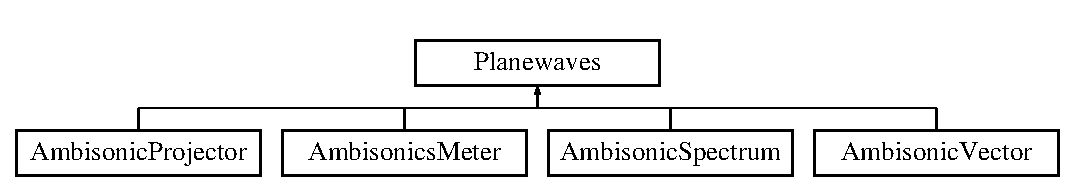
\includegraphics[height=1.709924cm]{class_planewaves}
\end{center}
\end{figure}
\subsection*{Public Member Functions}
\begin{DoxyCompactItemize}
\item 
\hyperlink{class_planewaves_ae42541fd2c6919293813f378ccb6e785}{Planewaves} (long a\-Number\-Of\-Loudspeakers=1, long a\-Vector\-Size=0, double a\-Sampling\-Rate=44100.)
\end{DoxyCompactItemize}


\subsection{Detailed Description}
Hoa\-Library \-: A High Order Ambisonics Library Copyright (c) 2012-\/2013 Julien Colafrancesco, Pierre Guillot, Eliott Paris, C\-I\-C\-M, Universite Paris-\/8. All rights reserved.\-re Guillot, C\-I\-C\-M -\/ Université Paris 8 All rights reserved.

Website \-: \href{http://www.mshparisnord.fr/HoaLibrary/}{\tt http\-://www.\-mshparisnord.\-fr/\-Hoa\-Library/} Contacts \-: \href{mailto:cicm.mshparisnord@gmail.com}{\tt cicm.\-mshparisnord@gmail.\-com}

This file is part of H\-O\-A L\-I\-B\-R\-A\-R\-Y.

H\-O\-A L\-I\-B\-R\-A\-R\-Y is free software\-: you can redistribute it and/or modify it under the terms of the G\-N\-U General Public License as published by the Free Software Foundation, either version 3 of the License, or (at your option) any later version.

This program is distributed in the hope that it will be useful, but W\-I\-T\-H\-O\-U\-T A\-N\-Y W\-A\-R\-R\-A\-N\-T\-Y; without even the implied warranty of M\-E\-R\-C\-H\-A\-N\-T\-A\-B\-I\-L\-I\-T\-Y or F\-I\-T\-N\-E\-S\-S F\-O\-R A P\-A\-R\-T\-I\-C\-U\-L\-A\-R P\-U\-R\-P\-O\-S\-E. See the G\-N\-U General Public License for more details.

You should have received a copy of the G\-N\-U General Public License along with this program. If not, see \href{http://www.gnu.org/licenses/}{\tt http\-://www.\-gnu.\-org/licenses/}. 

Definition at line 32 of file Planewaves.\-h.



\subsection{Constructor \& Destructor Documentation}
\hypertarget{class_planewaves_ae42541fd2c6919293813f378ccb6e785}{\index{Planewaves@{Planewaves}!Planewaves@{Planewaves}}
\index{Planewaves@{Planewaves}!Planewaves@{Planewaves}}
\subsubsection[{Planewaves}]{\setlength{\rightskip}{0pt plus 5cm}Planewaves\-::\-Planewaves (
\begin{DoxyParamCaption}
\item[{long}]{a\-Number\-Of\-Loudspeakers = {\ttfamily 1}, }
\item[{long}]{a\-Vector\-Size = {\ttfamily 0}, }
\item[{double}]{a\-Sampling\-Rate = {\ttfamily 44100.}}
\end{DoxyParamCaption}
)}}\label{class_planewaves_ae42541fd2c6919293813f378ccb6e785}
Hoa\-Library \-: A High Order Ambisonics Library Copyright (c) 2012-\/2013 Julien Colafrancesco, Pierre Guillot, Eliott Paris, C\-I\-C\-M, Universite Paris-\/8. All rights reserved.\-re Guillot, C\-I\-C\-M -\/ Université Paris 8 All rights reserved.

Website \-: \href{http://www.mshparisnord.fr/HoaLibrary/}{\tt http\-://www.\-mshparisnord.\-fr/\-Hoa\-Library/} Contacts \-: \href{mailto:cicm.mshparisnord@gmail.com}{\tt cicm.\-mshparisnord@gmail.\-com}

This file is part of H\-O\-A L\-I\-B\-R\-A\-R\-Y.

H\-O\-A L\-I\-B\-R\-A\-R\-Y is free software\-: you can redistribute it and/or modify it under the terms of the G\-N\-U General Public License as published by the Free Software Foundation, either version 3 of the License, or (at your option) any later version.

This program is distributed in the hope that it will be useful, but W\-I\-T\-H\-O\-U\-T A\-N\-Y W\-A\-R\-R\-A\-N\-T\-Y; without even the implied warranty of M\-E\-R\-C\-H\-A\-N\-T\-A\-B\-I\-L\-I\-T\-Y or F\-I\-T\-N\-E\-S\-S F\-O\-R A P\-A\-R\-T\-I\-C\-U\-L\-A\-R P\-U\-R\-P\-O\-S\-E. See the G\-N\-U General Public License for more details.

You should have received a copy of the G\-N\-U General Public License along with this program. If not, see \href{http://www.gnu.org/licenses/}{\tt http\-://www.\-gnu.\-org/licenses/}. 

Definition at line 29 of file Planewaves.\-cpp.



The documentation for this class was generated from the following files\-:\begin{DoxyCompactItemize}
\item 
/\-Users/\-Pierre/\-Source\-Tree/\-Hoa\-Library/\-Sources/hoa\-Ambisonics/Planewaves.\-h\item 
/\-Users/\-Pierre/\-Source\-Tree/\-Hoa\-Library/\-Sources/hoa\-Ambisonics/Planewaves.\-cpp\end{DoxyCompactItemize}

\hypertarget{struct_point2d}{\section{Point2d Struct Reference}
\label{struct_point2d}\index{Point2d@{Point2d}}
}
\subsection*{Public Attributes}
\begin{DoxyCompactItemize}
\item 
\hypertarget{struct_point2d_a410f46be7d944e2b4aae2c6ccfaae1b5}{double {\bfseries x}}\label{struct_point2d_a410f46be7d944e2b4aae2c6ccfaae1b5}

\item 
\hypertarget{struct_point2d_a39331cc20a1d3950122ab3845edb0689}{double {\bfseries y}}\label{struct_point2d_a39331cc20a1d3950122ab3845edb0689}

\end{DoxyCompactItemize}


The documentation for this struct was generated from the following file\-:\begin{DoxyCompactItemize}
\item 
/\-Users/\-Pierre/\-Source\-Tree/\-Hoa\-Library/\-Sources/hoa\-Boids/Boids\-Manager.\-h\end{DoxyCompactItemize}

\hypertarget{class_satellite}{\section{Satellite Class Reference}
\label{class_satellite}\index{Satellite@{Satellite}}
}


{\ttfamily \#include $<$Ambisonics\-Satellite.\-h$>$}

Inheritance diagram for Satellite\-:\begin{figure}[H]
\begin{center}
\leavevmode
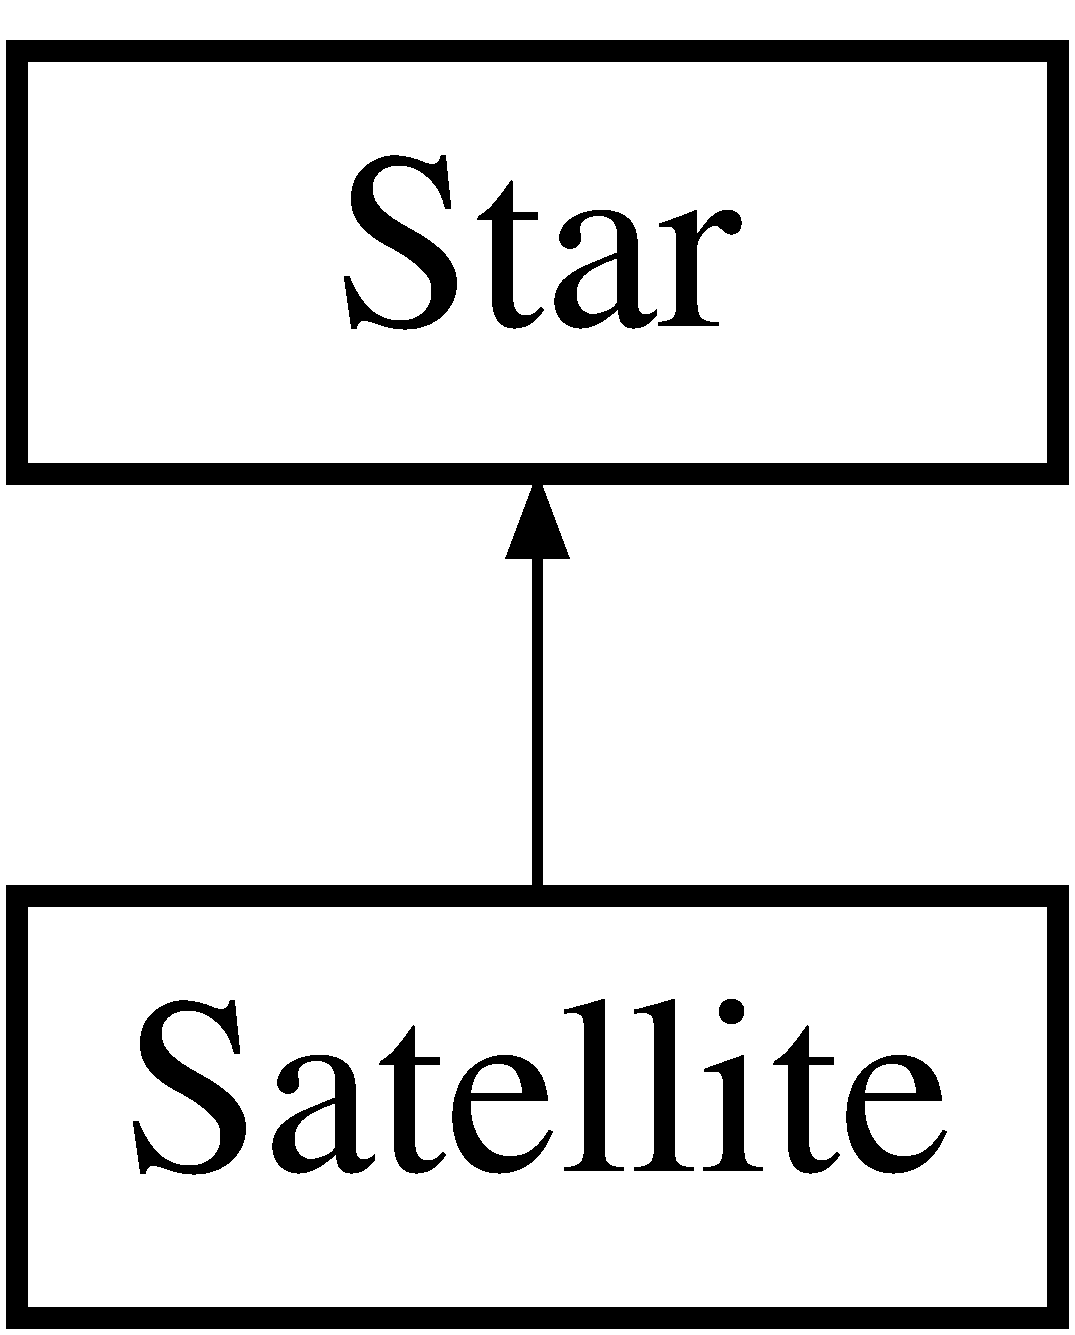
\includegraphics[height=2.000000cm]{class_satellite}
\end{center}
\end{figure}
\subsection*{Public Member Functions}
\begin{DoxyCompactItemize}
\item 
\hyperlink{class_satellite_ae33ea904e7f06940431573b906d19bed}{Satellite} (\hyperlink{class_star}{Star} $\ast$a\-Central\-Star, double an\-Elliptic\-Angle=0., double a\-Radius\-Principal=0., double a\-Radius\-Secondary=0.)
\end{DoxyCompactItemize}


\subsection{Detailed Description}
\hyperlink{interface_hoa_library}{Hoa\-Library} \-: A High Order Ambisonics Library Copyright (c) 2012-\/2013 Julien Colafrancesco, Pierre Guillot, Eliott Paris, C\-I\-C\-M, Universite Paris-\/8. All rights reserved.\-re Guillot, C\-I\-C\-M -\/ Université Paris 8 All rights reserved.

Website \-: \href{http://www.mshparisnord.fr/HoaLibrary/}{\tt http\-://www.\-mshparisnord.\-fr/\-Hoa\-Library/} Contacts \-: \href{mailto:cicm.mshparisnord@gmail.com}{\tt cicm.\-mshparisnord@gmail.\-com}

This file is part of H\-O\-A L\-I\-B\-R\-A\-R\-Y.

H\-O\-A L\-I\-B\-R\-A\-R\-Y is free software\-: you can redistribute it and/or modify it under the terms of the G\-N\-U General Public License as published by the Free Software Foundation, either version 3 of the License, or (at your option) any later version.

This program is distributed in the hope that it will be useful, but W\-I\-T\-H\-O\-U\-T A\-N\-Y W\-A\-R\-R\-A\-N\-T\-Y; without even the implied warranty of M\-E\-R\-C\-H\-A\-N\-T\-A\-B\-I\-L\-I\-T\-Y or F\-I\-T\-N\-E\-S\-S F\-O\-R A P\-A\-R\-T\-I\-C\-U\-L\-A\-R P\-U\-R\-P\-O\-S\-E. See the G\-N\-U General Public License for more details.

You should have received a copy of the G\-N\-U General Public License along with this program. If not, see \href{http://www.gnu.org/licenses/}{\tt http\-://www.\-gnu.\-org/licenses/}. 

Definition at line 33 of file Ambisonics\-Satellite.\-h.



\subsection{Constructor \& Destructor Documentation}
\hypertarget{class_satellite_ae33ea904e7f06940431573b906d19bed}{\index{Satellite@{Satellite}!Satellite@{Satellite}}
\index{Satellite@{Satellite}!Satellite@{Satellite}}
\subsubsection[{Satellite}]{\setlength{\rightskip}{0pt plus 5cm}Satellite\-::\-Satellite (
\begin{DoxyParamCaption}
\item[{{\bf Star} $\ast$}]{a\-Central\-Star, }
\item[{double}]{an\-Elliptic\-Angle = {\ttfamily 0.}, }
\item[{double}]{a\-Radius\-Principal = {\ttfamily 0.}, }
\item[{double}]{a\-Radius\-Secondary = {\ttfamily 0.}}
\end{DoxyParamCaption}
)}}\label{class_satellite_ae33ea904e7f06940431573b906d19bed}
\hyperlink{interface_hoa_library}{Hoa\-Library} \-: A High Order Ambisonics Library Copyright (c) 2012-\/2013 Julien Colafrancesco, Pierre Guillot, Eliott Paris, C\-I\-C\-M, Universite Paris-\/8. All rights reserved.\-re Guillot, C\-I\-C\-M -\/ Université Paris 8 All rights reserved.

Website \-: \href{http://www.mshparisnord.fr/HoaLibrary/}{\tt http\-://www.\-mshparisnord.\-fr/\-Hoa\-Library/} Contacts \-: \href{mailto:cicm.mshparisnord@gmail.com}{\tt cicm.\-mshparisnord@gmail.\-com}

This file is part of H\-O\-A L\-I\-B\-R\-A\-R\-Y.

H\-O\-A L\-I\-B\-R\-A\-R\-Y is free software\-: you can redistribute it and/or modify it under the terms of the G\-N\-U General Public License as published by the Free Software Foundation, either version 3 of the License, or (at your option) any later version.

This program is distributed in the hope that it will be useful, but W\-I\-T\-H\-O\-U\-T A\-N\-Y W\-A\-R\-R\-A\-N\-T\-Y; without even the implied warranty of M\-E\-R\-C\-H\-A\-N\-T\-A\-B\-I\-L\-I\-T\-Y or F\-I\-T\-N\-E\-S\-S F\-O\-R A P\-A\-R\-T\-I\-C\-U\-L\-A\-R P\-U\-R\-P\-O\-S\-E. See the G\-N\-U General Public License for more details.

You should have received a copy of the G\-N\-U General Public License along with this program. If not, see \href{http://www.gnu.org/licenses/}{\tt http\-://www.\-gnu.\-org/licenses/}. 

Definition at line 29 of file Ambisonics\-Satellite.\-cpp.



The documentation for this class was generated from the following files\-:\begin{DoxyCompactItemize}
\item 
/\-Users/\-Pierre/\-Source\-Tree/\-Hoa\-Library/\-Sources/hoa\-Galaxy/Ambisonics\-Satellite.\-h\item 
/\-Users/\-Pierre/\-Source\-Tree/\-Hoa\-Library/\-Sources/hoa\-Galaxy/Ambisonics\-Satellite.\-cpp\end{DoxyCompactItemize}

\hypertarget{class_sources_manager}{\section{Sources\-Manager Class Reference}
\label{class_sources_manager}\index{Sources\-Manager@{Sources\-Manager}}
}


{\ttfamily \#include $<$Ambisonic\-Sources\-Manager.\-h$>$}

\subsection*{Public Member Functions}
\begin{DoxyCompactItemize}
\item 
\hyperlink{class_sources_manager_a333ef82bab70b995bf0f658c894bee1b}{Sources\-Manager} (double a\-Maximum\-Limit\-Value=-\/1., long dead\-Or\-Alive=1)
\end{DoxyCompactItemize}


\subsection{Detailed Description}
\hyperlink{interface_hoa_library}{Hoa\-Library} \-: A High Order Ambisonics Library Copyright (c) 2012-\/2013 Julien Colafrancesco, Pierre Guillot, Eliott Paris, C\-I\-C\-M, Universite Paris-\/8. All rights reserved.

Website \-: \href{http://www.mshparisnord.fr/hoalibrary/}{\tt http\-://www.\-mshparisnord.\-fr/hoalibrary/} Contacts \-: \href{mailto:cicm.mshparisnord@gmail.com}{\tt cicm.\-mshparisnord@gmail.\-com}

Redistribution and use in source and binary forms, with or without modification, are permitted provided that the following conditions are met\-:


\begin{DoxyItemize}
\item Redistributions may not be sold, nor may they be used in a commercial product or activity.
\item Redistributions of source code must retain the above copyright notice, this list of conditions and the following disclaimer.
\item Redistributions in binary form must reproduce the above copyright notice, this list of conditions and the following disclaimer in the documentation and/or other materials provided with the distribution.
\item Neither the name of the C\-I\-C\-M nor the names of its contributors may be used to endorse or promote products derived from this software without specific prior written permission.
\end{DoxyItemize}

T\-H\-I\-S S\-O\-F\-T\-W\-A\-R\-E I\-S P\-R\-O\-V\-I\-D\-E\-D B\-Y T\-H\-E C\-O\-P\-Y\-R\-I\-G\-H\-T H\-O\-L\-D\-E\-R\-S A\-N\-D C\-O\-N\-T\-R\-I\-B\-U\-T\-O\-R\-S \char`\"{}\-A\-S I\-S\char`\"{} A\-N\-D A\-N\-Y E\-X\-P\-R\-E\-S\-S O\-R I\-M\-P\-L\-I\-E\-D W\-A\-R\-R\-A\-N\-T\-I\-E\-S, I\-N\-C\-L\-U\-D\-I\-N\-G, B\-U\-T N\-O\-T L\-I\-M\-I\-T\-E\-D T\-O, T\-H\-E I\-M\-P\-L\-I\-E\-D W\-A\-R\-R\-A\-N\-T\-I\-E\-S O\-F M\-E\-R\-C\-H\-A\-N\-T\-A\-B\-I\-L\-I\-T\-Y A\-N\-D F\-I\-T\-N\-E\-S\-S F\-O\-R A P\-A\-R\-T\-I\-C\-U\-L\-A\-R P\-U\-R\-P\-O\-S\-E A\-R\-E D\-I\-S\-C\-L\-A\-I\-M\-E\-D. I\-N N\-O E\-V\-E\-N\-T S\-H\-A\-L\-L T\-H\-E C\-O\-P\-Y\-R\-I\-G\-H\-T H\-O\-L\-D\-E\-R O\-R C\-O\-N\-T\-R\-I\-B\-U\-T\-O\-R\-S B\-E L\-I\-A\-B\-L\-E F\-O\-R A\-N\-Y D\-I\-R\-E\-C\-T, I\-N\-D\-I\-R\-E\-C\-T, I\-N\-C\-I\-D\-E\-N\-T\-A\-L, S\-P\-E\-C\-I\-A\-L, E\-X\-E\-M\-P\-L\-A\-R\-Y, O\-R C\-O\-N\-S\-E\-Q\-U\-E\-N\-T\-I\-A\-L D\-A\-M\-A\-G\-E\-S (I\-N\-C\-L\-U\-D\-I\-N\-G, B\-U\-T N\-O\-T L\-I\-M\-I\-T\-E\-D T\-O, P\-R\-O\-C\-U\-R\-E\-M\-E\-N\-T O\-F S\-U\-B\-S\-T\-I\-T\-U\-T\-E G\-O\-O\-D\-S O\-R S\-E\-R\-V\-I\-C\-E\-S; L\-O\-S\-S O\-F U\-S\-E, D\-A\-T\-A, O\-R P\-R\-O\-F\-I\-T\-S; O\-R B\-U\-S\-I\-N\-E\-S\-S I\-N\-T\-E\-R\-R\-U\-P\-T\-I\-O\-N) H\-O\-W\-E\-V\-E\-R C\-A\-U\-S\-E\-D A\-N\-D O\-N A\-N\-Y T\-H\-E\-O\-R\-Y O\-F L\-I\-A\-B\-I\-L\-I\-T\-Y, W\-H\-E\-T\-H\-E\-R I\-N C\-O\-N\-T\-R\-A\-C\-T, S\-T\-R\-I\-C\-T L\-I\-A\-B\-I\-L\-I\-T\-Y, O\-R T\-O\-R\-T (I\-N\-C\-L\-U\-D\-I\-N\-G N\-E\-G\-L\-I\-G\-E\-N\-C\-E O\-R O\-T\-H\-E\-R\-W\-I\-S\-E) A\-R\-I\-S\-I\-N\-G I\-N A\-N\-Y W\-A\-Y O\-U\-T O\-F T\-H\-E U\-S\-E O\-F T\-H\-I\-S S\-O\-F\-T\-W\-A\-R\-E, E\-V\-E\-N I\-F A\-D\-V\-I\-S\-E\-D O\-F T\-H\-E P\-O\-S\-S\-I\-B\-I\-L\-I\-T\-Y O\-F S\-U\-C\-H D\-A\-M\-A\-G\-E. 

Definition at line 32 of file Ambisonic\-Sources\-Manager.\-h.



\subsection{Constructor \& Destructor Documentation}
\hypertarget{class_sources_manager_a333ef82bab70b995bf0f658c894bee1b}{\index{Sources\-Manager@{Sources\-Manager}!Sources\-Manager@{Sources\-Manager}}
\index{Sources\-Manager@{Sources\-Manager}!SourcesManager@{Sources\-Manager}}
\subsubsection[{Sources\-Manager}]{\setlength{\rightskip}{0pt plus 5cm}Sources\-Manager\-::\-Sources\-Manager (
\begin{DoxyParamCaption}
\item[{double}]{a\-Maximum\-Limit\-Value = {\ttfamily -\/1.}, }
\item[{long}]{dead\-Or\-Alive = {\ttfamily 1}}
\end{DoxyParamCaption}
)}}\label{class_sources_manager_a333ef82bab70b995bf0f658c894bee1b}
\hyperlink{interface_hoa_library}{Hoa\-Library} \-: A High Order Ambisonics Library Copyright (c) 2012-\/2013 Julien Colafrancesco, Pierre Guillot, Eliott Paris, C\-I\-C\-M, Universite Paris-\/8. All rights reserved.

Website \-: \href{http://www.mshparisnord.fr/hoalibrary/}{\tt http\-://www.\-mshparisnord.\-fr/hoalibrary/} Contacts \-: \href{mailto:cicm.mshparisnord@gmail.com}{\tt cicm.\-mshparisnord@gmail.\-com}

Redistribution and use in source and binary forms, with or without modification, are permitted provided that the following conditions are met\-:


\begin{DoxyItemize}
\item Redistributions may not be sold, nor may they be used in a commercial product or activity.
\item Redistributions of source code must retain the above copyright notice, this list of conditions and the following disclaimer.
\item Redistributions in binary form must reproduce the above copyright notice, this list of conditions and the following disclaimer in the documentation and/or other materials provided with the distribution.
\item Neither the name of the C\-I\-C\-M nor the names of its contributors may be used to endorse or promote products derived from this software without specific prior written permission.
\end{DoxyItemize}

T\-H\-I\-S S\-O\-F\-T\-W\-A\-R\-E I\-S P\-R\-O\-V\-I\-D\-E\-D B\-Y T\-H\-E C\-O\-P\-Y\-R\-I\-G\-H\-T H\-O\-L\-D\-E\-R\-S A\-N\-D C\-O\-N\-T\-R\-I\-B\-U\-T\-O\-R\-S \char`\"{}\-A\-S I\-S\char`\"{} A\-N\-D A\-N\-Y E\-X\-P\-R\-E\-S\-S O\-R I\-M\-P\-L\-I\-E\-D W\-A\-R\-R\-A\-N\-T\-I\-E\-S, I\-N\-C\-L\-U\-D\-I\-N\-G, B\-U\-T N\-O\-T L\-I\-M\-I\-T\-E\-D T\-O, T\-H\-E I\-M\-P\-L\-I\-E\-D W\-A\-R\-R\-A\-N\-T\-I\-E\-S O\-F M\-E\-R\-C\-H\-A\-N\-T\-A\-B\-I\-L\-I\-T\-Y A\-N\-D F\-I\-T\-N\-E\-S\-S F\-O\-R A P\-A\-R\-T\-I\-C\-U\-L\-A\-R P\-U\-R\-P\-O\-S\-E A\-R\-E D\-I\-S\-C\-L\-A\-I\-M\-E\-D. I\-N N\-O E\-V\-E\-N\-T S\-H\-A\-L\-L T\-H\-E C\-O\-P\-Y\-R\-I\-G\-H\-T H\-O\-L\-D\-E\-R O\-R C\-O\-N\-T\-R\-I\-B\-U\-T\-O\-R\-S B\-E L\-I\-A\-B\-L\-E F\-O\-R A\-N\-Y D\-I\-R\-E\-C\-T, I\-N\-D\-I\-R\-E\-C\-T, I\-N\-C\-I\-D\-E\-N\-T\-A\-L, S\-P\-E\-C\-I\-A\-L, E\-X\-E\-M\-P\-L\-A\-R\-Y, O\-R C\-O\-N\-S\-E\-Q\-U\-E\-N\-T\-I\-A\-L D\-A\-M\-A\-G\-E\-S (I\-N\-C\-L\-U\-D\-I\-N\-G, B\-U\-T N\-O\-T L\-I\-M\-I\-T\-E\-D T\-O, P\-R\-O\-C\-U\-R\-E\-M\-E\-N\-T O\-F S\-U\-B\-S\-T\-I\-T\-U\-T\-E G\-O\-O\-D\-S O\-R S\-E\-R\-V\-I\-C\-E\-S; L\-O\-S\-S O\-F U\-S\-E, D\-A\-T\-A, O\-R P\-R\-O\-F\-I\-T\-S; O\-R B\-U\-S\-I\-N\-E\-S\-S I\-N\-T\-E\-R\-R\-U\-P\-T\-I\-O\-N) H\-O\-W\-E\-V\-E\-R C\-A\-U\-S\-E\-D A\-N\-D O\-N A\-N\-Y T\-H\-E\-O\-R\-Y O\-F L\-I\-A\-B\-I\-L\-I\-T\-Y, W\-H\-E\-T\-H\-E\-R I\-N C\-O\-N\-T\-R\-A\-C\-T, S\-T\-R\-I\-C\-T L\-I\-A\-B\-I\-L\-I\-T\-Y, O\-R T\-O\-R\-T (I\-N\-C\-L\-U\-D\-I\-N\-G N\-E\-G\-L\-I\-G\-E\-N\-C\-E O\-R O\-T\-H\-E\-R\-W\-I\-S\-E) A\-R\-I\-S\-I\-N\-G I\-N A\-N\-Y W\-A\-Y O\-U\-T O\-F T\-H\-E U\-S\-E O\-F T\-H\-I\-S S\-O\-F\-T\-W\-A\-R\-E, E\-V\-E\-N I\-F A\-D\-V\-I\-S\-E\-D O\-F T\-H\-E P\-O\-S\-S\-I\-B\-I\-L\-I\-T\-Y O\-F S\-U\-C\-H D\-A\-M\-A\-G\-E. 

Definition at line 28 of file Ambisonic\-Sources\-Manager.\-cpp.



The documentation for this class was generated from the following files\-:\begin{DoxyCompactItemize}
\item 
/\-Users/\-Pierre/\-Source\-Tree/\-Hoa\-Library/\-Sources/hoa\-Map/Ambisonic\-Sources\-Manager.\-h\item 
/\-Users/\-Pierre/\-Source\-Tree/\-Hoa\-Library/\-Sources/hoa\-Map/Ambisonic\-Sources\-Manager.\-cpp\end{DoxyCompactItemize}

\hypertarget{class_sources_preset}{\section{Sources\-Preset Class Reference}
\label{class_sources_preset}\index{Sources\-Preset@{Sources\-Preset}}
}


{\ttfamily \#include $<$Ambisonic\-Sources\-Preset.\-h$>$}

Inheritance diagram for Sources\-Preset\-:\begin{figure}[H]
\begin{center}
\leavevmode
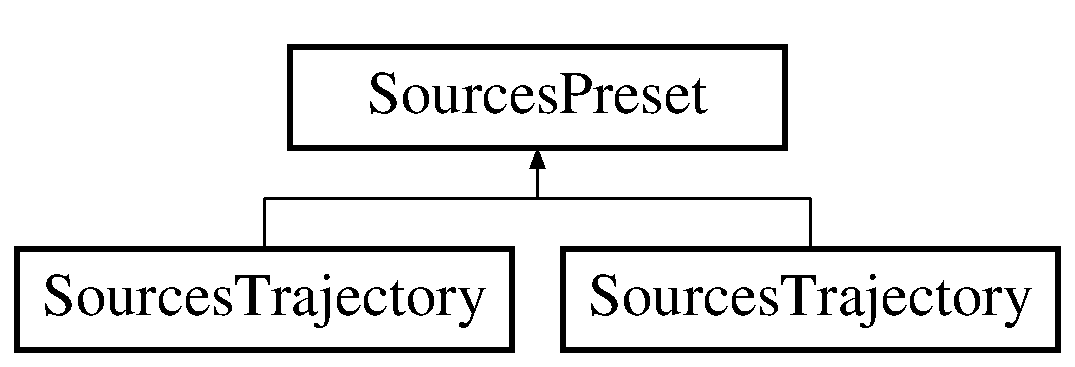
\includegraphics[height=2.000000cm]{class_sources_preset}
\end{center}
\end{figure}
\subsection*{Public Member Functions}
\begin{DoxyCompactItemize}
\item 
\hyperlink{class_sources_preset_a0a4203349327d10bb6afe35156126d8a}{Sources\-Preset} ()
\end{DoxyCompactItemize}


\subsection{Detailed Description}
Hoa\-Library \-: A High Order Ambisonics Library Copyright (c) 2012-\/2013 Julien Colafrancesco, Pierre Guillot, Eliott Paris, C\-I\-C\-M, Universite Paris-\/8. All rights reserved.

Website \-: \href{http://www.mshparisnord.fr/hoalibrary/}{\tt http\-://www.\-mshparisnord.\-fr/hoalibrary/} Contacts \-: \href{mailto:cicm.mshparisnord@gmail.com}{\tt cicm.\-mshparisnord@gmail.\-com}

Redistribution and use in source and binary forms, with or without modification, are permitted provided that the following conditions are met\-:


\begin{DoxyItemize}
\item Redistributions may not be sold, nor may they be used in a commercial product or activity.
\item Redistributions of source code must retain the above copyright notice, this list of conditions and the following disclaimer.
\item Redistributions in binary form must reproduce the above copyright notice, this list of conditions and the following disclaimer in the documentation and/or other materials provided with the distribution.
\item Neither the name of the C\-I\-C\-M nor the names of its contributors may be used to endorse or promote products derived from this software without specific prior written permission.
\end{DoxyItemize}

T\-H\-I\-S S\-O\-F\-T\-W\-A\-R\-E I\-S P\-R\-O\-V\-I\-D\-E\-D B\-Y T\-H\-E C\-O\-P\-Y\-R\-I\-G\-H\-T H\-O\-L\-D\-E\-R\-S A\-N\-D C\-O\-N\-T\-R\-I\-B\-U\-T\-O\-R\-S \char`\"{}\-A\-S I\-S\char`\"{} A\-N\-D A\-N\-Y E\-X\-P\-R\-E\-S\-S O\-R I\-M\-P\-L\-I\-E\-D W\-A\-R\-R\-A\-N\-T\-I\-E\-S, I\-N\-C\-L\-U\-D\-I\-N\-G, B\-U\-T N\-O\-T L\-I\-M\-I\-T\-E\-D T\-O, T\-H\-E I\-M\-P\-L\-I\-E\-D W\-A\-R\-R\-A\-N\-T\-I\-E\-S O\-F M\-E\-R\-C\-H\-A\-N\-T\-A\-B\-I\-L\-I\-T\-Y A\-N\-D F\-I\-T\-N\-E\-S\-S F\-O\-R A P\-A\-R\-T\-I\-C\-U\-L\-A\-R P\-U\-R\-P\-O\-S\-E A\-R\-E D\-I\-S\-C\-L\-A\-I\-M\-E\-D. I\-N N\-O E\-V\-E\-N\-T S\-H\-A\-L\-L T\-H\-E C\-O\-P\-Y\-R\-I\-G\-H\-T H\-O\-L\-D\-E\-R O\-R C\-O\-N\-T\-R\-I\-B\-U\-T\-O\-R\-S B\-E L\-I\-A\-B\-L\-E F\-O\-R A\-N\-Y D\-I\-R\-E\-C\-T, I\-N\-D\-I\-R\-E\-C\-T, I\-N\-C\-I\-D\-E\-N\-T\-A\-L, S\-P\-E\-C\-I\-A\-L, E\-X\-E\-M\-P\-L\-A\-R\-Y, O\-R C\-O\-N\-S\-E\-Q\-U\-E\-N\-T\-I\-A\-L D\-A\-M\-A\-G\-E\-S (I\-N\-C\-L\-U\-D\-I\-N\-G, B\-U\-T N\-O\-T L\-I\-M\-I\-T\-E\-D T\-O, P\-R\-O\-C\-U\-R\-E\-M\-E\-N\-T O\-F S\-U\-B\-S\-T\-I\-T\-U\-T\-E G\-O\-O\-D\-S O\-R S\-E\-R\-V\-I\-C\-E\-S; L\-O\-S\-S O\-F U\-S\-E, D\-A\-T\-A, O\-R P\-R\-O\-F\-I\-T\-S; O\-R B\-U\-S\-I\-N\-E\-S\-S I\-N\-T\-E\-R\-R\-U\-P\-T\-I\-O\-N) H\-O\-W\-E\-V\-E\-R C\-A\-U\-S\-E\-D A\-N\-D O\-N A\-N\-Y T\-H\-E\-O\-R\-Y O\-F L\-I\-A\-B\-I\-L\-I\-T\-Y, W\-H\-E\-T\-H\-E\-R I\-N C\-O\-N\-T\-R\-A\-C\-T, S\-T\-R\-I\-C\-T L\-I\-A\-B\-I\-L\-I\-T\-Y, O\-R T\-O\-R\-T (I\-N\-C\-L\-U\-D\-I\-N\-G N\-E\-G\-L\-I\-G\-E\-N\-C\-E O\-R O\-T\-H\-E\-R\-W\-I\-S\-E) A\-R\-I\-S\-I\-N\-G I\-N A\-N\-Y W\-A\-Y O\-U\-T O\-F T\-H\-E U\-S\-E O\-F T\-H\-I\-S S\-O\-F\-T\-W\-A\-R\-E, E\-V\-E\-N I\-F A\-D\-V\-I\-S\-E\-D O\-F T\-H\-E P\-O\-S\-S\-I\-B\-I\-L\-I\-T\-Y O\-F S\-U\-C\-H D\-A\-M\-A\-G\-E. 

Definition at line 31 of file Ambisonic\-Sources\-Preset.\-h.



\subsection{Constructor \& Destructor Documentation}
\hypertarget{class_sources_preset_a0a4203349327d10bb6afe35156126d8a}{\index{Sources\-Preset@{Sources\-Preset}!Sources\-Preset@{Sources\-Preset}}
\index{Sources\-Preset@{Sources\-Preset}!SourcesPreset@{Sources\-Preset}}
\subsubsection[{Sources\-Preset}]{\setlength{\rightskip}{0pt plus 5cm}Sources\-Preset\-::\-Sources\-Preset (
\begin{DoxyParamCaption}
{}
\end{DoxyParamCaption}
)}}\label{class_sources_preset_a0a4203349327d10bb6afe35156126d8a}
Hoa\-Library \-: A High Order Ambisonics Library Copyright (c) 2012-\/2013 Julien Colafrancesco, Pierre Guillot, Eliott Paris, C\-I\-C\-M, Universite Paris-\/8. All rights reserved.

Website \-: \href{http://www.mshparisnord.fr/hoalibrary/}{\tt http\-://www.\-mshparisnord.\-fr/hoalibrary/} Contacts \-: \href{mailto:cicm.mshparisnord@gmail.com}{\tt cicm.\-mshparisnord@gmail.\-com}

Redistribution and use in source and binary forms, with or without modification, are permitted provided that the following conditions are met\-:


\begin{DoxyItemize}
\item Redistributions may not be sold, nor may they be used in a commercial product or activity.
\item Redistributions of source code must retain the above copyright notice, this list of conditions and the following disclaimer.
\item Redistributions in binary form must reproduce the above copyright notice, this list of conditions and the following disclaimer in the documentation and/or other materials provided with the distribution.
\item Neither the name of the C\-I\-C\-M nor the names of its contributors may be used to endorse or promote products derived from this software without specific prior written permission.
\end{DoxyItemize}

T\-H\-I\-S S\-O\-F\-T\-W\-A\-R\-E I\-S P\-R\-O\-V\-I\-D\-E\-D B\-Y T\-H\-E C\-O\-P\-Y\-R\-I\-G\-H\-T H\-O\-L\-D\-E\-R\-S A\-N\-D C\-O\-N\-T\-R\-I\-B\-U\-T\-O\-R\-S \char`\"{}\-A\-S I\-S\char`\"{} A\-N\-D A\-N\-Y E\-X\-P\-R\-E\-S\-S O\-R I\-M\-P\-L\-I\-E\-D W\-A\-R\-R\-A\-N\-T\-I\-E\-S, I\-N\-C\-L\-U\-D\-I\-N\-G, B\-U\-T N\-O\-T L\-I\-M\-I\-T\-E\-D T\-O, T\-H\-E I\-M\-P\-L\-I\-E\-D W\-A\-R\-R\-A\-N\-T\-I\-E\-S O\-F M\-E\-R\-C\-H\-A\-N\-T\-A\-B\-I\-L\-I\-T\-Y A\-N\-D F\-I\-T\-N\-E\-S\-S F\-O\-R A P\-A\-R\-T\-I\-C\-U\-L\-A\-R P\-U\-R\-P\-O\-S\-E A\-R\-E D\-I\-S\-C\-L\-A\-I\-M\-E\-D. I\-N N\-O E\-V\-E\-N\-T S\-H\-A\-L\-L T\-H\-E C\-O\-P\-Y\-R\-I\-G\-H\-T H\-O\-L\-D\-E\-R O\-R C\-O\-N\-T\-R\-I\-B\-U\-T\-O\-R\-S B\-E L\-I\-A\-B\-L\-E F\-O\-R A\-N\-Y D\-I\-R\-E\-C\-T, I\-N\-D\-I\-R\-E\-C\-T, I\-N\-C\-I\-D\-E\-N\-T\-A\-L, S\-P\-E\-C\-I\-A\-L, E\-X\-E\-M\-P\-L\-A\-R\-Y, O\-R C\-O\-N\-S\-E\-Q\-U\-E\-N\-T\-I\-A\-L D\-A\-M\-A\-G\-E\-S (I\-N\-C\-L\-U\-D\-I\-N\-G, B\-U\-T N\-O\-T L\-I\-M\-I\-T\-E\-D T\-O, P\-R\-O\-C\-U\-R\-E\-M\-E\-N\-T O\-F S\-U\-B\-S\-T\-I\-T\-U\-T\-E G\-O\-O\-D\-S O\-R S\-E\-R\-V\-I\-C\-E\-S; L\-O\-S\-S O\-F U\-S\-E, D\-A\-T\-A, O\-R P\-R\-O\-F\-I\-T\-S; O\-R B\-U\-S\-I\-N\-E\-S\-S I\-N\-T\-E\-R\-R\-U\-P\-T\-I\-O\-N) H\-O\-W\-E\-V\-E\-R C\-A\-U\-S\-E\-D A\-N\-D O\-N A\-N\-Y T\-H\-E\-O\-R\-Y O\-F L\-I\-A\-B\-I\-L\-I\-T\-Y, W\-H\-E\-T\-H\-E\-R I\-N C\-O\-N\-T\-R\-A\-C\-T, S\-T\-R\-I\-C\-T L\-I\-A\-B\-I\-L\-I\-T\-Y, O\-R T\-O\-R\-T (I\-N\-C\-L\-U\-D\-I\-N\-G N\-E\-G\-L\-I\-G\-E\-N\-C\-E O\-R O\-T\-H\-E\-R\-W\-I\-S\-E) A\-R\-I\-S\-I\-N\-G I\-N A\-N\-Y W\-A\-Y O\-U\-T O\-F T\-H\-E U\-S\-E O\-F T\-H\-I\-S S\-O\-F\-T\-W\-A\-R\-E, E\-V\-E\-N I\-F A\-D\-V\-I\-S\-E\-D O\-F T\-H\-E P\-O\-S\-S\-I\-B\-I\-L\-I\-T\-Y O\-F S\-U\-C\-H D\-A\-M\-A\-G\-E. 

Definition at line 28 of file Ambisonic\-Sources\-Preset.\-cpp.



The documentation for this class was generated from the following files\-:\begin{DoxyCompactItemize}
\item 
/\-Users/elioton/\-Documents/programmation/\-C\-I\-C\-M/source\-Tree/\-Hoa\-Library/\-Sources/hoa\-Map/Ambisonic\-Sources\-Preset.\-h\item 
/\-Users/elioton/\-Documents/programmation/\-C\-I\-C\-M/source\-Tree/\-Hoa\-Library/\-Sources/hoa\-Map/Ambisonic\-Sources\-Preset.\-cpp\end{DoxyCompactItemize}

\hypertarget{class_sources_trajectory}{\section{Sources\-Trajectory Class Reference}
\label{class_sources_trajectory}\index{Sources\-Trajectory@{Sources\-Trajectory}}
}


{\ttfamily \#include $<$Ambisonic\-Sources\-Trajectory.\-h$>$}

Inheritance diagram for Sources\-Trajectory\-:\begin{figure}[H]
\begin{center}
\leavevmode
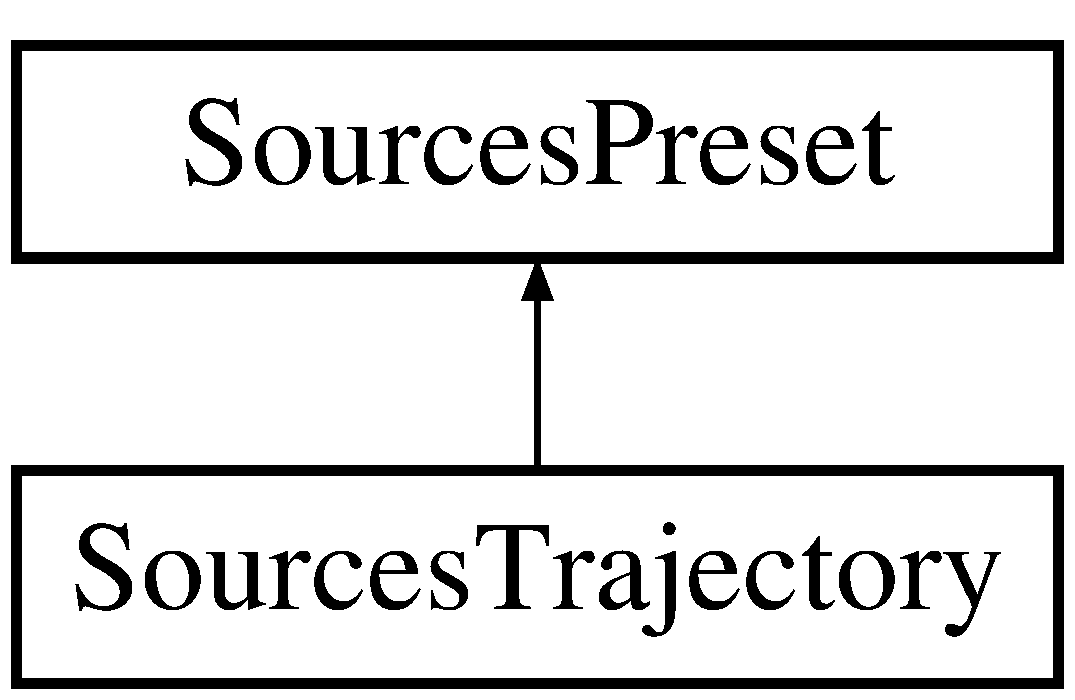
\includegraphics[height=2.000000cm]{class_sources_trajectory}
\end{center}
\end{figure}
\subsection*{Public Member Functions}
\begin{DoxyCompactItemize}
\item 
\hyperlink{class_sources_trajectory_a6e0838cc0ab29b5462cc624958498c4d}{Sources\-Trajectory} ()
\end{DoxyCompactItemize}


\subsection{Detailed Description}
Hoa\-Library \-: A High Order Ambisonics Library Copyright (c) 2012-\/2013 Julien Colafrancesco, Pierre Guillot, Eliott Paris, C\-I\-C\-M, Universite Paris-\/8. All rights reserved.

Website \-: \href{http://www.mshparisnord.fr/hoalibrary/}{\tt http\-://www.\-mshparisnord.\-fr/hoalibrary/} Contacts \-: \href{mailto:cicm.mshparisnord@gmail.com}{\tt cicm.\-mshparisnord@gmail.\-com}

Redistribution and use in source and binary forms, with or without modification, are permitted provided that the following conditions are met\-:


\begin{DoxyItemize}
\item Redistributions may not be sold, nor may they be used in a commercial product or activity.
\item Redistributions of source code must retain the above copyright notice, this list of conditions and the following disclaimer.
\item Redistributions in binary form must reproduce the above copyright notice, this list of conditions and the following disclaimer in the documentation and/or other materials provided with the distribution.
\item Neither the name of the C\-I\-C\-M nor the names of its contributors may be used to endorse or promote products derived from this software without specific prior written permission.
\end{DoxyItemize}

T\-H\-I\-S S\-O\-F\-T\-W\-A\-R\-E I\-S P\-R\-O\-V\-I\-D\-E\-D B\-Y T\-H\-E C\-O\-P\-Y\-R\-I\-G\-H\-T H\-O\-L\-D\-E\-R\-S A\-N\-D C\-O\-N\-T\-R\-I\-B\-U\-T\-O\-R\-S \char`\"{}\-A\-S I\-S\char`\"{} A\-N\-D A\-N\-Y E\-X\-P\-R\-E\-S\-S O\-R I\-M\-P\-L\-I\-E\-D W\-A\-R\-R\-A\-N\-T\-I\-E\-S, I\-N\-C\-L\-U\-D\-I\-N\-G, B\-U\-T N\-O\-T L\-I\-M\-I\-T\-E\-D T\-O, T\-H\-E I\-M\-P\-L\-I\-E\-D W\-A\-R\-R\-A\-N\-T\-I\-E\-S O\-F M\-E\-R\-C\-H\-A\-N\-T\-A\-B\-I\-L\-I\-T\-Y A\-N\-D F\-I\-T\-N\-E\-S\-S F\-O\-R A P\-A\-R\-T\-I\-C\-U\-L\-A\-R P\-U\-R\-P\-O\-S\-E A\-R\-E D\-I\-S\-C\-L\-A\-I\-M\-E\-D. I\-N N\-O E\-V\-E\-N\-T S\-H\-A\-L\-L T\-H\-E C\-O\-P\-Y\-R\-I\-G\-H\-T H\-O\-L\-D\-E\-R O\-R C\-O\-N\-T\-R\-I\-B\-U\-T\-O\-R\-S B\-E L\-I\-A\-B\-L\-E F\-O\-R A\-N\-Y D\-I\-R\-E\-C\-T, I\-N\-D\-I\-R\-E\-C\-T, I\-N\-C\-I\-D\-E\-N\-T\-A\-L, S\-P\-E\-C\-I\-A\-L, E\-X\-E\-M\-P\-L\-A\-R\-Y, O\-R C\-O\-N\-S\-E\-Q\-U\-E\-N\-T\-I\-A\-L D\-A\-M\-A\-G\-E\-S (I\-N\-C\-L\-U\-D\-I\-N\-G, B\-U\-T N\-O\-T L\-I\-M\-I\-T\-E\-D T\-O, P\-R\-O\-C\-U\-R\-E\-M\-E\-N\-T O\-F S\-U\-B\-S\-T\-I\-T\-U\-T\-E G\-O\-O\-D\-S O\-R S\-E\-R\-V\-I\-C\-E\-S; L\-O\-S\-S O\-F U\-S\-E, D\-A\-T\-A, O\-R P\-R\-O\-F\-I\-T\-S; O\-R B\-U\-S\-I\-N\-E\-S\-S I\-N\-T\-E\-R\-R\-U\-P\-T\-I\-O\-N) H\-O\-W\-E\-V\-E\-R C\-A\-U\-S\-E\-D A\-N\-D O\-N A\-N\-Y T\-H\-E\-O\-R\-Y O\-F L\-I\-A\-B\-I\-L\-I\-T\-Y, W\-H\-E\-T\-H\-E\-R I\-N C\-O\-N\-T\-R\-A\-C\-T, S\-T\-R\-I\-C\-T L\-I\-A\-B\-I\-L\-I\-T\-Y, O\-R T\-O\-R\-T (I\-N\-C\-L\-U\-D\-I\-N\-G N\-E\-G\-L\-I\-G\-E\-N\-C\-E O\-R O\-T\-H\-E\-R\-W\-I\-S\-E) A\-R\-I\-S\-I\-N\-G I\-N A\-N\-Y W\-A\-Y O\-U\-T O\-F T\-H\-E U\-S\-E O\-F T\-H\-I\-S S\-O\-F\-T\-W\-A\-R\-E, E\-V\-E\-N I\-F A\-D\-V\-I\-S\-E\-D O\-F T\-H\-E P\-O\-S\-S\-I\-B\-I\-L\-I\-T\-Y O\-F S\-U\-C\-H D\-A\-M\-A\-G\-E. 

Definition at line 31 of file Ambisonic\-Sources\-Trajectory.\-h.



\subsection{Constructor \& Destructor Documentation}
\hypertarget{class_sources_trajectory_a6e0838cc0ab29b5462cc624958498c4d}{\index{Sources\-Trajectory@{Sources\-Trajectory}!Sources\-Trajectory@{Sources\-Trajectory}}
\index{Sources\-Trajectory@{Sources\-Trajectory}!SourcesTrajectory@{Sources\-Trajectory}}
\subsubsection[{Sources\-Trajectory}]{\setlength{\rightskip}{0pt plus 5cm}Sources\-Trajectory\-::\-Sources\-Trajectory (
\begin{DoxyParamCaption}
{}
\end{DoxyParamCaption}
)}}\label{class_sources_trajectory_a6e0838cc0ab29b5462cc624958498c4d}
Hoa\-Library \-: A High Order Ambisonics Library Copyright (c) 2012-\/2013 Julien Colafrancesco, Pierre Guillot, Eliott Paris, C\-I\-C\-M, Universite Paris-\/8. All rights reserved.

Website \-: \href{http://www.mshparisnord.fr/hoalibrary/}{\tt http\-://www.\-mshparisnord.\-fr/hoalibrary/} Contacts \-: \href{mailto:cicm.mshparisnord@gmail.com}{\tt cicm.\-mshparisnord@gmail.\-com}

Redistribution and use in source and binary forms, with or without modification, are permitted provided that the following conditions are met\-:


\begin{DoxyItemize}
\item Redistributions may not be sold, nor may they be used in a commercial product or activity.
\item Redistributions of source code must retain the above copyright notice, this list of conditions and the following disclaimer.
\item Redistributions in binary form must reproduce the above copyright notice, this list of conditions and the following disclaimer in the documentation and/or other materials provided with the distribution.
\item Neither the name of the C\-I\-C\-M nor the names of its contributors may be used to endorse or promote products derived from this software without specific prior written permission.
\end{DoxyItemize}

T\-H\-I\-S S\-O\-F\-T\-W\-A\-R\-E I\-S P\-R\-O\-V\-I\-D\-E\-D B\-Y T\-H\-E C\-O\-P\-Y\-R\-I\-G\-H\-T H\-O\-L\-D\-E\-R\-S A\-N\-D C\-O\-N\-T\-R\-I\-B\-U\-T\-O\-R\-S \char`\"{}\-A\-S I\-S\char`\"{} A\-N\-D A\-N\-Y E\-X\-P\-R\-E\-S\-S O\-R I\-M\-P\-L\-I\-E\-D W\-A\-R\-R\-A\-N\-T\-I\-E\-S, I\-N\-C\-L\-U\-D\-I\-N\-G, B\-U\-T N\-O\-T L\-I\-M\-I\-T\-E\-D T\-O, T\-H\-E I\-M\-P\-L\-I\-E\-D W\-A\-R\-R\-A\-N\-T\-I\-E\-S O\-F M\-E\-R\-C\-H\-A\-N\-T\-A\-B\-I\-L\-I\-T\-Y A\-N\-D F\-I\-T\-N\-E\-S\-S F\-O\-R A P\-A\-R\-T\-I\-C\-U\-L\-A\-R P\-U\-R\-P\-O\-S\-E A\-R\-E D\-I\-S\-C\-L\-A\-I\-M\-E\-D. I\-N N\-O E\-V\-E\-N\-T S\-H\-A\-L\-L T\-H\-E C\-O\-P\-Y\-R\-I\-G\-H\-T H\-O\-L\-D\-E\-R O\-R C\-O\-N\-T\-R\-I\-B\-U\-T\-O\-R\-S B\-E L\-I\-A\-B\-L\-E F\-O\-R A\-N\-Y D\-I\-R\-E\-C\-T, I\-N\-D\-I\-R\-E\-C\-T, I\-N\-C\-I\-D\-E\-N\-T\-A\-L, S\-P\-E\-C\-I\-A\-L, E\-X\-E\-M\-P\-L\-A\-R\-Y, O\-R C\-O\-N\-S\-E\-Q\-U\-E\-N\-T\-I\-A\-L D\-A\-M\-A\-G\-E\-S (I\-N\-C\-L\-U\-D\-I\-N\-G, B\-U\-T N\-O\-T L\-I\-M\-I\-T\-E\-D T\-O, P\-R\-O\-C\-U\-R\-E\-M\-E\-N\-T O\-F S\-U\-B\-S\-T\-I\-T\-U\-T\-E G\-O\-O\-D\-S O\-R S\-E\-R\-V\-I\-C\-E\-S; L\-O\-S\-S O\-F U\-S\-E, D\-A\-T\-A, O\-R P\-R\-O\-F\-I\-T\-S; O\-R B\-U\-S\-I\-N\-E\-S\-S I\-N\-T\-E\-R\-R\-U\-P\-T\-I\-O\-N) H\-O\-W\-E\-V\-E\-R C\-A\-U\-S\-E\-D A\-N\-D O\-N A\-N\-Y T\-H\-E\-O\-R\-Y O\-F L\-I\-A\-B\-I\-L\-I\-T\-Y, W\-H\-E\-T\-H\-E\-R I\-N C\-O\-N\-T\-R\-A\-C\-T, S\-T\-R\-I\-C\-T L\-I\-A\-B\-I\-L\-I\-T\-Y, O\-R T\-O\-R\-T (I\-N\-C\-L\-U\-D\-I\-N\-G N\-E\-G\-L\-I\-G\-E\-N\-C\-E O\-R O\-T\-H\-E\-R\-W\-I\-S\-E) A\-R\-I\-S\-I\-N\-G I\-N A\-N\-Y W\-A\-Y O\-U\-T O\-F T\-H\-E U\-S\-E O\-F T\-H\-I\-S S\-O\-F\-T\-W\-A\-R\-E, E\-V\-E\-N I\-F A\-D\-V\-I\-S\-E\-D O\-F T\-H\-E P\-O\-S\-S\-I\-B\-I\-L\-I\-T\-Y O\-F S\-U\-C\-H D\-A\-M\-A\-G\-E. 

Definition at line 28 of file Ambisonic\-Sources\-Trajectory.\-cpp.



The documentation for this class was generated from the following files\-:\begin{DoxyCompactItemize}
\item 
/\-Users/elioton/\-Documents/programmation/\-C\-I\-C\-M/source\-Tree/\-Hoa\-Library/\-Sources/hoa\-Map/Ambisonic\-Sources\-Trajectory.\-h\item 
/\-Users/elioton/\-Documents/programmation/\-C\-I\-C\-M/source\-Tree/\-Hoa\-Library/\-Sources/hoa\-Map/Ambisonic\-Sources\-Trajectory.\-cpp\end{DoxyCompactItemize}

\hypertarget{class_star}{\section{Star Class Reference}
\label{class_star}\index{Star@{Star}}
}


{\ttfamily \#include $<$Ambisonics\-Star.\-h$>$}

Inheritance diagram for Star\-:\begin{figure}[H]
\begin{center}
\leavevmode
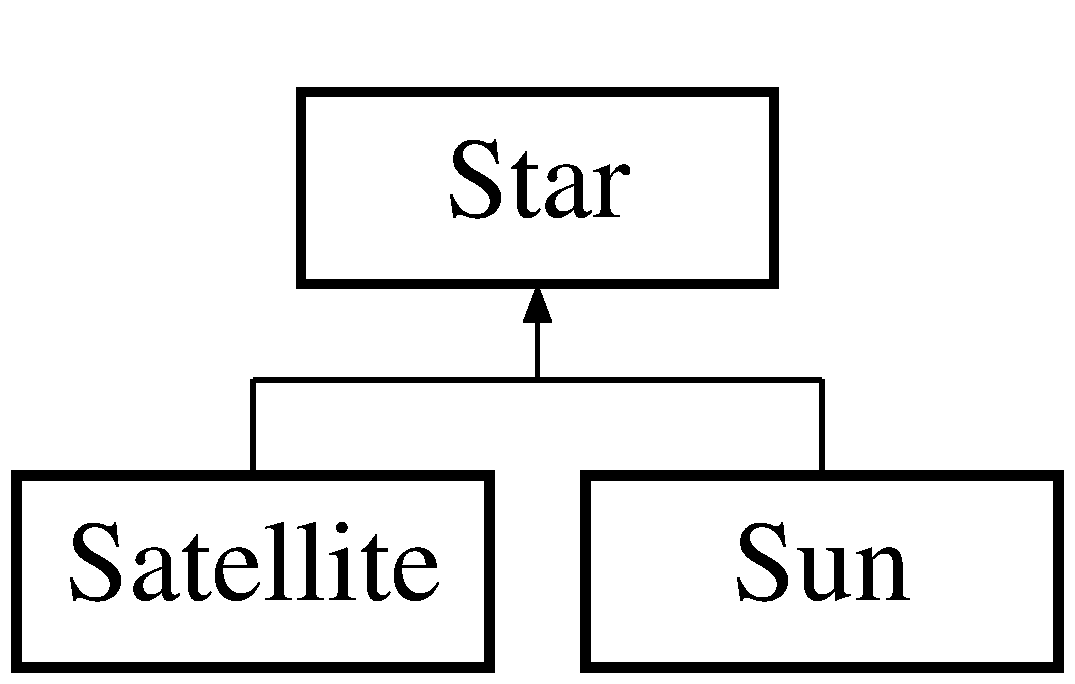
\includegraphics[height=2.000000cm]{class_star}
\end{center}
\end{figure}
\subsection*{Public Member Functions}
\begin{DoxyCompactItemize}
\item 
\hyperlink{class_star_a1d568f3308c55d5d5d138b606860b722}{Star} (double a\-Radius=0., double an\-Angle=0., double a\-Galaxy\-Limit=-\/1.)
\item 
\hypertarget{class_star_ab4572b2461408ef03d1d56f0b7c9b130}{void {\bfseries set\-Coordinates\-Polar} (double a\-Radius, double an\-Angle)}\label{class_star_ab4572b2461408ef03d1d56f0b7c9b130}

\item 
\hypertarget{class_star_a3dce898ff096b752b1ab57863e8d6622}{void {\bfseries set\-Radius} (double a\-Radius)}\label{class_star_a3dce898ff096b752b1ab57863e8d6622}

\item 
\hypertarget{class_star_a8e27c64ecb1cb2c9ff62372af8ca773a}{void {\bfseries set\-Angle} (double an\-Angle)}\label{class_star_a8e27c64ecb1cb2c9ff62372af8ca773a}

\item 
\hypertarget{class_star_a53f9a513fd6f5cacf8c3061b0c698349}{void {\bfseries set\-Coordinates\-Cartesian} (double an\-Abscissa, double an\-Ordinate)}\label{class_star_a53f9a513fd6f5cacf8c3061b0c698349}

\item 
\hypertarget{class_star_a591fe6d39b454840f336e6c8931f39ff}{void {\bfseries set\-Abscissa} (double an\-Abscissa)}\label{class_star_a591fe6d39b454840f336e6c8931f39ff}

\item 
\hypertarget{class_star_a7b2a9ca158383587cbde89d59eacfa4a}{void {\bfseries set\-Ordinate} (double an\-Ordinate)}\label{class_star_a7b2a9ca158383587cbde89d59eacfa4a}

\item 
\hypertarget{class_star_ad21eb659ca319c555df738d5b17a534a}{void {\bfseries set\-Color} (double red, double green, double blue, double alpha)}\label{class_star_ad21eb659ca319c555df738d5b17a534a}

\item 
\hypertarget{class_star_a5cbe56acf5caf0530baa7e58125f1a90}{void {\bfseries set\-Description} (std\-::string a\-Description)}\label{class_star_a5cbe56acf5caf0530baa7e58125f1a90}

\item 
\hypertarget{class_star_adf6a57bf8cee4c8bf40febbb71dff927}{void {\bfseries set\-Muted} (bool muted)}\label{class_star_adf6a57bf8cee4c8bf40febbb71dff927}

\item 
\hypertarget{class_star_a3b8c8edca0eb3ccc89a4b91227bc7d97}{void {\bfseries set\-Galaxy\-Limit} (double a\-Galaxy\-Limit)}\label{class_star_a3b8c8edca0eb3ccc89a4b91227bc7d97}

\item 
\hypertarget{class_star_a8791cc2c8764f7213379dccc47cb6327}{double {\bfseries get\-Radius} ()}\label{class_star_a8791cc2c8764f7213379dccc47cb6327}

\item 
\hypertarget{class_star_a8ccf772d6c9cbfae316d5826cbd9a005}{double {\bfseries get\-Angle} ()}\label{class_star_a8ccf772d6c9cbfae316d5826cbd9a005}

\item 
\hypertarget{class_star_a15a3dc0db429e55c800c5b223188d621}{double {\bfseries get\-Abscissa} ()}\label{class_star_a15a3dc0db429e55c800c5b223188d621}

\item 
\hypertarget{class_star_aeff266b94f5f11a0284936c7463504cc}{double {\bfseries get\-Ordinate} ()}\label{class_star_aeff266b94f5f11a0284936c7463504cc}

\item 
\hypertarget{class_star_ab3b191c54d8d42677845d2e5216bc3dd}{\hyperlink{structcolor}{color} {\bfseries get\-Color} ()}\label{class_star_ab3b191c54d8d42677845d2e5216bc3dd}

\item 
\hypertarget{class_star_aa87c110acd935d65ab862d0bd3ee662a}{std\-::string {\bfseries get\-Description} ()}\label{class_star_aa87c110acd935d65ab862d0bd3ee662a}

\item 
\hypertarget{class_star_a89b13cf4eabb12f59ba0e4286b351d9a}{bool {\bfseries get\-Muted} ()}\label{class_star_a89b13cf4eabb12f59ba0e4286b351d9a}

\item 
\hypertarget{class_star_acd0708d8166d6dba1edd61cab35f80bc}{double {\bfseries get\-Galaxy\-Limit} ()}\label{class_star_acd0708d8166d6dba1edd61cab35f80bc}

\item 
\hypertarget{class_star_a34d3229ef6683f7eb62ccbf22816f3c4}{double {\bfseries get\-Distance\-To\-Galaxy\-Limit} (double an\-Angle)}\label{class_star_a34d3229ef6683f7eb62ccbf22816f3c4}

\end{DoxyCompactItemize}
\subsection*{Protected Attributes}
\begin{DoxyCompactItemize}
\item 
\hypertarget{class_star_a687d043aec32f3851a6d07cb37bd5f60}{double {\bfseries m\-\_\-radius}}\label{class_star_a687d043aec32f3851a6d07cb37bd5f60}

\item 
\hypertarget{class_star_ac60a93823c3e79224202fd0e77654a83}{double {\bfseries m\-\_\-angle}}\label{class_star_ac60a93823c3e79224202fd0e77654a83}

\item 
\hypertarget{class_star_abd432e9947bf22fdd6dce0449017be00}{\hyperlink{structcolor}{color} {\bfseries m\-\_\-color}}\label{class_star_abd432e9947bf22fdd6dce0449017be00}

\item 
\hypertarget{class_star_a2b9dcdf04555f124c7730c2f2eedbbe2}{std\-::string {\bfseries m\-\_\-description}}\label{class_star_a2b9dcdf04555f124c7730c2f2eedbbe2}

\item 
\hypertarget{class_star_a8fdf5f31524c641c2a976be91104f3d2}{bool {\bfseries m\-\_\-muted}}\label{class_star_a8fdf5f31524c641c2a976be91104f3d2}

\item 
\hypertarget{class_star_a8bb66e389333e5ae54bb90264d87e043}{double {\bfseries m\-\_\-galaxy\-\_\-limit}}\label{class_star_a8bb66e389333e5ae54bb90264d87e043}

\end{DoxyCompactItemize}


\subsection{Detailed Description}
Hoa\-Library \-: A High Order Ambisonics Library Copyright (c) 2012-\/2013 Julien Colafrancesco, Pierre Guillot, Eliott Paris, C\-I\-C\-M, Universite Paris-\/8. All rights reserved.\-re Guillot, C\-I\-C\-M -\/ Université Paris 8 All rights reserved.

Website \-: \href{http://www.mshparisnord.fr/HoaLibrary/}{\tt http\-://www.\-mshparisnord.\-fr/\-Hoa\-Library/} Contacts \-: \href{mailto:cicm.mshparisnord@gmail.com}{\tt cicm.\-mshparisnord@gmail.\-com}

This file is part of H\-O\-A L\-I\-B\-R\-A\-R\-Y.

H\-O\-A L\-I\-B\-R\-A\-R\-Y is free software\-: you can redistribute it and/or modify it under the terms of the G\-N\-U General Public License as published by the Free Software Foundation, either version 3 of the License, or (at your option) any later version.

This program is distributed in the hope that it will be useful, but W\-I\-T\-H\-O\-U\-T A\-N\-Y W\-A\-R\-R\-A\-N\-T\-Y; without even the implied warranty of M\-E\-R\-C\-H\-A\-N\-T\-A\-B\-I\-L\-I\-T\-Y or F\-I\-T\-N\-E\-S\-S F\-O\-R A P\-A\-R\-T\-I\-C\-U\-L\-A\-R P\-U\-R\-P\-O\-S\-E. See the G\-N\-U General Public License for more details.

You should have received a copy of the G\-N\-U General Public License along with this program. If not, see \href{http://www.gnu.org/licenses/}{\tt http\-://www.\-gnu.\-org/licenses/}. 

\subsection{Constructor \& Destructor Documentation}
\hypertarget{class_star_a1d568f3308c55d5d5d138b606860b722}{\index{Star@{Star}!Star@{Star}}
\index{Star@{Star}!Star@{Star}}
\subsubsection[{Star}]{\setlength{\rightskip}{0pt plus 5cm}Star\-::\-Star (
\begin{DoxyParamCaption}
\item[{double}]{a\-Radius = {\ttfamily 0.}, }
\item[{double}]{an\-Angle = {\ttfamily 0.}, }
\item[{double}]{a\-Galaxy\-Limit = {\ttfamily -\/1.}}
\end{DoxyParamCaption}
)}}\label{class_star_a1d568f3308c55d5d5d138b606860b722}
Hoa\-Library \-: A High Order Ambisonics Library Copyright (c) 2012-\/2013 Julien Colafrancesco, Pierre Guillot, Eliott Paris, C\-I\-C\-M, Universite Paris-\/8. All rights reserved.\-re Guillot, C\-I\-C\-M -\/ Université Paris 8 All rights reserved.

Website \-: \href{http://www.mshparisnord.fr/HoaLibrary/}{\tt http\-://www.\-mshparisnord.\-fr/\-Hoa\-Library/} Contacts \-: \href{mailto:cicm.mshparisnord@gmail.com}{\tt cicm.\-mshparisnord@gmail.\-com}

This file is part of H\-O\-A L\-I\-B\-R\-A\-R\-Y.

H\-O\-A L\-I\-B\-R\-A\-R\-Y is free software\-: you can redistribute it and/or modify it under the terms of the G\-N\-U General Public License as published by the Free Software Foundation, either version 3 of the License, or (at your option) any later version.

This program is distributed in the hope that it will be useful, but W\-I\-T\-H\-O\-U\-T A\-N\-Y W\-A\-R\-R\-A\-N\-T\-Y; without even the implied warranty of M\-E\-R\-C\-H\-A\-N\-T\-A\-B\-I\-L\-I\-T\-Y or F\-I\-T\-N\-E\-S\-S F\-O\-R A P\-A\-R\-T\-I\-C\-U\-L\-A\-R P\-U\-R\-P\-O\-S\-E. See the G\-N\-U General Public License for more details.

You should have received a copy of the G\-N\-U General Public License along with this program. If not, see \href{http://www.gnu.org/licenses/}{\tt http\-://www.\-gnu.\-org/licenses/}. 

The documentation for this class was generated from the following files\-:\begin{DoxyCompactItemize}
\item 
/\-Users/\-Pierre/\-Source\-Tree/\-Hoa\-Library/\-Sources/hoa\-Galaxy/Ambisonics\-Star.\-h\item 
/\-Users/\-Pierre/\-Source\-Tree/\-Hoa\-Library/\-Sources/hoa\-Galaxy/Ambisonics\-Star.\-cpp\end{DoxyCompactItemize}

\hypertarget{class_sun}{\section{Sun Class Reference}
\label{class_sun}\index{Sun@{Sun}}
}


{\ttfamily \#include $<$Ambisonics\-Sun.\-h$>$}

Inheritance diagram for Sun\-:\begin{figure}[H]
\begin{center}
\leavevmode
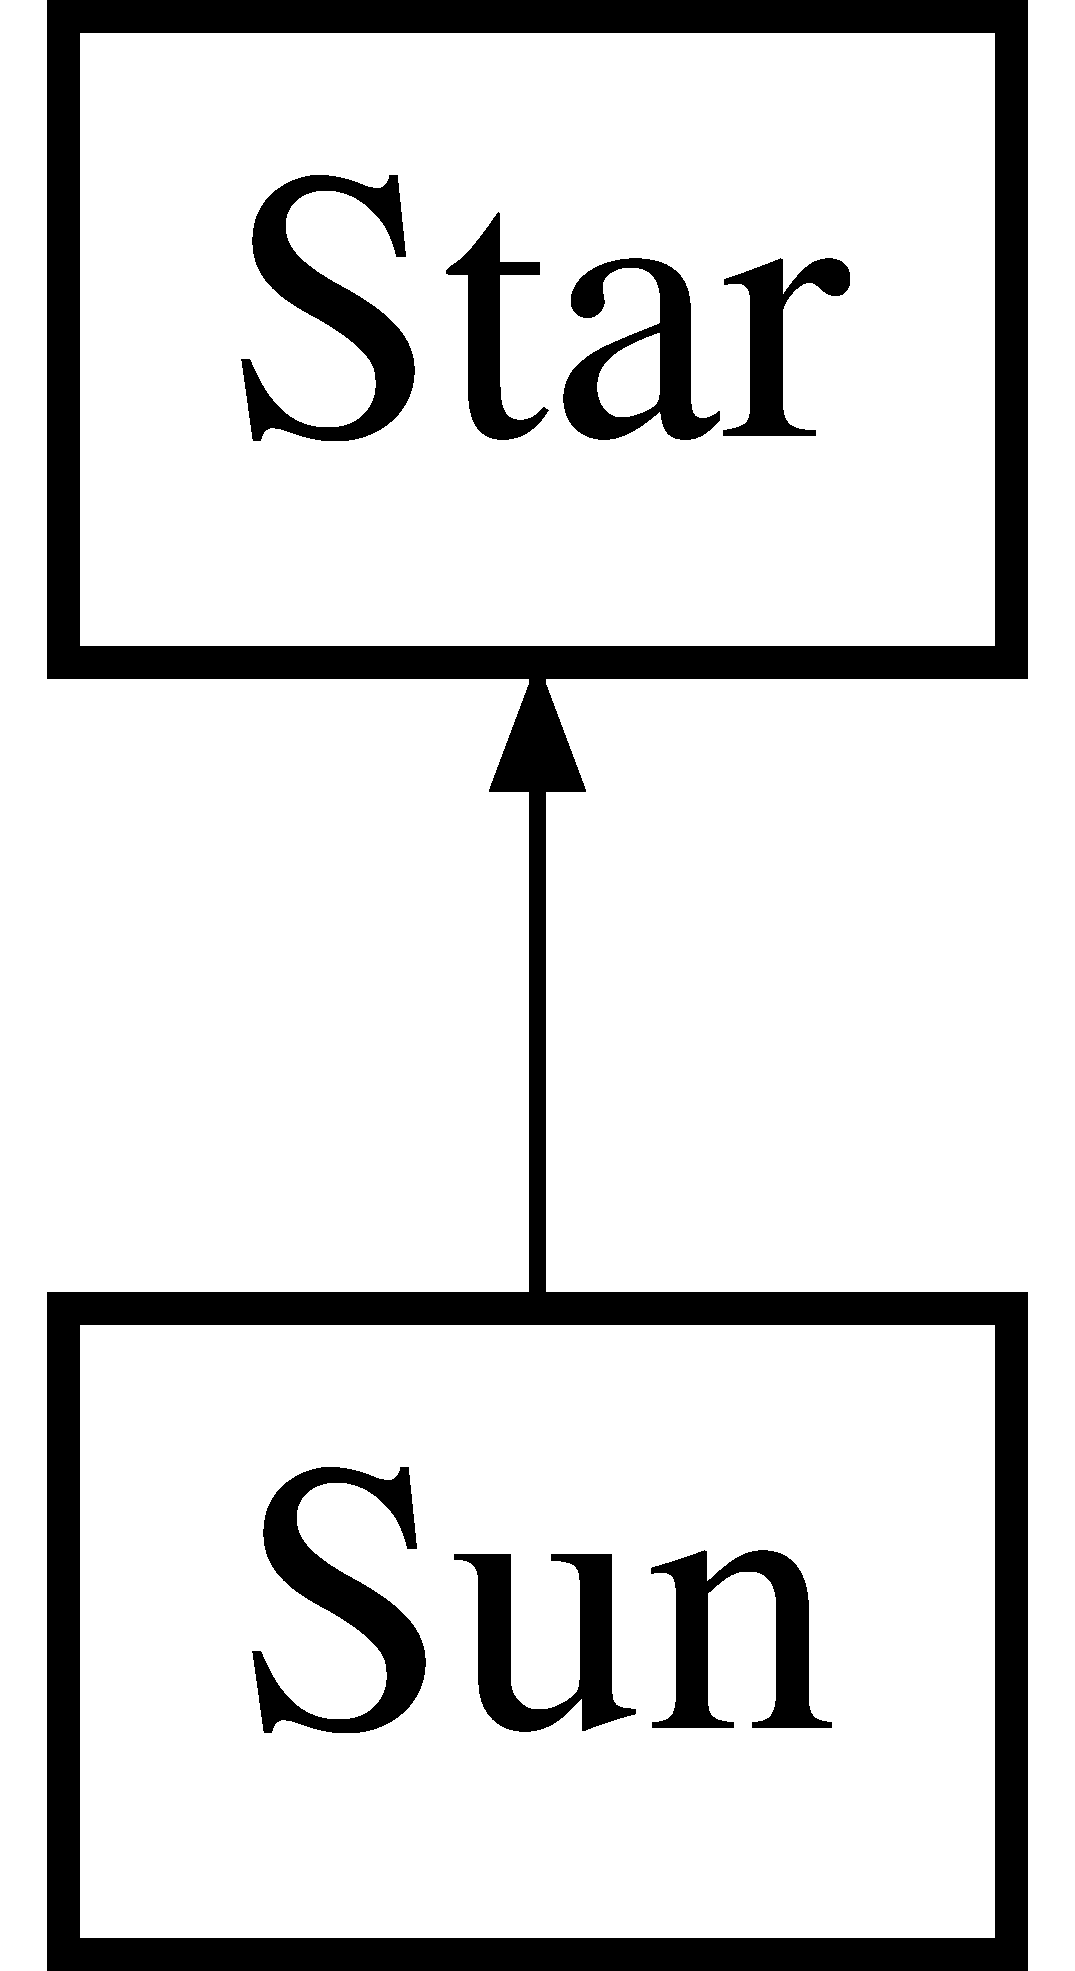
\includegraphics[height=2.000000cm]{class_sun}
\end{center}
\end{figure}
\subsection*{Public Member Functions}
\begin{DoxyCompactItemize}
\item 
\hyperlink{class_sun_a6faf7873a49c90937f63af0bd0208eab}{Sun} (double a\-Radius=0., double an\-Angle=0., double a\-Maximum\-Radius=-\/1.)
\end{DoxyCompactItemize}
\subsection*{Additional Inherited Members}


\subsection{Detailed Description}
Hoa\-Library \-: A High Order Ambisonics Library Copyright (c) 2012-\/2013 Julien Colafrancesco, Pierre Guillot, Eliott Paris, C\-I\-C\-M, Universite Paris-\/8. All rights reserved.\-re Guillot, C\-I\-C\-M -\/ Université Paris 8 All rights reserved.

Website \-: \href{http://www.mshparisnord.fr/HoaLibrary/}{\tt http\-://www.\-mshparisnord.\-fr/\-Hoa\-Library/} Contacts \-: \href{mailto:cicm.mshparisnord@gmail.com}{\tt cicm.\-mshparisnord@gmail.\-com}

This file is part of H\-O\-A L\-I\-B\-R\-A\-R\-Y.

H\-O\-A L\-I\-B\-R\-A\-R\-Y is free software\-: you can redistribute it and/or modify it under the terms of the G\-N\-U General Public License as published by the Free Software Foundation, either version 3 of the License, or (at your option) any later version.

This program is distributed in the hope that it will be useful, but W\-I\-T\-H\-O\-U\-T A\-N\-Y W\-A\-R\-R\-A\-N\-T\-Y; without even the implied warranty of M\-E\-R\-C\-H\-A\-N\-T\-A\-B\-I\-L\-I\-T\-Y or F\-I\-T\-N\-E\-S\-S F\-O\-R A P\-A\-R\-T\-I\-C\-U\-L\-A\-R P\-U\-R\-P\-O\-S\-E. See the G\-N\-U General Public License for more details.

You should have received a copy of the G\-N\-U General Public License along with this program. If not, see \href{http://www.gnu.org/licenses/}{\tt http\-://www.\-gnu.\-org/licenses/}. 

\subsection{Constructor \& Destructor Documentation}
\hypertarget{class_sun_a6faf7873a49c90937f63af0bd0208eab}{\index{Sun@{Sun}!Sun@{Sun}}
\index{Sun@{Sun}!Sun@{Sun}}
\subsubsection[{Sun}]{\setlength{\rightskip}{0pt plus 5cm}Sun\-::\-Sun (
\begin{DoxyParamCaption}
\item[{double}]{a\-Radius = {\ttfamily 0.}, }
\item[{double}]{an\-Angle = {\ttfamily 0.}, }
\item[{double}]{a\-Maximum\-Radius = {\ttfamily -\/1.}}
\end{DoxyParamCaption}
)}}\label{class_sun_a6faf7873a49c90937f63af0bd0208eab}
Hoa\-Library \-: A High Order Ambisonics Library Copyright (c) 2012-\/2013 Julien Colafrancesco, Pierre Guillot, Eliott Paris, C\-I\-C\-M, Universite Paris-\/8. All rights reserved.\-re Guillot, C\-I\-C\-M -\/ Université Paris 8 All rights reserved.

Website \-: \href{http://www.mshparisnord.fr/HoaLibrary/}{\tt http\-://www.\-mshparisnord.\-fr/\-Hoa\-Library/} Contacts \-: \href{mailto:cicm.mshparisnord@gmail.com}{\tt cicm.\-mshparisnord@gmail.\-com}

This file is part of H\-O\-A L\-I\-B\-R\-A\-R\-Y.

H\-O\-A L\-I\-B\-R\-A\-R\-Y is free software\-: you can redistribute it and/or modify it under the terms of the G\-N\-U General Public License as published by the Free Software Foundation, either version 3 of the License, or (at your option) any later version.

This program is distributed in the hope that it will be useful, but W\-I\-T\-H\-O\-U\-T A\-N\-Y W\-A\-R\-R\-A\-N\-T\-Y; without even the implied warranty of M\-E\-R\-C\-H\-A\-N\-T\-A\-B\-I\-L\-I\-T\-Y or F\-I\-T\-N\-E\-S\-S F\-O\-R A P\-A\-R\-T\-I\-C\-U\-L\-A\-R P\-U\-R\-P\-O\-S\-E. See the G\-N\-U General Public License for more details.

You should have received a copy of the G\-N\-U General Public License along with this program. If not, see \href{http://www.gnu.org/licenses/}{\tt http\-://www.\-gnu.\-org/licenses/}. 

The documentation for this class was generated from the following files\-:\begin{DoxyCompactItemize}
\item 
/\-Users/\-Pierre/\-Source\-Tree/\-Hoa\-Library/\-Sources/hoa\-Galaxy/Ambisonics\-Sun.\-h\item 
/\-Users/\-Pierre/\-Source\-Tree/\-Hoa\-Library/\-Sources/hoa\-Galaxy/Ambisonics\-Sun.\-cpp\end{DoxyCompactItemize}

\hypertarget{class_tools}{\section{Tools Class Reference}
\label{class_tools}\index{Tools@{Tools}}
}


\subsection{Detailed Description}


Definition at line 68 of file Cicm\-Tools.\-h.



The documentation for this class was generated from the following file\-:\begin{DoxyCompactItemize}
\item 
/\-Users/\-Pierre/\-Source\-Tree/\-Hoa\-Library/\-Sources/\-Cicm\-Library/Cicm\-Tools.\-h\end{DoxyCompactItemize}

\hypertarget{struct_velocity}{\section{Velocity Struct Reference}
\label{struct_velocity}\index{Velocity@{Velocity}}
}


\subsection{Detailed Description}


Definition at line 59 of file Boids\-Manager.\-h.



The documentation for this struct was generated from the following file\-:\begin{DoxyCompactItemize}
\item 
/\-Users/elioton/\-Documents/programmation/\-C\-I\-C\-M/source\-Tree/\-Hoa\-Library/\-Sources/hoa\-Boids/Boids\-Manager.\-h\end{DoxyCompactItemize}

%--- End generated contents ---

% Index
\newpage
\phantomsection
\addcontentsline{toc}{part}{Index}
\printindex

\end{document}
